\documentclass[]{book}
\usepackage{lmodern}
\usepackage{amssymb,amsmath}
\usepackage{ifxetex,ifluatex}
\usepackage{fixltx2e} % provides \textsubscript
\ifnum 0\ifxetex 1\fi\ifluatex 1\fi=0 % if pdftex
  \usepackage[T1]{fontenc}
  \usepackage[utf8]{inputenc}
\else % if luatex or xelatex
  \ifxetex
    \usepackage{mathspec}
  \else
    \usepackage{fontspec}
  \fi
  \defaultfontfeatures{Ligatures=TeX,Scale=MatchLowercase}
\fi
% use upquote if available, for straight quotes in verbatim environments
\IfFileExists{upquote.sty}{\usepackage{upquote}}{}
% use microtype if available
\IfFileExists{microtype.sty}{%
\usepackage[]{microtype}
\UseMicrotypeSet[protrusion]{basicmath} % disable protrusion for tt fonts
}{}
\PassOptionsToPackage{hyphens}{url} % url is loaded by hyperref
\usepackage[unicode=true]{hyperref}
\hypersetup{
            pdftitle={Prácticas de Tecnologías de Gestión y Manipulación de Datos},
            pdfauthor={Guillermo López Taboada (guillermo.lopez.taboada@udc.es) y Rubén F. Casal (ruben.fcasal@udc.es)},
            pdfborder={0 0 0},
            breaklinks=true}
\urlstyle{same}  % don't use monospace font for urls
\usepackage{natbib}
\bibliographystyle{apalike}
\usepackage{color}
\usepackage{fancyvrb}
\newcommand{\VerbBar}{|}
\newcommand{\VERB}{\Verb[commandchars=\\\{\}]}
\DefineVerbatimEnvironment{Highlighting}{Verbatim}{commandchars=\\\{\}}
% Add ',fontsize=\small' for more characters per line
\usepackage{framed}
\definecolor{shadecolor}{RGB}{248,248,248}
\newenvironment{Shaded}{\begin{snugshade}}{\end{snugshade}}
\newcommand{\KeywordTok}[1]{\textcolor[rgb]{0.13,0.29,0.53}{\textbf{#1}}}
\newcommand{\DataTypeTok}[1]{\textcolor[rgb]{0.13,0.29,0.53}{#1}}
\newcommand{\DecValTok}[1]{\textcolor[rgb]{0.00,0.00,0.81}{#1}}
\newcommand{\BaseNTok}[1]{\textcolor[rgb]{0.00,0.00,0.81}{#1}}
\newcommand{\FloatTok}[1]{\textcolor[rgb]{0.00,0.00,0.81}{#1}}
\newcommand{\ConstantTok}[1]{\textcolor[rgb]{0.00,0.00,0.00}{#1}}
\newcommand{\CharTok}[1]{\textcolor[rgb]{0.31,0.60,0.02}{#1}}
\newcommand{\SpecialCharTok}[1]{\textcolor[rgb]{0.00,0.00,0.00}{#1}}
\newcommand{\StringTok}[1]{\textcolor[rgb]{0.31,0.60,0.02}{#1}}
\newcommand{\VerbatimStringTok}[1]{\textcolor[rgb]{0.31,0.60,0.02}{#1}}
\newcommand{\SpecialStringTok}[1]{\textcolor[rgb]{0.31,0.60,0.02}{#1}}
\newcommand{\ImportTok}[1]{#1}
\newcommand{\CommentTok}[1]{\textcolor[rgb]{0.56,0.35,0.01}{\textit{#1}}}
\newcommand{\DocumentationTok}[1]{\textcolor[rgb]{0.56,0.35,0.01}{\textbf{\textit{#1}}}}
\newcommand{\AnnotationTok}[1]{\textcolor[rgb]{0.56,0.35,0.01}{\textbf{\textit{#1}}}}
\newcommand{\CommentVarTok}[1]{\textcolor[rgb]{0.56,0.35,0.01}{\textbf{\textit{#1}}}}
\newcommand{\OtherTok}[1]{\textcolor[rgb]{0.56,0.35,0.01}{#1}}
\newcommand{\FunctionTok}[1]{\textcolor[rgb]{0.00,0.00,0.00}{#1}}
\newcommand{\VariableTok}[1]{\textcolor[rgb]{0.00,0.00,0.00}{#1}}
\newcommand{\ControlFlowTok}[1]{\textcolor[rgb]{0.13,0.29,0.53}{\textbf{#1}}}
\newcommand{\OperatorTok}[1]{\textcolor[rgb]{0.81,0.36,0.00}{\textbf{#1}}}
\newcommand{\BuiltInTok}[1]{#1}
\newcommand{\ExtensionTok}[1]{#1}
\newcommand{\PreprocessorTok}[1]{\textcolor[rgb]{0.56,0.35,0.01}{\textit{#1}}}
\newcommand{\AttributeTok}[1]{\textcolor[rgb]{0.77,0.63,0.00}{#1}}
\newcommand{\RegionMarkerTok}[1]{#1}
\newcommand{\InformationTok}[1]{\textcolor[rgb]{0.56,0.35,0.01}{\textbf{\textit{#1}}}}
\newcommand{\WarningTok}[1]{\textcolor[rgb]{0.56,0.35,0.01}{\textbf{\textit{#1}}}}
\newcommand{\AlertTok}[1]{\textcolor[rgb]{0.94,0.16,0.16}{#1}}
\newcommand{\ErrorTok}[1]{\textcolor[rgb]{0.64,0.00,0.00}{\textbf{#1}}}
\newcommand{\NormalTok}[1]{#1}
\usepackage{longtable,booktabs}
% Fix footnotes in tables (requires footnote package)
\IfFileExists{footnote.sty}{\usepackage{footnote}\makesavenoteenv{long table}}{}
\usepackage{graphicx,grffile}
\makeatletter
\def\maxwidth{\ifdim\Gin@nat@width>\linewidth\linewidth\else\Gin@nat@width\fi}
\def\maxheight{\ifdim\Gin@nat@height>\textheight\textheight\else\Gin@nat@height\fi}
\makeatother
% Scale images if necessary, so that they will not overflow the page
% margins by default, and it is still possible to overwrite the defaults
% using explicit options in \includegraphics[width, height, ...]{}
\setkeys{Gin}{width=\maxwidth,height=\maxheight,keepaspectratio}
\IfFileExists{parskip.sty}{%
\usepackage{parskip}
}{% else
\setlength{\parindent}{0pt}
\setlength{\parskip}{6pt plus 2pt minus 1pt}
}
\setlength{\emergencystretch}{3em}  % prevent overfull lines
\providecommand{\tightlist}{%
  \setlength{\itemsep}{0pt}\setlength{\parskip}{0pt}}
\setcounter{secnumdepth}{5}
% Redefines (sub)paragraphs to behave more like sections
\ifx\paragraph\undefined\else
\let\oldparagraph\paragraph
\renewcommand{\paragraph}[1]{\oldparagraph{#1}\mbox{}}
\fi
\ifx\subparagraph\undefined\else
\let\oldsubparagraph\subparagraph
\renewcommand{\subparagraph}[1]{\oldsubparagraph{#1}\mbox{}}
\fi

% set default figure placement to htbp
\makeatletter
\def\fps@figure{htbp}
\makeatother

\usepackage{booktabs}
\usepackage{amsthm}
%\usepackage{animate}
\ifxetex
  \usepackage{polyglossia}
  \setmainlanguage{spanish}
  % Tabla en lugar de cuadro
  \gappto\captionsspanish{\renewcommand{\tablename}{Tabla}
          \renewcommand{\listtablename}{Índice de tablas}}

\else
  \usepackage[spanish,es-tabla]{babel}
\fi
\makeatletter
\def\thm@space@setup{%
  \thm@preskip=8pt plus 2pt minus 4pt
  \thm@postskip=\thm@preskip
}
\makeatother

\title{Prácticas de Tecnologías de Gestión y Manipulación de Datos}
\author{Guillermo López Taboada
(\href{mailto:guillermo.lopez.taboada@udc.es}{\nolinkurl{guillermo.lopez.taboada@udc.es}})
y Rubén F. Casal
(\href{mailto:ruben.fcasal@udc.es}{\nolinkurl{ruben.fcasal@udc.es}})}
\date{2020-09-21}

\begin{document}
\maketitle

{
\setcounter{tocdepth}{1}
\tableofcontents
}
\chapter*{Prólogo}\label{pruxf3logo}
\addcontentsline{toc}{chapter}{Prólogo}

Este libro contiene algunas de las prácticas de la asignatura de
\href{http://eamo.usc.es/pub/mte/index.php/es/?option=com_content\&view=article\&id=2202\&idm=38\&a\%C3\%B1o=2020}{Tecnologías
de Gestión de Datos} del \href{http://eio.usc.es/pub/mte}{Máster
interuniversitario en Técnicas Estadísticas}).

Este libro ha sido escrito en
\href{http://rmarkdown.rstudio.com}{R-Markdown} empleando el paquete
\href{https://bookdown.org/yihui/bookdown/}{\texttt{bookdown}} y está
disponible en el repositorio Github:
\href{https://github.com/gltaboada/tgdbook}{gltaboada/tgdbook}. Se puede
acceder a la versión en línea a través del siguiente enlace:

\url{https://gltaboada.github.io/tgdbook}.

donde puede descargarse en formato
\href{https://gltaboada.github.io/tgdbook/Practicas_de_TGD.pdf}{pdf}.

Para ejecutar los ejemplos mostrados en el libro será necesario tener
instalados los siguientes paquetes:
\href{https://dplyr.tidyverse.org}{\texttt{dplyr}} (colección
\href{https://www.tidyverse.org/}{\texttt{tidyverse}}),
\href{https://tidyr.tidyverse.org}{\texttt{tidyr}},
\href{https://stringr.tidyverse.org}{\texttt{stringr}},
\href{https://readxl.tidyverse.org}{\texttt{readxl}} ,
\href{https://cran.r-project.org/web/packages/openxlsx/index.html}{\texttt{openxlsx}},
\href{https://cran.r-project.org/web/packages/RODBC/index.html}{\texttt{RODBC}},
\href{https://cran.r-project.org/web/packages/sqldf/index.html}{\texttt{sqldf}},
\href{https://r-dbi.github.io/RSQLite}{\texttt{RSQLite}},
\href{https://cran.r-project.org/web/packages/foreign/index.html}{\texttt{foreign}},
\href{https://cran.r-project.org/web/packages/SparkR/index.html}{\texttt{SparkR}},
\href{https://cran.r-project.org/web/packages/magrittr/index.html}{\texttt{magrittr}},
\href{https://yihui.name/knitr}{\texttt{knitr}} Por ejemplo mediante los
comandos:

\begin{Shaded}
\begin{Highlighting}[]
\NormalTok{pkgs <-}\StringTok{ }\KeywordTok{c}\NormalTok{(}\StringTok{'dplyr'}\NormalTok{, }\StringTok{'tidyr'}\NormalTok{, }\StringTok{'stringr'}\NormalTok{, }\StringTok{'readxl'}\NormalTok{, }\StringTok{'openxlsx'}\NormalTok{, }\StringTok{'magrittr'}\NormalTok{, }
          \StringTok{'RODBC'}\NormalTok{, }\StringTok{'sqldf'}\NormalTok{, }\StringTok{'RSQLite'}\NormalTok{, }\StringTok{'foreign'}\NormalTok{, }\StringTok{'SparkR'}\NormalTok{, }\StringTok{'knitr'}\NormalTok{)}
\CommentTok{# install.packages(pkgs, dependencies=TRUE)}
\KeywordTok{install.packages}\NormalTok{(}\KeywordTok{setdiff}\NormalTok{(pkgs, }\KeywordTok{installed.packages}\NormalTok{()[,}\StringTok{'Package'}\NormalTok{]), }\DataTypeTok{dependencies =} \OtherTok{TRUE}\NormalTok{)}
\end{Highlighting}
\end{Shaded}

Para generar el libro (compilar) se recomendaría consultar el libro de
\href{https://rubenfcasal.github.io/bookdown_intro}{``Escritura de
libros con bookdown''} en castellano.

\includegraphics[width=1.22in]{images/by-nc-nd-88x31}

Este obra está bajo una licencia de
\href{https://creativecommons.org/licenses/by-nc-nd/4.0/deed.es_ES}{Creative
Commons Reconocimiento-NoComercial-SinObraDerivada 4.0 Internacional}
(esperamos poder liberarlo bajo una licencia menos restrictiva más
adelante\ldots{}).

\chapter{Introducción a las Tecnologías de Gestión y Manipulación de
Datos}\label{introducciuxf3n-a-las-tecnologuxedas-de-gestiuxf3n-y-manipulaciuxf3n-de-datos}

La información relevante de la materia está disponible en la guía
docente y la ficha de la asignatura

En particular, los resultados de aprendizaje son:

\begin{itemize}
\item
  Manejar de forma autónoma y solvente el software necesario para
  acceder a conjuntos de datos en entornos profesionales y/o en la nube.
\item
  Saber gestionar conjuntos de datos masivos en un entorno
  multidisciplinar que permita la participación en proyectos
  profesionales complejos que requieran el uso de técnicas estadísticas.
\item
  Saber relacionar el software de diseño y gestión de bases de datos con
  el específicamente implementado para el análisis de datos.
\end{itemize}

\section{Contenidos}\label{contenidos}

\begin{enumerate}
\def\labelenumi{\arabic{enumi}.}
\tightlist
\item
  Introducción al lenguaje SQL

  \begin{itemize}
  \tightlist
  \item
    Bases de datos relacionales
  \item
    Sintaxis SQL
  \item
    Conexión con bases de datos desde R
  \end{itemize}
\item
  Introducción a tecnologías NoSQL

  \begin{itemize}
  \tightlist
  \item
    Conceptos y tipos de bases de datos NoSQL (documental, columnar,
    clave/valor y de grafos)
  \item
    Conexión de R a NoSQL
  \end{itemize}
\item
  Tecnologías para el tratamiento de datos masivos

  \begin{itemize}
  \tightlist
  \item
    Tecnologías Big Data
  \item
    Visualización y generación de cuadros de mando
  \item
    Introducción al análisis de datos masivos.
  \end{itemize}
\end{enumerate}

\section{Planificación (tentativa)}\label{planificaciuxf3n-tentativa}

La impartición de los contenidos durante el curso dependerá de los
conocimientos de partida y la asimilación de los conceptos. Para
completar nuestra visión de los conocimientos previos os requerimos
completar este formulario en la primera sesión de clase:
\url{https://forms.gle/9HR5iFHXoLowrCHLA}

\begin{itemize}
\item
  Clase 1 (14/9): Presentación e introducción a Tema 1.
\item
  Clase 2 (17/9): Tema 1: Introducción a SQL
\item
  Clase 3 (21/9-RFC): Seminario Manipulación de datos con R
\item
  Clase 4 (24/9-RFC): Seminario Manipulación de datos con dplyr
\item
  Clase 5 (28/9): Tema 1: Ejercicios SQL
\item
  Clase 6 (1/10): Tema 1: Ejercicios SQL
\item
  Clase 7 (5/10): Tema 2: Introducción a NoSQL
\item
  Clase 8 (8/10): Tema 2: Ejercicios NoSQL
\item
  Clase 9 (19/10): Tema 2: Ejercicios con formatos Open Data
\item
  Clase 10 (26/10): Tema 3: Ecosistema Big Data
\item
  Clase 11-20 (2/11 al 3/12): Tema 3: Ecosistema Big Data (teoría,
  práctica) + Seminario de aprendizaje estadístico (3 sesiones con RFC)
\end{itemize}

No tendremos clase el 7 de Diciembre.

\begin{itemize}
\tightlist
\item
  Clases 21-23 (10, 14 y 17/12): Tema 3: Ejercicios Big Data
\end{itemize}

\subsection{Evaluación}\label{evaluaciuxf3n}

\begin{itemize}
\item
  \textbf{Examen} (60\%): El examen de la materia evaluará los
  siguientes aspectos: Conceptos de la materia: Dominio de los
  conocimientos teóricos y operativos de la materia. Asimilación
  práctica de materia: Asimilación y comprensión de los conocimientos
  teóricos y operativos de la materia.
\item
  \textbf{Prácticas de laboratorio} (30\%): Evaluación de las prácticas
  de laboratorio desarrolladas por los estudiantes.
\item
  \textbf{Trabajos tutelados} (10\%): Evaluación de los trabajos
  tutelados desarrollados por los estudiantes.
\end{itemize}

\subsubsection{Observaciones sobre la
evaluación:}\label{observaciones-sobre-la-evaluaciuxf3n}

\begin{itemize}
\item
  Las prácticas de laboratorio se realizarán de forma individual, así
  como el trabajo tutelado que es opcional. En caso de no realizar el
  trabajo tutelado los estudiantes tendrán un 67\% de nota del examen y
  un 33\% de prácticas de laboratorio. El plazo para realizar las 3
  prácticas será indicado en la presentación de la práctica. El plazo
  para la entrega de los trabajos tutelados es el último día de clase de
  la asignatura.
\item
  El estudiante que quiera realizar un trabajo tutelado ha de hablar (o
  mediante correo electrónico) con los profesores para validar y
  confirmar el tema y alcance del trabajo tutelado.
\item
  Para poder aprobar la asignatura en la primera oportunidad será
  necesario obtener como mínimo el 30\% de la nota máxima de la suma de
  las prácticas de laboratorio y trabajos tutelados e, igualmente, el
  30\% de la nota máxima final de la Prueba mixta (examen), y tener una
  nota total (prácticas más trabajos tutelados más prueba mixta) igual o
  superior al 50\% de la nota máxima.
\item
  En la segunda oportunidad solamente se podrá recuperar la nota del
  examen. Las notas de prácticas y de trabajos tutelados serán las
  obtenidas durante el curso. Para los alumnos que utilicen la
  oportunidad adelantada de diciembre se utilizarán las notas de
  prácticas y trabajos tutelados que obtuvieran en su último curso. En
  esta oportunidad solo será necesario para aprobar obtener una nota
  total igual o superior al 50\% de la nota máxima.
\item
  Una vez que un estudiante es evaluado en una práctica de laboratorio o
  en un trabajo tutelado implica que será calificado. Por tanto, la
  calificación ``No Presentado'' no es posible una vez que una
  práctica/trabajo ha sido evaluada.
\end{itemize}

\section{Fuentes de información:}\label{fuentes-de-informaciuxf3n}

\subsection{Básica}\label{buxe1sica}

\begin{itemize}
\item
  Daroczi, G. (2015). Mastering Data Analysis with R. Packt Publishing
\item
  Grolemund, G. y Wickham, H. (2016). R for Data Science.
  \url{https://r4ds.had.co.nz/} \& O'Reilly
\item
  Silberschatz, A., Korth, H. y Sudarshan, S. (2014). Fundamentos de
  Bases de Datos. Mc Graw Hill
\item
  Rubén Fernández Casal (\href{https://rubenfcasal.github.io}{R
  Machinery}):

  \begin{itemize}
  \item
    \href{https://rubenfcasal.github.io/intror}{Introducción al Análisis
    de Datos con R} (con Javier Roca y Julián Costa)
  \item
    \href{https://rubenfcasal.github.io/post/ayuda-y-recursos-para-el-aprendizaje-de-r}{Ayuda
    y Recursos para el Aprendizaje de R}
  \item
    \href{https://rubenfcasal.github.io/bookdown_intro}{Escritura de
    libros con el paquete bookdown} (con Tomás Cotos)
  \item
    \href{https://rubenfcasal.github.io/bookdown_intro/rmarkdown.html}{Apéndice
    introducción a Rmarkdown}
  \item
    \href{https://rubenfcasal.github.io/post/presentaciones/AnalisisDatosR.pdf}{Pesentación
    análisis de datos con R}
  \end{itemize}
\end{itemize}

\subsection{Complementaria:}\label{complementaria}

\begin{itemize}
\tightlist
\item
  Wes McKinney (2017). Python for Data Analysis: Data Wrangling with
  Pandas, NumPy, and IPython. O'Reilly (2ª ed.)
\item
  Tom White (2015). Hadoop: The Definitive Guide. O'Reilly (4ª ed.)
\item
  Alex Holmes (2014). Hadoop in practice. Manning (2ª ed.)
\item
  Centro de Supercomputación de Galicia (2019). Servicio de Big Data del
  CESGA. \url{https://bigdata.cesga.es/}
\end{itemize}

\chapter{Manipulación de datos con
R}\label{manipulaciuxf3n-de-datos-con-r}

En el proceso de análisis de datos, al margen de su obtención y
organización, una de las primeras etapas es el acceso y la manipulación
de los datos (ver Figura \ref{fig:esquema2}). En este capítulo se
repasarán brevemente las principales herramientas disponibles en el
paquete base de R para ello. Posteriormente en el Capítulo \ref{dplyr}
se mostrará como alternativa el uso del paquete
\href{https://dplyr.tidyverse.org/index.html}{\texttt{dplyr}}.

\begin{figure}[!htb]

{\centering 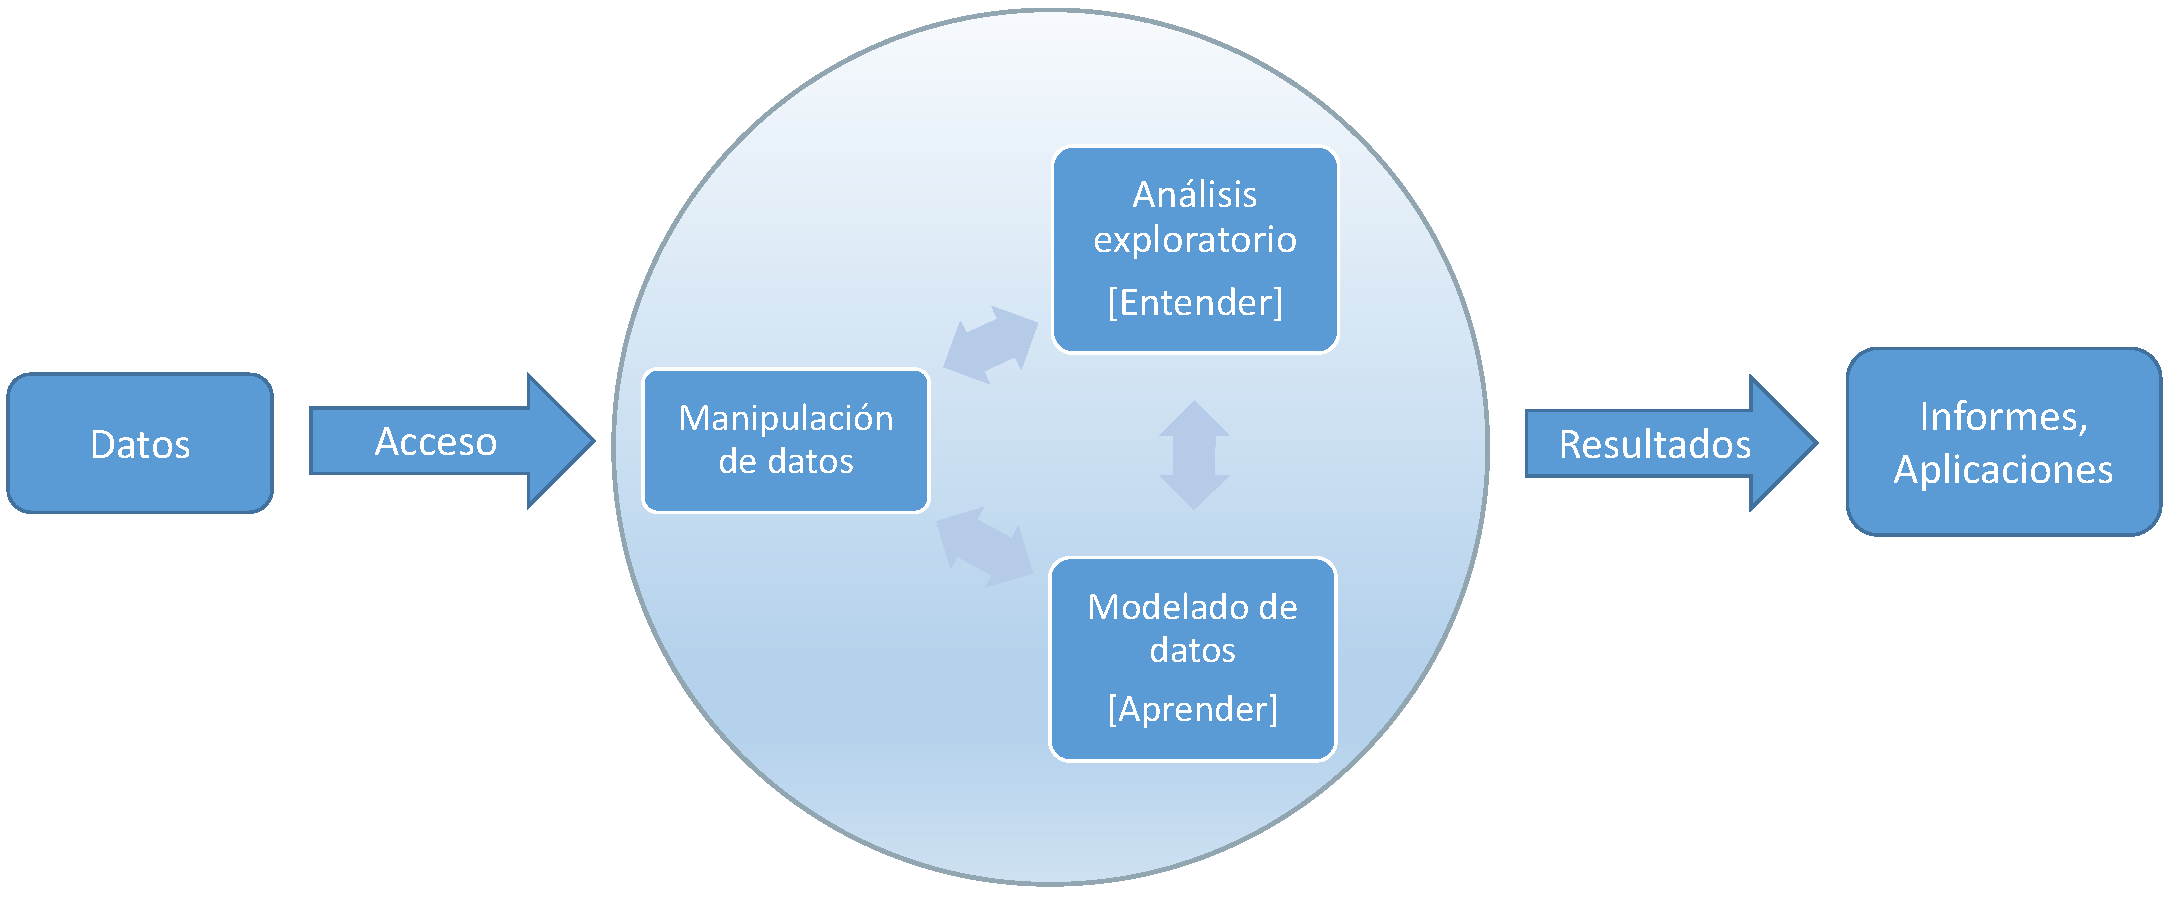
\includegraphics[width=0.8\linewidth]{images/esquema2} 

}

\caption{Etapas del proceso}\label{fig:esquema2}
\end{figure}

\section{Lectura, importación y exportación de
datos}\label{lectura-importaciuxf3n-y-exportaciuxf3n-de-datos}

Además de la introducción directa, R es capaz de importar datos externos
en múltiples formatos:

\begin{itemize}
\item
  bases de datos disponibles en librerías de R
\item
  archivos de texto en formato ASCII
\item
  archivos en otros formatos: Excel, SPSS, \ldots{}
\item
  bases de datos relacionales: MySQL, Oracle, \ldots{}
\item
  formatos web: HTML, XML, JSON, \ldots{}
\item
  \ldots{}.
\end{itemize}

\subsection{Formato de datos de R}\label{formato-de-datos-de-r}

El formato de archivo en el que habitualmente se almacena objetos
(datos) R es binario y está comprimido (en formato \texttt{"gzip"} por
defecto). Para cargar un fichero de datos se emplea normalmente
\href{https://www.rdocumentation.org/packages/base/versions/3.6.1/topics/load}{\texttt{load()}}:

\begin{Shaded}
\begin{Highlighting}[]
\NormalTok{res <-}\StringTok{ }\KeywordTok{load}\NormalTok{(}\StringTok{"data/empleados.RData"}\NormalTok{)}
\NormalTok{res}
\end{Highlighting}
\end{Shaded}

\begin{verbatim}
## [1] "empleados"
\end{verbatim}

\begin{Shaded}
\begin{Highlighting}[]
\KeywordTok{ls}\NormalTok{()}
\end{Highlighting}
\end{Shaded}

\begin{verbatim}
##  [1] "citefig"   "citefig2"  "empleados" "fig.path"  "inline"    "inline2"  
##  [7] "is_html"   "is_latex"  "latexfig"  "latexfig2" "res"
\end{verbatim}

y para guardar
\href{https://www.rdocumentation.org/packages/base/versions/3.6.1/topics/save}{\texttt{save()}}:

\begin{Shaded}
\begin{Highlighting}[]
\CommentTok{# Guardar}
\KeywordTok{save}\NormalTok{(empleados, }\DataTypeTok{file =} \StringTok{"data/empleados_new.RData"}\NormalTok{)}
\end{Highlighting}
\end{Shaded}

Aunque, como indica este comando en la ayuda (\texttt{?save}):

\begin{quote}
For saving single R objects,
\href{https://www.rdocumentation.org/packages/base/versions/3.6.1/topics/saveRDS}{\texttt{saveRDS()}}
is mostly preferable to save(), notably because of the functional nature
of readRDS(), as opposed to load().
\end{quote}

\begin{Shaded}
\begin{Highlighting}[]
\KeywordTok{saveRDS}\NormalTok{(empleados, }\DataTypeTok{file =} \StringTok{"data/empleados_new.rds"}\NormalTok{)}
\NormalTok{## restore it under a different name}
\NormalTok{empleados2 <-}\StringTok{ }\KeywordTok{readRDS}\NormalTok{(}\StringTok{"data/empleados_new.rds"}\NormalTok{)}
\CommentTok{# identical(empleados, empleados2)}
\end{Highlighting}
\end{Shaded}

El objeto empleado normalmente en R para almacenar datos en memoria es
el
\href{https://www.rdocumentation.org/packages/base/versions/3.6.1/topics/data.frame}{\texttt{data.frame}}.

\subsection{Acceso a datos en
paquetes}\label{acceso-a-datos-en-paquetes}

R dispone de múltiples conjuntos de datos en distintos paquetes,
especialmente en el paquete \texttt{datasets} que se carga por defecto
al abrir R. Con el comando \texttt{data()} podemos obtener un listado de
las bases de datos disponibles.

Para cargar una base de datos concreta se utiliza el comando
\texttt{data(nombre)} (aunque en algunos casos se cargan automáticamente
al emplearlos). Por ejemplo, \texttt{data(cars)} carga la base de datos
llamada \texttt{cars} en el entorno de trabajo (\texttt{".GlobalEnv"}) y
\texttt{?cars} muestra la ayuda correspondiente con la descripición de
la base de datos.

\subsection{Lectura de archivos de texto}\label{cap2-texto}

En R para leer archivos de texto se suele utilizar la función
\texttt{read.table()}. Supóngase, por ejemplo, que en el directorio
actual está el fichero \emph{empleados.txt}. La lectura de este fichero
vendría dada por el código:

\begin{Shaded}
\begin{Highlighting}[]
\CommentTok{# Session > Set Working Directory > To Source...?}
\NormalTok{datos <-}\StringTok{ }\KeywordTok{read.table}\NormalTok{(}\DataTypeTok{file =} \StringTok{"data/empleados.txt"}\NormalTok{, }\DataTypeTok{header =} \OtherTok{TRUE}\NormalTok{)}
\CommentTok{# head(datos)}
\KeywordTok{str}\NormalTok{(datos)}
\end{Highlighting}
\end{Shaded}

\begin{verbatim}
## 'data.frame':    474 obs. of  10 variables:
##  $ id      : int  1 2 3 4 5 6 7 8 9 10 ...
##  $ sexo    : Factor w/ 2 levels "Hombre","Mujer": 1 1 2 2 1 1 1 2 2 2 ...
##  $ fechnac : Factor w/ 462 levels " ","1/10/1964",..: 166 275 362 228 176 397 240 290 36 143 ...
##  $ educ    : int  15 16 12 8 15 15 15 12 15 12 ...
##  $ catlab  : Factor w/ 3 levels "Administrativo",..: 2 1 1 1 1 1 1 1 1 1 ...
##  $ salario : num  57000 40200 21450 21900 45000 ...
##  $ salini  : int  27000 18750 12000 13200 21000 13500 18750 9750 12750 13500 ...
##  $ tiempemp: int  98 98 98 98 98 98 98 98 98 98 ...
##  $ expprev : int  144 36 381 190 138 67 114 0 115 244 ...
##  $ minoria : Factor w/ 2 levels "No","Sí": 1 1 1 1 1 1 1 1 1 1 ...
\end{verbatim}

Si el fichero estuviese en el directorio \emph{c:\textbackslash{}datos}
bastaría con especificar \texttt{file\ =\ "c:/datos/empleados.txt"}.
Nótese también que para la lectura del fichero anterior se ha
establecido el argumento \texttt{header=TRUE} para indicar que la
primera línea del fichero contiene los nombres de las variables.

Los argumentos utilizados habitualmente para esta función son:

\begin{itemize}
\item
  \texttt{header}: indica si el fichero tiene cabecera
  (\texttt{header=TRUE}) o no (\texttt{header=FALSE}). Por defecto toma
  el valor \texttt{header=FALSE}.
\item
  \texttt{sep}: carácter separador de columnas que por defecto es un
  espacio en blanco (\texttt{sep=""}). Otras opciones serían:
  \texttt{sep=","} si el separador es un ``;'', \texttt{sep="*"} si el
  separador es un ``*'', etc.
\item
  \texttt{dec}: carácter utilizado en el fichero para los números
  decimales. Por defecto se establece \texttt{dec\ =\ "."}. Si los
  decimales vienen dados por ``,'' se utiliza \texttt{dec\ =\ ","}
\end{itemize}

Resumiendo, los (principales) argumentos por defecto de la función
\texttt{read.table} son los que se muestran en la siguiente línea:

\begin{Shaded}
\begin{Highlighting}[]
\KeywordTok{read.table}\NormalTok{(file, }\DataTypeTok{header =} \OtherTok{FALSE}\NormalTok{, }\DataTypeTok{sep =} \StringTok{""}\NormalTok{, }\DataTypeTok{dec =} \StringTok{"."}\NormalTok{)  }
\end{Highlighting}
\end{Shaded}

Para más detalles sobre esta función véase \texttt{help(read.table)}.

Estan disponibles otras funciones con valores por defecto de los
parámetros adecuados para otras situaciones. Por ejemplo, para ficheros
separados por tabuladores se puede utilizar \texttt{read.delim()} o
\texttt{read.delim2()}:

\begin{Shaded}
\begin{Highlighting}[]
\KeywordTok{read.delim}\NormalTok{(file, }\DataTypeTok{header =} \OtherTok{TRUE}\NormalTok{, }\DataTypeTok{sep =} \StringTok{"}\CharTok{\textbackslash{}t}\StringTok{"}\NormalTok{, }\DataTypeTok{dec =} \StringTok{"."}\NormalTok{)}
\KeywordTok{read.delim2}\NormalTok{(file, }\DataTypeTok{header =} \OtherTok{TRUE}\NormalTok{, }\DataTypeTok{sep =} \StringTok{"}\CharTok{\textbackslash{}t}\StringTok{"}\NormalTok{, }\DataTypeTok{dec =} \StringTok{","}\NormalTok{)}
\end{Highlighting}
\end{Shaded}

\subsection{\texorpdfstring{Alternativa
\texttt{tidyverse}}{Alternativa tidyverse}}\label{alternativa-tidyverse}

Para leer archivos de texto en distintos formatos también se puede
emplear el paquete \href{https://readr.tidyverse.org}{\texttt{readr}}
(colección \href{https://www.tidyverse.org/}{\texttt{tidyverse}}), para
lo que se recomienda consultar el
\href{https://r4ds.had.co.nz/data-import.html}{Capítulo 11} del libro
\href{http://r4ds.had.co.nz}{R for Data Science}.

\subsection{Importación desde SPSS}\label{importaciuxf3n-desde-spss}

El programa R permite lectura de ficheros de datos en formato SPSS
(extensión \emph{.sav}) sin necesidad de tener instalado dicho programa
en el ordenador. Para ello se necesita:

\begin{itemize}
\item
  cargar la librería \texttt{foreign}
\item
  utilizar la función \texttt{read.spss}
\end{itemize}

Por ejemplo:

\begin{Shaded}
\begin{Highlighting}[]
\KeywordTok{library}\NormalTok{(foreign)}
\NormalTok{datos <-}\StringTok{ }\KeywordTok{read.spss}\NormalTok{(}\DataTypeTok{file =} \StringTok{"data/Employee data.sav"}\NormalTok{, }\DataTypeTok{to.data.frame =} \OtherTok{TRUE}\NormalTok{)}
\CommentTok{# head(datos)}
\KeywordTok{str}\NormalTok{(datos)}
\end{Highlighting}
\end{Shaded}

\begin{verbatim}
## 'data.frame':    474 obs. of  10 variables:
##  $ id      : num  1 2 3 4 5 6 7 8 9 10 ...
##  $ sexo    : Factor w/ 2 levels "Hombre","Mujer": 1 1 2 2 1 1 1 2 2 2 ...
##  $ fechnac : num  1.17e+10 1.19e+10 1.09e+10 1.15e+10 1.17e+10 ...
##  $ educ    : Factor w/ 10 levels "8","12","14",..: 4 5 2 1 4 4 4 2 4 2 ...
##  $ catlab  : Factor w/ 3 levels "Administrativo",..: 3 1 1 1 1 1 1 1 1 1 ...
##  $ salario : Factor w/ 221 levels "15750","15900",..: 179 137 28 31 150 101 121 31 71 45 ...
##  $ salini  : Factor w/ 90 levels "9000","9750",..: 60 42 13 21 48 23 42 2 18 23 ...
##  $ tiempemp: Factor w/ 36 levels "63","64","65",..: 36 36 36 36 36 36 36 36 36 36 ...
##  $ expprev : Factor w/ 208 levels "Ausente","10",..: 38 131 139 64 34 181 13 1 14 91 ...
##  $ minoria : Factor w/ 2 levels "No","Sí": 1 1 1 1 1 1 1 1 1 1 ...
##  - attr(*, "variable.labels")= Named chr  "Código de empleado" "Sexo" "Fecha de nacimiento" "Nivel educativo" ...
##   ..- attr(*, "names")= chr  "id" "sexo" "fechnac" "educ" ...
##  - attr(*, "codepage")= int 1252
\end{verbatim}

\textbf{Nota}: Si hay fechas, puede ser recomendable emplear la función
\texttt{spss.get()} del paquete \texttt{Hmisc}.

\subsection{Importación desde Excel}\label{importaciuxf3n-desde-excel}

Se pueden leer fichero de Excel (con extensión \emph{.xlsx}) utilizando
por ejemplo los paquetes
\href{https://cran.r-project.org/web/packages/openxlsx/index.html}{\texttt{openxlsx}},
\href{https://readxl.tidyverse.org}{\texttt{readxl}} (colección
\href{https://www.tidyverse.org/}{\texttt{tidyverse}}),
\texttt{XLConnect} o
\href{https://cran.r-project.org/web/packages/RODBC/index.html}{\texttt{RODBC}}
(este paquete se empleará más adelante para acceder a bases de datos),
entre otros.

Por ejemplo el siguiente código implementa una función que permite leer
todos los archivos en formato \emph{.xlsx} en un directorio:

\begin{Shaded}
\begin{Highlighting}[]
\KeywordTok{library}\NormalTok{(openxlsx)}

\NormalTok{read_xlsx <-}\StringTok{ }\ControlFlowTok{function}\NormalTok{(}\DataTypeTok{path =} \StringTok{'.'}\NormalTok{) \{}
\NormalTok{  files <-}\StringTok{ }\KeywordTok{dir}\NormalTok{(path, }\DataTypeTok{pattern =} \StringTok{'*.xlsx'}\NormalTok{) }\CommentTok{# list.files}
  \CommentTok{# file.list <- lapply(files, readWorkbook)}
\NormalTok{  file.list <-}\StringTok{ }\KeywordTok{vector}\NormalTok{(}\KeywordTok{length}\NormalTok{(files), }\DataTypeTok{mode =} \StringTok{'list'}\NormalTok{)}
  \ControlFlowTok{for}\NormalTok{ (i }\ControlFlowTok{in} \KeywordTok{seq_along}\NormalTok{(files)) }
\NormalTok{      file.list[[i]] <-}\StringTok{ }\KeywordTok{readWorkbook}\NormalTok{(files[i])}
\NormalTok{  file.names <-}\StringTok{ }\KeywordTok{sub}\NormalTok{(}\StringTok{'}\CharTok{\textbackslash{}\textbackslash{}}\StringTok{.xlsx$'}\NormalTok{, }\StringTok{''}\NormalTok{, }\KeywordTok{basename}\NormalTok{(files)) }
  \KeywordTok{names}\NormalTok{(file.list) <-}\StringTok{ }\NormalTok{file.names}
\NormalTok{  file.list}
\NormalTok{\}}
\end{Highlighting}
\end{Shaded}

Para combinar los archivos (suponiendo que tienen las mismas columnas),
podríamos ejecutar una llamada a
\href{https://www.rdocumentation.org/packages/base/versions/3.6.1/topics/rbind}{\texttt{rbind()}}
o emplear la función
\href{https://www.rdocumentation.org/packages/dplyr/versions/0.7.8/topics/bind}{\texttt{bind\_rows()}}
del paquete \href{https://dplyr.tidyverse.org}{\texttt{dplyr}}:

\begin{Shaded}
\begin{Highlighting}[]
\NormalTok{df <-}\StringTok{ }\KeywordTok{do.call}\NormalTok{(}\StringTok{'rbind'}\NormalTok{, file.list)}

\NormalTok{df <-}\StringTok{ }\NormalTok{dplyr}\OperatorTok{::}\KeywordTok{bind_rows}\NormalTok{(file.list)}
\end{Highlighting}
\end{Shaded}

Como alternativa simple se pueden exportar los datos desde Excel a un
archivo de texto \emph{separado por comas} (extensión \emph{.csv}). Por
ejemplo, supongamos que queremos leer el fichero \emph{coches.xls}:

\begin{itemize}
\item
  Desde Excel se selecciona el menú
  \texttt{Archivo\ -\textgreater{}\ Guardar\ como\ -\textgreater{}\ Guardar\ como}
  y en \texttt{Tipo} se escoge la opción de archivo CSV. De esta forma
  se guardarán los datos en el archivo \emph{coches.csv}.
\item
  El fichero \emph{coches.csv} es un fichero de texto plano (se puede
  editar con Notepad), con cabecera, las columnas separadas por ``;'', y
  siendo ``,'' el carácter decimal.
\item
  Por lo tanto, la lectura de este fichero se puede hacer con:

\begin{Shaded}
\begin{Highlighting}[]
\NormalTok{datos <-}\StringTok{ }\KeywordTok{read.table}\NormalTok{(}\StringTok{"coches.csv"}\NormalTok{, }\DataTypeTok{header =} \OtherTok{TRUE}\NormalTok{, }\DataTypeTok{sep =} \StringTok{";"}\NormalTok{, }\DataTypeTok{dec =} \StringTok{","}\NormalTok{)}
\end{Highlighting}
\end{Shaded}
\end{itemize}

Otra posibilidad es utilizar la función \texttt{read.csv2}, que es una
adaptación de la función general \texttt{read.table} con las siguientes
opciones:

\begin{Shaded}
\begin{Highlighting}[]
\KeywordTok{read.csv2}\NormalTok{(file, }\DataTypeTok{header =} \OtherTok{TRUE}\NormalTok{, }\DataTypeTok{sep =} \StringTok{";"}\NormalTok{, }\DataTypeTok{dec =} \StringTok{","}\NormalTok{)}
\end{Highlighting}
\end{Shaded}

Por lo tanto, la lectura del fichero \emph{coches.csv} se puede hacer de
modo más directo con:

\begin{Shaded}
\begin{Highlighting}[]
\NormalTok{datos <-}\StringTok{ }\KeywordTok{read.csv2}\NormalTok{(}\StringTok{"coches.csv"}\NormalTok{)}
\end{Highlighting}
\end{Shaded}

Esta forma de proceder, exportando a formato CSV, se puede emplear con
otras hojas de cálculo o fuentes de datos. Hay que tener en cuenta que
si estas fuentes emplean el formato anglosajón, el separador de campos
será \texttt{sep\ =\ ","} y el de decimales \texttt{dec\ =\ ","}, las
opciones por defecto en la función \texttt{read.csv()}.

\subsection{Exportación de datos}\label{exportaciuxf3n-de-datos}

Puede ser de interés la exportación de datos para que puedan leídos con
otros programas. Para ello, se puede emplear la función
\texttt{write.table()}. Esta función es similar, pero funcionando en
sentido inverso, a \texttt{read.table()} (Sección \ref{cap2-texto}).

Veamos un ejemplo:

\begin{Shaded}
\begin{Highlighting}[]
\NormalTok{tipo <-}\StringTok{ }\KeywordTok{c}\NormalTok{(}\StringTok{"A"}\NormalTok{, }\StringTok{"B"}\NormalTok{, }\StringTok{"C"}\NormalTok{)}
\NormalTok{longitud <-}\StringTok{ }\KeywordTok{c}\NormalTok{(}\FloatTok{120.34}\NormalTok{, }\FloatTok{99.45}\NormalTok{, }\FloatTok{115.67}\NormalTok{)}
\NormalTok{datos <-}\StringTok{ }\KeywordTok{data.frame}\NormalTok{(tipo, longitud)}
\NormalTok{datos}
\end{Highlighting}
\end{Shaded}

\begin{verbatim}
##   tipo longitud
## 1    A   120.34
## 2    B    99.45
## 3    C   115.67
\end{verbatim}

Para guardar el data.frame \texttt{datos} en un fichero de texto se
puede utilizar:

\begin{Shaded}
\begin{Highlighting}[]
\KeywordTok{write.table}\NormalTok{(datos, }\DataTypeTok{file =} \StringTok{"datos.txt"}\NormalTok{)}
\end{Highlighting}
\end{Shaded}

Otra posibilidad es utilizar la función:

\begin{Shaded}
\begin{Highlighting}[]
\KeywordTok{write.csv2}\NormalTok{(datos, }\DataTypeTok{file =} \StringTok{"datos.csv"}\NormalTok{)}
\end{Highlighting}
\end{Shaded}

que dará lugar al fichero \emph{datos.csv} importable directamente desde
Excel.

\section{Manipulación de datos}\label{manipulaciuxf3n-de-datos}

Una vez cargada una (o varias) bases de datos hay una series de
operaciones que serán de interés para el tratamiento de datos:

\begin{itemize}
\tightlist
\item
  Operaciones con variables:

  \begin{itemize}
  \tightlist
  \item
    crear
  \item
    recodificar (e.g.~categorizar)
  \item
    \ldots{}
  \end{itemize}
\item
  Operaciones con casos:

  \begin{itemize}
  \tightlist
  \item
    ordenar
  \item
    filtrar
  \item
    \ldots{}
  \end{itemize}
\item
  Operaciones con tablas de datos:

  \begin{itemize}
  \tightlist
  \item
    unir
  \item
    combinar
  \item
    consultar
  \item
    \ldots{}
  \end{itemize}
\end{itemize}

A continuación se tratan algunas operaciones \emph{básicas}.

\subsection{Operaciones con variables}\label{operaciones-con-variables}

\subsubsection{Creación (y eliminación) de
variables}\label{creaciuxf3n-y-eliminaciuxf3n-de-variables}

Consideremos de nuevo la base de datos \texttt{cars} incluida en el
paquete \texttt{datasets}:

\begin{Shaded}
\begin{Highlighting}[]
\KeywordTok{data}\NormalTok{(cars)}
\CommentTok{# str(cars)}
\KeywordTok{head}\NormalTok{(cars)}
\end{Highlighting}
\end{Shaded}

\begin{verbatim}
##   speed dist
## 1     4    2
## 2     4   10
## 3     7    4
## 4     7   22
## 5     8   16
## 6     9   10
\end{verbatim}

Utilizando el comando \texttt{help(cars)} se obtiene que \texttt{cars}
es un data.frame con 50 observaciones y dos variables:

\begin{itemize}
\item
  \texttt{speed}: Velocidad (millas por hora)
\item
  \texttt{dist}: tiempo hasta detenerse (pies)
\end{itemize}

Recordemos que, para acceder a la variable \texttt{speed} se puede hacer
directamente con su nombre o bien utilizando notación ``matricial''.

\begin{Shaded}
\begin{Highlighting}[]
\NormalTok{cars}\OperatorTok{$}\NormalTok{speed}
\end{Highlighting}
\end{Shaded}

\begin{verbatim}
##  [1]  4  4  7  7  8  9 10 10 10 11 11 12 12 12 12 13 13 13 13 14 14 14 14 15 15
## [26] 15 16 16 17 17 17 18 18 18 18 19 19 19 20 20 20 20 20 22 23 24 24 24 24 25
\end{verbatim}

\begin{Shaded}
\begin{Highlighting}[]
\NormalTok{cars[, }\DecValTok{1}\NormalTok{]  }\CommentTok{# Equivalente}
\end{Highlighting}
\end{Shaded}

\begin{verbatim}
##  [1]  4  4  7  7  8  9 10 10 10 11 11 12 12 12 12 13 13 13 13 14 14 14 14 15 15
## [26] 15 16 16 17 17 17 18 18 18 18 19 19 19 20 20 20 20 20 22 23 24 24 24 24 25
\end{verbatim}

Supongamos ahora que queremos transformar la variable original
\texttt{speed} (millas por hora) en una nueva variable
\texttt{velocidad} (kilómetros por hora) y añadir esta nueva variable al
data.frame \texttt{cars}. La transformación que permite pasar millas a
kilómetros es \texttt{kilómetros=millas/0.62137} que en R se hace
directamente con:

\begin{Shaded}
\begin{Highlighting}[]
\NormalTok{cars}\OperatorTok{$}\NormalTok{speed}\OperatorTok{/}\FloatTok{0.62137}
\end{Highlighting}
\end{Shaded}

Finalmente, incluimos la nueva variable que llamaremos
\texttt{velocidad} en \texttt{cars}:

\begin{Shaded}
\begin{Highlighting}[]
\NormalTok{cars}\OperatorTok{$}\NormalTok{velocidad <-}\StringTok{ }\NormalTok{cars}\OperatorTok{$}\NormalTok{speed }\OperatorTok{/}\StringTok{ }\FloatTok{0.62137}
\KeywordTok{head}\NormalTok{(cars)}
\end{Highlighting}
\end{Shaded}

\begin{verbatim}
##   speed dist velocidad
## 1     4    2  6.437388
## 2     4   10  6.437388
## 3     7    4 11.265430
## 4     7   22 11.265430
## 5     8   16 12.874777
## 6     9   10 14.484124
\end{verbatim}

También transformaremos la variable \texttt{dist} (en pies) en una nueva
variable \texttt{distancia} (en metros). Ahora la transformación deseada
es \texttt{metros=pies/3.2808}:

\begin{Shaded}
\begin{Highlighting}[]
\NormalTok{cars}\OperatorTok{$}\NormalTok{distancia <-}\StringTok{ }\NormalTok{cars}\OperatorTok{$}\NormalTok{dis }\OperatorTok{/}\StringTok{ }\FloatTok{3.2808}
\KeywordTok{head}\NormalTok{(cars)}
\end{Highlighting}
\end{Shaded}

\begin{verbatim}
##   speed dist velocidad distancia
## 1     4    2  6.437388 0.6096074
## 2     4   10  6.437388 3.0480371
## 3     7    4 11.265430 1.2192148
## 4     7   22 11.265430 6.7056815
## 5     8   16 12.874777 4.8768593
## 6     9   10 14.484124 3.0480371
\end{verbatim}

Ahora, eliminaremos las variables originales \texttt{speed} y
\texttt{dist}, y guardaremos el data.frame resultante con el nombre
\texttt{coches}. En primer lugar, veamos varias formas de acceder a las
variables de interés:

\begin{Shaded}
\begin{Highlighting}[]
\NormalTok{cars[, }\KeywordTok{c}\NormalTok{(}\DecValTok{3}\NormalTok{, }\DecValTok{4}\NormalTok{)]}
\NormalTok{cars[, }\KeywordTok{c}\NormalTok{(}\StringTok{"velocidad"}\NormalTok{, }\StringTok{"distancia"}\NormalTok{)]}
\NormalTok{cars[, }\OperatorTok{-}\KeywordTok{c}\NormalTok{(}\DecValTok{1}\NormalTok{, }\DecValTok{2}\NormalTok{)]}
\end{Highlighting}
\end{Shaded}

Utilizando alguna de las opciones anteriores se obtiene el
\texttt{data.frame} deseado:

\begin{Shaded}
\begin{Highlighting}[]
\NormalTok{coches <-}\StringTok{ }\NormalTok{cars[, }\KeywordTok{c}\NormalTok{(}\StringTok{"velocidad"}\NormalTok{, }\StringTok{"distancia"}\NormalTok{)]}
\CommentTok{# head(coches)}
\KeywordTok{str}\NormalTok{(coches)}
\end{Highlighting}
\end{Shaded}

\begin{verbatim}
## 'data.frame':    50 obs. of  2 variables:
##  $ velocidad: num  6.44 6.44 11.27 11.27 12.87 ...
##  $ distancia: num  0.61 3.05 1.22 6.71 4.88 ...
\end{verbatim}

Finalmente los datos anteriores podrían ser guardados en un fichero
exportable a Excel con el siguiente comando:

\begin{Shaded}
\begin{Highlighting}[]
\KeywordTok{write.csv2}\NormalTok{(coches, }\DataTypeTok{file =} \StringTok{"coches.csv"}\NormalTok{)}
\end{Highlighting}
\end{Shaded}

\subsubsection{Recodificación de
variables}\label{recodificaciuxf3n-de-variables}

Con el comando \texttt{cut()} podemos crear variables categóricas a
partir de variables numéricas. El parámetro \texttt{breaks} permite
especificar los intervalos para la discretización, puede ser un vector
con los extremos de los intervalos o un entero con el número de
intervalos. Por ejemplo, para categorizar la variable
\texttt{cars\$speed} en tres intervalos equidistantes podemos
emplear\footnote{Aunque si el objetivo es obtener las frecuencias de
  cada intervalo puede ser más eficiente emplear \texttt{hist()} con
  \texttt{plot\ =\ FALSE}.}:

\begin{Shaded}
\begin{Highlighting}[]
\NormalTok{fspeed <-}\StringTok{ }\KeywordTok{cut}\NormalTok{(cars}\OperatorTok{$}\NormalTok{speed, }\DecValTok{3}\NormalTok{, }\DataTypeTok{labels =} \KeywordTok{c}\NormalTok{(}\StringTok{"Baja"}\NormalTok{, }\StringTok{"Media"}\NormalTok{, }\StringTok{"Alta"}\NormalTok{))}
\KeywordTok{table}\NormalTok{(fspeed)}
\end{Highlighting}
\end{Shaded}

\begin{verbatim}
## fspeed
##  Baja Media  Alta 
##    11    24    15
\end{verbatim}

Para categorizar esta variable en tres niveles con aproximadamente el
mismo número de observaciones podríamos combinar esta función con
\texttt{quantile()}:

\begin{Shaded}
\begin{Highlighting}[]
\NormalTok{breaks <-}\StringTok{ }\KeywordTok{quantile}\NormalTok{(cars}\OperatorTok{$}\NormalTok{speed, }\DataTypeTok{probs =} \KeywordTok{seq}\NormalTok{(}\DecValTok{0}\NormalTok{, }\DecValTok{1}\NormalTok{, }\DataTypeTok{len =} \DecValTok{4}\NormalTok{))}
\NormalTok{fspeed <-}\StringTok{ }\KeywordTok{cut}\NormalTok{(cars}\OperatorTok{$}\NormalTok{speed, breaks, }\DataTypeTok{labels =} \KeywordTok{c}\NormalTok{(}\StringTok{"Baja"}\NormalTok{, }\StringTok{"Media"}\NormalTok{, }\StringTok{"Alta"}\NormalTok{))}
\KeywordTok{table}\NormalTok{(fspeed)}
\end{Highlighting}
\end{Shaded}

\begin{verbatim}
## fspeed
##  Baja Media  Alta 
##    17    16    15
\end{verbatim}

Para otro tipo de recodificaciones podríamos emplear la función
\texttt{ifelse()} vectorial:

\begin{Shaded}
\begin{Highlighting}[]
\NormalTok{fspeed <-}\StringTok{ }\KeywordTok{ifelse}\NormalTok{(cars}\OperatorTok{$}\NormalTok{speed }\OperatorTok{<}\StringTok{ }\DecValTok{15}\NormalTok{, }\StringTok{"Baja"}\NormalTok{, }\StringTok{"Alta"}\NormalTok{)}
\NormalTok{fspeed <-}\StringTok{ }\KeywordTok{factor}\NormalTok{(fspeed, }\DataTypeTok{levels =} \KeywordTok{c}\NormalTok{(}\StringTok{"Baja"}\NormalTok{, }\StringTok{"Alta"}\NormalTok{))}
\KeywordTok{table}\NormalTok{(fspeed)}
\end{Highlighting}
\end{Shaded}

\begin{verbatim}
## fspeed
## Baja Alta 
##   23   27
\end{verbatim}

Alternativamente en el caso de dos niveles podríamos emplear
directamente la función \texttt{factor()}:

\begin{Shaded}
\begin{Highlighting}[]
\NormalTok{fspeed <-}\StringTok{ }\KeywordTok{factor}\NormalTok{(cars}\OperatorTok{$}\NormalTok{speed }\OperatorTok{>=}\StringTok{ }\DecValTok{15}\NormalTok{, }\DataTypeTok{labels =} \KeywordTok{c}\NormalTok{(}\StringTok{"Baja"}\NormalTok{, }\StringTok{"Alta"}\NormalTok{)) }\CommentTok{# levels = c("FALSE", "TRUE")}
\KeywordTok{table}\NormalTok{(fspeed)}
\end{Highlighting}
\end{Shaded}

\begin{verbatim}
## fspeed
## Baja Alta 
##   23   27
\end{verbatim}

En el caso de múltiples niveles se podría emplear \texttt{ifelse()}
anidados:

\begin{Shaded}
\begin{Highlighting}[]
\NormalTok{fspeed <-}\StringTok{ }\KeywordTok{ifelse}\NormalTok{(cars}\OperatorTok{$}\NormalTok{speed }\OperatorTok{<}\StringTok{ }\DecValTok{10}\NormalTok{, }\StringTok{"Baja"}\NormalTok{,}
                 \KeywordTok{ifelse}\NormalTok{(cars}\OperatorTok{$}\NormalTok{speed }\OperatorTok{<}\StringTok{ }\DecValTok{20}\NormalTok{, }\StringTok{"Media"}\NormalTok{, }\StringTok{"Alta"}\NormalTok{))}
\NormalTok{fspeed <-}\StringTok{ }\KeywordTok{factor}\NormalTok{(fspeed, }\DataTypeTok{levels =} \KeywordTok{c}\NormalTok{(}\StringTok{"Baja"}\NormalTok{, }\StringTok{"Media"}\NormalTok{, }\StringTok{"Alta"}\NormalTok{))}
\KeywordTok{table}\NormalTok{(fspeed)}
\end{Highlighting}
\end{Shaded}

\begin{verbatim}
## fspeed
##  Baja Media  Alta 
##     6    32    12
\end{verbatim}

Otra alternativa sería emplear la función
\href{https://www.rdocumentation.org/packages/car/versions/3.0-9/topics/recode}{\texttt{recode()}}
del paquete \texttt{car}.

NOTA: Para acceder directamente a las variables de un data.frame
podríamos emplear la función \texttt{attach()} para añadirlo a la ruta
de búsqueda y \texttt{detach()} al finalizar. Sin embargo esta forma de
proceder puede causar numerosos inconvenientes, especialmente al
modificar la base de datos, por lo que la recomendación sería emplear
\texttt{with()}. Por ejemplo, podríamos calcular el factor anterior
empleando:

\begin{Shaded}
\begin{Highlighting}[]
\NormalTok{fspeed <-}\StringTok{ }\KeywordTok{with}\NormalTok{(cars, }\KeywordTok{ifelse}\NormalTok{(speed }\OperatorTok{<}\StringTok{ }\DecValTok{10}\NormalTok{, }\StringTok{"Baja"}\NormalTok{,}
                 \KeywordTok{ifelse}\NormalTok{(speed }\OperatorTok{<}\StringTok{ }\DecValTok{20}\NormalTok{, }\StringTok{"Media"}\NormalTok{, }\StringTok{"Alta"}\NormalTok{)))}
\NormalTok{fspeed <-}\StringTok{ }\KeywordTok{factor}\NormalTok{(fspeed, }\DataTypeTok{levels =} \KeywordTok{c}\NormalTok{(}\StringTok{"Baja"}\NormalTok{, }\StringTok{"Media"}\NormalTok{, }\StringTok{"Alta"}\NormalTok{))}
\KeywordTok{table}\NormalTok{(fspeed)}
\end{Highlighting}
\end{Shaded}

\begin{verbatim}
## fspeed
##  Baja Media  Alta 
##     6    32    12
\end{verbatim}

\subsection{Operaciones con casos}\label{operaciones-con-casos}

\subsubsection{Ordenación}\label{ordenaciuxf3n}

Continuemos con el data.frame \texttt{cars}. Se puede comprobar que los
datos disponibles están ordenados por los valores de \texttt{speed}. A
continuación haremos la ordenación utilizando los valores de
\texttt{dist}. Para ello utilizaremos el conocido como vector de índices
de ordenación. Este vector establece el orden en que tienen que ser
elegidos los elementos para obtener la ordenación deseada. Veamos un
ejemplo sencillo:

\begin{Shaded}
\begin{Highlighting}[]
\NormalTok{x <-}\StringTok{ }\KeywordTok{c}\NormalTok{(}\FloatTok{2.5}\NormalTok{, }\FloatTok{4.3}\NormalTok{, }\FloatTok{1.2}\NormalTok{, }\FloatTok{3.1}\NormalTok{, }\FloatTok{5.0}\NormalTok{) }\CommentTok{# valores originales}
\NormalTok{ii <-}\StringTok{ }\KeywordTok{order}\NormalTok{(x)}
\NormalTok{ii    }\CommentTok{# vector de ordenación}
\end{Highlighting}
\end{Shaded}

\begin{verbatim}
## [1] 3 1 4 2 5
\end{verbatim}

\begin{Shaded}
\begin{Highlighting}[]
\NormalTok{x[ii] }\CommentTok{# valores ordenados}
\end{Highlighting}
\end{Shaded}

\begin{verbatim}
## [1] 1.2 2.5 3.1 4.3 5.0
\end{verbatim}

En el caso de vectores, el procedimiento anterior se podría hacer
directamente con:

\begin{Shaded}
\begin{Highlighting}[]
\KeywordTok{sort}\NormalTok{(x)}
\end{Highlighting}
\end{Shaded}

Sin embargo, para ordenar data.frames será necesario la utilización del
vector de índices de ordenación. A continuación, los datos de
\texttt{cars} ordenados por \texttt{dist}:

\begin{Shaded}
\begin{Highlighting}[]
\NormalTok{ii <-}\StringTok{ }\KeywordTok{order}\NormalTok{(cars}\OperatorTok{$}\NormalTok{dist) }\CommentTok{# Vector de índices de ordenación}
\NormalTok{cars2 <-}\StringTok{ }\NormalTok{cars[ii, ]    }\CommentTok{# Datos ordenados por dist}
\KeywordTok{head}\NormalTok{(cars2)}
\end{Highlighting}
\end{Shaded}

\begin{verbatim}
##    speed dist velocidad distancia
## 1      4    2  6.437388 0.6096074
## 3      7    4 11.265430 1.2192148
## 2      4   10  6.437388 3.0480371
## 6      9   10 14.484124 3.0480371
## 12    12   14 19.312165 4.2672519
## 5      8   16 12.874777 4.8768593
\end{verbatim}

\subsubsection{Filtrado}\label{filtrado}

El filtrado de datos consiste en elegir una submuestra que cumpla
determinadas condiciones. Para ello se puede utilizar la función
\href{https://www.rdocumentation.org/packages/base/versions/3.6.1/topics/subset}{\texttt{subset()}}
(que además permite seleccionar variables).

A continuación se muestran un par de ejemplos:

\begin{Shaded}
\begin{Highlighting}[]
\KeywordTok{subset}\NormalTok{(cars, dist }\OperatorTok{>}\StringTok{ }\DecValTok{85}\NormalTok{) }\CommentTok{# datos con dis>85}
\end{Highlighting}
\end{Shaded}

\begin{verbatim}
##    speed dist velocidad distancia
## 47    24   92  38.62433  28.04194
## 48    24   93  38.62433  28.34674
## 49    24  120  38.62433  36.57644
\end{verbatim}

\begin{Shaded}
\begin{Highlighting}[]
\KeywordTok{subset}\NormalTok{(cars, speed }\OperatorTok{>}\StringTok{ }\DecValTok{10} \OperatorTok{&}\StringTok{ }\NormalTok{speed }\OperatorTok{<}\StringTok{ }\DecValTok{15} \OperatorTok{&}\StringTok{ }\NormalTok{dist }\OperatorTok{>}\StringTok{ }\DecValTok{45}\NormalTok{) }\CommentTok{# speed en (10,15) y dist>45}
\end{Highlighting}
\end{Shaded}

\begin{verbatim}
##    speed dist velocidad distancia
## 19    13   46  20.92151  14.02097
## 22    14   60  22.53086  18.28822
## 23    14   80  22.53086  24.38430
\end{verbatim}

También se pueden hacer el filtrado empleando directamente los
correspondientes vectores de índices:

\begin{Shaded}
\begin{Highlighting}[]
\NormalTok{ii <-}\StringTok{ }\NormalTok{cars}\OperatorTok{$}\NormalTok{dist }\OperatorTok{>}\StringTok{ }\DecValTok{85}
\NormalTok{cars[ii, ]   }\CommentTok{# dis>85}
\end{Highlighting}
\end{Shaded}

\begin{verbatim}
##    speed dist velocidad distancia
## 47    24   92  38.62433  28.04194
## 48    24   93  38.62433  28.34674
## 49    24  120  38.62433  36.57644
\end{verbatim}

\begin{Shaded}
\begin{Highlighting}[]
\NormalTok{ii <-}\StringTok{ }\NormalTok{cars}\OperatorTok{$}\NormalTok{speed }\OperatorTok{>}\StringTok{ }\DecValTok{10} \OperatorTok{&}\StringTok{ }\NormalTok{cars}\OperatorTok{$}\NormalTok{speed }\OperatorTok{<}\StringTok{ }\DecValTok{15} \OperatorTok{&}\StringTok{ }\NormalTok{cars}\OperatorTok{$}\NormalTok{dist }\OperatorTok{>}\StringTok{ }\DecValTok{45}
\NormalTok{cars[ii, ]  }\CommentTok{# speed en (10,15) y dist>45}
\end{Highlighting}
\end{Shaded}

\begin{verbatim}
##    speed dist velocidad distancia
## 19    13   46  20.92151  14.02097
## 22    14   60  22.53086  18.28822
## 23    14   80  22.53086  24.38430
\end{verbatim}

En este caso puede ser de utilidad la función
\href{https://www.rdocumentation.org/packages/base/versions/3.6.1/topics/which}{\texttt{which()}}:

\begin{Shaded}
\begin{Highlighting}[]
\NormalTok{it <-}\StringTok{ }\KeywordTok{which}\NormalTok{(ii)}
\KeywordTok{str}\NormalTok{(it)}
\end{Highlighting}
\end{Shaded}

\begin{verbatim}
##  int [1:3] 19 22 23
\end{verbatim}

\begin{Shaded}
\begin{Highlighting}[]
\NormalTok{cars[it, }\DecValTok{1}\OperatorTok{:}\DecValTok{2}\NormalTok{]}
\end{Highlighting}
\end{Shaded}

\begin{verbatim}
##    speed dist
## 19    13   46
## 22    14   60
## 23    14   80
\end{verbatim}

\begin{Shaded}
\begin{Highlighting}[]
\CommentTok{# rownames(cars[it, 1:2])}

\NormalTok{id <-}\StringTok{ }\KeywordTok{which}\NormalTok{(}\OperatorTok{!}\NormalTok{ii)}
\KeywordTok{str}\NormalTok{(cars[id, }\DecValTok{1}\OperatorTok{:}\DecValTok{2}\NormalTok{])}
\end{Highlighting}
\end{Shaded}

\begin{verbatim}
## 'data.frame':    47 obs. of  2 variables:
##  $ speed: num  4 4 7 7 8 9 10 10 10 11 ...
##  $ dist : num  2 10 4 22 16 10 18 26 34 17 ...
\end{verbatim}

\begin{Shaded}
\begin{Highlighting}[]
\CommentTok{# Equivalentemente:}
\KeywordTok{str}\NormalTok{(cars[}\OperatorTok{-}\NormalTok{it, }\DecValTok{1}\OperatorTok{:}\DecValTok{2}\NormalTok{])}
\end{Highlighting}
\end{Shaded}

\begin{verbatim}
## 'data.frame':    47 obs. of  2 variables:
##  $ speed: num  4 4 7 7 8 9 10 10 10 11 ...
##  $ dist : num  2 10 4 22 16 10 18 26 34 17 ...
\end{verbatim}

\begin{Shaded}
\begin{Highlighting}[]
\CommentTok{# Se podría p.e. emplear cars[id, ] para predecir cars[it, ]$speed}
\CommentTok{# ?which.min}
\end{Highlighting}
\end{Shaded}

\subsection{\texorpdfstring{Funciones
\texttt{apply}}{Funciones apply}}\label{funciones-apply}

\subsubsection{\texorpdfstring{La función
\texttt{apply}}{La función apply}}\label{la-funciuxf3n-apply}

Una forma de evitar la utilización de bucles es utilizando la sentencia
\texttt{apply} que permite evaluar una misma función en todas las filas,
columnas, etc. de un array de forma simultánea.

La sintaxis de esta función es:

\begin{Shaded}
\begin{Highlighting}[]
\KeywordTok{apply}\NormalTok{(X, MARGIN, FUN, ...)}
\end{Highlighting}
\end{Shaded}

\begin{itemize}
\tightlist
\item
  \texttt{X}: matriz (o array)
\item
  \texttt{MARGIN}: Un vector indicando las dimensiones donde se aplicará
  la función. 1 indica filas, 2 indica columnas, y \texttt{c(1,2)}
  indica filas y columnas.
\item
  \texttt{FUN}: función que será aplicada.
\item
  \texttt{...}: argumentos opcionales que serán usados por \texttt{FUN}.
\end{itemize}

Veamos la utilización de la función \texttt{apply} con un ejemplo:

\begin{Shaded}
\begin{Highlighting}[]
\NormalTok{x <-}\StringTok{ }\KeywordTok{matrix}\NormalTok{(}\DecValTok{1}\OperatorTok{:}\DecValTok{9}\NormalTok{, }\DataTypeTok{nrow =} \DecValTok{3}\NormalTok{)}
\NormalTok{x}
\end{Highlighting}
\end{Shaded}

\begin{verbatim}
##      [,1] [,2] [,3]
## [1,]    1    4    7
## [2,]    2    5    8
## [3,]    3    6    9
\end{verbatim}

\begin{Shaded}
\begin{Highlighting}[]
\KeywordTok{apply}\NormalTok{(x, }\DecValTok{1}\NormalTok{, sum)    }\CommentTok{# Suma por filas}
\end{Highlighting}
\end{Shaded}

\begin{verbatim}
## [1] 12 15 18
\end{verbatim}

\begin{Shaded}
\begin{Highlighting}[]
\KeywordTok{apply}\NormalTok{(x, }\DecValTok{2}\NormalTok{, sum)    }\CommentTok{# Suma por columnas}
\end{Highlighting}
\end{Shaded}

\begin{verbatim}
## [1]  6 15 24
\end{verbatim}

\begin{Shaded}
\begin{Highlighting}[]
\KeywordTok{apply}\NormalTok{(x, }\DecValTok{2}\NormalTok{, min)    }\CommentTok{# Mínimo de las columnas}
\end{Highlighting}
\end{Shaded}

\begin{verbatim}
## [1] 1 4 7
\end{verbatim}

\begin{Shaded}
\begin{Highlighting}[]
\KeywordTok{apply}\NormalTok{(x, }\DecValTok{2}\NormalTok{, range)  }\CommentTok{# Rango (mínimo y máximo) de las columnas}
\end{Highlighting}
\end{Shaded}

\begin{verbatim}
##      [,1] [,2] [,3]
## [1,]    1    4    7
## [2,]    3    6    9
\end{verbatim}

\subsubsection{\texorpdfstring{Variantes de la función
\texttt{apply}}{Variantes de la función apply}}\label{variantes-de-la-funciuxf3n-apply}

\href{https://www.rdocumentation.org/packages/base/versions/3.6.1/topics/lapply}{\texttt{lapply()}}:

\begin{Shaded}
\begin{Highlighting}[]
\CommentTok{# lista con las medianas de las variables}
\NormalTok{list <-}\StringTok{ }\KeywordTok{lapply}\NormalTok{(cars, median)}
\KeywordTok{str}\NormalTok{(list)}
\end{Highlighting}
\end{Shaded}

\begin{verbatim}
## List of 4
##  $ speed    : num 15
##  $ dist     : num 36
##  $ velocidad: num 24.1
##  $ distancia: num 11
\end{verbatim}

\href{https://www.rdocumentation.org/packages/base/versions/3.6.1/topics/sapply}{\texttt{sapply()}}:

\begin{Shaded}
\begin{Highlighting}[]
\CommentTok{# matriz con las medias, medianas y desv. de las variables}
\NormalTok{res <-}\StringTok{ }\KeywordTok{sapply}\NormalTok{(cars, }
          \ControlFlowTok{function}\NormalTok{(x) }\KeywordTok{c}\NormalTok{(}\DataTypeTok{mean =} \KeywordTok{mean}\NormalTok{(x), }\DataTypeTok{median =} \KeywordTok{median}\NormalTok{(x), }\DataTypeTok{sd =} \KeywordTok{sd}\NormalTok{(x)))}
\CommentTok{# str(res)}
\NormalTok{res}
\end{Highlighting}
\end{Shaded}

\begin{verbatim}
##            speed     dist velocidad distancia
## mean   15.400000 42.98000 24.783945 13.100463
## median 15.000000 36.00000 24.140206 10.972933
## sd      5.287644 25.76938  8.509655  7.854602
\end{verbatim}

\begin{Shaded}
\begin{Highlighting}[]
\NormalTok{knitr}\OperatorTok{::}\KeywordTok{kable}\NormalTok{(}\KeywordTok{t}\NormalTok{(res), }\DataTypeTok{digits =} \DecValTok{1}\NormalTok{)}
\end{Highlighting}
\end{Shaded}

\begin{tabular}{l|r|r|r}
\hline
  & mean & median & sd\\
\hline
speed & 15.4 & 15.0 & 5.3\\
\hline
dist & 43.0 & 36.0 & 25.8\\
\hline
velocidad & 24.8 & 24.1 & 8.5\\
\hline
distancia & 13.1 & 11.0 & 7.9\\
\hline
\end{tabular}

\begin{Shaded}
\begin{Highlighting}[]
\NormalTok{cfuns <-}\StringTok{ }\ControlFlowTok{function}\NormalTok{(x, }\DataTypeTok{funs =} \KeywordTok{c}\NormalTok{(mean, median, sd))}
            \KeywordTok{sapply}\NormalTok{(funs, }\ControlFlowTok{function}\NormalTok{(f) }\KeywordTok{f}\NormalTok{(x))}
\NormalTok{x <-}\StringTok{ }\DecValTok{1}\OperatorTok{:}\DecValTok{10}
\KeywordTok{cfuns}\NormalTok{(x)}
\end{Highlighting}
\end{Shaded}

\begin{verbatim}
## [1] 5.50000 5.50000 3.02765
\end{verbatim}

\begin{Shaded}
\begin{Highlighting}[]
\KeywordTok{sapply}\NormalTok{(cars, cfuns)}
\end{Highlighting}
\end{Shaded}

\begin{verbatim}
##          speed     dist velocidad distancia
## [1,] 15.400000 42.98000 24.783945 13.100463
## [2,] 15.000000 36.00000 24.140206 10.972933
## [3,]  5.287644 25.76938  8.509655  7.854602
\end{verbatim}

\begin{Shaded}
\begin{Highlighting}[]
\NormalTok{nfuns <-}\StringTok{ }\KeywordTok{c}\NormalTok{(}\StringTok{"mean"}\NormalTok{, }\StringTok{"median"}\NormalTok{, }\StringTok{"sd"}\NormalTok{)}
\KeywordTok{sapply}\NormalTok{(nfuns, }\ControlFlowTok{function}\NormalTok{(f) }\KeywordTok{eval}\NormalTok{(}\KeywordTok{parse}\NormalTok{(}\DataTypeTok{text =} \KeywordTok{paste0}\NormalTok{(f, }\StringTok{"(x)"}\NormalTok{))))}
\end{Highlighting}
\end{Shaded}

\begin{verbatim}
##    mean  median      sd 
## 5.50000 5.50000 3.02765
\end{verbatim}

\subsubsection{\texorpdfstring{La función
\texttt{tapply}}{La función tapply}}\label{la-funciuxf3n-tapply}

La function
\href{https://www.rdocumentation.org/packages/base/versions/3.6.1/topics/tapply}{\texttt{tapply()}}
es similar a la función \texttt{apply()} y permite aplicar una función a
los datos desagregados, utilizando como criterio los distintos niveles
de una variable factor. La sintaxis de esta función es como sigue:

\begin{Shaded}
\begin{Highlighting}[]
    \KeywordTok{tapply}\NormalTok{(X, INDEX, FUN, ...,)}
\end{Highlighting}
\end{Shaded}

\begin{itemize}
\tightlist
\item
  \texttt{X}: matriz (o array).
\item
  \texttt{INDEX}: factor indicando los grupos (niveles).
\item
  \texttt{FUN}: función que será aplicada.
\item
  \texttt{...}: argumentos opcionales .
\end{itemize}

Consideremos, por ejemplo, el data.frame \texttt{ChickWeight} con datos
de un experimento relacionado con la repercusión de varias dietas en el
peso de pollos.

\begin{Shaded}
\begin{Highlighting}[]
\KeywordTok{data}\NormalTok{(ChickWeight)}
\CommentTok{# str(ChickWeight)}
\KeywordTok{head}\NormalTok{(ChickWeight)}
\end{Highlighting}
\end{Shaded}

\begin{verbatim}
##   weight Time Chick Diet
## 1     42    0     1    1
## 2     51    2     1    1
## 3     59    4     1    1
## 4     64    6     1    1
## 5     76    8     1    1
## 6     93   10     1    1
\end{verbatim}

\begin{Shaded}
\begin{Highlighting}[]
\NormalTok{peso <-}\StringTok{ }\NormalTok{ChickWeight}\OperatorTok{$}\NormalTok{weight}
\NormalTok{dieta <-}\StringTok{ }\NormalTok{ChickWeight}\OperatorTok{$}\NormalTok{Diet}
\KeywordTok{levels}\NormalTok{(dieta) <-}\StringTok{ }\KeywordTok{c}\NormalTok{(}\StringTok{"Dieta 1"}\NormalTok{, }\StringTok{"Dieta 2"}\NormalTok{, }\StringTok{"Dieta 3"}\NormalTok{, }\StringTok{"Dieta 4"}\NormalTok{)}
\KeywordTok{tapply}\NormalTok{(peso, dieta, mean)  }\CommentTok{# Peso medio por dieta}
\end{Highlighting}
\end{Shaded}

\begin{verbatim}
##  Dieta 1  Dieta 2  Dieta 3  Dieta 4 
## 102.6455 122.6167 142.9500 135.2627
\end{verbatim}

\begin{Shaded}
\begin{Highlighting}[]
\KeywordTok{tapply}\NormalTok{(peso, dieta, summary)}
\end{Highlighting}
\end{Shaded}

\begin{verbatim}
## $`Dieta 1`
##    Min. 1st Qu.  Median    Mean 3rd Qu.    Max. 
##   35.00   57.75   88.00  102.65  136.50  305.00 
## 
## $`Dieta 2`
##    Min. 1st Qu.  Median    Mean 3rd Qu.    Max. 
##    39.0    65.5   104.5   122.6   163.0   331.0 
## 
## $`Dieta 3`
##    Min. 1st Qu.  Median    Mean 3rd Qu.    Max. 
##    39.0    67.5   125.5   142.9   198.8   373.0 
## 
## $`Dieta 4`
##    Min. 1st Qu.  Median    Mean 3rd Qu.    Max. 
##   39.00   71.25  129.50  135.26  184.75  322.00
\end{verbatim}

Otro ejemplo:

\begin{Shaded}
\begin{Highlighting}[]
\NormalTok{provincia <-}\StringTok{ }\KeywordTok{as.factor}\NormalTok{(}\KeywordTok{c}\NormalTok{(}\DecValTok{1}\NormalTok{, }\DecValTok{3}\NormalTok{, }\DecValTok{4}\NormalTok{, }\DecValTok{2}\NormalTok{, }\DecValTok{4}\NormalTok{, }\DecValTok{3}\NormalTok{, }\DecValTok{2}\NormalTok{, }\DecValTok{1}\NormalTok{, }\DecValTok{4}\NormalTok{, }\DecValTok{3}\NormalTok{, }\DecValTok{2}\NormalTok{))}
\KeywordTok{levels}\NormalTok{(provincia) =}\StringTok{ }\KeywordTok{c}\NormalTok{(}\StringTok{"A Coruña"}\NormalTok{, }\StringTok{"Lugo"}\NormalTok{, }\StringTok{"Orense"}\NormalTok{, }\StringTok{"Pontevedra"}\NormalTok{)}
\NormalTok{hijos <-}\StringTok{ }\KeywordTok{c}\NormalTok{(}\DecValTok{1}\NormalTok{, }\DecValTok{2}\NormalTok{, }\DecValTok{0}\NormalTok{, }\DecValTok{3}\NormalTok{, }\DecValTok{4}\NormalTok{, }\DecValTok{1}\NormalTok{, }\DecValTok{0}\NormalTok{, }\DecValTok{0}\NormalTok{, }\DecValTok{2}\NormalTok{, }\DecValTok{3}\NormalTok{, }\DecValTok{1}\NormalTok{)}
\KeywordTok{data.frame}\NormalTok{(provincia, hijos)}
\end{Highlighting}
\end{Shaded}

\begin{verbatim}
##     provincia hijos
## 1    A Coruña     1
## 2      Orense     2
## 3  Pontevedra     0
## 4        Lugo     3
## 5  Pontevedra     4
## 6      Orense     1
## 7        Lugo     0
## 8    A Coruña     0
## 9  Pontevedra     2
## 10     Orense     3
## 11       Lugo     1
\end{verbatim}

\begin{Shaded}
\begin{Highlighting}[]
\KeywordTok{tapply}\NormalTok{(hijos, provincia, mean) }\CommentTok{# Número medio de hijos por provincia}
\end{Highlighting}
\end{Shaded}

\begin{verbatim}
##   A Coruña       Lugo     Orense Pontevedra 
##   0.500000   1.333333   2.000000   2.000000
\end{verbatim}

Alternativamente se podría emplear la función \texttt{aggregate()} que
tiene las ventajas de admitir fórmulas y disponer de un método para
series de tiempo.

\subsection{Operaciones con tablas de
datos}\label{operaciones-con-tablas-de-datos}

\textbf{\emph{Unir tablas}}:

\begin{itemize}
\item
  \href{https://www.rdocumentation.org/packages/base/versions/3.6.1/topics/rbind}{\texttt{rbind()}}:
  combina vectores, matrices, arrays o data.frames por filas.
\item
  \href{https://www.rdocumentation.org/packages/base/versions/3.6.1/topics/cbind}{\texttt{cbind()}}:
  Idem por columnas.
\end{itemize}

\textbf{\emph{Combinar tablas}}:

\begin{itemize}
\item
  \href{https://www.rdocumentation.org/packages/base/versions/3.6.1/topics/match}{\texttt{match(x,\ table)}}
  devuelve un vector (de la misma longitud que \texttt{x}) con las
  (primeras) posiciones de coincidencia de \texttt{x} en \texttt{table}
  (o \texttt{NA}, por defecto, si no hay coincidencia).

  Para realizar consultas combinando tablas puede ser más cómodo el
  operador \texttt{\%in\%}
  (\texttt{?\textquotesingle{}\%in\%\textquotesingle{}}).
\item
  \href{https://www.rdocumentation.org/packages/base/versions/3.6.1/topics/pmatch}{\texttt{pmatch(x,\ table,\ ...)}}:
  similar al anterior pero con coincidencias parciales de cadenas de
  texto.
\end{itemize}

\section{Ejemplo WoS data}\label{ejemplo-wos-data}

Ejemplo \href{data/wosdata.R}{\emph{wosdata.R}} en
\href{data/wosdata.zip}{\emph{wosdata.zip}}. Ver Apéndice \ref{scimetr}.

\begin{Shaded}
\begin{Highlighting}[]
\CommentTok{# library(dplyr)}
\CommentTok{# library(stringr)}
\CommentTok{# https://rubenfcasal.github.io/scimetr/articles/scimetr.html}
\CommentTok{# library(scimetr)}

\NormalTok{db <-}\StringTok{ }\KeywordTok{readRDS}\NormalTok{(}\StringTok{"data/wosdata/db_udc_2015.rds"}\NormalTok{)}
\KeywordTok{str}\NormalTok{(db, }\DecValTok{1}\NormalTok{)}
\end{Highlighting}
\end{Shaded}

\begin{verbatim}
## List of 11
##  $ Docs      :'data.frame':  856 obs. of  26 variables:
##  $ Authors   :'data.frame':  4051 obs. of  4 variables:
##  $ AutDoc    :'data.frame':  5511 obs. of  2 variables:
##  $ Categories:'data.frame':  189 obs. of  2 variables:
##  $ CatDoc    :'data.frame':  1495 obs. of  2 variables:
##  $ Areas     :'data.frame':  121 obs. of  2 variables:
##  $ AreaDoc   :'data.frame':  1364 obs. of  2 variables:
##  $ Addresses :'data.frame':  3655 obs. of  5 variables:
##  $ AddAutDoc :'data.frame':  7751 obs. of  3 variables:
##  $ Journals  :'data.frame':  520 obs. of  12 variables:
##  $ label     : chr ""
##  - attr(*, "variable.labels")= Named chr [1:62] "Publication type" "Author" "Book authors" "Editor" ...
##   ..- attr(*, "names")= chr [1:62] "PT" "AU" "BA" "BE" ...
##  - attr(*, "class")= chr "wos.db"
\end{verbatim}

\begin{Shaded}
\begin{Highlighting}[]
\NormalTok{variable.labels <-}\StringTok{ }\KeywordTok{attr}\NormalTok{(db, }\StringTok{"variable.labels"}\NormalTok{)}
\NormalTok{knitr}\OperatorTok{::}\KeywordTok{kable}\NormalTok{(}\KeywordTok{as.data.frame}\NormalTok{(variable.labels)) }\CommentTok{# caption = "Variable labels"}
\end{Highlighting}
\end{Shaded}

\begin{tabular}{l|l}
\hline
  & variable.labels\\
\hline
PT & Publication type\\
\hline
AU & Author\\
\hline
BA & Book authors\\
\hline
BE & Editor\\
\hline
GP & Group author\\
\hline
AF & Author full\\
\hline
BF & Book authors fullname\\
\hline
CA & Corporate author\\
\hline
TI & Title\\
\hline
SO & Publication name\\
\hline
SE & Series title\\
\hline
BS & Book series\\
\hline
LA & Language\\
\hline
DT & Document type\\
\hline
CT & Conference title\\
\hline
CY & Conference year\\
\hline
CL & Conference place\\
\hline
SP & Conference sponsors\\
\hline
HO & Conference host\\
\hline
DE & Keywords\\
\hline
ID & Keywords Plus\\
\hline
AB & Abstract\\
\hline
C1 & Addresses\\
\hline
RP & Reprint author\\
\hline
EM & Author email\\
\hline
RI & Researcher id numbers\\
\hline
OI & Orcid numbers\\
\hline
FU & Funding agency and grant number\\
\hline
FX & Funding text\\
\hline
CR & Cited references\\
\hline
NR & Number of cited references\\
\hline
TC & Times cited\\
\hline
Z9 & Total times cited count\\
\hline
U1 & Usage Count (Last 180 Days)\\
\hline
U2 & Usage Count (Since 2013)\\
\hline
PU & Publisher\\
\hline
PI & Publisher city\\
\hline
PA & Publisher address\\
\hline
SN & ISSN\\
\hline
EI & eISSN\\
\hline
BN & ISBN\\
\hline
J9 & Journal.ISI\\
\hline
JI & Journal.ISO\\
\hline
PD & Publication date\\
\hline
PY & Year published\\
\hline
VL & Volume\\
\hline
IS & Issue\\
\hline
PN & Part number\\
\hline
SU & Supplement\\
\hline
SI & Special issue\\
\hline
MA & Meeting abstract\\
\hline
BP & Beginning page\\
\hline
EP & Ending page\\
\hline
AR & Article number\\
\hline
DI & DOI\\
\hline
D2 & Book DOI\\
\hline
PG & Page count\\
\hline
WC & WOS category\\
\hline
SC & Research areas\\
\hline
GA & Document delivery number\\
\hline
UT & Access number\\
\hline
PM & Pub Med ID\\
\hline
\end{tabular}

Documentos correspondientes a revistas:

\begin{Shaded}
\begin{Highlighting}[]
\CommentTok{# View(db$Journals)}
\NormalTok{iidj <-}\StringTok{ }\KeywordTok{with}\NormalTok{(db}\OperatorTok{$}\NormalTok{Journals, idj[}\KeywordTok{grepl}\NormalTok{(}\StringTok{'Chem'}\NormalTok{, JI)])}
\NormalTok{db}\OperatorTok{$}\NormalTok{Journals}\OperatorTok{$}\NormalTok{JI[iidj]}
\end{Highlighting}
\end{Shaded}

\begin{verbatim}
##  [1] "J. Am. Chem. Soc."                  "Inorg. Chem."                      
##  [3] "J. Chem. Phys."                     "J. Chem. Thermodyn."               
##  [5] "J. Solid State Chem."               "Chemosphere"                       
##  [7] "Antimicrob. Agents Chemother."      "Trac-Trends Anal. Chem."           
##  [9] "Eur. J. Med. Chem."                 "J. Chem. Technol. Biotechnol."     
## [11] "J. Antimicrob. Chemother."          "Food Chem."                        
## [13] "Cancer Chemother. Pharmacol."       "Int. J. Chem. Kinet."              
## [15] "Chem.-Eur. J."                      "J. Phys. Chem. A"                  
## [17] "New J. Chem."                       "Chem. Commun."                     
## [19] "Chem. Eng. J."                      "Comb. Chem. High Throughput Screen"
## [21] "Mini-Rev. Med. Chem."               "Phys. Chem. Chem. Phys."           
## [23] "Org. Biomol. Chem."                 "J. Chem Inf. Model."               
## [25] "ACS Chem. Biol."                    "Environ. Chem. Lett."              
## [27] "Anal. Bioanal. Chem."               "J. Cheminformatics"                
## [29] "J. Mat. Chem. B"
\end{verbatim}

\begin{Shaded}
\begin{Highlighting}[]
\NormalTok{idd <-}\StringTok{ }\KeywordTok{with}\NormalTok{(db}\OperatorTok{$}\NormalTok{Docs, idj }\OperatorTok\StringTok{ }\NormalTok{iidj)}
\KeywordTok{which}\NormalTok{(idd)}
\end{Highlighting}
\end{Shaded}

\begin{verbatim}
##  [1]   2   4  16  23  43  69 119 126 138 175 188 190 203 208 226 240 272 337 338
## [20] 341 342 357 382 385 386 387 388 394 411 412 428 460 483 518 525 584 600 604
## [39] 605 616 620 665 697 751 753 775 784 796 806 808 847 848
\end{verbatim}

\begin{Shaded}
\begin{Highlighting}[]
\CommentTok{# View(db$Docs[idd, ])}
\KeywordTok{head}\NormalTok{(db}\OperatorTok{$}\NormalTok{Docs[idd, }\DecValTok{1}\OperatorTok{:}\DecValTok{3}\NormalTok{])}
\end{Highlighting}
\end{Shaded}

\begin{verbatim}
##    idd idj
## 2    2  37
## 4    4 272
## 16  16 195
## 23  23 436
## 43  43 455
## 69  69  37
##                                                                                                                                                                                                                                 TI
## 2                                                                                      Role of Temperature and Pressure on the Multisensitive Multiferroic Dicyanamide Framework [TPrA][Mn(dca)(3)] with Perovskite-like Structure
## 4                                                                                                                    Exceptionally Inert Lanthanide(III) PARACEST MRI Contrast Agents Based on an 18-Membered Macrocyclic Platform
## 16 Reduced susceptibility to biocides in Acinetobacter baumannii: association with resistance to antimicrobials, epidemiological behaviour, biological cost and effect on the expression of genes encoding porins and efflux pumps
## 23                                                       Two Catechol Siderophores, Acinetobactin and Amonabactin, Are Simultaneously Produced by Aeromonas salmonicida subsp salmonicida Sharing Part of the Biosynthetic Pathway
## 43                                                                                                                                                                        Conservation of stony materials in the built environment
## 69                                                                                                                                                         Gd3+-Based Magnetic Resonance Imaging Contrast Agent Responsive to Zn2+
\end{verbatim}

Documentos correspondientes a autores:

\begin{Shaded}
\begin{Highlighting}[]
\CommentTok{# View(db$Authors)}
\NormalTok{iida <-}\StringTok{ }\KeywordTok{with}\NormalTok{(db}\OperatorTok{$}\NormalTok{Authors, ida[}\KeywordTok{grepl}\NormalTok{(}\StringTok{'Abad'}\NormalTok{, AF)])}
\NormalTok{db}\OperatorTok{$}\NormalTok{Authors}\OperatorTok{$}\NormalTok{AF[iida]}
\end{Highlighting}
\end{Shaded}

\begin{verbatim}
## [1] "Mato Abad, Virginia" "Abad, Maria-Jose"    "Abad Vicente, J."   
## [4] "Abada, Sabah"
\end{verbatim}

\begin{Shaded}
\begin{Highlighting}[]
\NormalTok{idd <-}\StringTok{ }\KeywordTok{with}\NormalTok{(db}\OperatorTok{$}\NormalTok{AutDoc, idd[ida }\OperatorTok\StringTok{ }\NormalTok{iida])}
\NormalTok{idd}
\end{Highlighting}
\end{Shaded}

\begin{verbatim}
## [1] 273 291 518 586
\end{verbatim}

\begin{Shaded}
\begin{Highlighting}[]
\CommentTok{# View(db$Docs[idd, ])}
\KeywordTok{head}\NormalTok{(db}\OperatorTok{$}\NormalTok{Docs[idd, }\DecValTok{1}\OperatorTok{:}\DecValTok{3}\NormalTok{])}
\end{Highlighting}
\end{Shaded}

\begin{verbatim}
##     idd idj
## 273 273 282
## 291 291 141
## 518 518 272
## 586 586 311
##                                                                                                                                                                                      TI
## 273                                 Classification of mild cognitive impairment and Alzheimer's Disease with machine-learning techniques using H-1 Magnetic Resonance Spectroscopy data
## 291 Identifying a population of patients suitable for the implantation of a subcutaneous defibrillator (S-ICD) among patients implanted with a conventional transvenous device (TV-ICD)
## 518           Importance of Outer-Sphere and Aggregation Phenomena in the Relaxation Properties of Phosphonated Gadolinium Complexes with Potential Applications as MRI Contrast Agents
## 586                                                                      Enhanced thermal conductivity of rheologically percolated carbon nanofiber reinforced polypropylene composites
\end{verbatim}

\chapter{Introducción al lenguaje
SQL}\label{introducciuxf3n-al-lenguaje-sql}

Los sistemas de información gestionan repositorios de información en
múltiples formatos, siendo el más popular las bases de datos
relacionales a las que se accede mediante SQL (Structured Query
Language).

El ejemplo que trabajaremos en este capítulo está disponible en Kaggle:
\href{https://www.kaggle.com/gltaboada/sqlite-tutorial-in-r}{www.kaggle.com/gltaboada/sqlite-tutorial-in-r}

\section{Bases de Datos Relacionales}\label{bases-de-datos-relacionales}

\subsection{Definiciones}\label{definiciones}

\begin{itemize}
\item
  \textbf{Dominio}: contexto (organización, empresa, evento\ldots{})
  objeto de gestión de la información.
\item
  \textbf{Dato}: hecho con significado implícito, registable, relevante
  en un determinado dominio.
\item
  \textbf{Base de datos}: colección de datos de un determinado dominio
  relacionados entre sí, organizados de forma que sea posible
  manipularlos y recuperarlos de forma eficiente.
\item
  Sistema de Gestión de Bases de Datos (\textbf{SGBD}) (en inglés
  \textbf{RDBMS}, Relational Database Management System): software que
  permite a los usuarios crear y manipular bases de datos mediante
  operaciones CRUD:

  \begin{itemize}
  \tightlist
  \item
    Crear / Insertar Datos (Create)
  \item
    Consultar / Leer (Read)
  \item
    Actualizar / Modificar (Update)
  \item
    Eliminar (Delete)
  \end{itemize}
\end{itemize}

\begin{center}\rule{0.5\linewidth}{0.5pt}\end{center}

\begin{itemize}
\item
  \textbf{Modelo de datos}: abstracción conceptual que propone una
  manera de organizar y manipular los datos. Definido mediante:

  \begin{itemize}
  \tightlist
  \item
    Estructura: elementos para organizar datos
  \item
    Integridad: reglas para relaciones los elementos
  \item
    Manipulación: operaciones sobre los datos adaptadas a la estructura
    y reglas
  \end{itemize}
\item
  Modelo de datos conceptual \textbf{Entidad Relación} (entidades,
  relaciones, atributos)
\item
  Modelo de datos lógico o de representación (\textbf{modelo relacional}
  de Codd)

  \begin{itemize}
  \tightlist
  \item
    Datos en relaciones (tablas)
  \item
    Base matemática formal
  \item
    Flexible
  \end{itemize}
\item
  Modelo de datos físico (tal y como se almacenan los datos)
\end{itemize}

Una fila de la tabla (relación) es una tupla y una columna un atributo
(ver Figura \ref{fig:relacion}).

(ver Figura \ref{fig:relacion})

(ver Figura \ref{fig:relacion})

\begin{figure}[!htb]

{\centering \includegraphics[width=0.7\linewidth]{images/Relacion} 

}

\caption{Esquema de una relación.}\label{fig:relacion}
\end{figure}

Una base de datos es un conjunto de tablas (al menos una).

\begin{figure}
\centering
\includegraphics[width=6.25000in]{images/BBDD.png}
\caption{}
\end{figure}

La tabla no es una relación porque la relación es un conjunto sin orden
y una tabla puede tener filas repetidas y tiene orden.

\begin{center}\rule{0.5\linewidth}{0.5pt}\end{center}

\begin{itemize}
\item
  \textbf{Esquema}: estructura de la base de datos
\item
  \textbf{Estado}: contenido de la base de datos
\item
  Restricción de \textbf{integridad}: regla que debe cumplir la
  información registrada en la base de datos para garantizar la
  integridad de la información.
\end{itemize}

Cualquier Base de Datos basada en el modelo relacional ha de cumplir
como mínimo estas restricciones (además de las propias del dominio):

\begin{itemize}
\item
  Restricción de dominio: el valor de cada atributo debe de ser único
  (teléfono, no valor único), no descomponible (nombre completo
  descomponible en nombre y apellidos, domicilio en calle, CP,
  localidad, etc\ldots{})
\item
  Una relación es un conjunto de tuplas, por tanto todas las tuplas son
  distintas.
\item
  Una \textbf{superclave} es un subconjunto de atributos tal que no
  existen dos tuplas con la misma superclave.
\end{itemize}

\begin{quote}
Ejercicio. En la relación Empleado(dni, nombre, apellidos, email)
¿cuántas superclaves existen?
\end{quote}

\begin{itemize}
\tightlist
\item
  Una \textbf{clave candidata} es una superclave mínima (superclave
  mínima es la clave a la que no se le puede eliminar un atributo).
\end{itemize}

\begin{quote}
¿Cuántas claves candidatas hay en el ejemplo anterior?
\end{quote}

\begin{itemize}
\item
  \textbf{Clave primaria} es la clave candidata que elegimos que
  identificar de forma unívoca las tuplas de una relación. Restricción
  de integridad de entidad: Ningún valor de la clave primaria puede ser
  un valor nulo.
\item
  \textbf{Clave foránea} es un conjunto de atributos de una relación
  R\_1 que, para cada tupla, identifican a otra tupla de una relación
  R\_2 con la que está relacionada. La Restricción de integridad
  referencial nos dice que la clave foránea ha de corresponderse con la
  clave primaria de R\_2, y si la clave foránea no es nula ha de refir a
  una tupla en R\_2.
\end{itemize}

\begin{figure}
\centering
\includegraphics[width=6.25000in]{images/ClaveForanea.png}
\caption{}
\end{figure}

\begin{figure}
\centering
\includegraphics[width=6.25000in]{images/IntegridadReferencial.png}
\caption{}
\end{figure}

Si borramos/actualizamos un valor de clave foránea podemos: (a) prohibir
el cambio, o (b) poner a nulo la clave foránea (borrado) o propagar el
cambio (modificación).

\begin{center}\rule{0.5\linewidth}{0.5pt}\end{center}

\begin{itemize}
\tightlist
\item
  Ventajas de SGBD:

  \begin{itemize}
  \tightlist
  \item
    Administración centralizada de los datos (por un administrador en un
    servidor/plataforma central que evita la información en silos
    -redundante/inconsistente)
  \item
    Desacoplado del almacenamiento físico de los datos (no es necesario
    conocerlo)
  \item
    Simplicidad de acceso (ODBC + SQL, lenguaje declarativo)
  \item
    Control de integridad (restricciones genéricas, integridad de
    entidad y referencial, de dominio, y las del dominio en software)
  \item
    Control de acceso concurrente (evita inconsistencia)
  \item
    Seguridad (autenticación, roles de acceso)
  \item
    Recuperación ante fallos (backup, logs y transacciones -rollback-)
  \end{itemize}
\end{itemize}

\section{Sintaxis SQL}\label{sintaxis-sql}

A continuación 27 clásulas SQL básicas

\subsection{Extracción SQL (11
statements)}\label{extracciuxf3n-sql-11-statements}

\begin{Shaded}
\begin{Highlighting}[]
\NormalTok{SELECT column1, column2....columnN}
\NormalTok{FROM   table_name;}

\NormalTok{SELECT DISTINCT column1, column2....columnN}
\NormalTok{FROM   table_name;}

\NormalTok{SELECT column1, column2....columnN}
\NormalTok{FROM   table_name}
\NormalTok{WHERE  CONDITION;}

\NormalTok{SELECT column1, column2....columnN}
\NormalTok{FROM   table_name}
\NormalTok{WHERE  CONDITION}\OperatorTok{-}\DecValTok{1}\NormalTok{ \{AND}\OperatorTok{|}\NormalTok{OR\} CONDITION}\OperatorTok{-}\DecValTok{2}\NormalTok{;}

\NormalTok{SELECT column1, column2....columnN}
\NormalTok{FROM   table_name}
\NormalTok{WHERE  column_name }\KeywordTok{IN}\NormalTok{ (val}\OperatorTok{-}\DecValTok{1}\NormalTok{, val}\OperatorTok{-}\DecValTok{2}\NormalTok{,...val}\OperatorTok{-}\NormalTok{N);}

\NormalTok{SELECT column1, column2....columnN}
\NormalTok{FROM   table_name}
\NormalTok{WHERE  column_name BETWEEN val}\OperatorTok{-}\DecValTok{1}\NormalTok{ AND val}\OperatorTok{-}\DecValTok{2}\NormalTok{;}

\NormalTok{SELECT column1, column2....columnN}
\NormalTok{FROM   table_name}
\NormalTok{WHERE  column_name LIKE \{ PATTERN \};}

\NormalTok{SELECT column1, column2....columnN}
\NormalTok{FROM   table_name}
\NormalTok{WHERE  CONDITION}
\NormalTok{ORDER BY column_name \{ASC}\OperatorTok{|}\NormalTok{DESC\};}

\NormalTok{SELECT }\KeywordTok{SUM}\NormalTok{(column_name)}
\NormalTok{FROM   table_name}
\NormalTok{WHERE  CONDITION}
\NormalTok{GROUP BY column_name;}

\NormalTok{SELECT }\KeywordTok{COUNT}\NormalTok{(column_name)}
\NormalTok{FROM   table_name}
\NormalTok{WHERE  CONDITION;}

\NormalTok{SELECT }\KeywordTok{SUM}\NormalTok{(column_name)}
\NormalTok{FROM   table_name}
\NormalTok{WHERE  CONDITION}
\NormalTok{GROUP BY column_name}
\KeywordTok{HAVING}\NormalTok{ (arithematic }\ControlFlowTok{function}\NormalTok{ condition);}
\end{Highlighting}
\end{Shaded}

\subsection{Crear/Actualizar/Borrar tablas SQL (8
statements)}\label{crearactualizarborrar-tablas-sql-8-statements}

\begin{Shaded}
\begin{Highlighting}[]
\NormalTok{CREATE TABLE }\KeywordTok{table_name}\NormalTok{(}
\NormalTok{column1 datatype,}
\NormalTok{column2 datatype,}
\NormalTok{column3 datatype,}
\NormalTok{.....}
\NormalTok{columnN datatype,}
\NormalTok{PRIMARY }\KeywordTok{KEY}\NormalTok{( one or more columns )}
\NormalTok{);}

\NormalTok{DROP TABLE table_name;}

\NormalTok{CREATE UNIQUE INDEX index_name}
\NormalTok{ON }\KeywordTok{table_name}\NormalTok{ ( column1, column2,...columnN);}

\NormalTok{ALTER TABLE table_name}
\NormalTok{DROP INDEX index_name;}

\NormalTok{DESC table_name;}

\NormalTok{TRUNCATE TABLE table_name;}

\NormalTok{ALTER TABLE table_name \{ADD}\OperatorTok{|}\NormalTok{DROP}\OperatorTok{|}\NormalTok{MODIFY\} column_name \{data_ype\};}

\NormalTok{ALTER TABLE table_name RENAME TO new_table_name;}
\end{Highlighting}
\end{Shaded}

\subsection{Añadir/Actualizar/Borrar tuplas en SQL (3
statements)}\label{auxf1adiractualizarborrar-tuplas-en-sql-3-statements}

\begin{Shaded}
\begin{Highlighting}[]
\NormalTok{INSERT INTO }\KeywordTok{table_name}\NormalTok{( column1, column2....columnN)}
\KeywordTok{VALUES}\NormalTok{ ( value1, value2....valueN);}

\NormalTok{UPDATE table_name}
\NormalTok{SET column1 =}\StringTok{ }\NormalTok{value1, column2 =}\StringTok{ }\NormalTok{value2....columnN=valueN}
\NormalTok{[ WHERE  CONDITION ];}

\NormalTok{DELETE FROM table_name}
\NormalTok{WHERE  \{CONDITION\};}
\end{Highlighting}
\end{Shaded}

\subsection{Gestión Bases de Datos (5
statements)}\label{gestiuxf3n-bases-de-datos-5-statements}

\begin{Shaded}
\begin{Highlighting}[]
\NormalTok{CREATE DATABASE database_name;}

\NormalTok{DROP DATABASE database_name;}

\NormalTok{USE database_name;}

\NormalTok{COMMIT;}

\NormalTok{ROLLBACK;}
\end{Highlighting}
\end{Shaded}

\subsection{Ejemplos de consultas SQL}\label{ejemplos-de-consultas-sql}

\begin{Shaded}
\begin{Highlighting}[]
\NormalTok{SELECT Nombre, Apellido1, Apellido2, Municipio, Provincia }
\NormalTok{FROM Cliente}
\NormalTok{WHERE Municipio =}\StringTok{ 'Lugo'}
\NormalTok{ORDER BY Apellido1}

\NormalTok{INSERT }\KeywordTok{Proveedor}\NormalTok{(Nombre, PersonaContacto, Ciudad, País)}
\KeywordTok{VALUES}\NormalTok{ (}\StringTok{'Café Candelas'}\NormalTok{, }\StringTok{'Ivana Candelas'}\NormalTok{, }\StringTok{'Lugo'}\NormalTok{, }\StringTok{'España'}\NormalTok{)}

\NormalTok{UPDATE Pedidos}
\NormalTok{SET Cantidad =}\StringTok{ }\DecValTok{2}
\NormalTok{WHERE IdProducto =}\StringTok{ }\DecValTok{963}

\NormalTok{DELETE Cliente}
\NormalTok{WHERE Email =}\StringTok{ 'alexandregb@gmail.com'}
\end{Highlighting}
\end{Shaded}

\section{Conexión con bases de datos desde
R}\label{conexiuxf3n-con-bases-de-datos-desde-r}

\subsection{Introducción a SQL en R}\label{introducciuxf3n-a-sql-en-r}

SQL se usa para manipular datos dentro de una base de datos. Si la base
de datos no es muy grande se puede cargar toda en un data.frame. No
obstante, por escalabilidad y offloading de la carga de trabajo al
servidor SGBD utilizaremos SQL.

Existen varios SGBD (SQLite, Microsoft SQL Server, MySQL, PostgreSQL,
etc) los cuales comparten el soporte de SQL (en concreto ANSI SQL)
aunque cada gestor extiende SQL de formas sutiles buscando minar cierta
portabilidad de código (\emph{vendor-locking}). En efecto, un código SQL
desarrollado para SQLite es probable que falle con MySQL aunque tras
aplicar ligeras modificaciones ya funcionará. Asimismo el mecanismo de
conexión, configuración, rendimiento y operación suele diferir entre
SGBD.

A continuación se lista una serie de paquetes utilizados en el acceso a
los datos, lo que suele ser el principal esfuerzo a realizar cuando se
trabaja con SGBD:

\begin{itemize}
\tightlist
\item
  \href{https://cran.r-project.org/web/packages/DBI/index.html}{DBI}
\item
  \href{https://cran.r-project.org/web/packages/RODBC/index.html}{RODBC}
\item
  \href{https://cran.r-project.org/web/packages/dbConnect/index.html}{dbConnect}
\item
  \href{https://cran.r-project.org/web/packages/RSQLite/index.html}{RSQLite}
\item
  \href{https://cran.r-project.org/web/packages/RMySQL/index.html}{RMySQL}
\item
  \href{https://cran.r-project.org/web/packages/RPostgreSQL/index.html}{RPostgreSQL}
\end{itemize}

\subsection{El paquete sqldf}\label{el-paquete-sqldf}

A continuación se presenta una serie de ejercicios con la sintaxis de
SQL operando sobre un data.frame con el paquete sqldf. Esto inicialmente
no incluye los detalles de conectarse a un SGBD, ni modificar los datos,
solamente el uso de SQL para extraer datos con el objetivo de ser
analizados en R.

\begin{Shaded}
\begin{Highlighting}[]
\KeywordTok{library}\NormalTok{(sqldf)}
\end{Highlighting}
\end{Shaded}

\begin{Shaded}
\begin{Highlighting}[]
\KeywordTok{sqldf}\NormalTok{(}\StringTok{'SELECT age, circumference FROM Orange WHERE Tree = 1 ORDER BY circumference ASC'}\NormalTok{)}
\end{Highlighting}
\end{Shaded}

\begin{verbatim}
##    age circumference
## 1  118            30
## 2  484            58
## 3  664            87
## 4 1004           115
## 5 1231           120
## 6 1372           142
## 7 1582           145
\end{verbatim}

\subsection{SQL Queries}\label{sql-queries}

El comando inicial es SELECT. SQL no es case-sensitive, por lo que esto
va a funcionar:

\begin{Shaded}
\begin{Highlighting}[]
\KeywordTok{sqldf}\NormalTok{(}\StringTok{"SELECT * FROM iris"}\NormalTok{)}
\KeywordTok{sqldf}\NormalTok{(}\StringTok{"select * from iris"}\NormalTok{)}
\end{Highlighting}
\end{Shaded}

pero lo siguiente no va a funcionar (a menos que tengamos un objeto
IRIS:

\begin{Shaded}
\begin{Highlighting}[]
\KeywordTok{sqldf}\NormalTok{(}\StringTok{"SELECT * FROM IRIS"}\NormalTok{)}
\end{Highlighting}
\end{Shaded}

La sintaxis básica de SELECT es:

\begin{Shaded}
\begin{Highlighting}[]
\NormalTok{SELECT variable1, variable2 FROM data}
\end{Highlighting}
\end{Shaded}

\subsubsection{Asterisco/Wildcard}\label{asteriscowildcard}

Lo extrae todo

\begin{Shaded}
\begin{Highlighting}[]
\NormalTok{bod2 <-}\StringTok{ }\KeywordTok{sqldf}\NormalTok{(}\StringTok{'SELECT * FROM BOD'}\NormalTok{)}
\end{Highlighting}
\end{Shaded}

\subsubsection{Limit}\label{limit}

Limita el número de resultados

\begin{Shaded}
\begin{Highlighting}[]
\KeywordTok{sqldf}\NormalTok{(}\StringTok{'SELECT * FROM iris LIMIT 5'}\NormalTok{)}
\end{Highlighting}
\end{Shaded}

\begin{verbatim}
##   Sepal.Length Sepal.Width Petal.Length Petal.Width Species
## 1          5.1         3.5          1.4         0.2  setosa
## 2          4.9         3.0          1.4         0.2  setosa
## 3          4.7         3.2          1.3         0.2  setosa
## 4          4.6         3.1          1.5         0.2  setosa
## 5          5.0         3.6          1.4         0.2  setosa
\end{verbatim}

\subsubsection{Order By}\label{order-by}

Ordena las variables

\begin{Shaded}
\begin{Highlighting}[]
\NormalTok{ORDER BY var1 \{ASC}\OperatorTok{/}\NormalTok{DESC\}, var2 \{ASC}\OperatorTok{/}\NormalTok{DESC\}}
\end{Highlighting}
\end{Shaded}

\begin{Shaded}
\begin{Highlighting}[]
\KeywordTok{sqldf}\NormalTok{(}\StringTok{"SELECT * FROM Orange ORDER BY age ASC, circumference DESC LIMIT 5"}\NormalTok{)}
\end{Highlighting}
\end{Shaded}

\begin{verbatim}
##   Tree age circumference
## 1    2 118            33
## 2    4 118            32
## 3    1 118            30
## 4    3 118            30
## 5    5 118            30
\end{verbatim}

\subsubsection{Where}\label{where}

Sentencias condicionales, donde se puede incorporar operadores lógicos
AND y OR, expresando el orden de evaluación con paréntesis en caso de
ser necesario.

\begin{Shaded}
\begin{Highlighting}[]
\KeywordTok{sqldf}\NormalTok{(}\StringTok{'SELECT demand FROM BOD WHERE Time < 3'}\NormalTok{)}
\end{Highlighting}
\end{Shaded}

\begin{verbatim}
##   demand
## 1    8.3
## 2   10.3
\end{verbatim}

\begin{Shaded}
\begin{Highlighting}[]
\KeywordTok{sqldf}\NormalTok{(}\StringTok{'SELECT * FROM rock WHERE (peri > 5000 AND shape < .05) OR perm > 1000'}\NormalTok{)}
\end{Highlighting}
\end{Shaded}

\begin{verbatim}
##   area     peri    shape perm
## 1 5048  941.543 0.328641 1300
## 2 1016  308.642 0.230081 1300
## 3 5605 1145.690 0.464125 1300
## 4 8793 2280.490 0.420477 1300
\end{verbatim}

Y extendiendo su uso con IN o LIKE (es último sólo con \%), pudiendo
aplicárseles el NOT:

\begin{Shaded}
\begin{Highlighting}[]
\KeywordTok{sqldf}\NormalTok{(}\StringTok{'SELECT * FROM BOD WHERE Time IN (1,7)'}\NormalTok{)}
\end{Highlighting}
\end{Shaded}

\begin{verbatim}
##   Time demand
## 1    1    8.3
## 2    7   19.8
\end{verbatim}

\begin{Shaded}
\begin{Highlighting}[]
\KeywordTok{sqldf}\NormalTok{(}\StringTok{'SELECT * FROM BOD WHERE Time NOT IN (1,7)'}\NormalTok{)}
\end{Highlighting}
\end{Shaded}

\begin{verbatim}
##   Time demand
## 1    2   10.3
## 2    3   19.0
## 3    4   16.0
## 4    5   15.6
\end{verbatim}

\begin{Shaded}
\begin{Highlighting}[]
\KeywordTok{sqldf}\NormalTok{(}\StringTok{'SELECT * FROM chickwts WHERE feed LIKE "%bean" LIMIT 5'}\NormalTok{)}
\end{Highlighting}
\end{Shaded}

\begin{verbatim}
##   weight      feed
## 1    179 horsebean
## 2    160 horsebean
## 3    136 horsebean
## 4    227 horsebean
## 5    217 horsebean
\end{verbatim}

\begin{Shaded}
\begin{Highlighting}[]
\KeywordTok{sqldf}\NormalTok{(}\StringTok{'SELECT * FROM chickwts WHERE feed NOT LIKE "%bean" LIMIT 5'}\NormalTok{)}
\end{Highlighting}
\end{Shaded}

\begin{verbatim}
##   weight    feed
## 1    309 linseed
## 2    229 linseed
## 3    181 linseed
## 4    141 linseed
## 5    260 linseed
\end{verbatim}

\section{Ejemplo Scopus data}\label{ejemplo-scopus-data}

Ver ejemplo \href{data/citan.zip}{\emph{citan.zip}} y Apéndice
\ref{citan}.

\begin{quote}
``If your data fits in memory there is no advantage to putting it in a
database: it will only be slower and more frustrating''

--- Hadley Wickham --
\url{https://dbplyr.tidyverse.org/articles/dbplyr.html}
\end{quote}

\section{Ejercicios SQL con RSQLite}\label{ejercicios-sql-con-rsqlite}

\subsection{Setup de RSQLite}\label{setup-de-rsqlite}

Vamos a utilizar
\href{https://cran.r-project.org/web/packages/RSQLite/index.html}{RSQLite}
desde Kaggle. Pero si lo queréis instalar en local La información para
su instalación está \href{https://db.rstudio.com/databases/sqlite/}{en
el siguiente enlace}.

\begin{Shaded}
\begin{Highlighting}[]
\KeywordTok{library}\NormalTok{(DBI)}

\CommentTok{# Create an ephemeral in-memory RSQLite database}
\NormalTok{con <-}\StringTok{ }\KeywordTok{dbConnect}\NormalTok{(RSQLite}\OperatorTok{::}\KeywordTok{SQLite}\NormalTok{(), }\StringTok{":memory:"}\NormalTok{)}
\KeywordTok{dbListTables}\NormalTok{(con)}
\end{Highlighting}
\end{Shaded}

\begin{verbatim}
## character(0)
\end{verbatim}

\begin{Shaded}
\begin{Highlighting}[]
\KeywordTok{dbWriteTable}\NormalTok{(con, }\StringTok{"mtcars"}\NormalTok{, mtcars)}
\KeywordTok{dbListTables}\NormalTok{(con)}
\end{Highlighting}
\end{Shaded}

\begin{verbatim}
## [1] "mtcars"
\end{verbatim}

\begin{Shaded}
\begin{Highlighting}[]
\KeywordTok{dbListFields}\NormalTok{(con, }\StringTok{"mtcars"}\NormalTok{)}
\end{Highlighting}
\end{Shaded}

\begin{verbatim}
##  [1] "mpg"  "cyl"  "disp" "hp"   "drat" "wt"   "qsec" "vs"   "am"   "gear"
## [11] "carb"
\end{verbatim}

\begin{Shaded}
\begin{Highlighting}[]
\KeywordTok{dbReadTable}\NormalTok{(con, }\StringTok{"mtcars"}\NormalTok{)}
\end{Highlighting}
\end{Shaded}

\begin{verbatim}
##     mpg cyl  disp  hp drat    wt  qsec vs am gear carb
## 1  21.0   6 160.0 110 3.90 2.620 16.46  0  1    4    4
## 2  21.0   6 160.0 110 3.90 2.875 17.02  0  1    4    4
## 3  22.8   4 108.0  93 3.85 2.320 18.61  1  1    4    1
## 4  21.4   6 258.0 110 3.08 3.215 19.44  1  0    3    1
## 5  18.7   8 360.0 175 3.15 3.440 17.02  0  0    3    2
## 6  18.1   6 225.0 105 2.76 3.460 20.22  1  0    3    1
## 7  14.3   8 360.0 245 3.21 3.570 15.84  0  0    3    4
## 8  24.4   4 146.7  62 3.69 3.190 20.00  1  0    4    2
## 9  22.8   4 140.8  95 3.92 3.150 22.90  1  0    4    2
## 10 19.2   6 167.6 123 3.92 3.440 18.30  1  0    4    4
## 11 17.8   6 167.6 123 3.92 3.440 18.90  1  0    4    4
## 12 16.4   8 275.8 180 3.07 4.070 17.40  0  0    3    3
## 13 17.3   8 275.8 180 3.07 3.730 17.60  0  0    3    3
## 14 15.2   8 275.8 180 3.07 3.780 18.00  0  0    3    3
## 15 10.4   8 472.0 205 2.93 5.250 17.98  0  0    3    4
## 16 10.4   8 460.0 215 3.00 5.424 17.82  0  0    3    4
## 17 14.7   8 440.0 230 3.23 5.345 17.42  0  0    3    4
## 18 32.4   4  78.7  66 4.08 2.200 19.47  1  1    4    1
## 19 30.4   4  75.7  52 4.93 1.615 18.52  1  1    4    2
## 20 33.9   4  71.1  65 4.22 1.835 19.90  1  1    4    1
## 21 21.5   4 120.1  97 3.70 2.465 20.01  1  0    3    1
## 22 15.5   8 318.0 150 2.76 3.520 16.87  0  0    3    2
## 23 15.2   8 304.0 150 3.15 3.435 17.30  0  0    3    2
## 24 13.3   8 350.0 245 3.73 3.840 15.41  0  0    3    4
## 25 19.2   8 400.0 175 3.08 3.845 17.05  0  0    3    2
## 26 27.3   4  79.0  66 4.08 1.935 18.90  1  1    4    1
## 27 26.0   4 120.3  91 4.43 2.140 16.70  0  1    5    2
## 28 30.4   4  95.1 113 3.77 1.513 16.90  1  1    5    2
## 29 15.8   8 351.0 264 4.22 3.170 14.50  0  1    5    4
## 30 19.7   6 145.0 175 3.62 2.770 15.50  0  1    5    6
## 31 15.0   8 301.0 335 3.54 3.570 14.60  0  1    5    8
## 32 21.4   4 121.0 109 4.11 2.780 18.60  1  1    4    2
\end{verbatim}

\begin{Shaded}
\begin{Highlighting}[]
\CommentTok{# You can fetch all results:}
\NormalTok{res <-}\StringTok{ }\KeywordTok{dbSendQuery}\NormalTok{(con, }\StringTok{"SELECT * FROM mtcars WHERE cyl = 4"}\NormalTok{)}
\KeywordTok{dbFetch}\NormalTok{(res)}
\end{Highlighting}
\end{Shaded}

\begin{verbatim}
##     mpg cyl  disp  hp drat    wt  qsec vs am gear carb
## 1  22.8   4 108.0  93 3.85 2.320 18.61  1  1    4    1
## 2  24.4   4 146.7  62 3.69 3.190 20.00  1  0    4    2
## 3  22.8   4 140.8  95 3.92 3.150 22.90  1  0    4    2
## 4  32.4   4  78.7  66 4.08 2.200 19.47  1  1    4    1
## 5  30.4   4  75.7  52 4.93 1.615 18.52  1  1    4    2
## 6  33.9   4  71.1  65 4.22 1.835 19.90  1  1    4    1
## 7  21.5   4 120.1  97 3.70 2.465 20.01  1  0    3    1
## 8  27.3   4  79.0  66 4.08 1.935 18.90  1  1    4    1
## 9  26.0   4 120.3  91 4.43 2.140 16.70  0  1    5    2
## 10 30.4   4  95.1 113 3.77 1.513 16.90  1  1    5    2
## 11 21.4   4 121.0 109 4.11 2.780 18.60  1  1    4    2
\end{verbatim}

\begin{Shaded}
\begin{Highlighting}[]
\KeywordTok{dbClearResult}\NormalTok{(res)}

\CommentTok{# Or a chunk at a time}
\NormalTok{res <-}\StringTok{ }\KeywordTok{dbSendQuery}\NormalTok{(con, }\StringTok{"SELECT * FROM mtcars WHERE cyl = 4"}\NormalTok{)}
\ControlFlowTok{while}\NormalTok{(}\OperatorTok{!}\KeywordTok{dbHasCompleted}\NormalTok{(res))\{}
\NormalTok{  chunk <-}\StringTok{ }\KeywordTok{dbFetch}\NormalTok{(res, }\DataTypeTok{n =} \DecValTok{5}\NormalTok{)}
  \KeywordTok{print}\NormalTok{(}\KeywordTok{nrow}\NormalTok{(chunk))}
\NormalTok{\}}
\end{Highlighting}
\end{Shaded}

\begin{verbatim}
## [1] 5
## [1] 5
## [1] 1
\end{verbatim}

\begin{Shaded}
\begin{Highlighting}[]
\CommentTok{# Clear the result}
\KeywordTok{dbClearResult}\NormalTok{(res)}

\CommentTok{# Disconnect from the database}
\KeywordTok{dbDisconnect}\NormalTok{(con)}
\end{Highlighting}
\end{Shaded}

\section{Práctica 1: SQL}\label{pruxe1ctica-1-sql}

Vamos a utilizar la base de datos
\href{https://www.sqlitetutorial.net/wp-content/uploads/2018/03/chinook.zip}{Chinook}
del
\href{https://www.sqlitetutorial.net/sqlite-sample-database/}{tutorial
de SQLite}

\begin{figure}
\centering
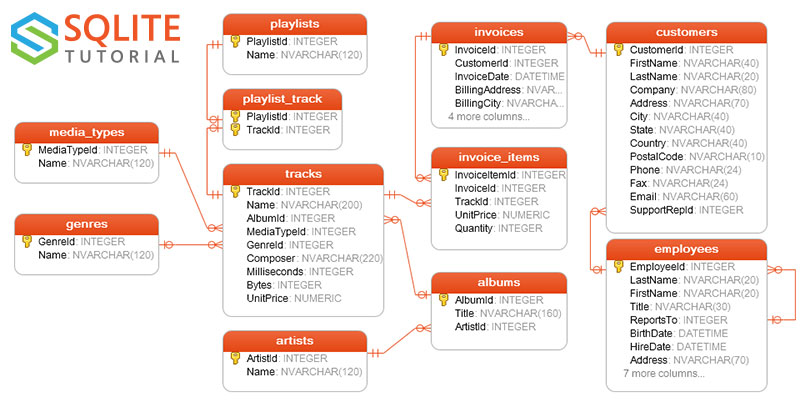
\includegraphics[width=6.25000in]{images/sqlite-sample-database-color.jpg}
\caption{}
\end{figure}

Los ejercicios pedidos en Kaggle
\href{https://www.kaggle.com/gltaboada/sqlite-tutorial-in-r}{kaggle.com/gltaboada/sqlite-tutorial-in-r}
se entregarán preferentemente antes del \textbf{14/10} compartiendo un
notebook con las soluciones (¡notebooke privado!) con el usuario
\textbf{gltaboada}. Antes me tenéis que enviar un email comunicando qué
usuario tenéis cada uno. En caso de incidencia me podéis mandar un
notebook descargado (.ipynb), o el mecanismo que hayamos acordado
previamente.

\chapter{\texorpdfstring{Manipulación de datos con
\texttt{dplyr}}{Manipulación de datos con dplyr}}\label{dplyr}

Working draft\ldots{}

En este capítulo se realiza una breve introducción al paquete
\href{https://dplyr.tidyverse.org/index.html}{\texttt{dplyr}}. Para mas
información, ver por ejemplo la `vignette' del paquete\\
\href{https://cran.rstudio.com/web/packages/dplyr/vignettes/dplyr.html}{Introduction
to dplyr}, o el Capítulo \href{http://r4ds.had.co.nz/transform.html}{5
Data transformation} del libro \href{http://r4ds.had.co.nz}{R for Data
Science}\footnote{Una alternativa (más rápida) es emplear
  \href{https://rdatatable.gitlab.io/data.table}{data.table}.}.

\section{\texorpdfstring{El paquete
\textbf{dplyr}}{El paquete dplyr}}\label{el-paquete-dplyr}

\begin{Shaded}
\begin{Highlighting}[]
\KeywordTok{library}\NormalTok{(dplyr)}
\end{Highlighting}
\end{Shaded}

\href{https://dplyr.tidyverse.org/index.html}{\texttt{dplyr}} permite
sustituir funciones base de R (como \texttt{split()}, \texttt{subset()},
\texttt{apply()}, \texttt{sapply()}, \texttt{lapply()},
\texttt{tapply()} y \texttt{aggregate()}) mediante una ``gramática'' más
sencilla para la manipulación de datos:

\begin{itemize}
\item
  \texttt{select()} seleccionar variables/columnas (también
  \texttt{rename()}).
\item
  \texttt{mutate()} crear variables/columnas (también
  \texttt{transmute()}).
\item
  \texttt{filter()} seleccionar casos/filas (también \texttt{slice()}).
\item
  \texttt{arrange()} ordenar o organizar casos/filas.
\item
  \texttt{summarise()} resumir valores.
\item
  \texttt{group\_by()} permite operaciones por grupo empleando el
  concepto ``dividir-aplicar-combinar'' (\texttt{ungroup()} elimina el
  agrupamiento).
\end{itemize}

Puede trabajar con conjuntos de datos en distintos formatos:

\begin{itemize}
\item
  \texttt{data.frame}, \texttt{data.table}, \texttt{tibble}, \ldots{}
\item
  bases de datos relacionales (lenguaje SQL); paquete
  \href{https://dbplyr.tidyverse.org}{dbplyr}, \ldots{}
\item
  bases de datos \emph{Hadoop}:

  \begin{itemize}
  \item
    \href{https://github.com/RevolutionAnalytics/plyrmr/blob/master/docs/tutorial.md}{\texttt{plyrmr}},
  \item
    \href{https://spark.rstudio.com}{\texttt{sparklyr}}
  \item
    \ldots{}
  \end{itemize}
\end{itemize}

En lugar de operar sobre vectores como las funciones base, opera sobre
objetos de este tipo (solo nos centraremos en \texttt{data.frame}).

\subsection{Datos de ejemplo}\label{datos-de-ejemplo}

El fichero \emph{empleados.RData} contiene datos de empleados de un
banco. Supongamos por ejemplo que estamos interesados en estudiar si hay
discriminación por cuestión de sexo o raza.

\section{Operaciones con variables
(columnas)}\label{operaciones-con-variables-columnas}

\subsection{\texorpdfstring{Seleccionar variables con
\textbf{select()}}{Seleccionar variables con select()}}\label{seleccionar-variables-con-select}

\begin{Shaded}
\begin{Highlighting}[]
\NormalTok{emplea2 <-}\StringTok{ }\KeywordTok{select}\NormalTok{(empleados, id, sexo, minoria, tiempemp, salini, salario)}
\KeywordTok{head}\NormalTok{(emplea2)}
\end{Highlighting}
\end{Shaded}

\begin{verbatim}
##   id   sexo minoria tiempemp salini salario
## 1  1 Hombre      No       98  27000   57000
## 2  2 Hombre      No       98  18750   40200
## 3  3  Mujer      No       98  12000   21450
## 4  4  Mujer      No       98  13200   21900
## 5  5 Hombre      No       98  21000   45000
## 6  6 Hombre      No       98  13500   32100
\end{verbatim}

Se puede cambiar el nombre (ver también \emph{?rename()})

\begin{Shaded}
\begin{Highlighting}[]
\KeywordTok{head}\NormalTok{(}\KeywordTok{select}\NormalTok{(empleados, sexo, }\DataTypeTok{noblanca =}\NormalTok{ minoria, salario))}
\end{Highlighting}
\end{Shaded}

\begin{verbatim}
##     sexo noblanca salario
## 1 Hombre       No   57000
## 2 Hombre       No   40200
## 3  Mujer       No   21450
## 4  Mujer       No   21900
## 5 Hombre       No   45000
## 6 Hombre       No   32100
\end{verbatim}

Se pueden emplear los nombres de variables como índices:

\begin{Shaded}
\begin{Highlighting}[]
\KeywordTok{head}\NormalTok{(}\KeywordTok{select}\NormalTok{(empleados, sexo}\OperatorTok{:}\NormalTok{salario))}
\end{Highlighting}
\end{Shaded}

\begin{verbatim}
##     sexo    fechnac educ         catlab salario
## 1 Hombre 1952-02-03   15      Directivo   57000
## 2 Hombre 1958-05-23   16 Administrativo   40200
## 3  Mujer 1929-07-26   12 Administrativo   21450
## 4  Mujer 1947-04-15    8 Administrativo   21900
## 5 Hombre 1955-02-09   15 Administrativo   45000
## 6 Hombre 1958-08-22   15 Administrativo   32100
\end{verbatim}

\begin{Shaded}
\begin{Highlighting}[]
\KeywordTok{head}\NormalTok{(}\KeywordTok{select}\NormalTok{(empleados, }\OperatorTok{-}\NormalTok{(sexo}\OperatorTok{:}\NormalTok{salario)))}
\end{Highlighting}
\end{Shaded}

\begin{verbatim}
##   id salini tiempemp expprev minoria     sexoraza
## 1  1  27000       98     144      No Blanca varón
## 2  2  18750       98      36      No Blanca varón
## 3  3  12000       98     381      No Blanca mujer
## 4  4  13200       98     190      No Blanca mujer
## 5  5  21000       98     138      No Blanca varón
## 6  6  13500       98      67      No Blanca varón
\end{verbatim}

Hay opciones para considerar distintos criterios:
\texttt{starts\_with()}, \texttt{ends\_with()}, \texttt{contains()},
\texttt{matches()}, \texttt{one\_of()} (ver \emph{?select}).

\begin{Shaded}
\begin{Highlighting}[]
\KeywordTok{head}\NormalTok{(}\KeywordTok{select}\NormalTok{(empleados, }\KeywordTok{starts_with}\NormalTok{(}\StringTok{"s"}\NormalTok{)))}
\end{Highlighting}
\end{Shaded}

\begin{verbatim}
##     sexo salario salini     sexoraza
## 1 Hombre   57000  27000 Blanca varón
## 2 Hombre   40200  18750 Blanca varón
## 3  Mujer   21450  12000 Blanca mujer
## 4  Mujer   21900  13200 Blanca mujer
## 5 Hombre   45000  21000 Blanca varón
## 6 Hombre   32100  13500 Blanca varón
\end{verbatim}

\subsection{\texorpdfstring{Generar nuevas variables con
\textbf{mutate()}}{Generar nuevas variables con mutate()}}\label{generar-nuevas-variables-con-mutate}

\begin{Shaded}
\begin{Highlighting}[]
\KeywordTok{head}\NormalTok{(}\KeywordTok{mutate}\NormalTok{(emplea2, }\DataTypeTok{incsal =}\NormalTok{ salario }\OperatorTok{-}\StringTok{ }\NormalTok{salini, }\DataTypeTok{tsal =}\NormalTok{ incsal}\OperatorTok{/}\NormalTok{tiempemp ))}
\end{Highlighting}
\end{Shaded}

\begin{verbatim}
##   id   sexo minoria tiempemp salini salario incsal      tsal
## 1  1 Hombre      No       98  27000   57000  30000 306.12245
## 2  2 Hombre      No       98  18750   40200  21450 218.87755
## 3  3  Mujer      No       98  12000   21450   9450  96.42857
## 4  4  Mujer      No       98  13200   21900   8700  88.77551
## 5  5 Hombre      No       98  21000   45000  24000 244.89796
## 6  6 Hombre      No       98  13500   32100  18600 189.79592
\end{verbatim}

\section{Operaciones con casos
(filas)}\label{operaciones-con-casos-filas}

\subsection{\texorpdfstring{Seleccionar casos con
\textbf{filter()}}{Seleccionar casos con filter()}}\label{seleccionar-casos-con-filter}

\begin{Shaded}
\begin{Highlighting}[]
\KeywordTok{head}\NormalTok{(}\KeywordTok{filter}\NormalTok{(emplea2, sexo }\OperatorTok{==}\StringTok{ "Mujer"}\NormalTok{, minoria }\OperatorTok{==}\StringTok{ "Sí"}\NormalTok{))}
\end{Highlighting}
\end{Shaded}

\begin{verbatim}
##   id  sexo minoria tiempemp salini salario
## 1 14 Mujer      Sí       98  16800   35100
## 2 23 Mujer      Sí       97  11100   24000
## 3 24 Mujer      Sí       97   9000   16950
## 4 25 Mujer      Sí       97   9000   21150
## 5 40 Mujer      Sí       96   9000   19200
## 6 41 Mujer      Sí       96  11550   23550
\end{verbatim}

\subsection{\texorpdfstring{Organizar casos con
\textbf{arrange()}}{Organizar casos con arrange()}}\label{organizar-casos-con-arrange}

\begin{Shaded}
\begin{Highlighting}[]
\KeywordTok{head}\NormalTok{(}\KeywordTok{arrange}\NormalTok{(emplea2, salario))}
\end{Highlighting}
\end{Shaded}

\begin{verbatim}
##    id  sexo minoria tiempemp salini salario
## 1 378 Mujer      No       70  10200   15750
## 2 338 Mujer      No       74  10200   15900
## 3  90 Mujer      No       92   9750   16200
## 4 224 Mujer      No       82  10200   16200
## 5 411 Mujer      No       68  10200   16200
## 6 448 Mujer      Sí       66  10200   16350
\end{verbatim}

\begin{Shaded}
\begin{Highlighting}[]
\KeywordTok{head}\NormalTok{(}\KeywordTok{arrange}\NormalTok{(emplea2, }\KeywordTok{desc}\NormalTok{(salini), salario))}
\end{Highlighting}
\end{Shaded}

\begin{verbatim}
##    id   sexo minoria tiempemp salini salario
## 1  29 Hombre      No       96  79980  135000
## 2 343 Hombre      No       73  60000  103500
## 3 205 Hombre      No       83  52500   66750
## 4 160 Hombre      No       86  47490   66000
## 5 431 Hombre      No       66  45000   86250
## 6  32 Hombre      No       96  45000  110625
\end{verbatim}

\section{\texorpdfstring{Resumir valores con
\textbf{summarise()}}{Resumir valores con summarise()}}\label{resumir-valores-con-summarise}

\begin{Shaded}
\begin{Highlighting}[]
\KeywordTok{summarise}\NormalTok{(empleados, }\DataTypeTok{sal.med =} \KeywordTok{mean}\NormalTok{(salario), }\DataTypeTok{n =} \KeywordTok{n}\NormalTok{())}
\end{Highlighting}
\end{Shaded}

\begin{verbatim}
##    sal.med   n
## 1 34419.57 474
\end{verbatim}

\section{\texorpdfstring{Agrupar casos con
\textbf{group\_by()}}{Agrupar casos con group\_by()}}\label{agrupar-casos-con-group_by}

\begin{Shaded}
\begin{Highlighting}[]
\KeywordTok{summarise}\NormalTok{(}\KeywordTok{group_by}\NormalTok{(empleados, sexo, minoria), }\DataTypeTok{sal.med =} \KeywordTok{mean}\NormalTok{(salario), }\DataTypeTok{n =} \KeywordTok{n}\NormalTok{())}
\end{Highlighting}
\end{Shaded}

\begin{verbatim}
## # A tibble: 4 x 4
## # Groups:   sexo [2]
##   sexo   minoria sal.med     n
##   <fct>  <fct>     <dbl> <int>
## 1 Hombre No       44475.   194
## 2 Hombre Sí       32246.    64
## 3 Mujer  No       26707.   176
## 4 Mujer  Sí       23062.    40
\end{verbatim}

\section{\texorpdfstring{Operador \emph{pipe}
\textbf{\%\textgreater{}\%} (tubería,
redirección)}{Operador pipe \%\textgreater{}\% (tubería, redirección)}}\label{operador-pipe-tuberuxeda-redirecciuxf3n}

Este operador le permite canalizar la salida de una función a la entrada
de otra función. \texttt{segundo(primero(datos))} se traduce en
\texttt{datos\ \%\textgreater{}\%\ primero\ \%\textgreater{}\%\ segundo}
(lectura de funciones de izquierda a derecha).

Ejemplos:

\begin{Shaded}
\begin{Highlighting}[]
\NormalTok{empleados }\OperatorTok\StringTok{  }\KeywordTok{filter}\NormalTok{(catlab }\OperatorTok{==}\StringTok{ "Directivo"}\NormalTok{) }\OperatorTok
\StringTok{          }\KeywordTok{group_by}\NormalTok{(sexo, minoria) }\OperatorTok
\StringTok{          }\KeywordTok{summarise}\NormalTok{(}\DataTypeTok{sal.med =} \KeywordTok{mean}\NormalTok{(salario), }\DataTypeTok{n =} \KeywordTok{n}\NormalTok{())}
\end{Highlighting}
\end{Shaded}

\begin{verbatim}
## # A tibble: 3 x 4
## # Groups:   sexo [2]
##   sexo   minoria sal.med     n
##   <fct>  <fct>     <dbl> <int>
## 1 Hombre No       65684.    70
## 2 Hombre Sí       76038.     4
## 3 Mujer  No       47214.    10
\end{verbatim}

\begin{Shaded}
\begin{Highlighting}[]
\NormalTok{empleados }\OperatorTok\StringTok{ }\KeywordTok{select}\NormalTok{(sexo, catlab, salario) }\OperatorTok
\StringTok{          }\KeywordTok{filter}\NormalTok{(catlab }\OperatorTok{!=}\StringTok{ "Seguridad"}\NormalTok{) }\OperatorTok
\StringTok{          }\KeywordTok{group_by}\NormalTok{(catlab) }\OperatorTok
\StringTok{          }\KeywordTok{mutate}\NormalTok{(}\DataTypeTok{saldif =}\NormalTok{ salario }\OperatorTok{-}\StringTok{ }\KeywordTok{mean}\NormalTok{(salario)) }\OperatorTok
\StringTok{          }\KeywordTok{ungroup}\NormalTok{() }\OperatorTok
\StringTok{          }\KeywordTok{boxplot}\NormalTok{(saldif }\OperatorTok{~}\StringTok{ }\NormalTok{sexo}\OperatorTok{*}\KeywordTok{droplevels}\NormalTok{(catlab), }\DataTypeTok{data =}\NormalTok{ .)}
\KeywordTok{abline}\NormalTok{(}\DataTypeTok{h =} \DecValTok{0}\NormalTok{, }\DataTypeTok{lty =} \DecValTok{2}\NormalTok{)}
\end{Highlighting}
\end{Shaded}

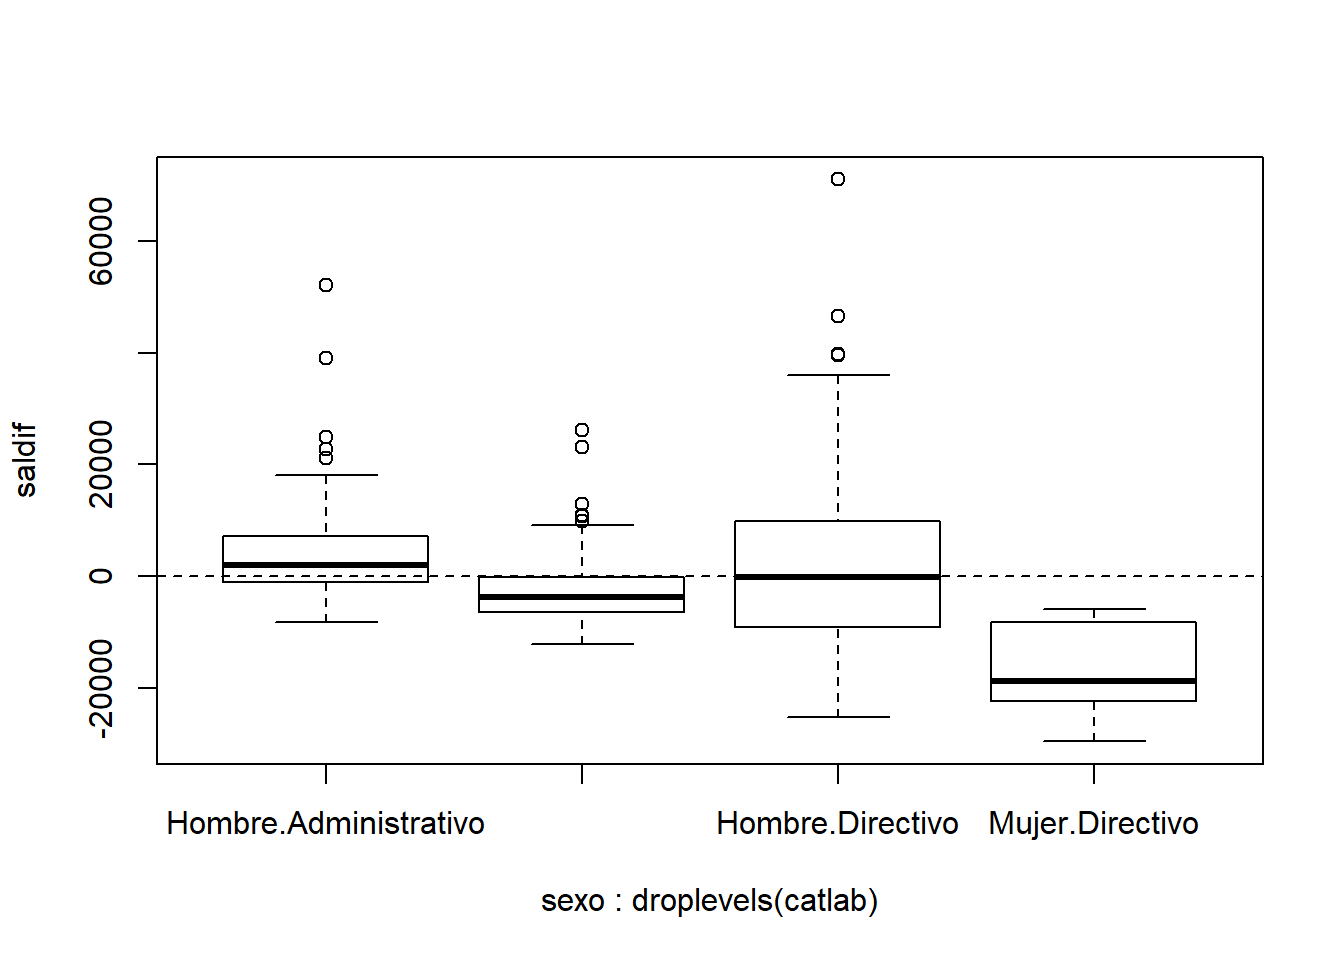
\includegraphics{04-dplyr_files/figure-latex/unnamed-chunk-12-1.pdf}

\section{Operaciones con tablas de
datos}\label{operaciones-con-tablas-de-datos-1}

Se emplean funciones \texttt{xxx\_join()} (ver la documentación del
paquete \href{https://dplyr.tidyverse.org/reference/join.html}{Join two
tbls together}, o la vignette
\href{https://dplyr.tidyverse.org/articles/two-table.html}{Two-table
verbs}):

\begin{itemize}
\item
  \texttt{inner\_join()}: devuelve las filas de \texttt{x} que tienen
  valores coincidentes en \texttt{y}, y todas las columnas de \texttt{x}
  e \texttt{y}. Si hay varias coincidencias entre \texttt{x} e
  \texttt{y}, se devuelven todas las combinaciones.
\item
  \texttt{left\_join()}: devuelve todas las filas de \texttt{x} y todas
  las columnas de \texttt{x} e \texttt{y}. Las filas de \texttt{x} sin
  correspondencia en \texttt{y} contendrán \texttt{NA} en las nuevas
  columnas. Si hay varias coincidencias entre \texttt{x} e \texttt{y},
  se devuelven todas las combinaciones (duplicando las filas).
  \texttt{right\_join()} hace lo contrario, devuelve todas las filas de
  \texttt{y}, y \texttt{full\_join()} devuelve todas las filas de
  \texttt{x} e \texttt{y} (duplicando o asignando \texttt{NA} si es
  necesario).
\item
  \texttt{semi\_join()}: devuelve las filas de \texttt{x} que tienen
  valores coincidentes en \texttt{y}, manteniendo sólo las columnas de
  \texttt{x} (al contrario que \texttt{inner\_join()} no duplica filas).
  \texttt{anti\_join()} hace lo contrario, devuelve las filas sin
  correspondencia.
\end{itemize}

El parámetro \texttt{by} determina las variables clave para las
correspondencias. Si no se establece se considerarán todas las que
tengan el mismo nombre en ambas tablas. Se puede establecer a un vector
de nombres coincidentes y en caso de que los nombres sean distintos a un
vector con nombres de la forma \texttt{c("clave\_x"\ =\ "clave\_y")}.

Adicionalmente, si las tablas \texttt{x} e \texttt{y} tienen las mismas
variables, se pueden combinar las observaciones con operaciones de
conjuntos:

\begin{itemize}
\item
  \texttt{intersect(x,\ y)}: observaciones en \texttt{x} y en
  \texttt{y}.
\item
  \texttt{union(x,\ y)}: observaciones en \texttt{x} o \texttt{y} no
  duplicadas.
\item
  \texttt{setdiff(x,\ y)}: observaciones en \texttt{x} pero no en
  \texttt{y}.
\end{itemize}

\section{Bases de datos con dplyr}\label{bases-de-datos-con-dplyr}

Algunos enlaces:

\begin{itemize}
\item
  \href{https://db.rstudio.com}{Databases using R}

  \begin{itemize}
  \item
    \href{https://db.rstudio.com/overview}{dplyr as a database
    interface}
  \item
    \href{https://db.rstudio.com/dplyr}{Databases using dplyr}
  \end{itemize}
\item
  \href{https://dbplyr.tidyverse.org/articles/dbplyr.html}{Introduction
  to dbplyr}
\item
  \href{https://datacarpentry.org/R-ecology-lesson/index.html}{Data
  Carpentry}

  \begin{itemize}
  \tightlist
  \item
    \href{https://datacarpentry.org/R-ecology-lesson/05-r-and-databases.html}{SQL
    databases and R},
  \end{itemize}
\item
  \href{https://intellixus.com/2018/06/29/r-and-data-when-should-we-use-relational-databases}{R
  and Data -- When Should we Use Relational Databases?}
\end{itemize}

\subsection{Ejemplos (Práctica 1)}\label{ejemplos-pruxe1ctica-1}

Como ejemplo emplearemos los ejercicios de la Práctica 1.

\begin{Shaded}
\begin{Highlighting}[]
\CommentTok{# install.packages('dbplyr')}
\KeywordTok{library}\NormalTok{(dplyr)}
\KeywordTok{library}\NormalTok{(dbplyr)}
\end{Highlighting}
\end{Shaded}

Conectar la base de datos:

\begin{Shaded}
\begin{Highlighting}[]
\NormalTok{chinook <-}\StringTok{ }\NormalTok{DBI}\OperatorTok{::}\KeywordTok{dbConnect}\NormalTok{(RSQLite}\OperatorTok{::}\KeywordTok{SQLite}\NormalTok{(), }\StringTok{"data/chinook.db"}\NormalTok{)}
\end{Highlighting}
\end{Shaded}

Listar tablas:

\begin{Shaded}
\begin{Highlighting}[]
\KeywordTok{src_dbi}\NormalTok{(chinook)}
\end{Highlighting}
\end{Shaded}

\begin{verbatim}
## src:  sqlite 3.30.1 [C:\Dropbox (GMODES)\__New\_MTE_TGD\tgdbook\data\chinook.db]
## tbls: albums, artists, customers, employees, genres, invoice_items, invoices,
##   media_types, playlist_track, playlists, sqlite_sequence, sqlite_stat1, tracks
\end{verbatim}

Enlazar una tabla:

\begin{Shaded}
\begin{Highlighting}[]
\NormalTok{invoices <-}\StringTok{ }\KeywordTok{tbl}\NormalTok{(chinook, }\StringTok{"invoices"}\NormalTok{)}
\NormalTok{invoices}
\end{Highlighting}
\end{Shaded}

\begin{verbatim}
## # Source:   table<invoices> [?? x 9]
## # Database: sqlite 3.30.1 [C:\Dropbox
## #   (GMODES)\__New\_MTE_TGD\tgdbook\data\chinook.db]
##    InvoiceId CustomerId InvoiceDate BillingAddress BillingCity BillingState
##        <int>      <int> <chr>       <chr>          <chr>       <chr>       
##  1         1          2 2009-01-01~ Theodor-Heuss~ Stuttgart   <NA>        
##  2         2          4 2009-01-02~ Ullevålsveien~ Oslo        <NA>        
##  3         3          8 2009-01-03~ Grétrystraat ~ Brussels    <NA>        
##  4         4         14 2009-01-06~ 8210 111 ST NW Edmonton    AB          
##  5         5         23 2009-01-11~ 69 Salem Stre~ Boston      MA          
##  6         6         37 2009-01-19~ Berger Straße~ Frankfurt   <NA>        
##  7         7         38 2009-02-01~ Barbarossastr~ Berlin      <NA>        
##  8         8         40 2009-02-01~ 8, Rue Hanovre Paris       <NA>        
##  9         9         42 2009-02-02~ 9, Place Loui~ Bordeaux    <NA>        
## 10        10         46 2009-02-03~ 3 Chatham Str~ Dublin      Dublin      
## # ... with more rows, and 3 more variables: BillingCountry <chr>,
## #   BillingPostalCode <chr>, Total <dbl>
\end{verbatim}

Ojo \texttt{{[}??\ x\ 9{]}}: de momento no conoce el número de filas.

\begin{Shaded}
\begin{Highlighting}[]
\KeywordTok{nrow}\NormalTok{(invoices)}
\end{Highlighting}
\end{Shaded}

\begin{verbatim}
## [1] NA
\end{verbatim}

Mostrar la consulta SQL:

\begin{Shaded}
\begin{Highlighting}[]
\KeywordTok{show_query}\NormalTok{(}\KeywordTok{head}\NormalTok{(invoices))}
\end{Highlighting}
\end{Shaded}

\begin{verbatim}
## <SQL>
## SELECT *
## FROM `invoices`
## LIMIT 6
\end{verbatim}

\begin{Shaded}
\begin{Highlighting}[]
\KeywordTok{str}\NormalTok{(}\KeywordTok{head}\NormalTok{(invoices))}
\end{Highlighting}
\end{Shaded}

\begin{verbatim}
## List of 2
##  $ src:List of 2
##   ..$ con  :Formal class 'SQLiteConnection' [package "RSQLite"] with 7 slots
##   .. .. ..@ ptr                :<externalptr> 
##   .. .. ..@ dbname             : chr "C:\\Dropbox (GMODES)\\__New\\_MTE_TGD\\tgdbook\\data\\chinook.db"
##   .. .. ..@ loadable.extensions: logi TRUE
##   .. .. ..@ flags              : int 70
##   .. .. ..@ vfs                : chr ""
##   .. .. ..@ ref                :<environment: 0x00000000188c2c00> 
##   .. .. ..@ bigint             : chr "integer64"
##   ..$ disco: NULL
##   ..- attr(*, "class")= chr [1:4] "src_SQLiteConnection" "src_dbi" "src_sql" "src"
##  $ ops:List of 4
##   ..$ name: chr "head"
##   ..$ x   :List of 2
##   .. ..$ x   : 'ident' chr "invoices"
##   .. ..$ vars: chr [1:9] "InvoiceId" "CustomerId" "InvoiceDate" "BillingAddress" ...
##   .. ..- attr(*, "class")= chr [1:3] "op_base_remote" "op_base" "op"
##   ..$ dots: list()
##   ..$ args:List of 1
##   .. ..$ n: num 6
##   ..- attr(*, "class")= chr [1:3] "op_head" "op_single" "op"
##  - attr(*, "class")= chr [1:5] "tbl_SQLiteConnection" "tbl_dbi" "tbl_sql" "tbl_lazy" ...
\end{verbatim}

Al trabajar con bases de datos, dplyr intenta ser lo más vago posible:

\begin{itemize}
\item
  No exporta datos a R a menos que se pida explícitamente
  (\texttt{colect()}).
\item
  Retrasa cualquier operación lo máximo posible: agrupa todo lo que se
  desea hacer y luego hace una única petición a la base de datos.
\end{itemize}

\begin{Shaded}
\begin{Highlighting}[]
\NormalTok{invoices }\OperatorTok\StringTok{ }\NormalTok{head }\OperatorTok\StringTok{ }\NormalTok{collect}
\end{Highlighting}
\end{Shaded}

\begin{verbatim}
## # A tibble: 6 x 9
##   InvoiceId CustomerId InvoiceDate BillingAddress BillingCity BillingState
##       <int>      <int> <chr>       <chr>          <chr>       <chr>       
## 1         1          2 2009-01-01~ Theodor-Heuss~ Stuttgart   <NA>        
## 2         2          4 2009-01-02~ Ullevålsveien~ Oslo        <NA>        
## 3         3          8 2009-01-03~ Grétrystraat ~ Brussels    <NA>        
## 4         4         14 2009-01-06~ 8210 111 ST NW Edmonton    AB          
## 5         5         23 2009-01-11~ 69 Salem Stre~ Boston      MA          
## 6         6         37 2009-01-19~ Berger Straße~ Frankfurt   <NA>        
## # ... with 3 more variables: BillingCountry <chr>, BillingPostalCode <chr>,
## #   Total <dbl>
\end{verbatim}

\begin{Shaded}
\begin{Highlighting}[]
\NormalTok{invoices }\OperatorTok\StringTok{ }\NormalTok{count }\CommentTok{# número de filas}
\end{Highlighting}
\end{Shaded}

\begin{verbatim}
## Warning: The `add` argument of `group_by()` is deprecated as of dplyr 1.0.0.
## Please use the `.add` argument instead.
## This warning is displayed once every 8 hours.
## Call `lifecycle::last_warnings()` to see where this warning was generated.
\end{verbatim}

\begin{verbatim}
## # Source:   lazy query [?? x 1]
## # Database: sqlite 3.30.1 [C:\Dropbox
## #   (GMODES)\__New\_MTE_TGD\tgdbook\data\chinook.db]
##       n
##   <int>
## 1   412
\end{verbatim}

\begin{enumerate}
\def\labelenumi{\arabic{enumi}.}
\item
  Conocer el importe mínimo, máximo y la media de las facturas

\begin{Shaded}
\begin{Highlighting}[]
\NormalTok{res <-}\StringTok{ }\NormalTok{invoices }\OperatorTok\StringTok{ }\KeywordTok{summarise}\NormalTok{(}\DataTypeTok{min =} \KeywordTok{min}\NormalTok{(Total, }\DataTypeTok{na.rm =} \OtherTok{TRUE}\NormalTok{), }
                        \DataTypeTok{max =} \KeywordTok{max}\NormalTok{(Total, }\DataTypeTok{na.rm =} \OtherTok{TRUE}\NormalTok{), }\DataTypeTok{med =} \KeywordTok{mean}\NormalTok{(Total, }\DataTypeTok{na.rm =} \OtherTok{TRUE}\NormalTok{))}
\KeywordTok{show_query}\NormalTok{(res)}
\end{Highlighting}
\end{Shaded}

\begin{verbatim}
## <SQL>
## SELECT MIN(`Total`) AS `min`, MAX(`Total`) AS `max`, AVG(`Total`) AS `med`
## FROM `invoices`
\end{verbatim}

\begin{Shaded}
\begin{Highlighting}[]
\NormalTok{res  }\OperatorTok\StringTok{ }\NormalTok{collect}
\end{Highlighting}
\end{Shaded}

\begin{verbatim}
## # A tibble: 1 x 3
##     min   max   med
##   <dbl> <dbl> <dbl>
## 1  0.99  25.9  5.65
\end{verbatim}
\item
  Conocer el total de las facturas de cada uno de los países.

\begin{Shaded}
\begin{Highlighting}[]
\NormalTok{res <-}\StringTok{ }\NormalTok{invoices }\OperatorTok\StringTok{ }\KeywordTok{group_by}\NormalTok{(BillingCountry) }\OperatorTok\StringTok{ }
\StringTok{          }\KeywordTok{summarise}\NormalTok{(}\DataTypeTok{n =} \KeywordTok{n}\NormalTok{(), }\DataTypeTok{total =} \KeywordTok{sum}\NormalTok{(Total, }\DataTypeTok{na.rm =} \OtherTok{TRUE}\NormalTok{))}
\KeywordTok{show_query}\NormalTok{(res)}
\end{Highlighting}
\end{Shaded}

\begin{verbatim}
## <SQL>
## SELECT `BillingCountry`, COUNT() AS `n`, SUM(`Total`) AS `total`
## FROM `invoices`
## GROUP BY `BillingCountry`
\end{verbatim}

\begin{Shaded}
\begin{Highlighting}[]
\NormalTok{res  }\OperatorTok\StringTok{ }\NormalTok{collect}
\end{Highlighting}
\end{Shaded}

\begin{verbatim}
## # A tibble: 24 x 3
##    BillingCountry     n total
##    <chr>          <int> <dbl>
##  1 Argentina          7  37.6
##  2 Australia          7  37.6
##  3 Austria            7  42.6
##  4 Belgium            7  37.6
##  5 Brazil            35 190. 
##  6 Canada            56 304. 
##  7 Chile              7  46.6
##  8 Czech Republic    14  90.2
##  9 Denmark            7  37.6
## 10 Finland            7  41.6
## # ... with 14 more rows
\end{verbatim}
\item
  Obtener el listado de países junto con su facturación media, ordenado

  \begin{enumerate}
  \def\labelenumii{(\alph{enumii})}
  \tightlist
  \item
    alfabéticamente por país
  \end{enumerate}

\begin{Shaded}
\begin{Highlighting}[]
\NormalTok{res <-}\StringTok{ }\NormalTok{invoices }\OperatorTok\StringTok{ }\KeywordTok{group_by}\NormalTok{(BillingCountry) }\OperatorTok\StringTok{ }
\StringTok{          }\KeywordTok{summarise}\NormalTok{(}\DataTypeTok{n =} \KeywordTok{n}\NormalTok{(), }\DataTypeTok{med =} \KeywordTok{mean}\NormalTok{(Total, }\DataTypeTok{na.rm =} \OtherTok{TRUE}\NormalTok{)) }\OperatorTok
\StringTok{          }\KeywordTok{arrange}\NormalTok{(BillingCountry)}
\KeywordTok{show_query}\NormalTok{(res)}
\end{Highlighting}
\end{Shaded}

\begin{verbatim}
## <SQL>
## SELECT `BillingCountry`, COUNT() AS `n`, AVG(`Total`) AS `med`
## FROM `invoices`
## GROUP BY `BillingCountry`
## ORDER BY `BillingCountry`
\end{verbatim}

\begin{Shaded}
\begin{Highlighting}[]
\NormalTok{res  }\OperatorTok\StringTok{ }\NormalTok{collect}
\end{Highlighting}
\end{Shaded}

\begin{verbatim}
## # A tibble: 24 x 3
##    BillingCountry     n   med
##    <chr>          <int> <dbl>
##  1 Argentina          7  5.37
##  2 Australia          7  5.37
##  3 Austria            7  6.09
##  4 Belgium            7  5.37
##  5 Brazil            35  5.43
##  6 Canada            56  5.43
##  7 Chile              7  6.66
##  8 Czech Republic    14  6.45
##  9 Denmark            7  5.37
## 10 Finland            7  5.95
## # ... with 14 more rows
\end{verbatim}
\end{enumerate}

\begin{enumerate}
\def\labelenumi{(\alph{enumi})}
\setcounter{enumi}{1}
\item
  decrecientemente por importe de facturación media

\begin{Shaded}
\begin{Highlighting}[]
\NormalTok{invoices }\OperatorTok\StringTok{ }\KeywordTok{group_by}\NormalTok{(BillingCountry) }\OperatorTok\StringTok{ }
\StringTok{          }\KeywordTok{summarise}\NormalTok{(}\DataTypeTok{n =} \KeywordTok{n}\NormalTok{(), }\DataTypeTok{med =} \KeywordTok{mean}\NormalTok{(Total, }\DataTypeTok{na.rm =} \OtherTok{TRUE}\NormalTok{)) }\OperatorTok
\StringTok{          }\KeywordTok{arrange}\NormalTok{(}\KeywordTok{desc}\NormalTok{(med)) }\OperatorTok\StringTok{ }\NormalTok{collect}
\end{Highlighting}
\end{Shaded}

\begin{verbatim}
## # A tibble: 24 x 3
##    BillingCountry     n   med
##    <chr>          <int> <dbl>
##  1 Chile              7  6.66
##  2 Ireland            7  6.52
##  3 Hungary            7  6.52
##  4 Czech Republic    14  6.45
##  5 Austria            7  6.09
##  6 Finland            7  5.95
##  7 Netherlands        7  5.80
##  8 India             13  5.79
##  9 USA               91  5.75
## 10 Norway             7  5.66
## # ... with 14 more rows
\end{verbatim}
\end{enumerate}

\begin{enumerate}
\def\labelenumi{\arabic{enumi}.}
\setcounter{enumi}{3}
\item
  Obtener un listado con Nombre y Apellidos de cliente y el importe de
  cada una de sus facturas (Hint: WHERE
  customer.CustomerID=invoices.CustomerID)

\begin{Shaded}
\begin{Highlighting}[]
\NormalTok{customers <-}\StringTok{ }\KeywordTok{tbl}\NormalTok{(chinook, }\StringTok{"customers"}\NormalTok{)}
\KeywordTok{tbl_vars}\NormalTok{(customers) }
\end{Highlighting}
\end{Shaded}

\begin{verbatim}
## <dplyr:::vars>
##  [1] "CustomerId"   "FirstName"    "LastName"     "Company"      "Address"     
##  [6] "City"         "State"        "Country"      "PostalCode"   "Phone"       
## [11] "Fax"          "Email"        "SupportRepId"
\end{verbatim}

\begin{Shaded}
\begin{Highlighting}[]
\NormalTok{res <-}\StringTok{ }\NormalTok{customers }\OperatorTok\StringTok{ }\KeywordTok{inner_join}\NormalTok{(invoices, }\DataTypeTok{by =} \StringTok{"CustomerId"}\NormalTok{) }\OperatorTok\StringTok{ }\KeywordTok{select}\NormalTok{(FirstName, LastName, Country, Total) }
\KeywordTok{show_query}\NormalTok{(res)}
\end{Highlighting}
\end{Shaded}

\begin{verbatim}
## <SQL>
## SELECT `FirstName`, `LastName`, `Country`, `Total`
## FROM (SELECT `LHS`.`CustomerId` AS `CustomerId`, `LHS`.`FirstName` AS `FirstName`, `LHS`.`LastName` AS `LastName`, `LHS`.`Company` AS `Company`, `LHS`.`Address` AS `Address`, `LHS`.`City` AS `City`, `LHS`.`State` AS `State`, `LHS`.`Country` AS `Country`, `LHS`.`PostalCode` AS `PostalCode`, `LHS`.`Phone` AS `Phone`, `LHS`.`Fax` AS `Fax`, `LHS`.`Email` AS `Email`, `LHS`.`SupportRepId` AS `SupportRepId`, `RHS`.`InvoiceId` AS `InvoiceId`, `RHS`.`InvoiceDate` AS `InvoiceDate`, `RHS`.`BillingAddress` AS `BillingAddress`, `RHS`.`BillingCity` AS `BillingCity`, `RHS`.`BillingState` AS `BillingState`, `RHS`.`BillingCountry` AS `BillingCountry`, `RHS`.`BillingPostalCode` AS `BillingPostalCode`, `RHS`.`Total` AS `Total`
## FROM `customers` AS `LHS`
## INNER JOIN `invoices` AS `RHS`
## ON (`LHS`.`CustomerId` = `RHS`.`CustomerId`)
## )
\end{verbatim}

\begin{Shaded}
\begin{Highlighting}[]
\NormalTok{res  }\OperatorTok\StringTok{ }\NormalTok{collect}
\end{Highlighting}
\end{Shaded}

\begin{verbatim}
## # A tibble: 412 x 4
##    FirstName LastName  Country Total
##    <chr>     <chr>     <chr>   <dbl>
##  1 Luís      Gonçalves Brazil   3.98
##  2 Luís      Gonçalves Brazil   3.96
##  3 Luís      Gonçalves Brazil   5.94
##  4 Luís      Gonçalves Brazil   0.99
##  5 Luís      Gonçalves Brazil   1.98
##  6 Luís      Gonçalves Brazil  13.9 
##  7 Luís      Gonçalves Brazil   8.91
##  8 Leonie    Köhler    Germany  1.98
##  9 Leonie    Köhler    Germany 13.9 
## 10 Leonie    Köhler    Germany  8.91
## # ... with 402 more rows
\end{verbatim}
\item
  ¿Qué porcentaje de las canciones son video?

\begin{Shaded}
\begin{Highlighting}[]
\NormalTok{tracks <-}\StringTok{ }\KeywordTok{tbl}\NormalTok{(chinook, }\StringTok{"tracks"}\NormalTok{)}
\KeywordTok{head}\NormalTok{(tracks) }
\end{Highlighting}
\end{Shaded}

\begin{verbatim}
## # Source:   lazy query [?? x 9]
## # Database: sqlite 3.30.1 [C:\Dropbox
## #   (GMODES)\__New\_MTE_TGD\tgdbook\data\chinook.db]
##   TrackId Name  AlbumId MediaTypeId GenreId Composer Milliseconds  Bytes
##     <int> <chr>   <int>       <int>   <int> <chr>           <int>  <int>
## 1       1 For ~       1           1       1 Angus Y~       343719 1.12e7
## 2       2 Ball~       2           2       1 <NA>           342562 5.51e6
## 3       3 Fast~       3           2       1 F. Balt~       230619 3.99e6
## 4       4 Rest~       3           2       1 F. Balt~       252051 4.33e6
## 5       5 Prin~       3           2       1 Deaffy ~       375418 6.29e6
## 6       6 Put ~       1           1       1 Angus Y~       205662 6.71e6
## # ... with 1 more variable: UnitPrice <dbl>
\end{verbatim}

\begin{Shaded}
\begin{Highlighting}[]
\NormalTok{tracks }\OperatorTok\StringTok{ }\KeywordTok{group_by}\NormalTok{(MediaTypeId) }\OperatorTok\StringTok{ }
\StringTok{    }\KeywordTok{summarise}\NormalTok{(}\DataTypeTok{n =} \KeywordTok{n}\NormalTok{()) }\OperatorTok\StringTok{ }\NormalTok{collect }\OperatorTok\StringTok{ }\KeywordTok{mutate}\NormalTok{(}\DataTypeTok{freq =}\NormalTok{ n }\OperatorTok{/}\StringTok{ }\KeywordTok{sum}\NormalTok{(n))}
\end{Highlighting}
\end{Shaded}

\begin{verbatim}
## # A tibble: 5 x 3
##   MediaTypeId     n    freq
##         <int> <int>   <dbl>
## 1           1  3034 0.866  
## 2           2   237 0.0677 
## 3           3   214 0.0611 
## 4           4     7 0.00200
## 5           5    11 0.00314
\end{verbatim}

\begin{Shaded}
\begin{Highlighting}[]
\NormalTok{media_types <-}\StringTok{ }\KeywordTok{tbl}\NormalTok{(chinook, }\StringTok{"media_types"}\NormalTok{)}
\KeywordTok{head}\NormalTok{(media_types)}
\end{Highlighting}
\end{Shaded}

\begin{verbatim}
## # Source:   lazy query [?? x 2]
## # Database: sqlite 3.30.1 [C:\Dropbox
## #   (GMODES)\__New\_MTE_TGD\tgdbook\data\chinook.db]
##   MediaTypeId Name                       
##         <int> <chr>                      
## 1           1 MPEG audio file            
## 2           2 Protected AAC audio file   
## 3           3 Protected MPEG-4 video file
## 4           4 Purchased AAC audio file   
## 5           5 AAC audio file
\end{verbatim}

\begin{Shaded}
\begin{Highlighting}[]
\NormalTok{tracks }\OperatorTok\StringTok{ }\KeywordTok{inner_join}\NormalTok{(media_types, }\DataTypeTok{by =} \StringTok{"MediaTypeId"}\NormalTok{) }\OperatorTok\StringTok{ }\KeywordTok{count}\NormalTok{(Name.y) }\OperatorTok\StringTok{ }
\StringTok{    }\NormalTok{collect }\OperatorTok\StringTok{ }\KeywordTok{mutate}\NormalTok{(}\DataTypeTok{freq =}\NormalTok{ n }\OperatorTok{/}\StringTok{ }\KeywordTok{sum}\NormalTok{(n)) }\OperatorTok\StringTok{ }\KeywordTok{filter}\NormalTok{(}\KeywordTok{grepl}\NormalTok{(}\StringTok{'video'}\NormalTok{, Name.y))}
\end{Highlighting}
\end{Shaded}

\begin{verbatim}
## # A tibble: 1 x 3
##   Name.y                          n   freq
##   <chr>                       <int>  <dbl>
## 1 Protected MPEG-4 video file   214 0.0611
\end{verbatim}
\item
  Listar los 10 mejores clientes (aquellos a los que se les ha facturado
  más cantidad) indicando Nombre, Apellidos, Pais y el importe total de
  su facturación.

\begin{Shaded}
\begin{Highlighting}[]
\NormalTok{customers }\OperatorTok\StringTok{ }\KeywordTok{inner_join}\NormalTok{(invoices, }\DataTypeTok{by =} \StringTok{"CustomerId"}\NormalTok{) }\OperatorTok\StringTok{ }\KeywordTok{group_by}\NormalTok{(CustomerId) }\OperatorTok\StringTok{ }
\StringTok{    }\KeywordTok{summarise}\NormalTok{(FirstName, LastName, country, }\DataTypeTok{total =} \KeywordTok{sum}\NormalTok{(Total, }\DataTypeTok{na.rm =} \OtherTok{TRUE}\NormalTok{)) }\OperatorTok\StringTok{  }
\StringTok{    }\KeywordTok{arrange}\NormalTok{(}\KeywordTok{desc}\NormalTok{(total)) }\OperatorTok\StringTok{ }\KeywordTok{head}\NormalTok{(}\DecValTok{10}\NormalTok{) }\OperatorTok\StringTok{ }\NormalTok{collect}
\end{Highlighting}
\end{Shaded}

\begin{verbatim}
## # A tibble: 10 x 5
##    CustomerId FirstName LastName   Country        total
##         <int> <chr>     <chr>      <chr>          <dbl>
##  1          6 Helena    Holý       Czech Republic  49.6
##  2         26 Richard   Cunningham USA             47.6
##  3         57 Luis      Rojas      Chile           46.6
##  4         45 Ladislav  Kovács     Hungary         45.6
##  5         46 Hugh      O'Reilly   Ireland         45.6
##  6         28 Julia     Barnett    USA             43.6
##  7         24 Frank     Ralston    USA             43.6
##  8         37 Fynn      Zimmermann Germany         43.6
##  9          7 Astrid    Gruber     Austria         42.6
## 10         25 Victor    Stevens    USA             42.6
\end{verbatim}
\item
  Listar los géneros musicales por orden decreciente de popularidad
  (definida la popularidad como el número de canciones de ese género),
  indicando el porcentaje de las canciones de ese género.

\begin{Shaded}
\begin{Highlighting}[]
\NormalTok{tracks }\OperatorTok\StringTok{ }\KeywordTok{inner_join}\NormalTok{(}\KeywordTok{tbl}\NormalTok{(chinook, }\StringTok{"genres"}\NormalTok{), }\DataTypeTok{by =} \StringTok{"GenreId"}\NormalTok{) }\OperatorTok\StringTok{ }\KeywordTok{count}\NormalTok{(Name.y) }\OperatorTok\StringTok{ }
\StringTok{    }\KeywordTok{arrange}\NormalTok{(}\KeywordTok{desc}\NormalTok{(n)) }\OperatorTok\StringTok{ }\NormalTok{collect }\OperatorTok\StringTok{ }\KeywordTok{mutate}\NormalTok{(}\DataTypeTok{freq =}\NormalTok{ n }\OperatorTok{/}\StringTok{ }\KeywordTok{sum}\NormalTok{(n))}
\end{Highlighting}
\end{Shaded}

\begin{verbatim}
## # A tibble: 25 x 3
##    Name.y                 n   freq
##    <chr>              <int>  <dbl>
##  1 Rock                1297 0.370 
##  2 Latin                579 0.165 
##  3 Metal                374 0.107 
##  4 Alternative & Punk   332 0.0948
##  5 Jazz                 130 0.0371
##  6 TV Shows              93 0.0265
##  7 Blues                 81 0.0231
##  8 Classical             74 0.0211
##  9 Drama                 64 0.0183
## 10 R&B/Soul              61 0.0174
## # ... with 15 more rows
\end{verbatim}
\item
  Listar los 10 artistas con mayor número de canciones de forma
  descendente según el número de canciones.

\begin{Shaded}
\begin{Highlighting}[]
\NormalTok{tracks }\OperatorTok\StringTok{ }\KeywordTok{inner_join}\NormalTok{(}\KeywordTok{tbl}\NormalTok{(chinook, }\StringTok{"albums"}\NormalTok{), }\DataTypeTok{by =} \StringTok{"AlbumId"}\NormalTok{) }\OperatorTok\StringTok{ }
\StringTok{    }\KeywordTok{inner_join}\NormalTok{(}\KeywordTok{tbl}\NormalTok{(chinook, }\StringTok{"artists"}\NormalTok{), }\DataTypeTok{by =} \StringTok{"ArtistId"}\NormalTok{) }\OperatorTok\StringTok{ }
\StringTok{    }\KeywordTok{count}\NormalTok{(Name.y) }\OperatorTok\StringTok{ }\KeywordTok{arrange}\NormalTok{(}\KeywordTok{desc}\NormalTok{(n)) }\OperatorTok\StringTok{ }\NormalTok{collect}
\end{Highlighting}
\end{Shaded}

\begin{verbatim}
## # A tibble: 204 x 2
##    Name.y              n
##    <chr>           <int>
##  1 Iron Maiden       213
##  2 U2                135
##  3 Led Zeppelin      114
##  4 Metallica         112
##  5 Lost               92
##  6 Deep Purple        92
##  7 Pearl Jam          67
##  8 Lenny Kravitz      57
##  9 Various Artists    56
## 10 The Office         53
## # ... with 194 more rows
\end{verbatim}
\end{enumerate}

Desconectar la base de datos:

\begin{Shaded}
\begin{Highlighting}[]
\NormalTok{DBI}\OperatorTok{::}\KeywordTok{dbDisconnect}\NormalTok{(chinook)            }
\end{Highlighting}
\end{Shaded}

\chapter{Introducción a Tecnologías
NoSQL}\label{introducciuxf3n-a-tecnologuxedas-nosql}

Working draft\ldots{}

\section{Conceptos y tipos de bases de datos NoSQL (documental,
columnar, clave/valor y de
grafos)}\label{conceptos-y-tipos-de-bases-de-datos-nosql-documental-columnar-clavevalor-y-de-grafos}

NoSQL - ``Not Only SQL'' - es una nueva categoría de bases de datos
no-relacionales y altamente distribuidas.

Las bases de datos NoSQL nacen de la necesidad de:

\begin{itemize}
\item
  Simplicidad en los diseños
\item
  Escalado horizontal
\item
  Mayor control en la disponibilidad
\end{itemize}

Pero cuidado, en muchos escenarios las BBDD relacionales siguen siendo
la mejor opción.

\subsection{Características de las bases de datos
NoSQL}\label{caracteruxedsticas-de-las-bases-de-datos-nosql}

\begin{itemize}
\tightlist
\item
  Libre de esquemas -- no se diseñan las tablas y relaciones por
  adelantado, además de permitir la migración del esquema.
\item
  Proporcionan replicación a través de escalado horizontal.
\item
  Este escalado horizontal se traduce en arquitectura distribuida
\item
  Generalmente ofrecen consistencia débil
\item
  Hacen uso de estructuras de datos sencillas, normalmente pares
  clave/valor a bajo nivel
\item
  Suelen tener un sistema de consultas propio (o SQL-like)
\item
  Siguen el modelo BASE (\emph{B}asic Availability, Soft state, Eventual
  consistency) en lugar de ACID (\emph{A}tomicity, \emph{C}onsistency,
  \emph{I}solation, \emph{D}urability)
\end{itemize}

El modelo BASE consiste en:

\begin{itemize}
\tightlist
\item
  Basic Availability -- el sistema garantiza disponibilidad, en términos
  del teorema CAP.
\item
  Soft state -- el estado del sistema puede cambiar a lo largo del
  tiempo, incluso sin entrada. Esto es provocado por el modelo de
  consistencia eventual.
\item
  Eventual consistency -- el sistema alcanzará un estado consistente con
  el tiempo, siempre y cuando no reciba entrada durante ese tiempo.
\end{itemize}

\subsubsection{Teorema CAP}\label{teorema-cap}

Es imposible para un sistema de cómputo distribuido garantizar
simultáneamente:

\begin{itemize}
\tightlist
\item
  Consistency -- Todos los nodos ven los mismos datos al mismo tiempo
\item
  Availability -- Toda petición obtiene una respuesta en caso tanto de
  éxito como fallo
\item
  Partition Tolerance -- El sistema seguirá funcionando ante pérdidas
  arbitrarias de información o fallos parciales
\end{itemize}

\begin{figure}
\centering
\includegraphics{images/TeoremaCAP.jpg}
\caption{}
\end{figure}

Las razones para escoger NoSQL son:

\begin{itemize}
\tightlist
\item
  Analítica
\item
  Gran cantidad de escrituras, análisis en bloque
\item
  Escalabilidad
\item
  Tan fácil como añadir un nuevo nodo a la red, bajo coste.
\item
  Redundancia
\item
  Están diseñadas teniendo en cuenta la redundancia
\item
  Rápido desarrollo
\item
  Al ser schema-less o schema on-read son más flexibles que schema
  on-write
\item
  Flexibilidad en el almacenamiento de datos
\item
  Almacenan todo tipo de datos: texto, imágenes, BLOBs
\item
  Gran rendimiento en consultas sobre datos que no implican relaciones
  jerárquicas
\item
  Gran rendimiento sobre BBDD desnormalizadas
\item
  Tamaño
\item
  El tamaño del esquema de datos es demasiado grande
\item
  Muchos datos temporales fuera de almacén principal
\end{itemize}

Razones para NO escoger NoSQL: * Consistencia y Disponibilidad de los
datos son críticas * Relaciones entre datos son importantes + E.g. joins
numerosos y/o importantes * En general, cuando el modelo ACID encaja
mejor

\subsection{Tipos de Bases de Datos
NoSQL}\label{tipos-de-bases-de-datos-nosql}

\begin{figure}
\centering
\includegraphics{images/TiposBBDDNoSQL.png}
\caption{}
\end{figure}

\begin{figure}
\centering
\includegraphics{images/TiposBBDDNoSQL2.png}
\caption{}
\end{figure}

\begin{figure}
\centering
\includegraphics{images/451ResearchMap.png}
\caption{}
\end{figure}

\begin{figure}
\centering
\includegraphics{images/DBEnginesRanking.png}
\caption{}
\end{figure}

\begin{figure}
\centering
\includegraphics{images/451ResearchSkills.png}
\caption{}
\end{figure}

\subsection{MongoDB: NoSQL documental}\label{mongodb-nosql-documental}

\begin{figure}
\centering
\includegraphics{images/MongoDB.jpg}
\caption{}
\end{figure}

\subsection{Redis: NoSQL key-value}\label{redis-nosql-key-value}

In-memory data structure store, útil para base de datos de
login-password, sensor-valor, URL-respuesta, con una sintaxis muy
sencilla:

\begin{itemize}
\tightlist
\item
  El comando SET almacena valores
\item
  SET server:name ``luna''
\item
  Recuperamos esos valores con GET
\item
  GET server:name
\item
  INCR incrementa atómicamente un valor
\item
  INCR clients
\item
  DEL elimina claves y sus valores asociados
\item
  DEL clients
\item
  TTL (Time To Live) útil para cachés
\item
  EXPIRE promocion 60
\end{itemize}

\subsection{Cassandra: NoSQL columnar}\label{cassandra-nosql-columnar}

\begin{figure}
\centering
\includegraphics{images/BlogRDMS.png}
\caption{}
\end{figure}

\begin{figure}
\centering
\includegraphics{images/BlogNoSQL.png}
\caption{}
\end{figure}

\subsection{Neo4j: NoSQL grafos}\label{neo4j-nosql-grafos}

\begin{figure}
\centering
\includegraphics{images/Neo4jlogo.png}
\caption{}
\end{figure}

\begin{figure}
\centering
\includegraphics{images/CypherQuery.png}
\caption{}
\end{figure}

\begin{figure}
\centering
\includegraphics{images/CypherResult.png}
\caption{}
\end{figure}

\subsection{Otros: search engines}\label{otros-search-engines}

Son sistemas especializados en búsquedas, procesamiento de lenguaje
natural como ElasticSearch, Solr, Splunk (logs de aplicaciones),
etc\ldots{}

\section{Conexión de R a MongoDB}\label{conexiuxf3n-de-r-a-mongodb}

A través del paquete
\href{https://cran.rstudio.com/web/packages/mongolite/mongolite.pdf}{mongolite},
aquí tenéis un
\href{https://datascienceplus.com/using-mongodb-with-r/}{Tutorial}

\begin{Shaded}
\begin{Highlighting}[]
\KeywordTok{install.packages}\NormalTok{(}\StringTok{"mongolite"}\NormalTok{)}
\end{Highlighting}
\end{Shaded}

\begin{Shaded}
\begin{Highlighting}[]
\KeywordTok{library}\NormalTok{(mongolite)}

\CommentTok{# Connect to a local MongoDB}

\NormalTok{my_collection =}\StringTok{ }\KeywordTok{mongo}\NormalTok{(}\DataTypeTok{collection =} \StringTok{"restaurants"}\NormalTok{, }\DataTypeTok{db =} \StringTok{"Restaurants"}\NormalTok{) }\CommentTok{# create connection, database and collection}
\NormalTok{my_collection}\OperatorTok{$}\NormalTok{count}
\end{Highlighting}
\end{Shaded}

\section{Práctica 2: NoSQL}\label{pruxe1ctica-2-nosql}

Los ejercicios se entregarán por correo electrónico a
\href{mailto:guillermo.lopez.taboada@udc.es}{\nolinkurl{guillermo.lopez.taboada@udc.es}}
en formato R MarkDown con el nombre de archivo P1-Nombre-Apellidos.Rmd
(sin tildes ni caracteres especiales en el nombre del arhivo)
\textbf{antes} del 20 de Noviembre.

\subsection{Ejercicios con RMongolite}\label{ejercicios-con-rmongolite}

Realizaremos una serie de ejercicios con la collección {[}Restaurants{]}
(\url{https://www.w3resource.com/mongodb-exercises/restaurants.zip})
importados mediante:

\begin{Shaded}
\begin{Highlighting}[]
\CommentTok{# En Windows}
\NormalTok{mongoimport.exe }\OperatorTok{--}\NormalTok{db=Restaurants }\OperatorTok{--}\NormalTok{file=D}\OperatorTok{:}\NormalTok{\textbackslash{}DATA\textbackslash{}opendata\textbackslash{}restaurants.json}
\end{Highlighting}
\end{Shaded}

La puntuación de esta práctica será el número de respuestas correctas:

\begin{enumerate}
\def\labelenumi{\arabic{enumi}.}
\item
  Mostrar todos los documentos de la colección restaurants (que no se
  ejecute en el .rmd, sólo la query)
\item
  Mostrar nombre de restaurante, barrio y cocina de la colección
  restaurants (que no se ejecute en el .rmd, sólo la query)
\item
  Mostrar los primeros 5 restaurantes del barrio Bronx.
\item
  Mostrar los restaurantes con una longitud menor que -75.7541
\item
  Mostrar los restaurantes con una puntuación superior a 90
\item
  Mostrar los restaurantes de comida American o Chineese del barrio
  Queens.
\item
  Mostrar los restaurantes con un grado ``A'' y puntuación 9 obtenida en
  fecha 2014-08-11T00:00:00Z
\item
  Con valor de 3 puntos, propón un JSON para descargar, indícame la URL,
  si has de hacer algún proceso antes de importarlo en MongoDB, cómo lo
  importas, dame un pantallazo del análisis exploratorio de ese JSON y
  una query que harías contra ese JSON (la query en MongoDB, Compass o
  RmongoDB)
\end{enumerate}

\chapter{Tecnologías para el Tratamiendo de Datos
Masivos}\label{tecnologuxedas-para-el-tratamiendo-de-datos-masivos}

En este tema vamos a ver las tecnologías más relevantes para el
tratamiento de datos masivos dentro de R, como son Spark (con sparklyr)
dentro del ecosistema Hadoop. Los ejercicios prácticos se realizarán
sobre la \href{http://bigdata.cesga.es/}{plataforma Big Data} del
\href{http://www.cesga.es}{Centro de Supercomputación de Galicia
(CESGA)}

\begin{figure}
\centering
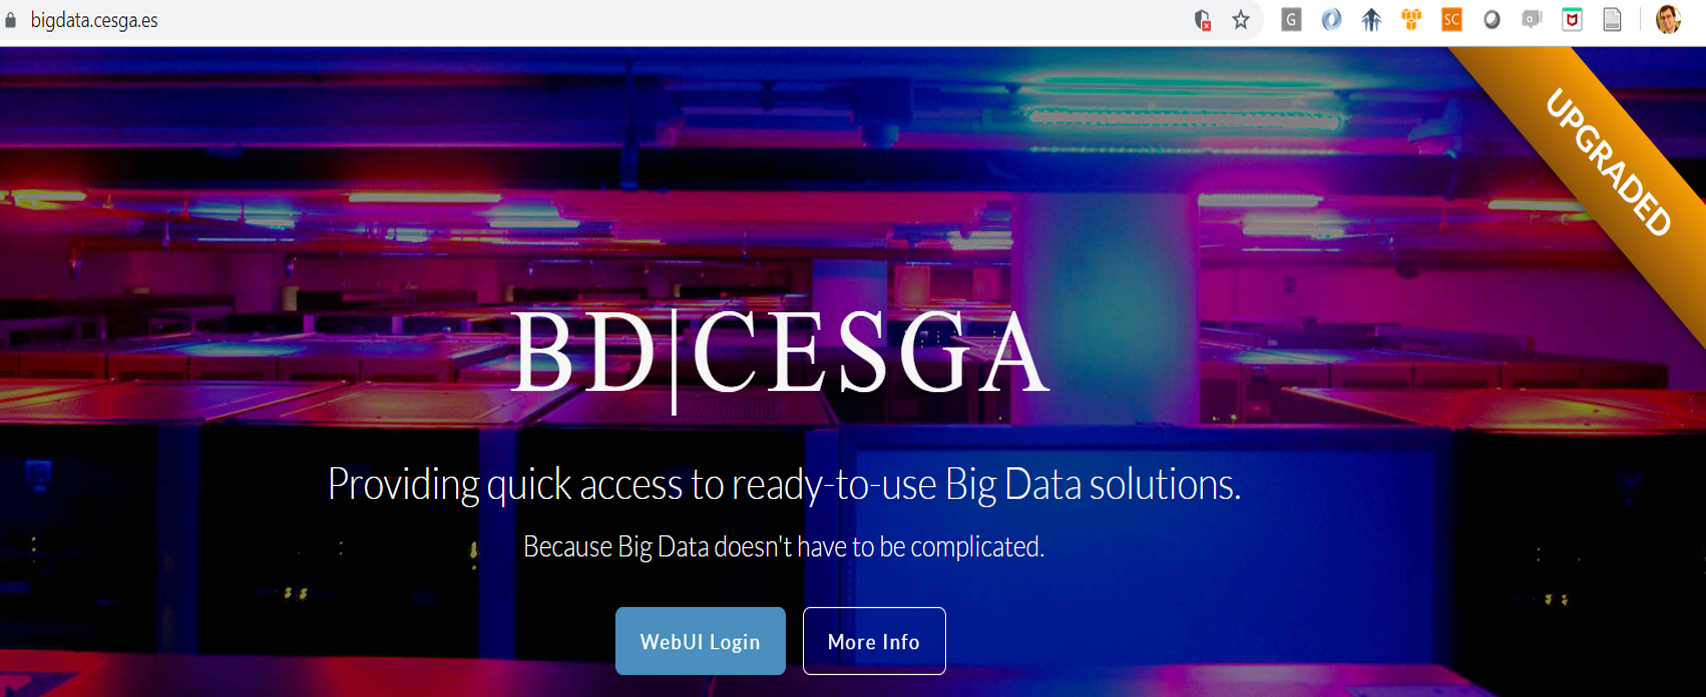
\includegraphics{images/T3-bigdatacesga.png}
\caption{}
\end{figure}

\section{Tecnologías Big Data (Hadoop, Spark, Hive, Rspark,
Sparklyr)}\label{tecnologuxedas-big-data-hadoop-spark-hive-rspark-sparklyr}

A continuación se introducen los conceptos básicos de las tecnologías
Big Data:

\begin{itemize}
\item
  Hadoop: framework open-source desarrollado en Java principalmente que
  soporta aplicaciones distribuidas sobre miles de nodos y a escala
  Petabyte. Está inspierado en el diseño de las operaciones de MapReduce
  de Google y el Google File System (GFS). Entre sus principales
  componentes destaca HDFS Hadoop Distributed File System, sistema de
  ficheros distribuido sobre múltiples nodos y accesible a nivel de
  aplicación. También destaca YARN como gestor de recursos, para
  ejecutar aplicaciones. Destacar que la versión original, Hadoop 1,
  estaba basada extensivamente en Map Reduce, Hadoop 2 colocó en su core
  a YARN y Hadoop 3 está orientado a la provisión de Plataforma como
  servicio y ejecución simultánea de múltiples cargas de trabajo
  distribuidas sobre recursos solicitados bajo demanda.
\item
  Hive: es un sistema de almancenamiento y explotación de datos del
  estilo de un data warehouse open source diseñado para ser ejecutado en
  entornos Hadoop. Permite agrupar, consultar y analizar datos
  almacenados en Hadoop File System y en Amazon S3 (almacenamiento de
  objetos en general) en esquema en estrella. Su lenguaje de consulta de
  datos, Hive Query Language o (HQL).
\item
  Spark: framework de computación distribuida open-source para el
  procesamiento de datos masivos sobre Hadoop con un paralelismo
  implícito sobre su estructura de datos (Resilient Distributed Dataset
  o RDD), permite operar en paralelo sobre una colección de datos sin
  saber en qué servidores están disponibles dichos datos y de una forma
  tolerante a fallos. Es uno de los principales frameworks de
  programación de entornos Hadoop al estar optimizado su procesamiento
  sobre memoria (en lugar de sobre archivos en disco) para obtener
  velocidad, tanto en sus vertientes Spark streaming y Spark SQL, como
  Spark Machile Learning MLlib. Dispone de interfaces en Java, Scala,
  Python y R, siendo las interfaces de R Rspark y Sparklyr.
\item
  SparkR: es un paquete, el primero que apareció, para conectar R con
  Spark. Intenta ser lo más parecida a la interfaz estándard de R de
  manipulación de datos.
\item
  Sparklyr: es una librería para conectar R con Spark posterior a
  SparkR. Intenta ser lo más parecida a dplyr y embeber SQL en las
  consultas, soportando una mayor cantidad de paquetes. Por este motivo
  es el proyecto más activo actualmente, sustituyendo a SparkR.
\end{itemize}

\begin{figure}
\centering
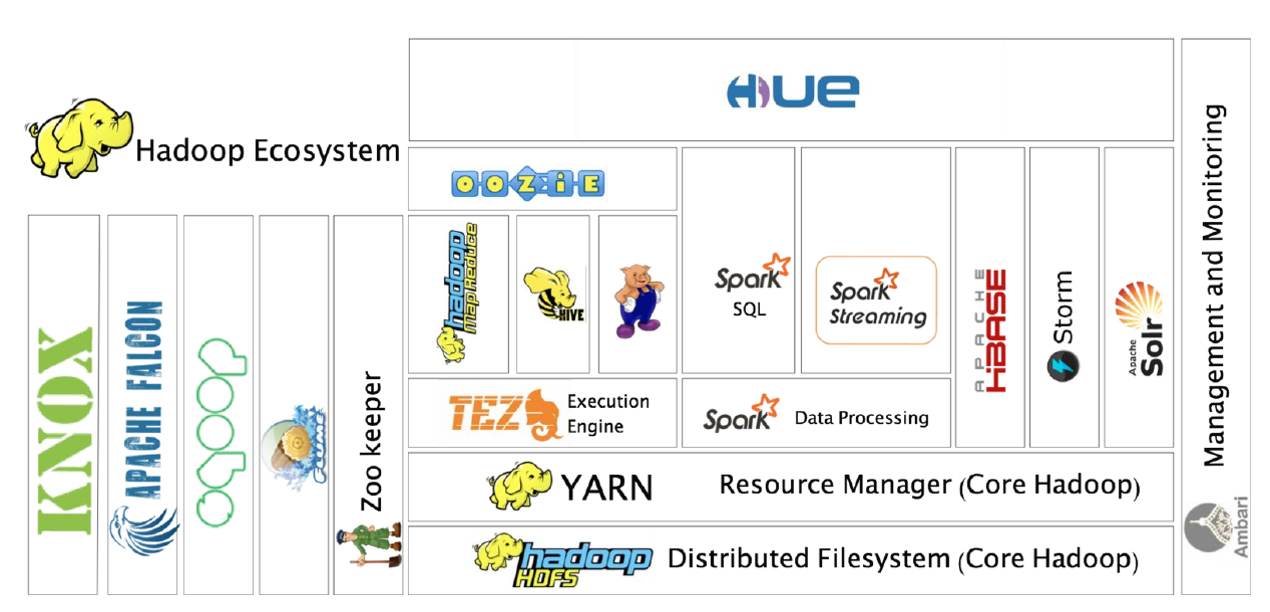
\includegraphics{images/T3-ecosistema.png}
\caption{}
\end{figure}

\subsection{Uso de Hadoop con dos
ejemplos:}\label{uso-de-hadoop-con-dos-ejemplos}

Conexión vía SSH a CESGA (siempre con VPN activada!) y ejemplo \#1:

\begin{Shaded}
\begin{Highlighting}[]
\NormalTok{wget  https}\OperatorTok{:}\ErrorTok{//}\NormalTok{packages.revolutionanalytics.com}\OperatorTok{/}\NormalTok{datasets}\OperatorTok{/}\NormalTok{claims2.csv }

\CommentTok{# [3 minutos – 1GB/minuto en CESGA]  [recomendada la descarga desde servidor dtn.srv.cesga.es] [copia temp /tmp]}

\NormalTok{hadoop fs –mkdir p1}\OperatorTok{/}
\NormalTok{hadoop fs }\OperatorTok{-}\NormalTok{mkdir p1}\OperatorTok{/}\NormalTok{claims}\OperatorTok{/}
\NormalTok{hadoop fs –put claims2.csv p1}\OperatorTok{/}\NormalTok{claims}\OperatorTok{/}\StringTok{   }\NormalTok{[}\DecValTok{3}\NormalTok{ segundos]}
\NormalTok{hadoop fs –ls p1}\OperatorTok{/}\NormalTok{claims}\OperatorTok{/}

\ErrorTok{$}\StringTok{ }\NormalTok{myquota}
\CommentTok{# [1TB en $HOMEBD y 18TB en Hadoop]}

\OperatorTok{$}\StringTok{ }\NormalTok{spark}\OperatorTok{-}\NormalTok{shell }\OperatorTok{--}\NormalTok{packages com.databricks}\OperatorTok{:}\NormalTok{spark}\OperatorTok{-}\NormalTok{csv_}\FloatTok{2.10}\OperatorTok{:}\FloatTok{1.4}\NormalTok{.}\DecValTok{0}
\OperatorTok{>}\StringTok{ }\NormalTok{val sqlContext =}\StringTok{ }\NormalTok{new }\KeywordTok{org.apache.spark.sql.SQLContext}\NormalTok{(sc); }
\OperatorTok{>}\StringTok{ }\NormalTok{val df =}\StringTok{ }\KeywordTok{sqlContext.read.format}\NormalTok{(csv)}\KeywordTok{.option}\NormalTok{(header, true)}\KeywordTok{.load}\NormalTok{(p1}\OperatorTok{/}\NormalTok{claims}\OperatorTok{/}\NormalTok{claims2.csv)}
\OperatorTok{>}\StringTok{ }\KeywordTok{df.count}\NormalTok{();  }\KeywordTok{df.first}\NormalTok{();  }\KeywordTok{df.take}\NormalTok{(}\DecValTok{5}\NormalTok{);  }\KeywordTok{df.printSchema}\NormalTok{();}
\OperatorTok{>}\StringTok{ }\KeywordTok{df.registerTempTable}\NormalTok{(TblName)}
\OperatorTok{>}\StringTok{ }\KeywordTok{sqlContext.sql}\NormalTok{(select }\OperatorTok{*}\StringTok{ }\NormalTok{from TblName limit }\DecValTok{100}\NormalTok{)}\KeywordTok{.take}\NormalTok{(}\DecValTok{100}\NormalTok{)}\KeywordTok{.foreach}\NormalTok{(println)}
\OperatorTok{>}\StringTok{ }\KeywordTok{sqlContext.sql}\NormalTok{(select }\OperatorTok{*}\StringTok{ }\NormalTok{from TblName where }\DataTypeTok{Calendar_year=}\DecValTok{2005}\NormalTok{)}\KeywordTok{.count}\NormalTok{()}
\end{Highlighting}
\end{Shaded}

Usando Spark-shell pero también podemos realizar ciertos análisis con
hive:

\begin{Shaded}
\begin{Highlighting}[]
\OperatorTok{$}\StringTok{ }\NormalTok{hadoop fs }\OperatorTok{-}\NormalTok{mkdir bdp}
\OperatorTok{$}\StringTok{ }\NormalTok{hadoop fs }\OperatorTok{-}\NormalTok{mkdir bdp}\OperatorTok{/}\NormalTok{hv_csv_table}
\OperatorTok{$}\StringTok{ }\NormalTok{hadoop fs }\OperatorTok{-}\NormalTok{mkdir bdp}\OperatorTok{/}\NormalTok{hv_csv_table}\OperatorTok{/}\NormalTok{ip}
\OperatorTok{$}\StringTok{ }\NormalTok{hadoop fs }\OperatorTok{-}\NormalTok{put claims2.csv bdp}\OperatorTok{/}\NormalTok{hv_csv_table}\OperatorTok{/}\NormalTok{ip}

\OperatorTok{$}\StringTok{ }\NormalTok{hive      OR   }\OperatorTok{$}\StringTok{ }\KeywordTok{beeline}\NormalTok{ (recomendado este último por seguridad pero por simplicidad usamos hive en CESGA)}

\NormalTok{CREATE SCHEMA IF NOT EXISTS bdp;}
\NormalTok{CREATE EXTERNAL TABLE IF NOT EXISTS }\KeywordTok{bdp.hv_csv_table}\NormalTok{ (Row_ID STRING, Household_ID STRING, Vehicle STRING, Calendar_Year STRING, Model_Year STRING, Blind_Make STRING, Blind_Model STRING, Blind_Submodel STRING, Cat1 STRING, Cat2 STRING, Cat3 STRING, Cat4 STRING, Cat5 STRING, Cat6 STRING, Cat7 STRING, Cat8 STRING, Cat9 STRING, Cat10 STRING, Cat11 STRING, Cat12 STRING, OrdCat STRING, Var1 STRING, Var2 STRING, Var3 STRING, Var4 STRING, Var5 STRING, Var6 STRING, Var7 STRING, Var8 STRING, NVCat STRING, NVVar1 STRING, NVVar2 STRING, NVVar3 STRING, NVVar4 STRING, Claim_Amount STRING, veh_age STRING) ROW FORMAT DELIMITED FIELDS TERMINATED BY }\StringTok{','}\NormalTok{ STORED AS TEXTFILE LOCATION }\StringTok{'hdfs://nameservice1/user/cursoXXX/p1/claims/'}\NormalTok{;}

\NormalTok{SELECT }\OperatorTok{*}\StringTok{ }\NormalTok{FROM bdp.hv_csv_table LIMIT }\DecValTok{10}\NormalTok{;}
\NormalTok{SELECT }\OperatorTok{*}\StringTok{ }\NormalTok{FROM bdp.hv_csv_table where Calendar_Year=}\DecValTok{2005}\NormalTok{ limit }\DecValTok{10}\NormalTok{;}
\NormalTok{SELECT }\OperatorTok{*}\StringTok{ }\NormalTok{FROM bdp.hv_csv_table where Calendar_Year}\OperatorTok{>}\DecValTok{2005}\NormalTok{;}
\end{Highlighting}
\end{Shaded}

Y ejemplo \#2:

\begin{Shaded}
\begin{Highlighting}[]
\CommentTok{# Generación de un archivo spanishTexts-ALL y 120-million-word-spanish-corpus.zip  }
\CommentTok{# Origen: https://www.kaggle.com/rtatman/120-million-word-spanish-corpus}
\NormalTok{hadoop fs –mkdir p2}
\NormalTok{hadoop fs }\OperatorTok{-}\NormalTok{put }\DecValTok{120}\OperatorTok{-}\NormalTok{million}\OperatorTok{-}\NormalTok{word}\OperatorTok{-}\NormalTok{spanish}\OperatorTok{-}\NormalTok{corpus.zip p2}

\OperatorTok{$}\StringTok{ }\NormalTok{spark}\OperatorTok{-}\NormalTok{shell}
\CommentTok{# map}
\NormalTok{var map =}\StringTok{ }\KeywordTok{sc.textFile}\NormalTok{(p2}\OperatorTok{/}\NormalTok{spanishTest}\OperatorTok{-}\NormalTok{ALL)}\KeywordTok{.flatMap}\NormalTok{(}\DataTypeTok{line =}\OperatorTok{>}\StringTok{ }\KeywordTok{line.split}\NormalTok{( ))}\KeywordTok{.map}\NormalTok{(}\DataTypeTok{word =}\OperatorTok{>}\StringTok{ }\NormalTok{(word,}\DecValTok{1}\NormalTok{));}
\CommentTok{# reduce}
\NormalTok{var counts =}\StringTok{ }\KeywordTok{map.reduceByKey}\NormalTok{(_ }\OperatorTok{+}\StringTok{ }\NormalTok{_);}
\CommentTok{# save the output to file, every time a different directory!!!}
\KeywordTok{counts.saveAsTextFile}\NormalTok{(p2}\OperatorTok{/}\NormalTok{output)}
\KeywordTok{counts.count}\NormalTok{() }\KeywordTok{counts.first}\NormalTok{() }\KeywordTok{counts.take}\NormalTok{(}\DecValTok{5}\NormalTok{)}
\CommentTok{# from word -> num to num -> word}
\CommentTok{# then sortBy num of occurrence in descending order }
\NormalTok{val mostCommon =}\StringTok{ }\KeywordTok{counts.map}\NormalTok{(}\DataTypeTok{p =}\OperatorTok{>}\StringTok{ }\NormalTok{(p._}\DecValTok{2}\NormalTok{, p._}\DecValTok{1}\NormalTok{))}\KeywordTok{.sortByKey}\NormalTok{(false, }\DecValTok{1}\NormalTok{)}
\KeywordTok{mostCommon.take}\NormalTok{(}\DecValTok{50}\NormalTok{)}
\end{Highlighting}
\end{Shaded}

\subsection{Uso de Sparklyr}\label{uso-de-sparklyr}

Conexión vía SSH a CESGA (siempre con VPN activada!) y una vez dentro
``module load sparklyr'' y arrancar R:

\begin{figure}
\centering
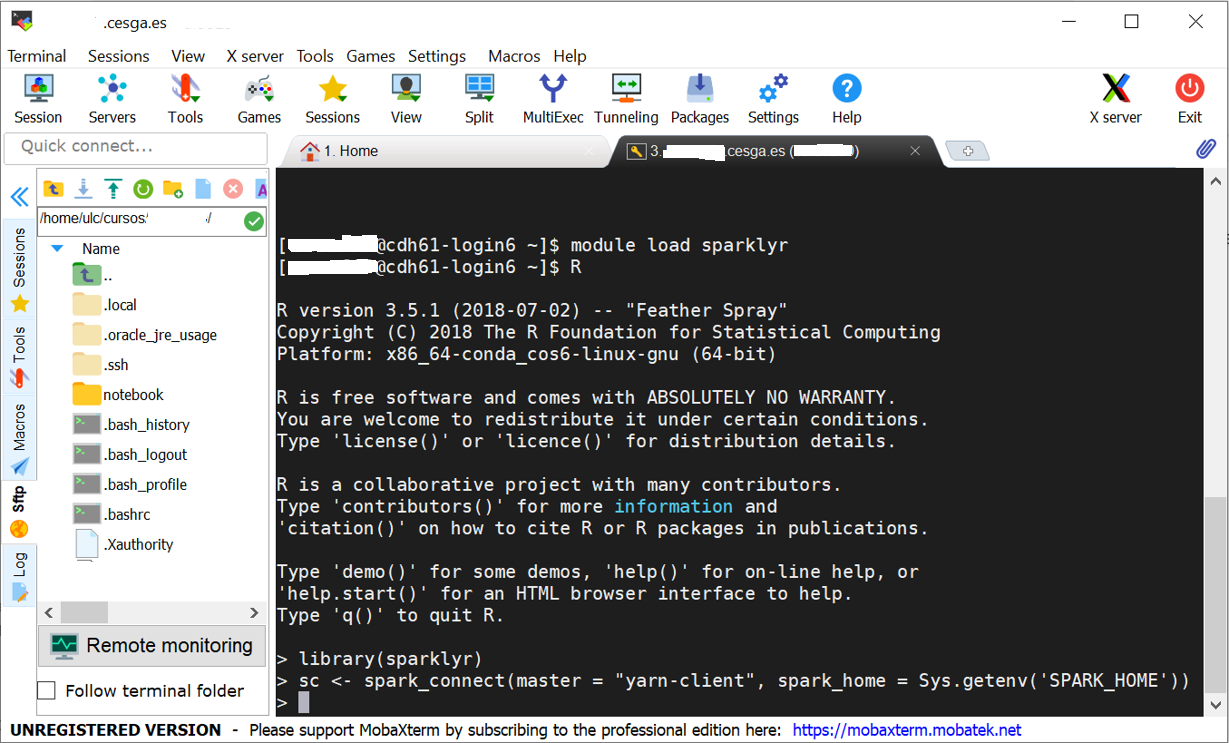
\includegraphics{images/T3-sparklyr1.png}
\caption{}
\end{figure}

O alternativamente mediante jupyterlab. Para ello hacemos los dos
primeros pasos del apartado anterior, conexión vía SSH a CESGA (siempre
con VPN activada!) y una vez dentro ``module load sparklyr''. Y a
continuación escribimos ``start-jupyter-lab'' y nos conectamos a la URL
indicada, desde la cual tendremos acceso a los notebooks Python/R:

\begin{figure}
\centering
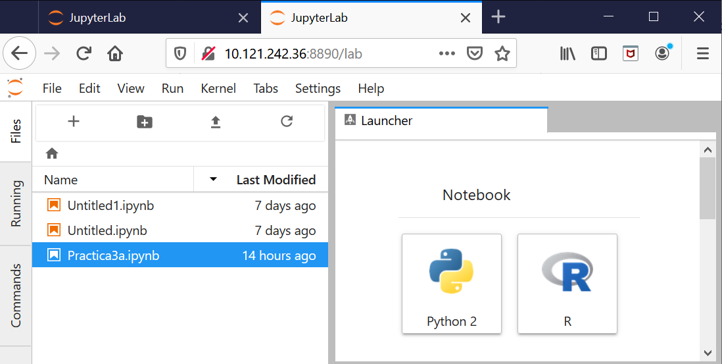
\includegraphics{images/T3-sparklyr2.png}
\caption{}
\end{figure}

Y dentro del notebook R ya se puede probar el funcionamiento de Sparklyr
con los siguientes pasos, cuyo resultado debería ser el que se aprecia a
continuación:

\begin{Shaded}
\begin{Highlighting}[]
\KeywordTok{library}\NormalTok{(sparklyr)}
\NormalTok{sc <-}\StringTok{ }\KeywordTok{spark_connect}\NormalTok{(}\DataTypeTok{master =} \StringTok{"yarn-client"}\NormalTok{, }\DataTypeTok{spark_home =} \KeywordTok{Sys.getenv}\NormalTok{(}\StringTok{'SPARK_HOME'}\NormalTok{)) }
\NormalTok{iris_tbl <-}\StringTok{ }\KeywordTok{copy_to}\NormalTok{(sc, iris, }\StringTok{"iris"}\NormalTok{, }\DataTypeTok{overwrite =} \OtherTok{TRUE}\NormalTok{)}
\NormalTok{iris_tbl}
\end{Highlighting}
\end{Shaded}

\begin{figure}
\centering
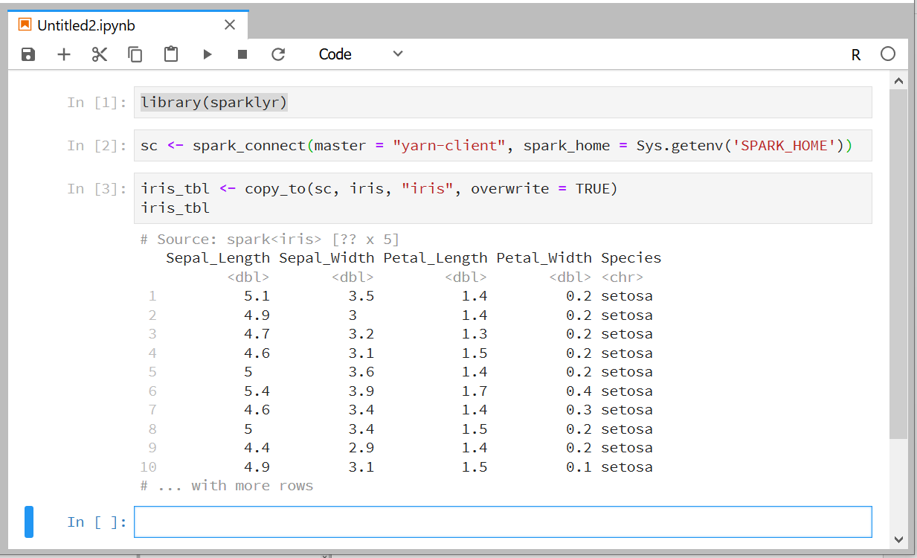
\includegraphics{images/T3-sparklyr3.png}
\caption{}
\end{figure}

NOTA: en ausencia de clúster Hadoop con YARN, o para debugging, también
se puede conectar usando las siguientes instrucciones, y obtener elm
mismo resultado que en presencia de YARN.

\begin{Shaded}
\begin{Highlighting}[]
\KeywordTok{library}\NormalTok{(sparklyr)}
\NormalTok{sc <-}\StringTok{ }\KeywordTok{spark_connect}\NormalTok{(}\DataTypeTok{master =} \StringTok{"local"}\NormalTok{)}
\NormalTok{iris_tbl <-}\StringTok{ }\KeywordTok{copy_to}\NormalTok{(sc, iris, }\StringTok{"iris"}\NormalTok{, }\DataTypeTok{overwrite =} \OtherTok{TRUE}\NormalTok{)}
\NormalTok{iris_tbl}
\end{Highlighting}
\end{Shaded}

\section{Visualización y Generación de Cuadros de
Mando}\label{visualizaciuxf3n-y-generaciuxf3n-de-cuadros-de-mando}

Se sigue un tutorial de la herramienta
\href{https://docs.microsoft.com/es-es/power-bi/desktop-tutorial-analyzing-sales-data-from-excel-and-an-odata-feed}{PowerBI,
con datos de Excel y OData Feed}

Como documentación de se soporte se cuenta con la web de
\href{https://docs.microsoft.com/es-es/power-bi/}{PowerBI} y
\href{https://ccance.net/manuales/powerbi/capitulo_01_introduccion.pdf}{un
tutorial adicional}

\section{Introducción al Análisis de Datos
Masivos}\label{introducciuxf3n-al-anuxe1lisis-de-datos-masivos}

En primer lugar se ha de considerar explorar los datos y realizar
minería con ellos, y eso es posible hacerlo vía Sparklyr, como hemos
visto, o para un análisis más visual, Rattle, que se presenta a
continuación:

\subsection{Rattle}\label{rattle}

Es un paquete para R, con interfaz gráfica desarrollada en GTK, que
permite generar código R para minería de datos. Se instala según los
pasos indicados a continuación:

\begin{Shaded}
\begin{Highlighting}[]
\KeywordTok{install.packages}\NormalTok{(}\StringTok{"ggplot2"}\NormalTok{)}
\KeywordTok{install.packages}\NormalTok{(}\StringTok{"cairoDevice"}\NormalTok{)}
\KeywordTok{install.packages}\NormalTok{(}\StringTok{"RGtk2"}\NormalTok{)}
\KeywordTok{library}\NormalTok{(}\StringTok{"RGtk2"}\NormalTok{)}
\KeywordTok{install.packages}\NormalTok{(}\StringTok{"rattle"}\NormalTok{)}
\KeywordTok{library}\NormalTok{(rattle)}
\KeywordTok{rattle}\NormalTok{()}
\end{Highlighting}
\end{Shaded}

Un tutorial adecuado para introducirse en Rattle es
\href{https://www.dummies.com/programming/using-rattle-iris-r-programming/}{éste}

\begin{figure}
\centering
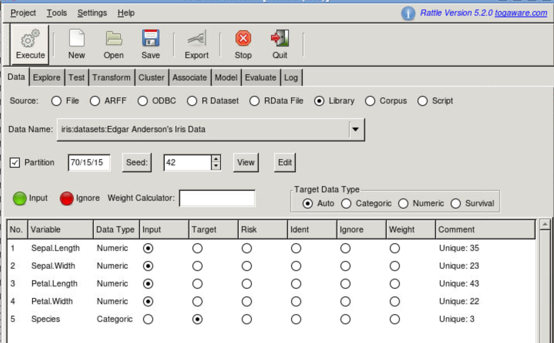
\includegraphics{images/T3-rattle1.png}
\caption{}
\end{figure}

Con el tutorial se pueden ver las capacidades de rattle de explorar los
datos, como se puede apreciar a continuación.

\begin{figure}
\centering
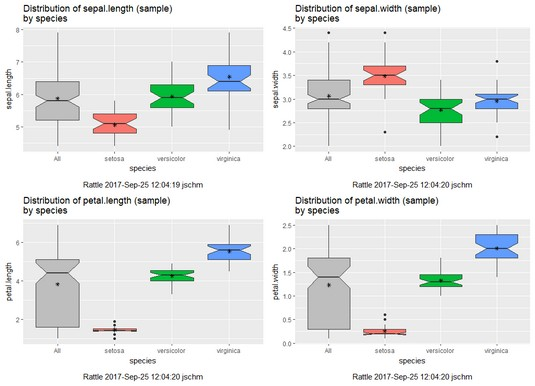
\includegraphics{images/T3-rattle2.png}
\caption{}
\end{figure}

\begin{figure}
\centering
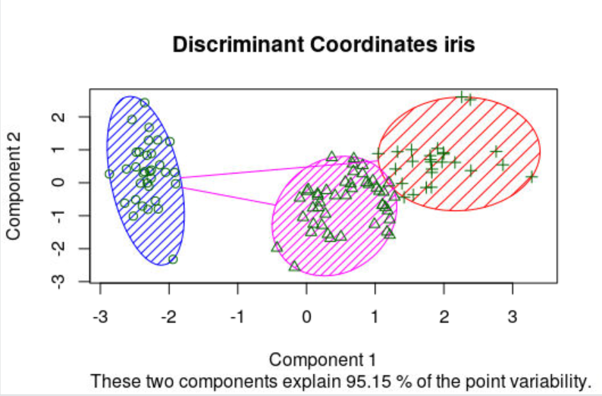
\includegraphics{images/T3-rattle3.png}
\caption{}
\end{figure}

\subsection{Combinando los distintos
elementos}\label{combinando-los-distintos-elementos}

Vamos a seguir
\href{http://hua-zhou.github.io/teaching/biostatm280-2019winter/slides/16-sparklyr/sparklyr-intro.html}{un
tutorial de análisis de datos de vuelos}, adaptándolo al entorno del
CESGA.

En primer lugar, tras conectarnos por ssh al CESGA, y en el mismo
directorio en que hemos hecho la conexión, nos descargamos los datos:

\begin{Shaded}
\begin{Highlighting}[]
\CommentTok{# Make download directory}
\NormalTok{mkdir flights}

\CommentTok{# Download flight data by year}
\ControlFlowTok{for}\NormalTok{ i }\ControlFlowTok{in}\NormalTok{ \{}\DecValTok{1987}\NormalTok{..}\DecValTok{2008}\NormalTok{\}}
\NormalTok{  do}
\NormalTok{    echo }\StringTok{"$(date) $i Download"}
\NormalTok{    fnam=}\ErrorTok{$}\NormalTok{i.csv.bz2}
\NormalTok{    wget }\OperatorTok{-}\NormalTok{O flights}\OperatorTok{/}\ErrorTok{$}\NormalTok{fnam http}\OperatorTok{:}\ErrorTok{//}\NormalTok{stat}\OperatorTok{-}\NormalTok{computing.org}\OperatorTok{/}\NormalTok{dataexpo}\OperatorTok{/}\DecValTok{2009}\OperatorTok{/}\ErrorTok{$}\NormalTok{fnam}
\NormalTok{    echo }\StringTok{"$(date) $i Unzip"}
\NormalTok{    bunzip2 flights}\OperatorTok{/}\ErrorTok{$}\NormalTok{fnam}
\NormalTok{  done}

\CommentTok{# Download airline carrier data}
\NormalTok{wget }\OperatorTok{-}\NormalTok{O airlines.csv http}\OperatorTok{:}\ErrorTok{//}\NormalTok{www.transtats.bts.gov}\OperatorTok{/}\NormalTok{Download_Lookup.asp?Lookup=L_UNIQUE_CARRIERS}

\CommentTok{# Download airports data}
\NormalTok{wget }\OperatorTok{-}\NormalTok{O airports.csv https}\OperatorTok{:}\ErrorTok{//}\NormalTok{raw.githubusercontent.com}\OperatorTok{/}\NormalTok{jpatokal}\OperatorTok{/}\NormalTok{openflights}\OperatorTok{/}\NormalTok{master}\OperatorTok{/}\NormalTok{data}\OperatorTok{/}\NormalTok{airports.dat}
\end{Highlighting}
\end{Shaded}

Comprobamos que los datos están correctos:

\begin{Shaded}
\begin{Highlighting}[]
\NormalTok{head flights}\OperatorTok{/}\FloatTok{1987.}\NormalTok{csv }
\NormalTok{head airlines.csv}
\NormalTok{head airports.csv}
\end{Highlighting}
\end{Shaded}

Y los copiamos al HDFS a través del comando fs de Hadoop:

\begin{Shaded}
\begin{Highlighting}[]
\CommentTok{# Copy flight data to HDFS}
\NormalTok{hadoop fs }\OperatorTok{-}\NormalTok{put flights }

\CommentTok{# Copy airline data to HDFS}
\NormalTok{hadoop fs }\OperatorTok{-}\NormalTok{mkdir airlines}\OperatorTok{/}
\NormalTok{hadoop fs }\OperatorTok{-}\NormalTok{put airlines.csv airlines}

\CommentTok{# Copy airport data to HDFS}
\NormalTok{hadoop fs }\OperatorTok{-}\NormalTok{mkdir airports}\OperatorTok{/}
\NormalTok{hadoop fs }\OperatorTok{-}\NormalTok{put airports.csv airports}
\end{Highlighting}
\end{Shaded}

A continuación lanzamos la ejecución de `hive':

\begin{Shaded}
\begin{Highlighting}[]
\OperatorTok{$}\StringTok{ }\NormalTok{hive}
\end{Highlighting}
\end{Shaded}

Y creamos los metadatos que estructurarán la tabla de vuelos y cargamos
los datos en la tabla Hive:

\begin{Shaded}
\begin{Highlighting}[]
\CommentTok{# Create metadata for flights}
\NormalTok{CREATE EXTERNAL TABLE IF NOT EXISTS flights230}
\NormalTok{(}
\NormalTok{year int,}
\NormalTok{month int,}
\NormalTok{dayofmonth int,}
\NormalTok{dayofweek int,}
\NormalTok{deptime int,}
\NormalTok{crsdeptime int,}
\NormalTok{arrtime int, }
\NormalTok{crsarrtime int,}
\NormalTok{uniquecarrier string,}
\NormalTok{flightnum int,}
\NormalTok{tailnum string, }
\NormalTok{actualelapsedtime int,}
\NormalTok{crselapsedtime int,}
\NormalTok{airtime string,}
\NormalTok{arrdelay int,}
\NormalTok{depdelay int, }
\NormalTok{origin string,}
\NormalTok{dest string,}
\NormalTok{distance int,}
\NormalTok{taxiin string,}
\NormalTok{taxiout string,}
\NormalTok{cancelled int,}
\NormalTok{cancellationcode string,}
\NormalTok{diverted int,}
\NormalTok{carrierdelay string,}
\NormalTok{weatherdelay string,}
\NormalTok{nasdelay string,}
\NormalTok{securitydelay string,}
\NormalTok{lateaircraftdelay string}
\NormalTok{)}
\NormalTok{ROW FORMAT DELIMITED}
\NormalTok{FIELDS TERMINATED BY }\StringTok{','}
\NormalTok{LINES TERMINATED BY }\StringTok{'}\CharTok{\textbackslash{}n}\StringTok{'}
\KeywordTok{TBLPROPERTIES}\NormalTok{(}\StringTok{"skip.header.line.count"}\NormalTok{=}\StringTok{"1"}\NormalTok{);}

\CommentTok{# Load data into table}
\NormalTok{LOAD DATA INPATH }\StringTok{'flights'}\NormalTok{ INTO TABLE flights230;}
\end{Highlighting}
\end{Shaded}

Ídem para la tabla de aerolíneas, creamos los metadatos y cargamos los
datos en la tabla HIVE:

\begin{Shaded}
\begin{Highlighting}[]
\CommentTok{# Create metadata for airlines}
\NormalTok{CREATE EXTERNAL TABLE IF NOT EXISTS airlines}
\NormalTok{(}
\NormalTok{Code string,}
\NormalTok{Description string}
\NormalTok{)}
\NormalTok{ROW FORMAT SERDE }\StringTok{'org.apache.hadoop.hive.serde2.OpenCSVSerde'}
\NormalTok{WITH SERDEPROPERTIES}
\NormalTok{(}
\StringTok{"separatorChar"}\NormalTok{ =}\StringTok{ '\textbackslash{},'}\NormalTok{,}
\StringTok{"quoteChar"}\NormalTok{     =}\StringTok{ '}\CharTok{\textbackslash{}"}\StringTok{'}
\NormalTok{)}
\NormalTok{STORED AS TEXTFILE}
\KeywordTok{tblproperties}\NormalTok{(}\StringTok{"skip.header.line.count"}\NormalTok{=}\StringTok{"1"}\NormalTok{);}

\CommentTok{# Load data into table}
\NormalTok{LOAD DATA INPATH }\StringTok{'airlines'}\NormalTok{ INTO TABLE airlines;}
\end{Highlighting}
\end{Shaded}

Ídem para la tabla de aeropuertos, creamos los metadatos y cargamos los
datos en la tabla HIVE:

\begin{Shaded}
\begin{Highlighting}[]
\CommentTok{# Create metadata for airports}
\NormalTok{CREATE EXTERNAL TABLE IF NOT EXISTS airports}
\NormalTok{(}
\NormalTok{id string,}
\NormalTok{name string,}
\NormalTok{city string,}
\NormalTok{country string,}
\NormalTok{faa string,}
\NormalTok{icao string,}
\NormalTok{lat double,}
\NormalTok{lon double,}
\NormalTok{alt int,}
\NormalTok{tz_offset double,}
\NormalTok{dst string,}
\NormalTok{tz_name string}
\NormalTok{)}
\NormalTok{ROW FORMAT SERDE }\StringTok{'org.apache.hadoop.hive.serde2.OpenCSVSerde'}
\NormalTok{WITH SERDEPROPERTIES}
\NormalTok{(}
\StringTok{"separatorChar"}\NormalTok{ =}\StringTok{ '\textbackslash{},'}\NormalTok{,}
\StringTok{"quoteChar"}\NormalTok{     =}\StringTok{ '}\CharTok{\textbackslash{}"}\StringTok{'}
\NormalTok{)}
\NormalTok{STORED AS TEXTFILE;}

\CommentTok{# Load data into table}
\NormalTok{LOAD DATA INPATH }\StringTok{'airports'}\NormalTok{ INTO TABLE airports;}
\end{Highlighting}
\end{Shaded}

Nos conectamos a Spark (desde jupyter-lab o R): (alternativamente con
`sc \textless{}- spark\_connect(master = ``local'')' )

\begin{Shaded}
\begin{Highlighting}[]
\CommentTok{# Connect to Spark}
\KeywordTok{library}\NormalTok{(sparklyr)}
\KeywordTok{library}\NormalTok{(dplyr)}
\KeywordTok{library}\NormalTok{(ggplot2)}
\NormalTok{sc <-}\StringTok{ }\KeywordTok{spark_connect}\NormalTok{(}\DataTypeTok{master =} \StringTok{"yarn-client"}\NormalTok{, }\DataTypeTok{spark_home =} \KeywordTok{Sys.getenv}\NormalTok{(}\StringTok{'SPARK_HOME'}\NormalTok{)) }
\NormalTok{sc}
\end{Highlighting}
\end{Shaded}

Si tenemos problemas para conectar podemos gestionar con YARN los
recursos

\begin{Shaded}
\begin{Highlighting}[]
\CommentTok{# Ver trabajos en YARN}
\NormalTok{yarn top}

\CommentTok{# Trabajos YARN en ejecución, en espera y aceptados}
\NormalTok{yarn application }\OperatorTok{-}\NormalTok{list }\OperatorTok{|}\StringTok{ }\NormalTok{grep RUNNING}
\NormalTok{yarn application }\OperatorTok{-}\NormalTok{list }\OperatorTok{|}\StringTok{ }\NormalTok{grep ACCEPTED}
\NormalTok{yarn application }\OperatorTok{-}\NormalTok{list }\OperatorTok{|}\StringTok{ }\NormalTok{grep SUBMITTED}

\CommentTok{# Cómo matar un trabajo YARN (si es de nuestro usuario). Indicar el ID de aplicación}
\NormalTok{yarn application }\OperatorTok{-}\NormalTok{kill application_1575999528886_}\DecValTok{0161}
\end{Highlighting}
\end{Shaded}

Crear tablas dplyr a tablas HIVE:

\begin{Shaded}
\begin{Highlighting}[]
\CommentTok{# Cache flights Hive table into Spark}
\CommentTok{#tbl_cache(sc, 'flights')}
\NormalTok{flights_tbl <-}\StringTok{ }\KeywordTok{tbl}\NormalTok{(sc, }\StringTok{'flights230'}\NormalTok{)}
\NormalTok{flights_tbl }\OperatorTok\StringTok{ }\KeywordTok{print}\NormalTok{(}\DataTypeTok{width =} \OtherTok{Inf}\NormalTok{)}
\end{Highlighting}
\end{Shaded}

\begin{Shaded}
\begin{Highlighting}[]
\CommentTok{# Cache airlines Hive table into Spark}
\CommentTok{#tbl_cache(sc, 'airlines')}
\NormalTok{airlines_tbl <-}\StringTok{ }\KeywordTok{tbl}\NormalTok{(sc, }\StringTok{'airlines'}\NormalTok{)}
\NormalTok{airlines_tbl }\OperatorTok\StringTok{ }\KeywordTok{print}\NormalTok{(}\DataTypeTok{width =} \OtherTok{Inf}\NormalTok{)}
\end{Highlighting}
\end{Shaded}

\begin{Shaded}
\begin{Highlighting}[]
\CommentTok{# Cache airports Hive table into Spark}
\CommentTok{#tbl_cache(sc, 'airports')}
\NormalTok{airports_tbl <-}\StringTok{ }\KeywordTok{tbl}\NormalTok{(sc, }\StringTok{'airports'}\NormalTok{)}
\NormalTok{airports_tbl }\OperatorTok\StringTok{ }\KeywordTok{print}\NormalTok{(}\DataTypeTok{width =} \OtherTok{Inf}\NormalTok{)}
\end{Highlighting}
\end{Shaded}

Ejemplos de análisis exploratorio de datos. Todos los vuelos por año:

\begin{Shaded}
\begin{Highlighting}[]
\KeywordTok{system.time}\NormalTok{(\{}
\NormalTok{out <-}\StringTok{ }\NormalTok{flights_tbl }\OperatorTok
\StringTok{  }\KeywordTok{group_by}\NormalTok{(year) }\OperatorTok
\StringTok{  }\KeywordTok{count}\NormalTok{() }\OperatorTok
\StringTok{  }\KeywordTok{arrange}\NormalTok{(year) }\OperatorTok
\StringTok{  }\KeywordTok{collect}\NormalTok{()}
\NormalTok{\})}
\NormalTok{out}
\NormalTok{out }\OperatorTok\StringTok{ }\KeywordTok{ggplot}\NormalTok{(}\KeywordTok{aes}\NormalTok{(}\DataTypeTok{x =}\NormalTok{ year, }\DataTypeTok{y =}\NormalTok{ n)) }\OperatorTok{+}\StringTok{ }\KeywordTok{geom_col}\NormalTok{()}
\end{Highlighting}
\end{Shaded}

Vuelos con origen LAX (Los Angeles) por año:

\begin{Shaded}
\begin{Highlighting}[]
\KeywordTok{system.time}\NormalTok{(\{}
\NormalTok{out <-}\StringTok{ }\NormalTok{flights_tbl }\OperatorTok
\StringTok{  }\KeywordTok{filter}\NormalTok{(origin }\OperatorTok{==}\StringTok{ "LAX"}\NormalTok{) }\OperatorTok
\StringTok{  }\KeywordTok{group_by}\NormalTok{(year) }\OperatorTok
\StringTok{  }\KeywordTok{count}\NormalTok{() }\OperatorTok
\StringTok{  }\KeywordTok{arrange}\NormalTok{(year) }\OperatorTok
\StringTok{  }\KeywordTok{collect}\NormalTok{()}
\NormalTok{\})}
\NormalTok{out}
\NormalTok{out }\OperatorTok\StringTok{ }\KeywordTok{ggplot}\NormalTok{(}\KeywordTok{aes}\NormalTok{(}\DataTypeTok{x =}\NormalTok{ year, }\DataTypeTok{y =}\NormalTok{ n)) }\OperatorTok{+}\StringTok{ }
\StringTok{    }\KeywordTok{geom_col}\NormalTok{() }\OperatorTok{+}
\StringTok{    }\KeywordTok{labs}\NormalTok{(}\DataTypeTok{title =} \StringTok{"Number of flights from LAX"}\NormalTok{)}
\end{Highlighting}
\end{Shaded}

Y listado de países y número de aeropuertos:

\begin{Shaded}
\begin{Highlighting}[]
\KeywordTok{system.time}\NormalTok{(\{}
\NormalTok{out <-}\StringTok{ }\NormalTok{airports_tbl }\OperatorTok
\StringTok{  }\KeywordTok{group_by}\NormalTok{(}\StringTok{"country"}\NormalTok{) }\OperatorTok
\StringTok{  }\KeywordTok{count}\NormalTok{()}
\NormalTok{\})}
\NormalTok{out}
\end{Highlighting}
\end{Shaded}

Vamos a proceder a generar un conjunto de datos para calcular un modelo.
Para ello buscaremos modelar como una regresión lineal la ganancia de un
vuelo (gain) como (depdelay - arrdelay) basándose en la distancia, el
retraso de la salida y la aerolínea usando datos del período 2003-2007:

\begin{Shaded}
\begin{Highlighting}[]
\CommentTok{# Filter records and create target variable 'gain'}
\KeywordTok{system.time}\NormalTok{(}
\NormalTok{  model_data <-}\StringTok{ }\NormalTok{flights_tbl }\OperatorTok
\StringTok{    }\KeywordTok{filter}\NormalTok{(}\OperatorTok{!}\KeywordTok{is.na}\NormalTok{(arrdelay) }\OperatorTok{&}\StringTok{ }\OperatorTok{!}\KeywordTok{is.na}\NormalTok{(depdelay) }\OperatorTok{&}\StringTok{ }\OperatorTok{!}\KeywordTok{is.na}\NormalTok{(distance)) }\OperatorTok
\StringTok{    }\KeywordTok{filter}\NormalTok{(depdelay }\OperatorTok{>}\StringTok{ }\DecValTok{15} \OperatorTok{&}\StringTok{ }\NormalTok{depdelay }\OperatorTok{<}\StringTok{ }\DecValTok{240}\NormalTok{) }\OperatorTok
\StringTok{    }\KeywordTok{filter}\NormalTok{(arrdelay }\OperatorTok{>}\StringTok{ }\OperatorTok{-}\DecValTok{60} \OperatorTok{&}\StringTok{ }\NormalTok{arrdelay }\OperatorTok{<}\StringTok{ }\DecValTok{360}\NormalTok{) }\OperatorTok
\StringTok{    }\KeywordTok{filter}\NormalTok{(year }\OperatorTok{>=}\StringTok{ }\DecValTok{2003} \OperatorTok{&}\StringTok{ }\NormalTok{year }\OperatorTok{<=}\StringTok{ }\DecValTok{2007}\NormalTok{) }\OperatorTok
\StringTok{    }\KeywordTok{left_join}\NormalTok{(airlines_tbl, }\DataTypeTok{by =} \KeywordTok{c}\NormalTok{(}\StringTok{"uniquecarrier"}\NormalTok{ =}\StringTok{ "code"}\NormalTok{)) }\OperatorTok
\StringTok{    }\KeywordTok{mutate}\NormalTok{(}\DataTypeTok{gain =}\NormalTok{ depdelay }\OperatorTok{-}\StringTok{ }\NormalTok{arrdelay) }\OperatorTok
\StringTok{    }\KeywordTok{select}\NormalTok{(year, month, arrdelay, depdelay, distance, uniquecarrier, description, gain)}
\NormalTok{)}
\NormalTok{model_data}
\end{Highlighting}
\end{Shaded}

\begin{Shaded}
\begin{Highlighting}[]
\CommentTok{# Summarize data by carrier}
\NormalTok{model_data }\OperatorTok
\StringTok{  }\KeywordTok{group_by}\NormalTok{(uniquecarrier) }\OperatorTok
\StringTok{  }\KeywordTok{summarize}\NormalTok{(}\DataTypeTok{description =} \KeywordTok{min}\NormalTok{(description), }\DataTypeTok{gain =} \KeywordTok{mean}\NormalTok{(gain), }
            \DataTypeTok{distance =} \KeywordTok{mean}\NormalTok{(distance), }\DataTypeTok{depdelay =} \KeywordTok{mean}\NormalTok{(depdelay)) }\OperatorTok
\StringTok{  }\KeywordTok{select}\NormalTok{(description, gain, distance, depdelay) }\OperatorTok
\StringTok{  }\KeywordTok{arrange}\NormalTok{(gain)}
\end{Highlighting}
\end{Shaded}

Para entrenar la regresión lineal y predecir el tiempo ganado o perdido
en un vuelo en función de la distancia, retraso en la salida y aerolínea
procedemos de este modo:

\begin{Shaded}
\begin{Highlighting}[]
\CommentTok{# Partition the data into training and validation sets}
\NormalTok{model_partition <-}\StringTok{ }\NormalTok{model_data }\OperatorTok\StringTok{ }
\StringTok{  }\KeywordTok{sdf_partition}\NormalTok{(}\DataTypeTok{train =} \FloatTok{0.8}\NormalTok{, }\DataTypeTok{valid =} \FloatTok{0.2}\NormalTok{, }\DataTypeTok{seed =} \DecValTok{5555}\NormalTok{)}

\CommentTok{# Fit a linear model}
\KeywordTok{system.time}\NormalTok{(}
\NormalTok{  ml1 <-}\StringTok{ }\NormalTok{model_partition}\OperatorTok{$}\NormalTok{train }\OperatorTok
\StringTok{    }\KeywordTok{ml_linear_regression}\NormalTok{(gain }\OperatorTok{~}\StringTok{ }\NormalTok{distance }\OperatorTok{+}\StringTok{ }\NormalTok{depdelay }\OperatorTok{+}\StringTok{ }\NormalTok{uniquecarrier)}
\NormalTok{)}

\CommentTok{# Summarize the linear model}
\KeywordTok{summary}\NormalTok{(ml1)}
\end{Highlighting}
\end{Shaded}

A continuación se compara la bondad del modelo con el subconjunto de
validación

\begin{Shaded}
\begin{Highlighting}[]
\CommentTok{# Calculate average gains by predicted decile}
\KeywordTok{system.time}\NormalTok{(}
\NormalTok{  model_deciles <-}\StringTok{ }\KeywordTok{lapply}\NormalTok{(model_partition, }\ControlFlowTok{function}\NormalTok{(x) \{}
    \KeywordTok{ml_predict}\NormalTok{(ml1, x) }\OperatorTok
\StringTok{      }\KeywordTok{mutate}\NormalTok{(}\DataTypeTok{decile =} \KeywordTok{ntile}\NormalTok{(}\KeywordTok{desc}\NormalTok{(prediction), }\DecValTok{10}\NormalTok{)) }\OperatorTok
\StringTok{      }\KeywordTok{group_by}\NormalTok{(decile) }\OperatorTok
\StringTok{      }\KeywordTok{summarize}\NormalTok{(}\DataTypeTok{gain =} \KeywordTok{mean}\NormalTok{(gain)) }\OperatorTok
\StringTok{      }\KeywordTok{select}\NormalTok{(decile, gain) }\OperatorTok
\StringTok{      }\KeywordTok{collect}\NormalTok{()}
\NormalTok{  \})}
\NormalTok{)}
\NormalTok{model_deciles}

\CommentTok{# Create a summary dataset for plotting}
\NormalTok{deciles <-}\StringTok{ }\KeywordTok{rbind}\NormalTok{(}
  \KeywordTok{data.frame}\NormalTok{(}\DataTypeTok{data =} \StringTok{'train'}\NormalTok{, model_deciles}\OperatorTok{$}\NormalTok{train),}
  \KeywordTok{data.frame}\NormalTok{(}\DataTypeTok{data =} \StringTok{'valid'}\NormalTok{, model_deciles}\OperatorTok{$}\NormalTok{valid),}
  \DataTypeTok{make.row.names =} \OtherTok{FALSE}
\NormalTok{)}
\NormalTok{deciles}

\CommentTok{# Plot average gains by predicted decile}
\NormalTok{deciles }\OperatorTok
\StringTok{  }\KeywordTok{ggplot}\NormalTok{(}\KeywordTok{aes}\NormalTok{(}\KeywordTok{factor}\NormalTok{(decile), gain, }\DataTypeTok{fill =}\NormalTok{ data)) }\OperatorTok{+}
\StringTok{  }\KeywordTok{geom_bar}\NormalTok{(}\DataTypeTok{stat =} \StringTok{'identity'}\NormalTok{, }\DataTypeTok{position =} \StringTok{'dodge'}\NormalTok{) }\OperatorTok{+}
\StringTok{  }\KeywordTok{labs}\NormalTok{(}\DataTypeTok{title =} \StringTok{'Average gain by predicted decile'}\NormalTok{, }\DataTypeTok{x =} \StringTok{'Decile'}\NormalTok{, }\DataTypeTok{y =} \StringTok{'Minutes'}\NormalTok{)}
\end{Highlighting}
\end{Shaded}

Visualizar predicciones usando el año 2008 (no usado en el
entrenamiento):

\begin{Shaded}
\begin{Highlighting}[]
\CommentTok{# Select data from an out of time sample}
\NormalTok{data_}\DecValTok{2008}\NormalTok{ <-}\StringTok{ }\NormalTok{flights_tbl }\OperatorTok
\StringTok{  }\KeywordTok{filter}\NormalTok{(}\OperatorTok{!}\KeywordTok{is.na}\NormalTok{(arrdelay) }\OperatorTok{&}\StringTok{ }\OperatorTok{!}\KeywordTok{is.na}\NormalTok{(depdelay) }\OperatorTok{&}\StringTok{ }\OperatorTok{!}\KeywordTok{is.na}\NormalTok{(distance)) }\OperatorTok
\StringTok{  }\KeywordTok{filter}\NormalTok{(depdelay }\OperatorTok{>}\StringTok{ }\DecValTok{15} \OperatorTok{&}\StringTok{ }\NormalTok{depdelay }\OperatorTok{<}\StringTok{ }\DecValTok{240}\NormalTok{) }\OperatorTok
\StringTok{  }\KeywordTok{filter}\NormalTok{(arrdelay }\OperatorTok{>}\StringTok{ }\OperatorTok{-}\DecValTok{60} \OperatorTok{&}\StringTok{ }\NormalTok{arrdelay }\OperatorTok{<}\StringTok{ }\DecValTok{360}\NormalTok{) }\OperatorTok
\StringTok{  }\KeywordTok{filter}\NormalTok{(year }\OperatorTok{==}\StringTok{ }\DecValTok{2008}\NormalTok{) }\OperatorTok
\StringTok{  }\KeywordTok{left_join}\NormalTok{(airlines_tbl, }\DataTypeTok{by =} \KeywordTok{c}\NormalTok{(}\StringTok{"uniquecarrier"}\NormalTok{ =}\StringTok{ "code"}\NormalTok{)) }\OperatorTok
\StringTok{  }\KeywordTok{mutate}\NormalTok{(}\DataTypeTok{gain =}\NormalTok{ depdelay }\OperatorTok{-}\StringTok{ }\NormalTok{arrdelay) }\OperatorTok
\StringTok{  }\KeywordTok{select}\NormalTok{(year, month, arrdelay, depdelay, distance, uniquecarrier, description, gain, origin, dest)}
\NormalTok{data_}\DecValTok{2008}

\CommentTok{# Summarize data by carrier}
\NormalTok{carrier <-}\StringTok{ }\KeywordTok{ml_predict}\NormalTok{(ml1, data_}\DecValTok{2008}\NormalTok{) }\OperatorTok
\StringTok{  }\KeywordTok{group_by}\NormalTok{(description) }\OperatorTok
\StringTok{  }\KeywordTok{summarize}\NormalTok{(}\DataTypeTok{gain =} \KeywordTok{mean}\NormalTok{(gain), }\DataTypeTok{prediction =} \KeywordTok{mean}\NormalTok{(prediction), }\DataTypeTok{freq =} \KeywordTok{n}\NormalTok{()) }\OperatorTok
\StringTok{  }\KeywordTok{filter}\NormalTok{(freq }\OperatorTok{>}\StringTok{ }\DecValTok{10000}\NormalTok{) }\OperatorTok
\StringTok{  }\KeywordTok{collect}\NormalTok{()}
\NormalTok{carrier}

\CommentTok{# Plot actual gains and predicted gains by airline carrier}
\KeywordTok{ggplot}\NormalTok{(carrier, }\KeywordTok{aes}\NormalTok{(gain, prediction)) }\OperatorTok{+}\StringTok{ }
\StringTok{  }\KeywordTok{geom_point}\NormalTok{(}\DataTypeTok{alpha =} \FloatTok{0.75}\NormalTok{, }\DataTypeTok{color =} \StringTok{'red'}\NormalTok{, }\DataTypeTok{shape =} \DecValTok{3}\NormalTok{) }\OperatorTok{+}
\StringTok{  }\KeywordTok{geom_abline}\NormalTok{(}\DataTypeTok{intercept =} \DecValTok{0}\NormalTok{, }\DataTypeTok{slope =} \DecValTok{1}\NormalTok{, }\DataTypeTok{alpha =} \FloatTok{0.15}\NormalTok{, }\DataTypeTok{color =} \StringTok{'blue'}\NormalTok{) }\OperatorTok{+}
\StringTok{  }\KeywordTok{geom_text}\NormalTok{(}\KeywordTok{aes}\NormalTok{(}\DataTypeTok{label =} \KeywordTok{substr}\NormalTok{(description, }\DecValTok{1}\NormalTok{, }\DecValTok{20}\NormalTok{)), }\DataTypeTok{size =} \DecValTok{3}\NormalTok{, }\DataTypeTok{alpha =} \FloatTok{0.75}\NormalTok{, }\DataTypeTok{vjust =} \OperatorTok{-}\DecValTok{1}\NormalTok{) }\OperatorTok{+}
\StringTok{  }\KeywordTok{labs}\NormalTok{(}\DataTypeTok{title=}\StringTok{'Average Gains Forecast'}\NormalTok{, }\DataTypeTok{x =} \StringTok{'Actual'}\NormalTok{, }\DataTypeTok{y =} \StringTok{'Predicted'}\NormalTok{)}
\end{Highlighting}
\end{Shaded}

Al terminar cualquier ejercicio con sparklyr desconectamos de Spark:

\begin{Shaded}
\begin{Highlighting}[]
\KeywordTok{spark_disconnect_all}\NormalTok{()}
\end{Highlighting}
\end{Shaded}

\section{Práctica 3: Big Data}\label{pruxe1ctica-3-big-data}

Los ejercicios se entregarán por correo electrónico a
\href{mailto:guillermo.lopez.taboada@udc.es}{\nolinkurl{guillermo.lopez.taboada@udc.es}}
en formato PDF o R MarkDown con el nombre de archivo
P3X-Apellidos-Nombre.Rmd (sin tildes ni caracteres especiales en el
nombre del arhivo) \textbf{antes} del miércoles 18 de Diciembre.

\subsection{Ejercicio A con sparklyr}\label{ejercicio-a-con-sparklyr}

(3 puntos) Replicación del siguiente ejercicio con sparklyr y el dataset
iris (\url{https://spark.rstudio.com/mlib/}) en modo local o modo YARN.
Puede ser dentro de jupyterlab (así me entregáis archivo
``Apellidos-Nombre.ipynb'') o en R remoto o en Rstudio (vía Desktop de
visualización) (en estos dos últimos casos entregáis
P3A-Apellidos-Nombre.R).

\subsection{Ejercicio B con rattle}\label{ejercicio-b-con-rattle}

(4 puntos) Informe (en PDF) sobre uno de los 4 datasets (audit, weather,
weatherAUS, wine) que se describen a continuación
\url{https://cran.r-project.org/web/packages/rattle.data/rattle.data.pdf}
Se busca que realicéis un análisis con Rattle, mínimo con las pestañas
Explore, Cluster y Model.

\subsection{Ejercicio C con sparklyr y
Hadoop}\label{ejercicio-c-con-sparklyr-y-hadoop}

(3 puntos) Replicación del siguiente ejercicio con sparklyr en el CESGA,
en análisis de los datos del dataset de vuelos:
\url{http://hua-zhou.github.io/teaching/biostatm280-2019winter/slides/16-sparklyr/sparklyr-flights.html}\\
se valorarán análisis adicionales y detalles sobre tiempos de ejecución
de los análisis, espera en colas yarn, listado de trabajos spark,
etc\ldots{}

\appendix


Working draft\ldots{}

\chapter{Enlaces}\label{links}

\textbf{Recursos para el aprendizaje de R} (
\url{https://rubenfcasal.github.io/post/ayuda-y-recursos-para-el-aprendizaje-de-r}
): A continuación se muestran algunos recursos que pueden ser útiles
para el aprendizaje de R y la obtención de ayuda\ldots{}

\textbf{\emph{Ayuda online}}:

\begin{itemize}
\item
  Ayuda en línea sobre funciones o paquetes:
  \href{https://www.rdocumentation.org/}{RDocumentation}
\item
  Buscador \href{http://rseek.org/}{RSeek}
\item
  \href{http://stackoverflow.com/questions/tagged/r}{StackOverflow}
\end{itemize}

\textbf{\emph{Cursos}}: algunos cursos gratuitos:

\begin{itemize}
\item
  \href{https://www.coursera.org/}{Coursera}:

  \begin{itemize}
  \item
    \href{https://www.coursera.org/learn/intro-data-science-programacion-estadistica-r}{Introducción
    a Data Science: Programación Estadística con R}
  \item
    \href{https://www.coursera.org/specializations/r}{Mastering Software
    Development in R}
  \end{itemize}
\end{itemize}

\begin{itemize}
\item
  \href{https://www.datacamp.com/courses}{DataCamp}:

  \begin{itemize}
  \tightlist
  \item
    \href{https://www.datacamp.com/courses/introduccion-a-r/}{Introducción
    a R}
  \end{itemize}
\end{itemize}

\begin{itemize}
\item
  \href{http://online.stanford.edu/courses}{Stanford online}:

  \begin{itemize}
  \tightlist
  \item
    \href{http://online.stanford.edu/course/statistical-learning}{Statistical
    Learning}
  \end{itemize}
\end{itemize}

\begin{itemize}
\tightlist
\item
  Curso UCA:
  \href{http://knuth.uca.es/moodle/course/view.php?id=51}{Introducción a
  R, R-commander y shiny}
\end{itemize}

\begin{itemize}
\tightlist
\item
  Curso \href{https://r-coder.com/curso-r}{R CODER}
\end{itemize}

\begin{itemize}
\tightlist
\item
  Udacity:
  \href{https://eu.udacity.com/course/data-analysis-with-r--ud651}{Data
  Analysis with R}
\end{itemize}

\begin{itemize}
\tightlist
\item
  \href{https://swirlstats.com/scn/title.html}{Swirl Courses}: se pueden
  hacer cursos desde el propio R con el paquete
  \href{https://swirlstats.com}{swirl}.
\end{itemize}

Para información sobre cursos en castellano se puede recurrir a la web
de \href{http://r-es.org/}{R-Hispano} en el apartado
\href{http://r-es.org/category/formacion}{formación}. Algunos de los
cursos que aparecen en entradas antiguas son gratuitos. Ver:
\href{http://r-es.org/2016/02/12/cursos-masivos-y-otra-formacion-on-line-sobre-r/}{Cursos
MOOC relacionados con R}.

\textbf{\emph{Libros}}

\begin{itemize}
\item
  \textbf{\emph{Iniciación}}:

  \begin{itemize}
  \item
    R for Data Science (\href{http://r4ds.had.co.nz/}{online},
    \href{http://shop.oreilly.com/product/0636920034407.do}{O'Reilly})
  \item
    2011 - The Art of R Programming. A Tour of Statistical Software
    Design, (\href{https://www.nostarch.com/artofr.htm}{No Starch
    Press})
  \item
    Hands-On Programming with R: Write Your Own Functions and
    Simulations, by Garrett Grolemund
    (\href{http://shop.oreilly.com/product/0636920028574.do}{O'Reilly})
  \end{itemize}
\item
  \textbf{\emph{Avanzados}}:

  \begin{itemize}
  \item
    Advanced R by Hadley Wickham (online:
    \href{http://adv-r.had.co.nz/}{1ª ed},
    \href{https://adv-r.hadley.nz/}{2ª ed},
    \href{https://www.amazon.com/dp/1466586966}{Chapman \& Hall})
  \item
    2008 - Software for Data Analysis: Programming with R - Chambers
    (\href{http://www.springer.com/la/book/9780387759357}{Springer})
  \item
    R packages by Hadley Wickham
    (\href{http://r-pkgs.had.co.nz/}{online},
    \href{http://shop.oreilly.com/product/0636920034421.do}{O'Reilly})
  \end{itemize}
\item
  \textbf{\emph{Bookdown}}: el paquete
  \href{https://bookdown.org}{\texttt{bookdown}} de R permite escribir
  libros empleando \href{http://rmarkdown.rstudio.com}{R Markdown} y
  compartirlos. En \url{https://bookdown.org} está disponible una
  selección de libros escritos con este paquete (un listado más completo
  está disponible \href{https://bookdown.org/home/archive/}{aquí}).
  Algunos libros en este formato en castellano son:

  \begin{itemize}
  \item
    \href{https://rubenfcasal.github.io/intror}{Introducción al Análisis
    de Datos con R} (disponible en el repositorio de GitHub
    \href{https://github.com/rubenfcasal/intror}{rubenfcasal/intror}).
  \item
    \href{https://rubenfcasal.github.io/simbook}{Prácticas de
    Simulación} (disponible en el repositorio de GitHub
    \href{https://github.com/rubenfcasal/simbook}{rubenfcasal/simbook}).
  \item
    \href{https://rubenfcasal.github.io/bookdown_intro/}{Escritura de
    libros con bookdown} (disponible en el repositorio de GitHub
    \href{https://github.com/rubenfcasal/bookdown_intro}{rubenfcasal/bookdown\_intro}).
  \item
    \href{https://www.datanalytics.com/libro_r/index.html}{R para
    profesionales de los datos: una introducción}.
  \item
    \href{https://bookdown.org/aquintela/EBE}{Estadística Básica
    Edulcorada}.
  \end{itemize}
\end{itemize}

\textbf{\emph{Material online}}: en la web se puede encontrar mucho
material adicional, por ejemplo:

\begin{itemize}
\item
  \href{https://www.r-project.org/other-docs.html}{CRAN: Other R
  documentation}
\item
  Blogs en inglés:

  \begin{itemize}
  \item
    \url{https://www.r-bloggers.com/}
  \item
    \url{https://www.littlemissdata.com/blog/rstudioconf2019}
  \item
    RStudio: \url{https://blog.rstudio.com}
  \item
    Microsoft Revolutions: \url{https://blog.revolutionanalytics.com}
  \end{itemize}
\item
  Blogs en castellano:

  \begin{itemize}
  \item
    \url{https://www.datanalytics.com}
  \item
    \url{http://oscarperpinan.github.io/R}
  \item
    \url{http://rubenfcasal.github.io}
  \end{itemize}
\item
  Listas de correo:

  \begin{itemize}
  \item
    Listas de distribución de r-project.org:
    \url{https://stat.ethz.ch/mailman/listinfo}
  \item
    Búsqueda en R-help:
    \url{http://r.789695.n4.nabble.com/R-help-f789696.html}
  \item
    Búsqueda en R-help-es: \url{https://r-help-es.r-project.narkive.com}

    \url{https://grokbase.com/g/r/r-help-es}
  \item
    Archivos de R-help-es:
    \url{https://stat.ethz.ch/pipermail/r-help-es}
  \end{itemize}
\end{itemize}

\section{RStudio}\label{rstudio-links}

\href{https://www.rstudio.com}{\textbf{\emph{RStudio}}}:

\begin{itemize}
\item
  \href{https://www.rstudio.com/online-learning}{Online learning}
\item
  \href{https://resources.rstudio.com/webinars}{Webinars}
\item
  \href{https://spark.rstudio.com/}{sparklyr}
\item
  \href{http://shiny.rstudio.com}{shiny}
\end{itemize}

\href{https://www.tidyverse.org/}{\textbf{\emph{tidyverse}}}:

\begin{itemize}
\item
  \href{https://dplyr.tidyverse.org}{dplyr}
\item
  \href{https://tibble.tidyverse.org}{tibble}
\item
  \href{https://tidyr.tidyverse.org}{tidyr}
\item
  \href{https://stringr.tidyverse.org}{stringr}
\item
  \href{https://readr.tidyverse.org}{readr}
\item
  \href{https://db.rstudio.com}{Databases using R},
  \href{https://db.rstudio.com/overview}{dplyr as a database interface},
  \href{https://db.rstudio.com/dplyr}{Databases using dplyr}
\end{itemize}

\href{https://resources.rstudio.com/rstudio-cheatsheets}{\textbf{\emph{CheatSheets}}}:

\begin{itemize}
\item
  \href{https://resources.rstudio.com/rstudio-cheatsheets/rmarkdown-2-0-cheat-sheet}{rmarkdown}
\item
  \href{https://resources.rstudio.com/rstudio-cheatsheets/shiny-cheat-sheet}{shiny}
\item
  \href{https://github.com/rstudio/cheatsheets/blob/master/data-transformation.pdf}{dplyr}
\item
  \href{https://github.com/rstudio/cheatsheets/blob/master/data-import.pdf}{tidyr}
\item
  \href{https://resources.rstudio.com/rstudio-cheatsheets/stringr-cheat-sheet}{stringr}
\end{itemize}

\section{Bibliometría}\label{bibliom-links}

\begin{itemize}
\item
  \href{https://cran.r-project.org/web/packages/CITAN/index.html}{CITAN}
\item
  \href{https://rubenfcasal.github.io/scimetr/index.html}{scimetr}
\item
  \href{http://www.bibliometrix.org}{bibliometrix}
\item
  \href{https://vt-arc.github.io/wosr/index.html}{wosr}
\item
  \href{https://github.com/juba/rwos}{rwos}
\item
  \href{https://docs.ropensci.org/rcrossref}{rcrossref}
\item
  \href{https://ropensci.org/packages/}{ropensci}: Literature
\item
  \href{https://cran.r-project.org/web/packages/Diderot/index.html}{Diderot}
\item
  \ldots{}
\end{itemize}

\chapter{El paquete scimetr}\label{scimetr}

Package \texttt{scimetr} implements tools for quantitative research in
scientometrics and bibliometrics. It provides routines for importing
bibliographic data from Thomson Reuters' Web of Science
(\url{http://www.webofknowledge.com}) and performing bibliometric
analysis. For more information visit
\url{https://rubenfcasal.github.io/scimetr/articles/scimetr.html}.

\section{Instalación}\label{instalaciuxf3n}

Para instalar el paquete sería recomendable en primer lugar instalar las
dependencias:

\begin{Shaded}
\begin{Highlighting}[]
\KeywordTok{install.packages}\NormalTok{(}\KeywordTok{c}\NormalTok{(}\StringTok{'dplyr'}\NormalTok{, }\StringTok{'lazyeval'}\NormalTok{, }\StringTok{'stringr'}\NormalTok{, }\StringTok{'ggplot2'}\NormalTok{, }\StringTok{'openxlsx'}\NormalTok{, }\StringTok{'tidyr'}\NormalTok{))}
\end{Highlighting}
\end{Shaded}

Como de momento no está disponible en CRAN, habría que instalar la
versión de desarrollo en GitHub. En Windows bastaría con instalar la
versión binaria del paquete \emph{scimetr\_X.Y.Z.zip} (disponible
\href{https://github.com/rubenfcasal/scimetr/tree/master/docs}{aqui}),
alternativamente se puede instalar directamente de GitHub:

\begin{Shaded}
\begin{Highlighting}[]
\CommentTok{# install.packages("devtools")}
\NormalTok{devtools}\OperatorTok{::}\KeywordTok{install_github}\NormalTok{(}\StringTok{"rubenfcasal/scimetr"}\NormalTok{)}
\end{Highlighting}
\end{Shaded}

Una vez instalado ya podríamos cargar el paquete:

\begin{Shaded}
\begin{Highlighting}[]
\KeywordTok{library}\NormalTok{(scimetr)}
\end{Highlighting}
\end{Shaded}

\section{Carga de datos}\label{carga-de-datos}

\subsection{Datos de ejemplo}\label{datos-de-ejemplo-1}

En el paquete se incluyen dos conjuntos de datos de ejemplo
correspondientes a la búsqueda en WoS por el campo Organización-Nombre
preferido de la UDC (Organization-Enhaced: OG = Universidade da Coruna):

\begin{itemize}
\item
  \texttt{wosdf}: año 2015.
\item
  \texttt{wosdf2}: área de investigación `Mathematics', años 2008-2017.
\end{itemize}

Variables WoS:

\begin{Shaded}
\begin{Highlighting}[]
\CommentTok{# View(wosdf2) # En RStudio...}
\NormalTok{variable.labels <-}\StringTok{ }\KeywordTok{attr}\NormalTok{(wosdf, }\StringTok{"variable.labels"}\NormalTok{)}
\NormalTok{knitr}\OperatorTok{::}\KeywordTok{kable}\NormalTok{(}\KeywordTok{as.data.frame}\NormalTok{(variable.labels)) }\CommentTok{# caption = "Variable labels"}
\end{Highlighting}
\end{Shaded}

\begin{tabular}{l|l}
\hline
  & variable.labels\\
\hline
PT & Publication type\\
\hline
AU & Author\\
\hline
BA & Book authors\\
\hline
BE & Editor\\
\hline
GP & Group author\\
\hline
AF & Author full\\
\hline
BF & Book authors fullname\\
\hline
CA & Corporate author\\
\hline
TI & Title\\
\hline
SO & Publication name\\
\hline
SE & Series title\\
\hline
BS & Book series\\
\hline
LA & Language\\
\hline
DT & Document type\\
\hline
CT & Conference title\\
\hline
CY & Conference year\\
\hline
CL & Conference place\\
\hline
SP & Conference sponsors\\
\hline
HO & Conference host\\
\hline
DE & Keywords\\
\hline
ID & Keywords Plus\\
\hline
AB & Abstract\\
\hline
C1 & Addresses\\
\hline
RP & Reprint author\\
\hline
EM & Author email\\
\hline
RI & Researcher id numbers\\
\hline
OI & Orcid numbers\\
\hline
FU & Funding agency and grant number\\
\hline
FX & Funding text\\
\hline
CR & Cited references\\
\hline
NR & Number of cited references\\
\hline
TC & Times cited\\
\hline
Z9 & Total times cited count\\
\hline
U1 & Usage Count (Last 180 Days)\\
\hline
U2 & Usage Count (Since 2013)\\
\hline
PU & Publisher\\
\hline
PI & Publisher city\\
\hline
PA & Publisher address\\
\hline
SN & ISSN\\
\hline
EI & eISSN\\
\hline
BN & ISBN\\
\hline
J9 & Journal.ISI\\
\hline
JI & Journal.ISO\\
\hline
PD & Publication date\\
\hline
PY & Year published\\
\hline
VL & Volume\\
\hline
IS & Issue\\
\hline
PN & Part number\\
\hline
SU & Supplement\\
\hline
SI & Special issue\\
\hline
MA & Meeting abstract\\
\hline
BP & Beginning page\\
\hline
EP & Ending page\\
\hline
AR & Article number\\
\hline
DI & DOI\\
\hline
D2 & Book DOI\\
\hline
PG & Page count\\
\hline
WC & WOS category\\
\hline
SC & Research areas\\
\hline
GA & Document delivery number\\
\hline
UT & Access number\\
\hline
PM & Pub Med ID\\
\hline
\end{tabular}

Se puede crear una base de datos con la función \texttt{CreateDB.wos()}:

\begin{Shaded}
\begin{Highlighting}[]
\NormalTok{db <-}\StringTok{ }\KeywordTok{CreateDB.wos}\NormalTok{(wosdf2, }\DataTypeTok{label =} \StringTok{"Mathematics_UDC_2008-2017 (01-02-2019)"}\NormalTok{)}
\KeywordTok{str}\NormalTok{(db, }\DecValTok{1}\NormalTok{)}
\end{Highlighting}
\end{Shaded}

\begin{verbatim}
## List of 11
##  $ Docs      :'data.frame':  389 obs. of  26 variables:
##  $ Authors   :'data.frame':  611 obs. of  4 variables:
##  $ AutDoc    :'data.frame':  1260 obs. of  2 variables:
##  $ Categories:'data.frame':  46 obs. of  2 variables:
##  $ CatDoc    :'data.frame':  866 obs. of  2 variables:
##  $ Areas     :'data.frame':  26 obs. of  2 variables:
##  $ AreaDoc   :'data.frame':  771 obs. of  2 variables:
##  $ Addresses :'data.frame':  896 obs. of  5 variables:
##  $ AddAutDoc :'data.frame':  1328 obs. of  3 variables:
##  $ Journals  :'data.frame':  150 obs. of  12 variables:
##  $ label     : chr "Mathematics_UDC_2008-2017 (01-02-2019)"
##  - attr(*, "variable.labels")= Named chr [1:62] "Publication type" "Author" "Book authors" "Editor" ...
##   ..- attr(*, "names")= chr [1:62] "PT" "AU" "BA" "BE" ...
##  - attr(*, "class")= chr "wos.db"
\end{verbatim}

\subsection{Cargar datos de
directorio}\label{cargar-datos-de-directorio}

Se pueden cargar automáticamente los archivos wos (tienen una limitación
de 500 registros) de un subdirectorio:

\begin{Shaded}
\begin{Highlighting}[]
\KeywordTok{dir}\NormalTok{(}\StringTok{"UDC_2008-2017 (01-02-2019)"}\NormalTok{, }\DataTypeTok{pattern=}\StringTok{'*.txt'}\NormalTok{)}
\end{Highlighting}
\end{Shaded}

\begin{verbatim}
##  [1] "savedrecs01.txt" "savedrecs02.txt" "savedrecs03.txt" "savedrecs04.txt"
##  [5] "savedrecs05.txt" "savedrecs06.txt" "savedrecs07.txt" "savedrecs08.txt"
##  [9] "savedrecs09.txt" "savedrecs10.txt" "savedrecs11.txt" "savedrecs12.txt"
## [13] "savedrecs13.txt" "savedrecs14.txt" "savedrecs15.txt"
\end{verbatim}

Se pueden combinar los ficheros y crear la correspondiente base de datos
con los siguientes comandos:

\begin{Shaded}
\begin{Highlighting}[]
\NormalTok{wos.txt <-}\StringTok{ }\KeywordTok{ImportSources.wos}\NormalTok{(}\StringTok{"UDC_2008-2017 (01-02-2019)"}\NormalTok{, }\DataTypeTok{other =} \OtherTok{FALSE}\NormalTok{)}
\NormalTok{db.txt <-}\StringTok{ }\KeywordTok{CreateDB.wos}\NormalTok{(wos.txt)}
\end{Highlighting}
\end{Shaded}

\section{Sumarios}\label{sumarios}

\subsection{\texorpdfstring{Sumario
\texttt{summary.wos.db()}}{Sumario summary.wos.db()}}\label{sumario-summary.wos.db}

\begin{Shaded}
\begin{Highlighting}[]
\NormalTok{res1 <-}\StringTok{ }\KeywordTok{summary}\NormalTok{(db)}
\KeywordTok{options}\NormalTok{(}\DataTypeTok{digits =} \DecValTok{5}\NormalTok{)}
\NormalTok{res1}
\end{Highlighting}
\end{Shaded}

\begin{verbatim}
## Number of documents: 389 
## Authors: 611 
## Period: 2008 - 2017 
## 
## Document types:
##                    Documents
## Article                  360
## Correction                 1
## Editorial Material         5
## Proceedings Paper         16
## Review                     7
## 
## Number of authors per document:
##    Min. 1st Qu.  Median    Mean 3rd Qu.    Max. 
##    1.00    2.00    3.00    3.24    4.00    8.00 
## 
## Number of documents per author:
##    Min. 1st Qu.  Median    Mean 3rd Qu.    Max. 
##    1.00    1.00    1.00    2.06    2.00   29.00 
## 
## Number of times cited:
##    Min. 1st Qu.  Median    Mean 3rd Qu.    Max. 
##     0.0     1.0     3.0    10.9     9.0  1139.0 
## 
## Indexes:
##  H  G 
## 24 54 
## 
## Top Categories:
##                                                  Documents
## Mathematics, Interdisciplinary Applications            134
## Mathematics, Applied                                   130
## Statistics & Probability                               121
## Mathematics                                             77
## Engineering, Multidisciplinary                          64
## Mechanics                                               59
## Computer Science, Interdisciplinary Applications        45
## Computer Science, Artificial Intelligence               20
## Social Sciences, Mathematical Methods                   17
## Automation & Control Systems                            16
## Others                                                 183
## 
## Top Areas:
##                                         Documents
## Mathematics                                   389
## Computer Science                               69
## Engineering                                    69
## Mechanics                                      59
## Physics                                        22
## Chemistry                                      17
## Mathematical Methods In Social Sciences        17
## Automation & Control Systems                   16
## Instruments & Instrumentation                  16
## Business & Economics                           15
## Others                                         82
## 
## Top Journals:
##                                     Documents
## Comput. Meth. Appl. Mech. Eng.             29
## J. Math. Anal. Appl.                       11
## Chemometrics Intell. Lab. Syst.            11
## Rev. Int. Metod. Numer. Calc. Dise.        11
## J. Comput. Appl. Math.                     10
## Comput. Stat. Data Anal.                    9
## Appl. Numer. Math.                          9
## Int. J. Numer. Methods Fluids               9
## Int. J. Numer. Methods Eng.                 8
## J. Nonparametr. Stat.                       8
## Others                                    274
## 
## Top Countries:
##         Documents
## Spain         389
## USA            49
## France         32
## Italy          13
## Mexico         11
## UK             11
## Germany        10
## Canada          8
## China           8
## Belgium         7
## Others         52
\end{verbatim}

\subsection{\texorpdfstring{Sumario por años
\texttt{summary\_year()}}{Sumario por años summary\_year()}}\label{sumario-por-auxf1os-summary_year}

\begin{Shaded}
\begin{Highlighting}[]
\NormalTok{res2 <-}\StringTok{ }\KeywordTok{summary_year}\NormalTok{(db)}
\NormalTok{res2}
\end{Highlighting}
\end{Shaded}

\begin{verbatim}
## 
## Annual Scientific Production:
## 
##      Documents
## 2008        42
## 2009        28
## 2010        40
## 2011        37
## 2012        44
## 2013        40
## 2014        38
## 2015        39
## 2016        47
## 2017        34
## 
## Annual Authors per Document:
## 
##          Avg Median
##  2008 2.8810    3.0
##  2009 3.3214    3.0
##  2010 3.3500    3.0
##  2011 3.3784    3.0
##  2012 2.8182    2.5
##  2013 3.3750    3.0
##  2014 3.2368    3.0
##  2015 3.0513    3.0
##  2016 3.5745    3.0
##  2017 3.4706    3.0
## 
## Annual Times Cited:
## 
##       Cites     Avg Median
##  2008   755 17.9762    5.0
##  2009   265  9.4643    6.0
##  2010   410 10.2500    5.0
##  2011  1422 38.4324    5.0
##  2012   335  7.6136    3.5
##  2013   271  6.7750    4.0
##  2014   336  8.8421    3.5
##  2015   215  5.5128    2.0
##  2016   192  4.0851    2.0
##  2017    55  1.6176    1.0
\end{verbatim}

\section{Gráficos}\label{gruxe1ficos}

Se emplea la librería
\href{https://ggplot2.tidyverse.org}{\texttt{ggplot2}}\ldots{}

\subsection{\texorpdfstring{Gráficos de la base de datos
\texttt{plot.wos.db()}}{Gráficos de la base de datos plot.wos.db()}}\label{gruxe1ficos-de-la-base-de-datos-plot.wos.db}

\begin{Shaded}
\begin{Highlighting}[]
\KeywordTok{plot}\NormalTok{(db)}
\end{Highlighting}
\end{Shaded}

\begin{center}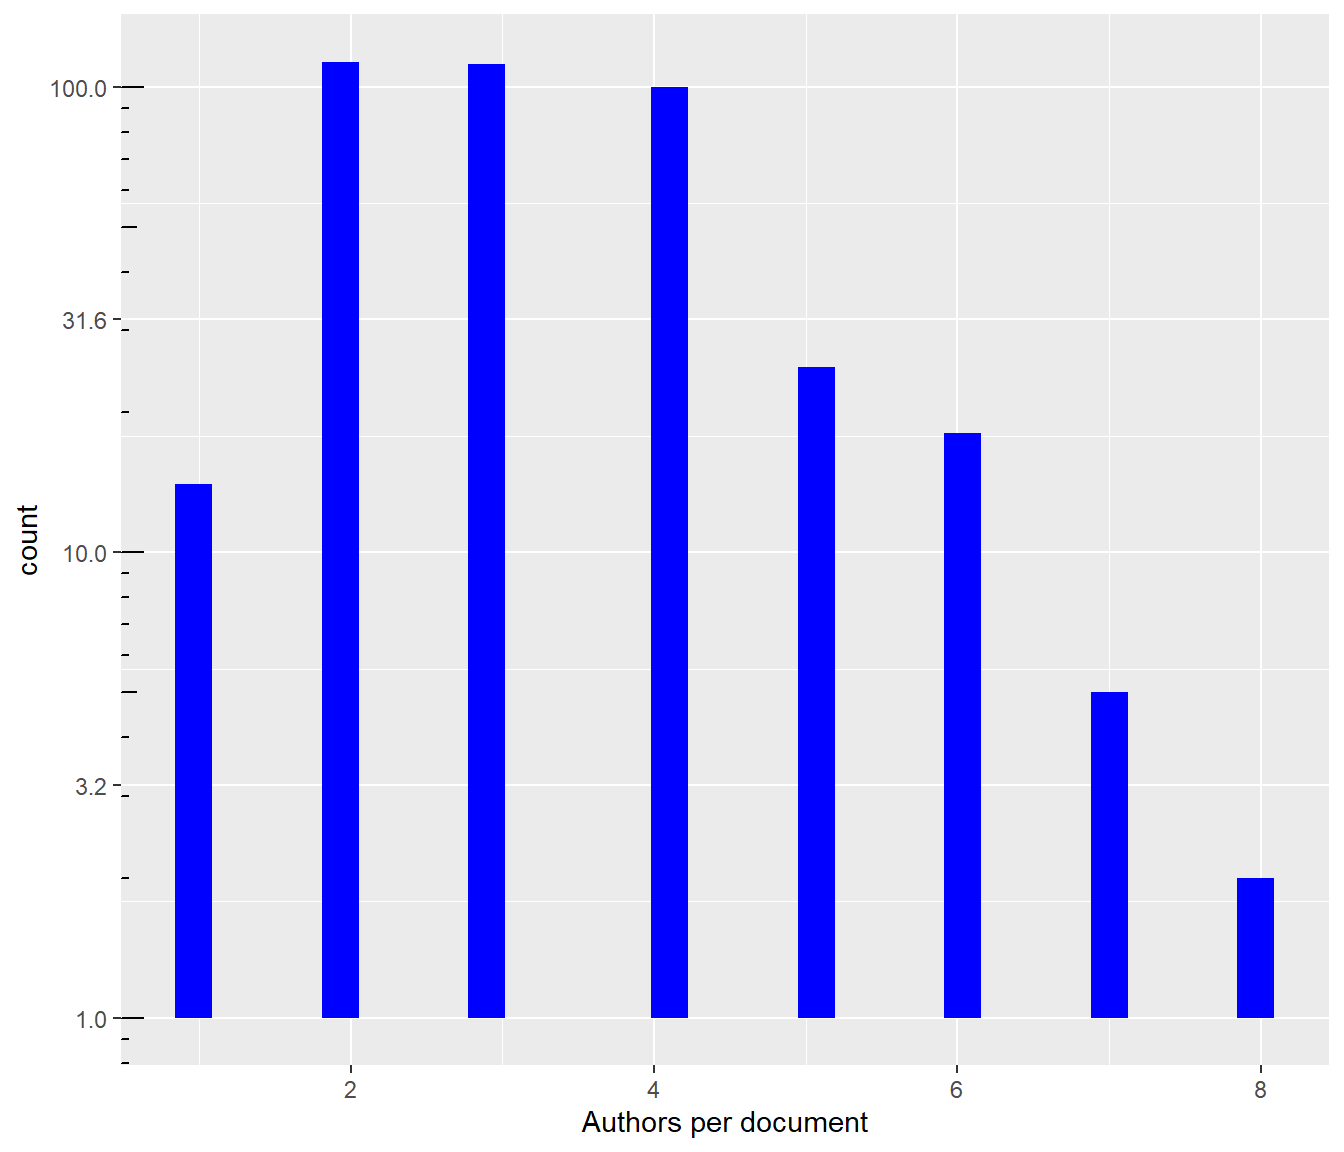
\includegraphics[width=0.7\linewidth]{21-scimetr_files/figure-latex/plotdb-1} \end{center}

\begin{center}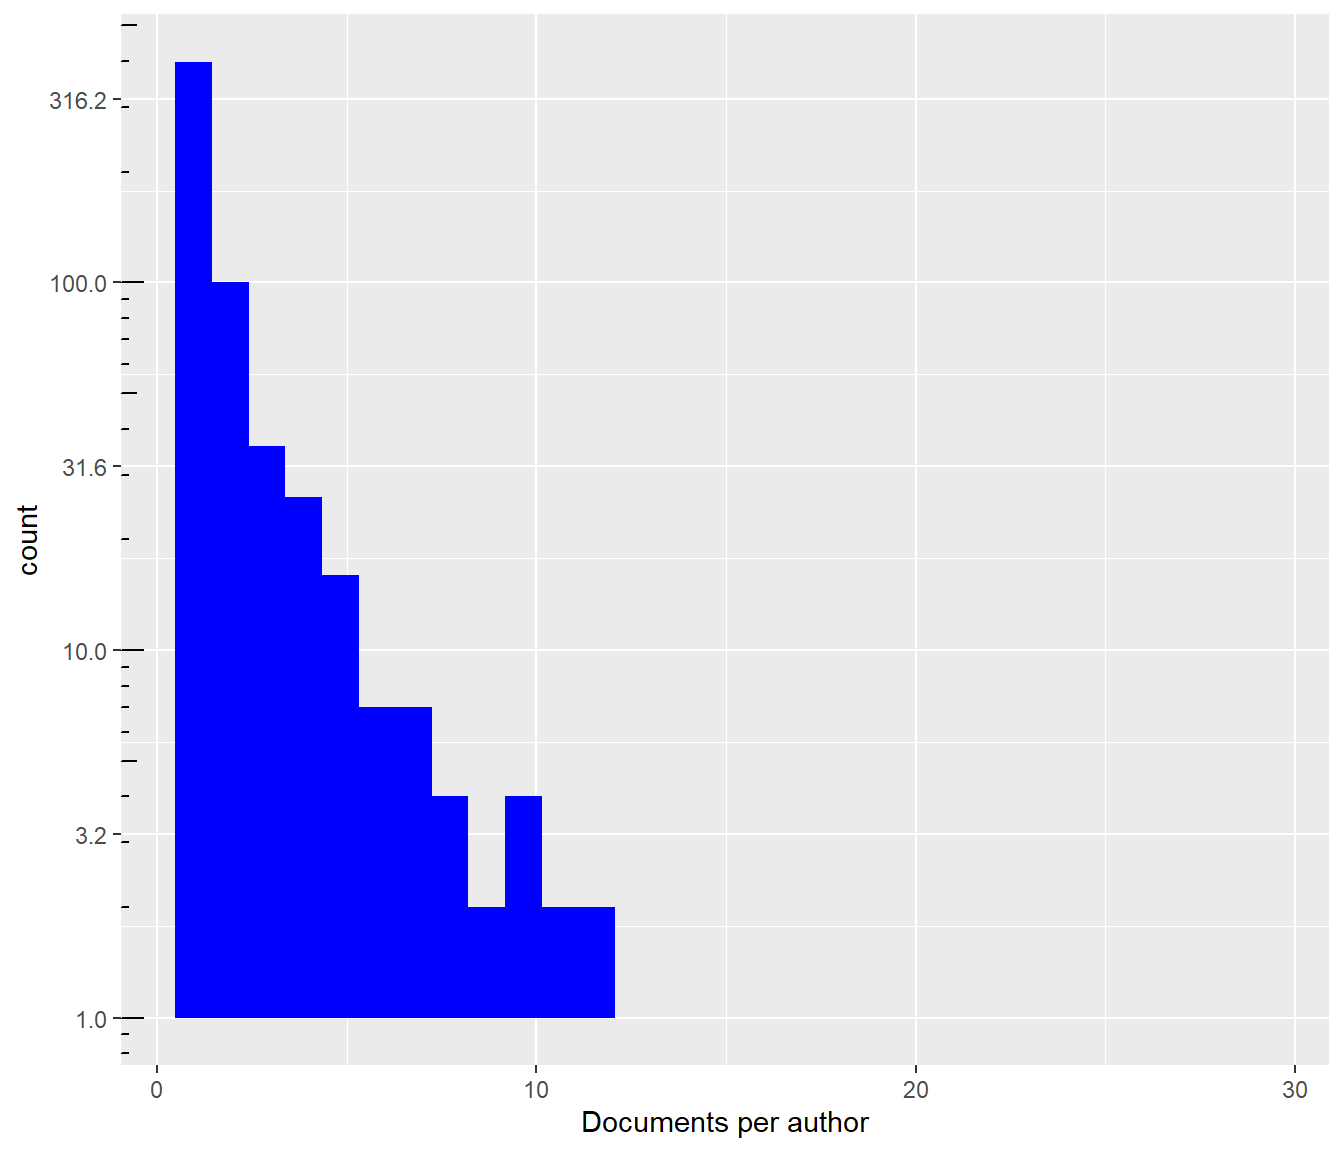
\includegraphics[width=0.7\linewidth]{21-scimetr_files/figure-latex/plotdb-2} \end{center}

\begin{center}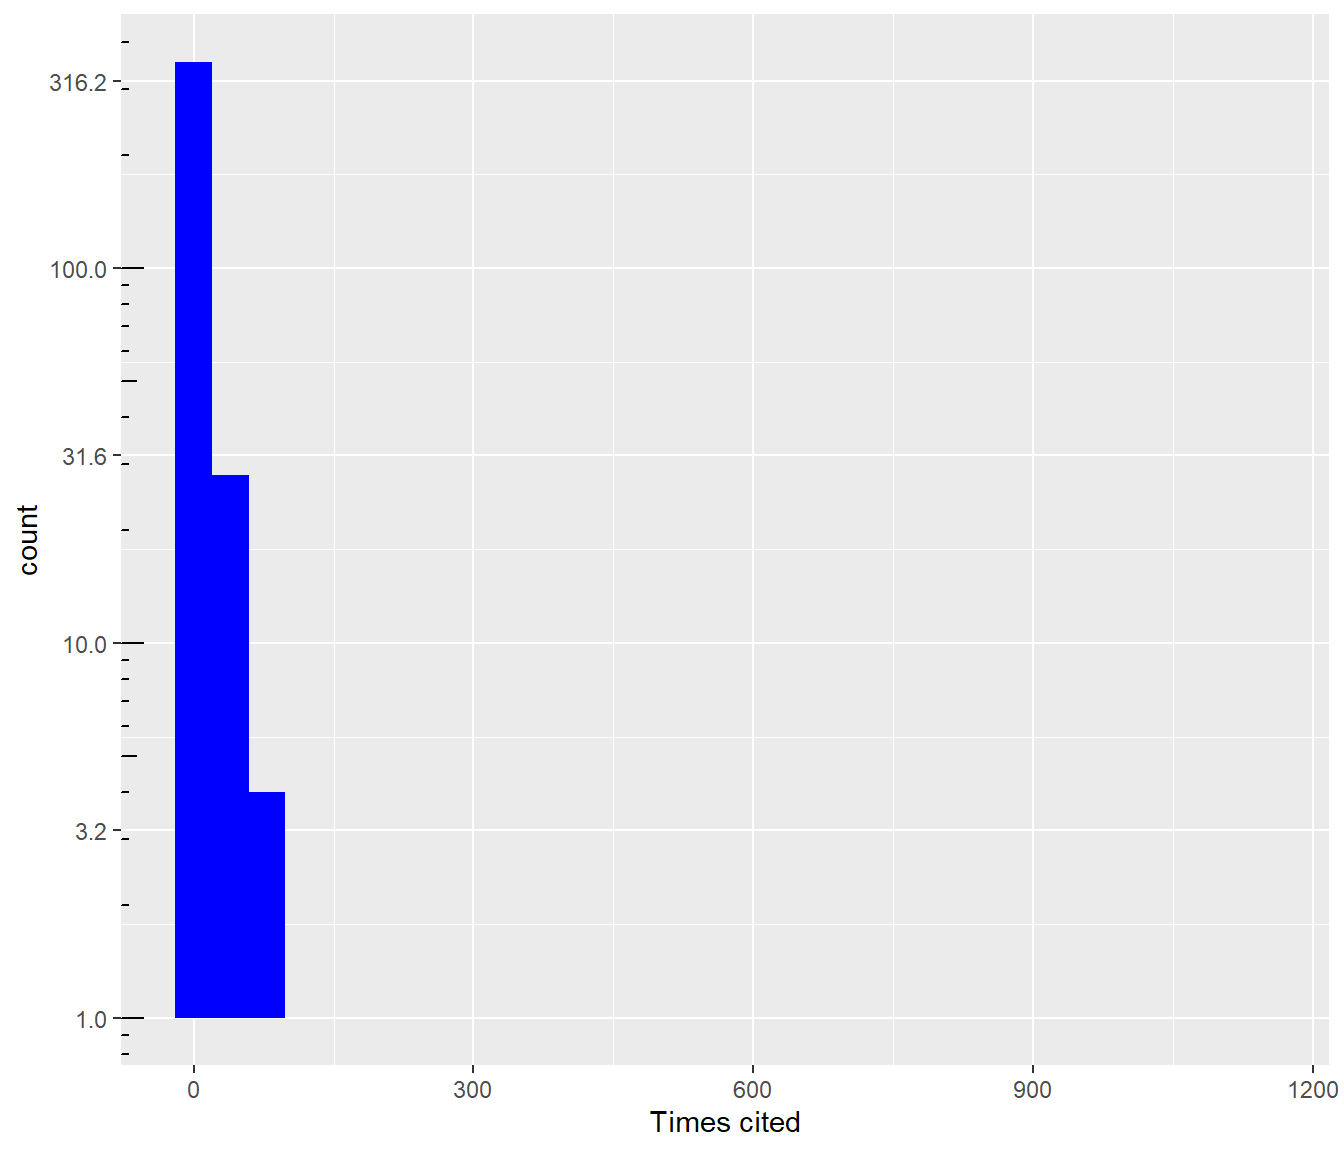
\includegraphics[width=0.7\linewidth]{21-scimetr_files/figure-latex/plotdb-3} \end{center}

\subsection{\texorpdfstring{Gráficos sumario
\texttt{plot.summary.wos.db()}}{Gráficos sumario plot.summary.wos.db()}}\label{gruxe1ficos-sumario-plot.summary.wos.db}

\begin{Shaded}
\begin{Highlighting}[]
\KeywordTok{plot}\NormalTok{(res1)}
\end{Highlighting}
\end{Shaded}

\begin{flushleft}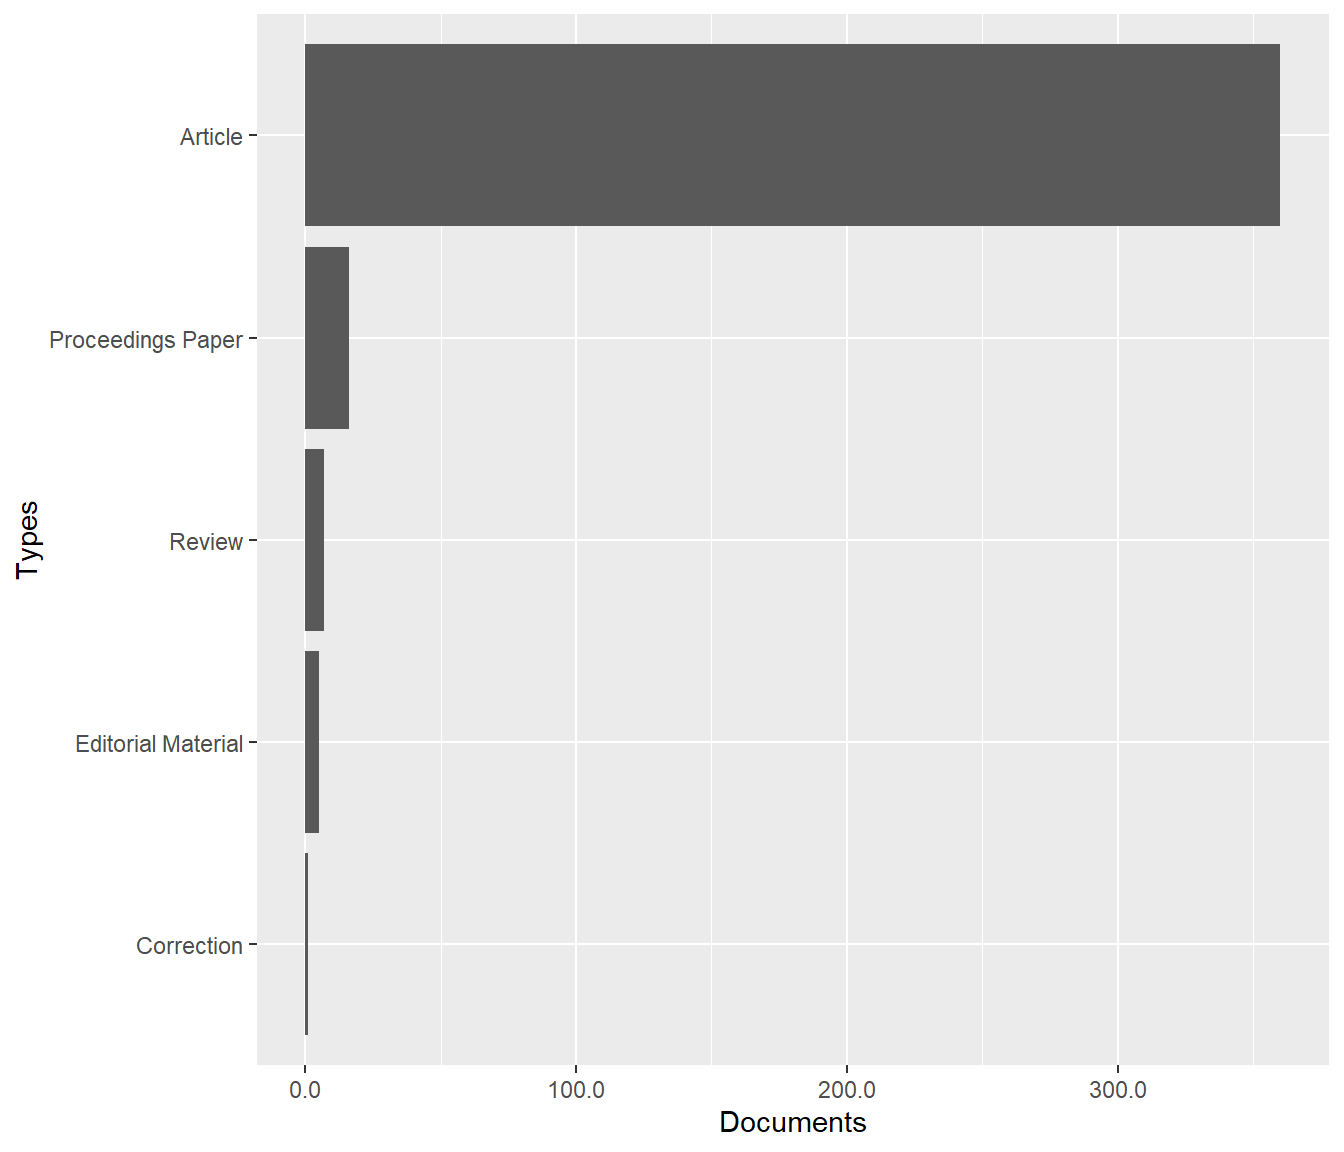
\includegraphics[width=0.7\linewidth]{21-scimetr_files/figure-latex/unnamed-chunk-9-1} \end{flushleft}

\begin{flushleft}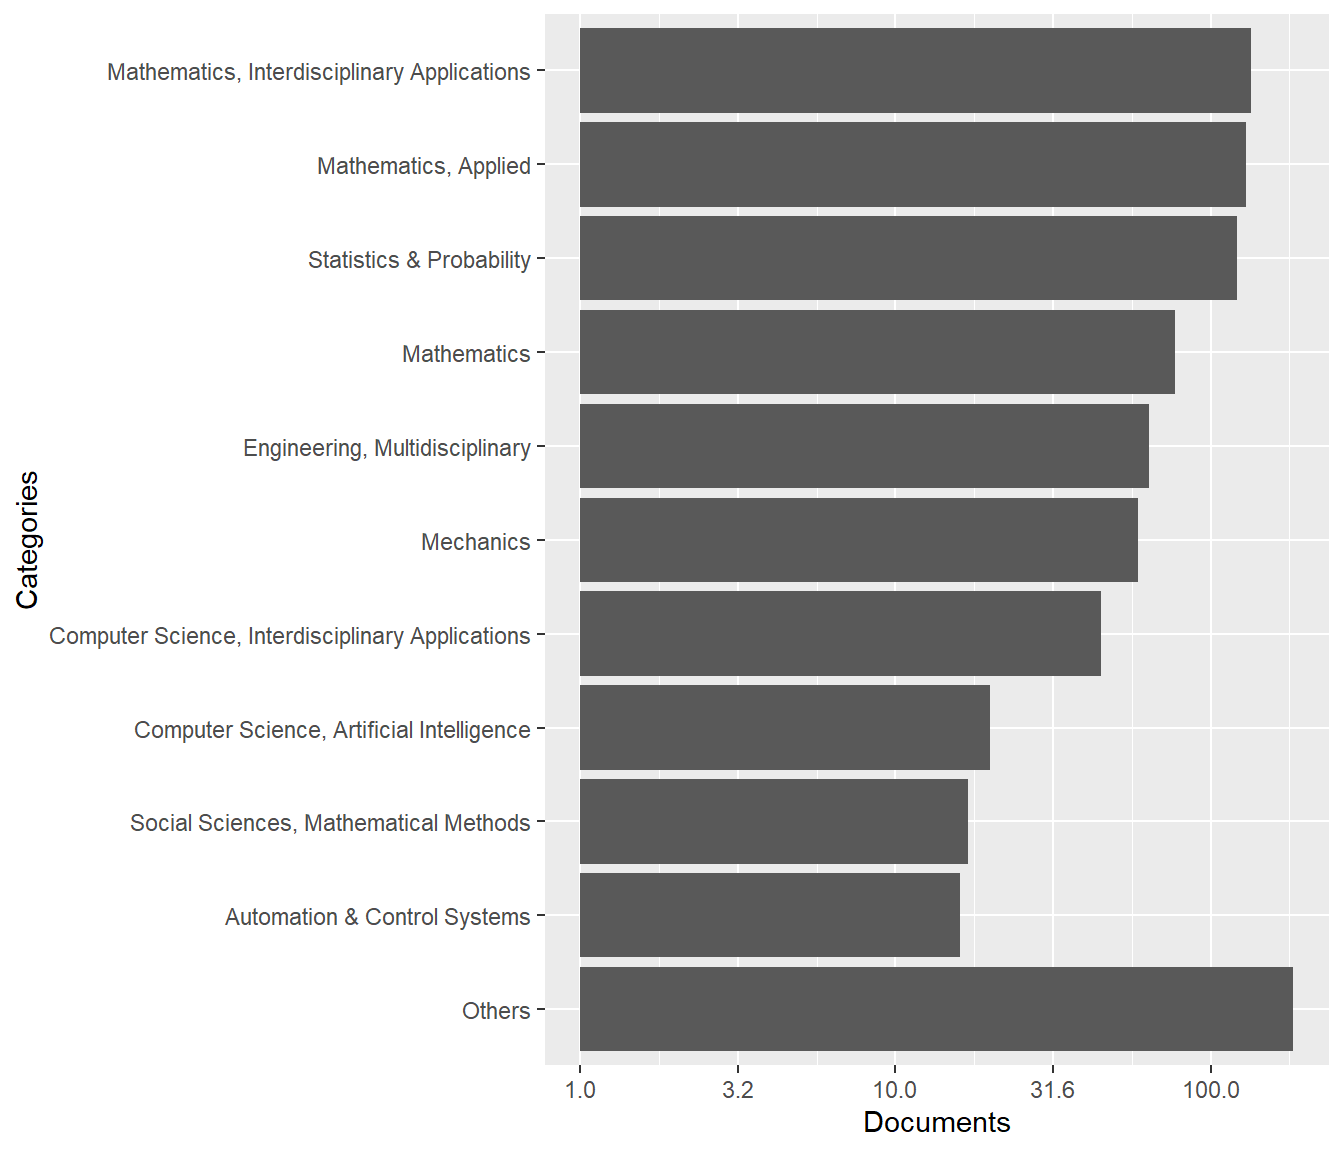
\includegraphics[width=0.7\linewidth]{21-scimetr_files/figure-latex/unnamed-chunk-9-2} \end{flushleft}

\begin{flushleft}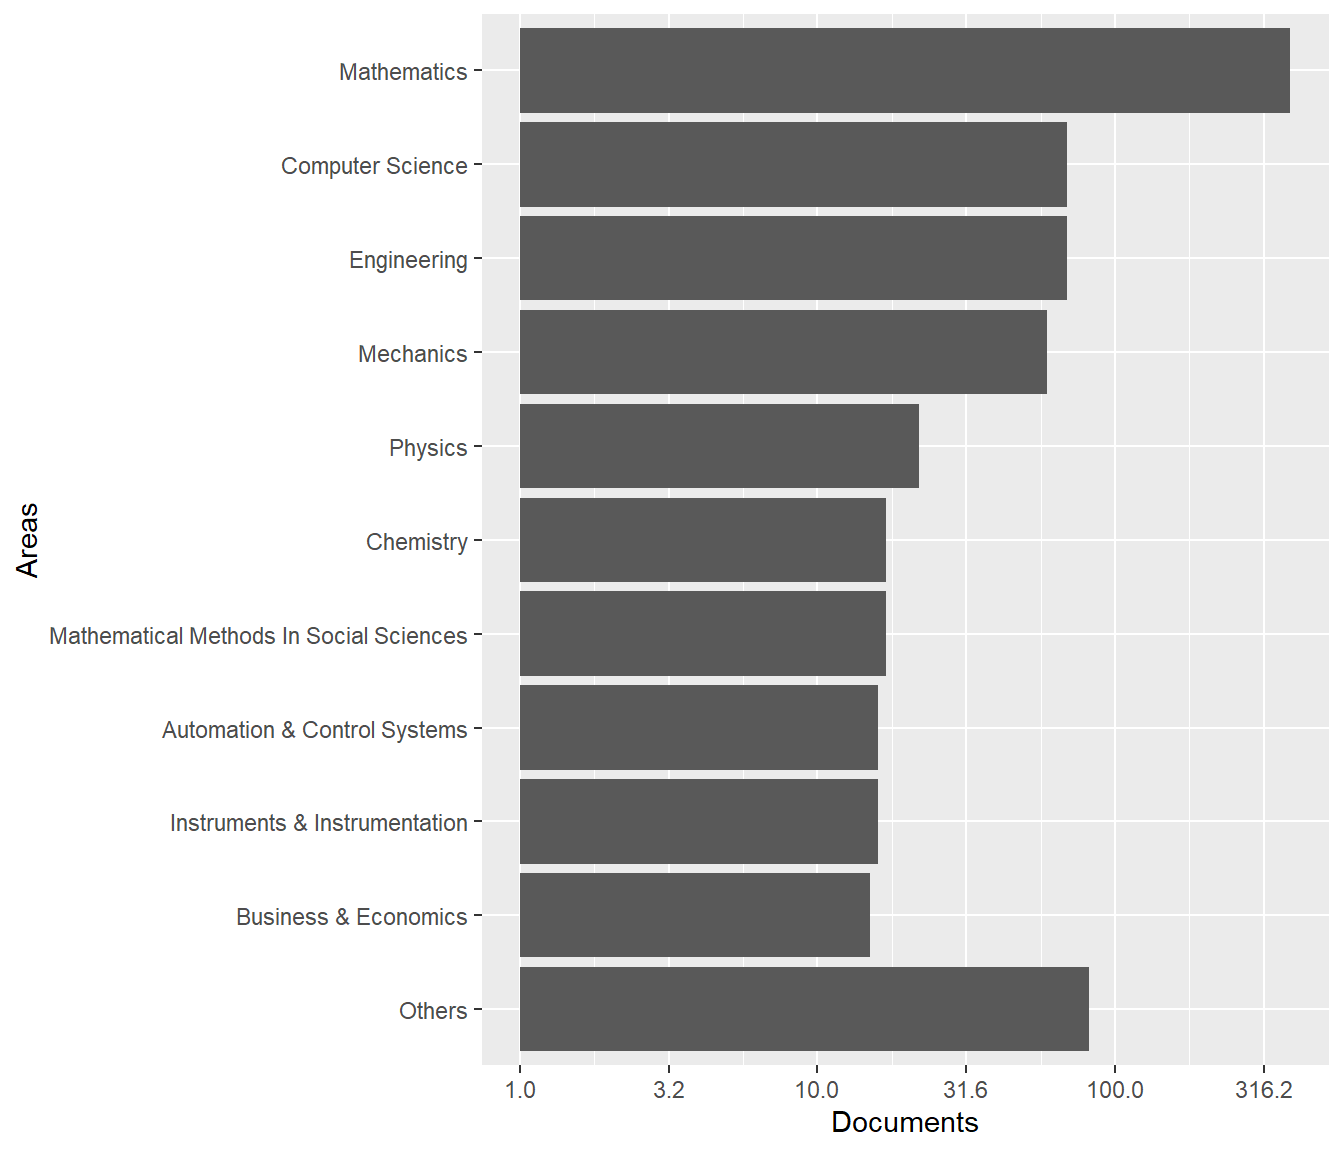
\includegraphics[width=0.7\linewidth]{21-scimetr_files/figure-latex/unnamed-chunk-9-3} \end{flushleft}

\begin{flushleft}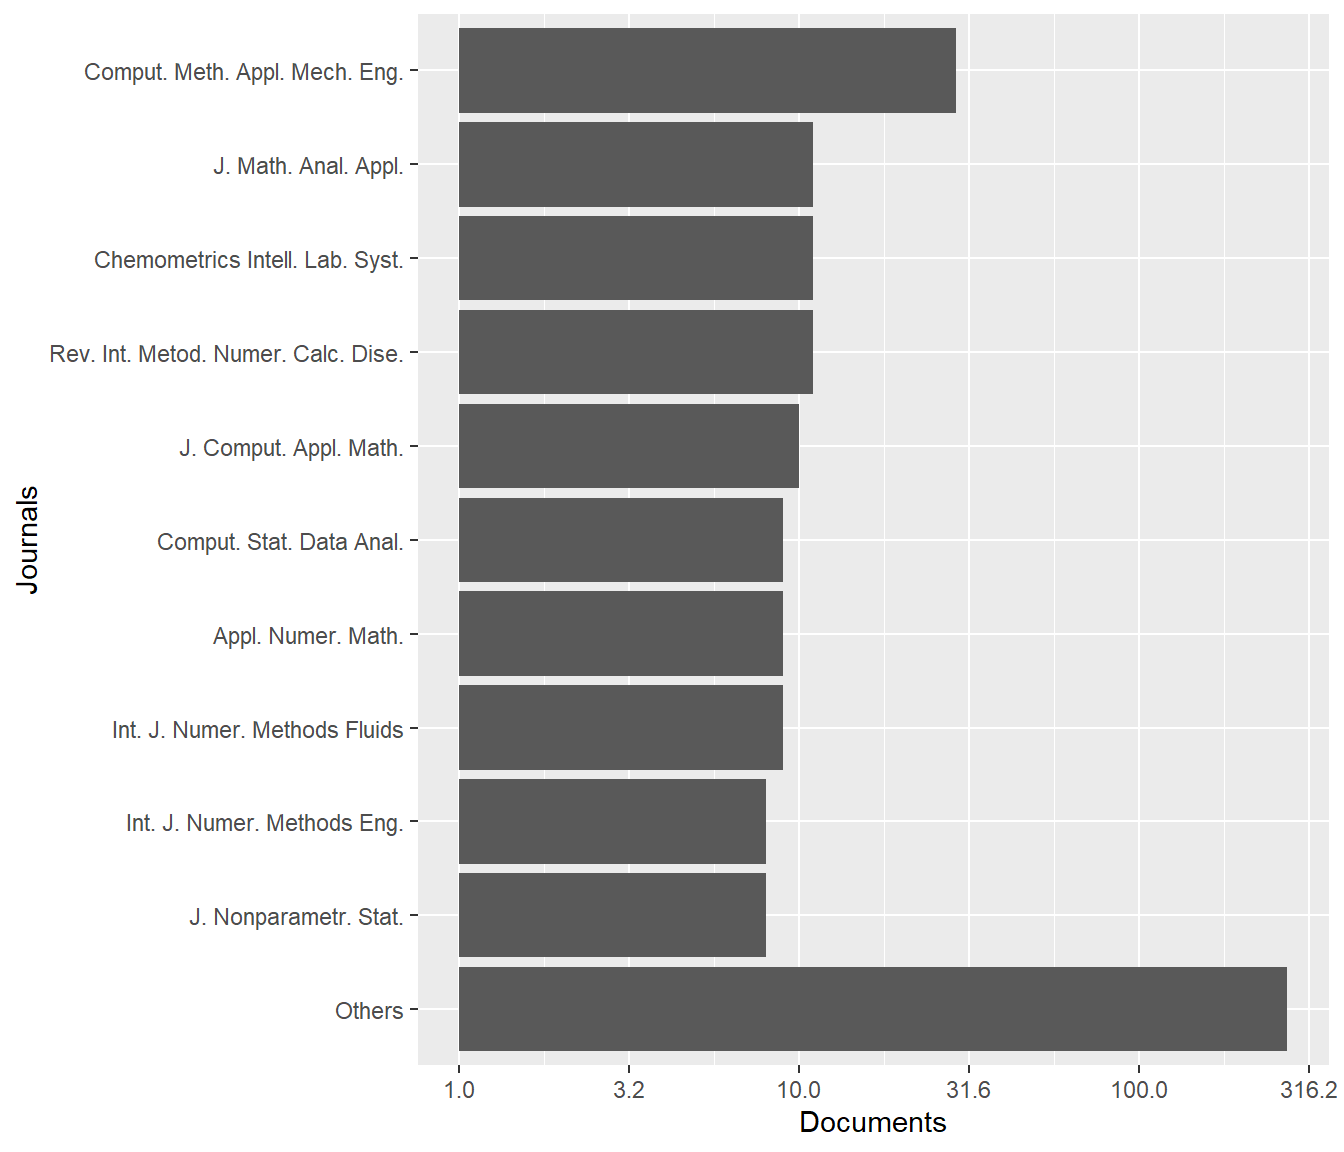
\includegraphics[width=0.7\linewidth]{21-scimetr_files/figure-latex/unnamed-chunk-9-4} \end{flushleft}

\begin{flushleft}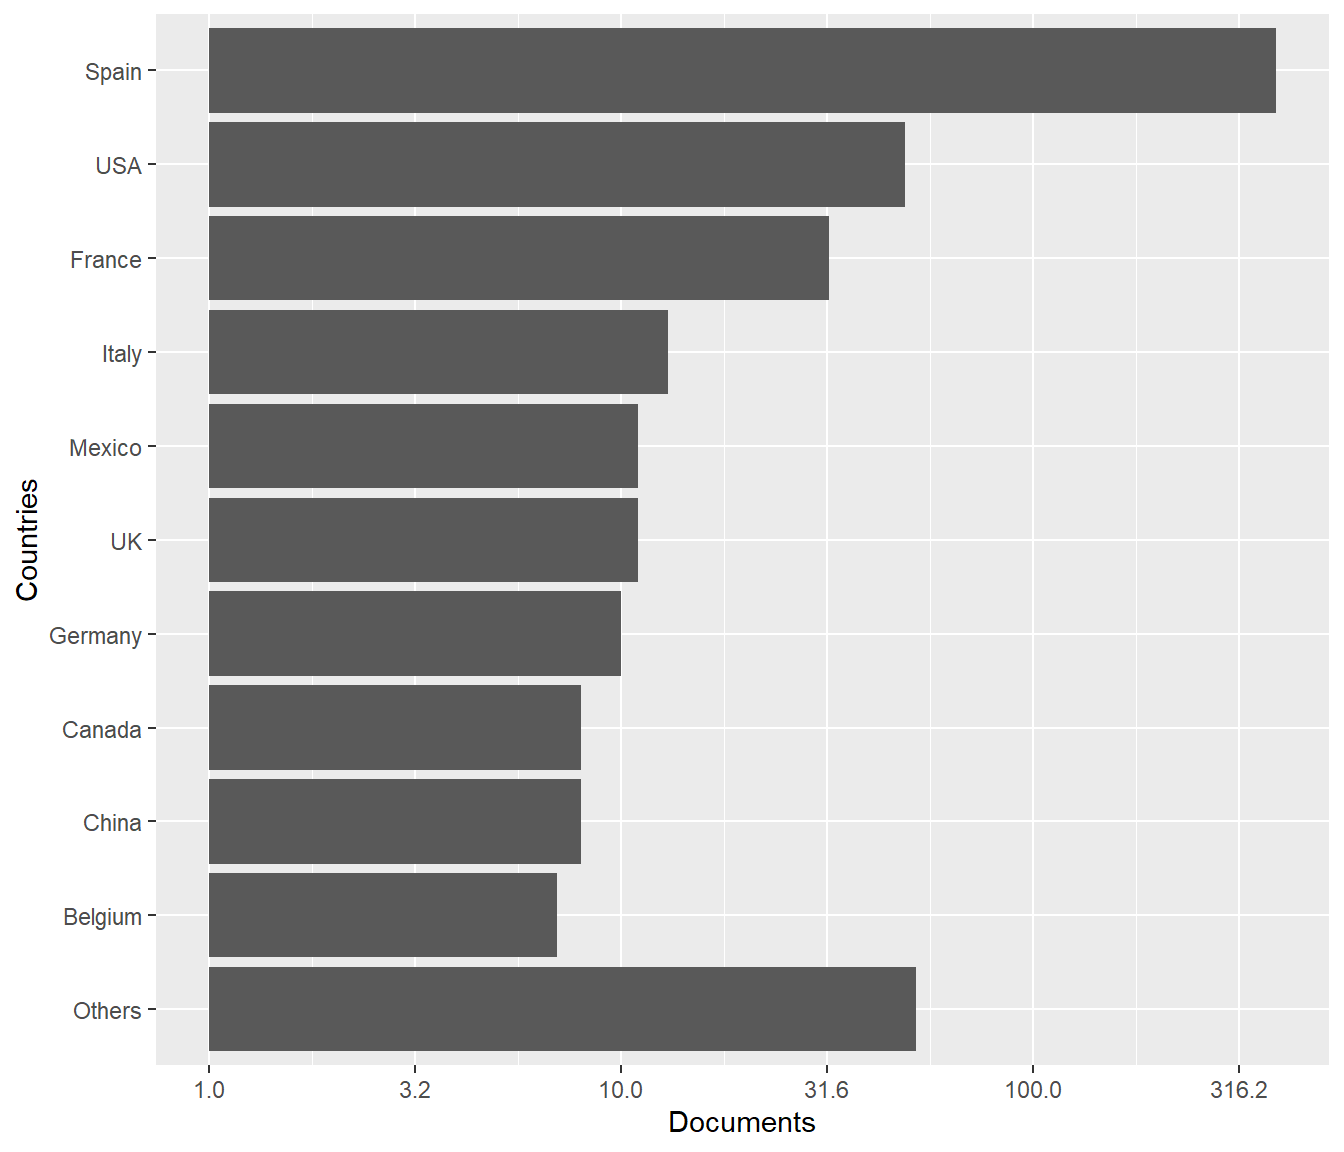
\includegraphics[width=0.7\linewidth]{21-scimetr_files/figure-latex/unnamed-chunk-9-5} \end{flushleft}

\begin{Shaded}
\begin{Highlighting}[]
\KeywordTok{plot}\NormalTok{(res1, }\DataTypeTok{pie =} \OtherTok{TRUE}\NormalTok{)}
\end{Highlighting}
\end{Shaded}

\begin{flushleft}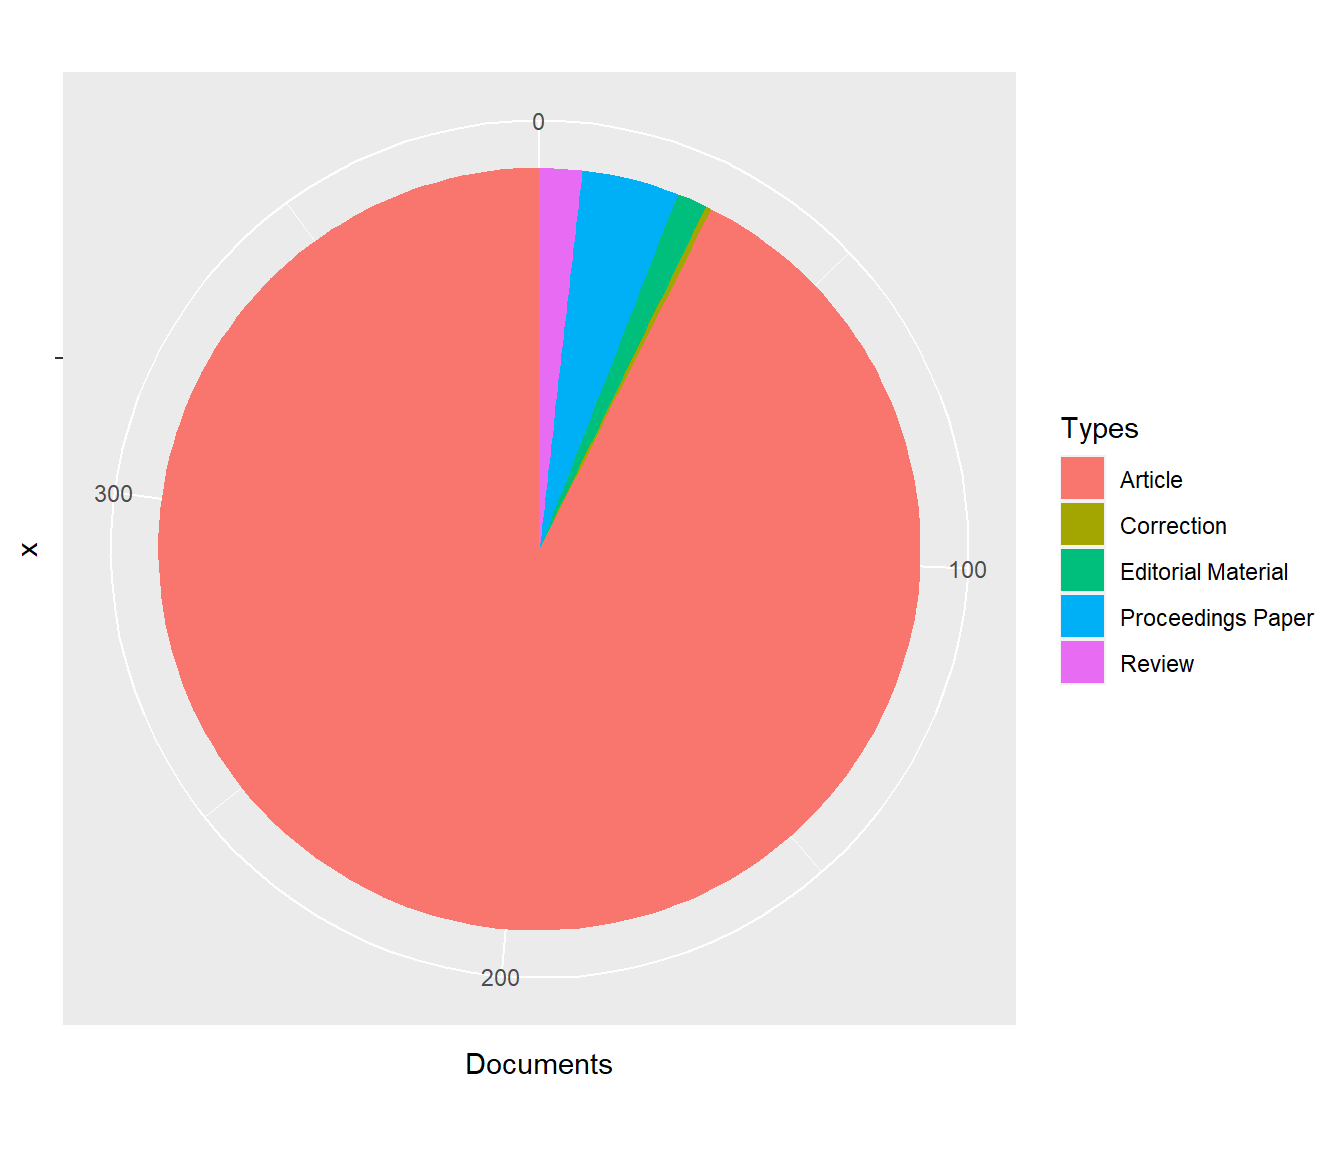
\includegraphics[width=0.7\linewidth]{21-scimetr_files/figure-latex/unnamed-chunk-9-6} \end{flushleft}

\begin{flushleft}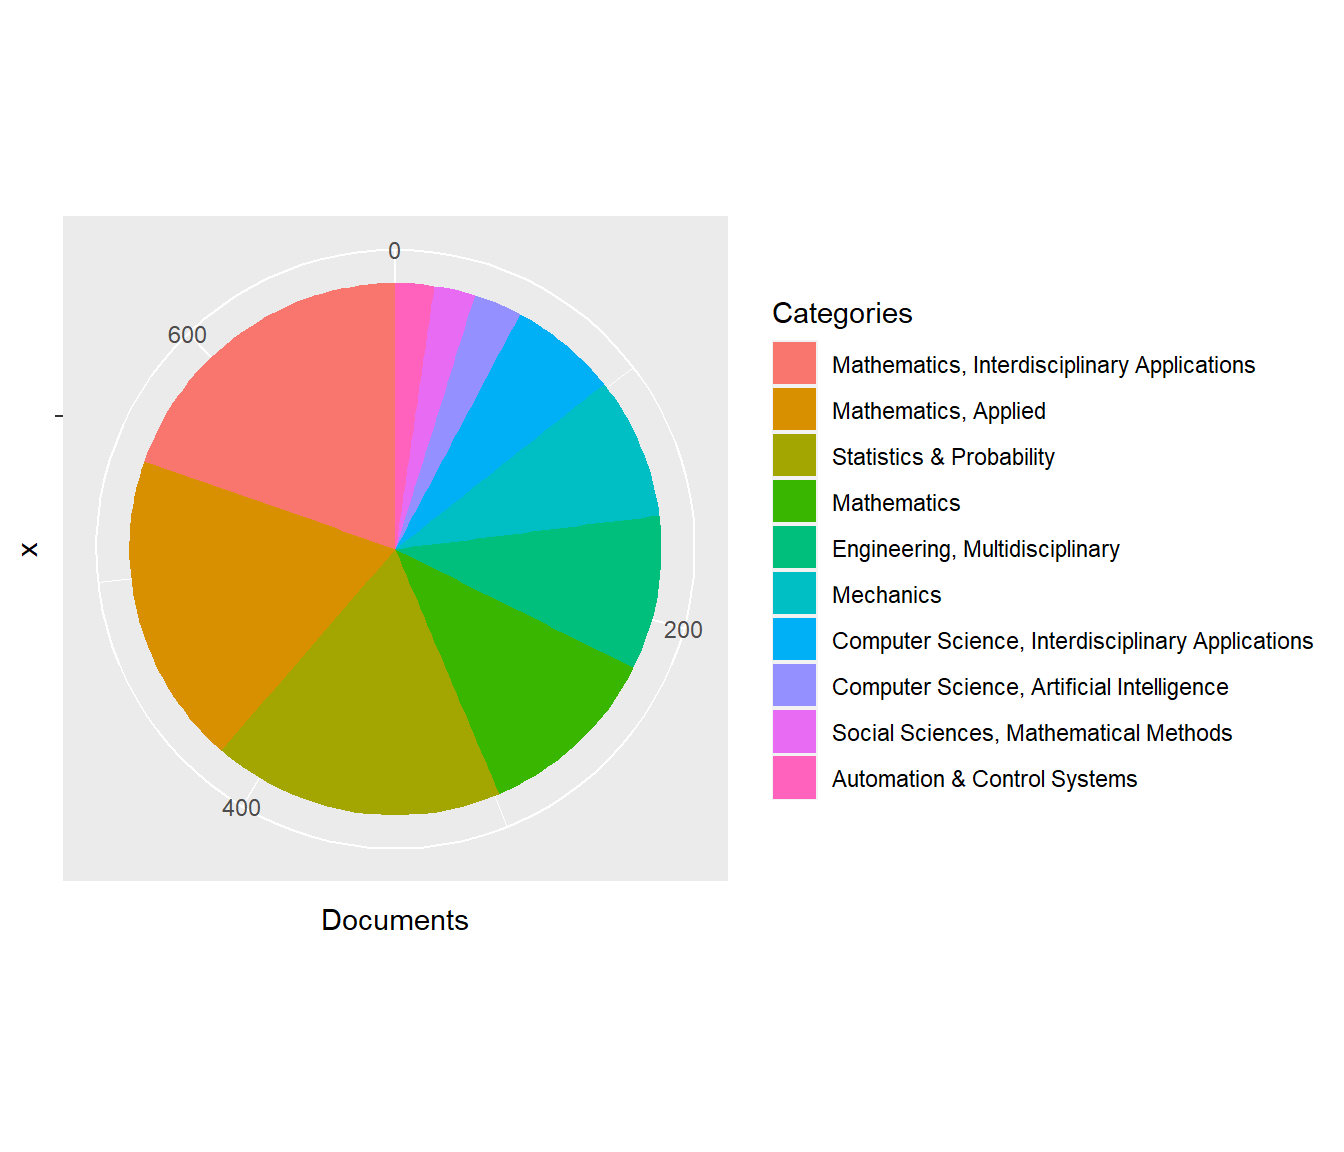
\includegraphics[width=0.7\linewidth]{21-scimetr_files/figure-latex/unnamed-chunk-9-7} \end{flushleft}

\begin{flushleft}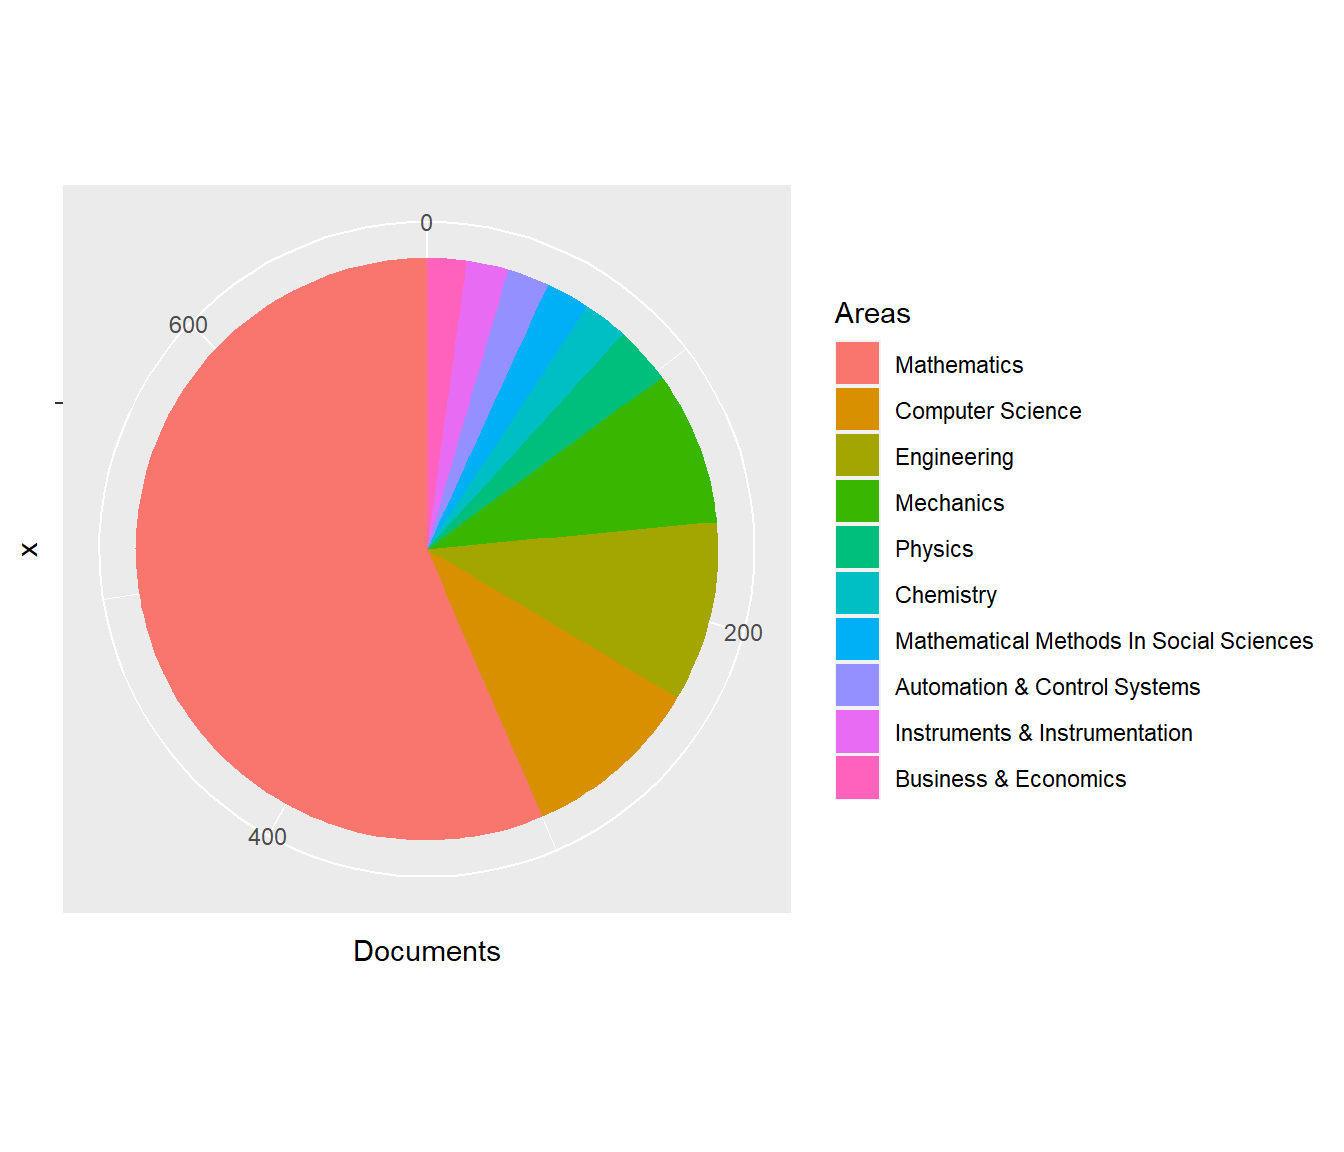
\includegraphics[width=0.7\linewidth]{21-scimetr_files/figure-latex/unnamed-chunk-9-8} \end{flushleft}

\begin{flushleft}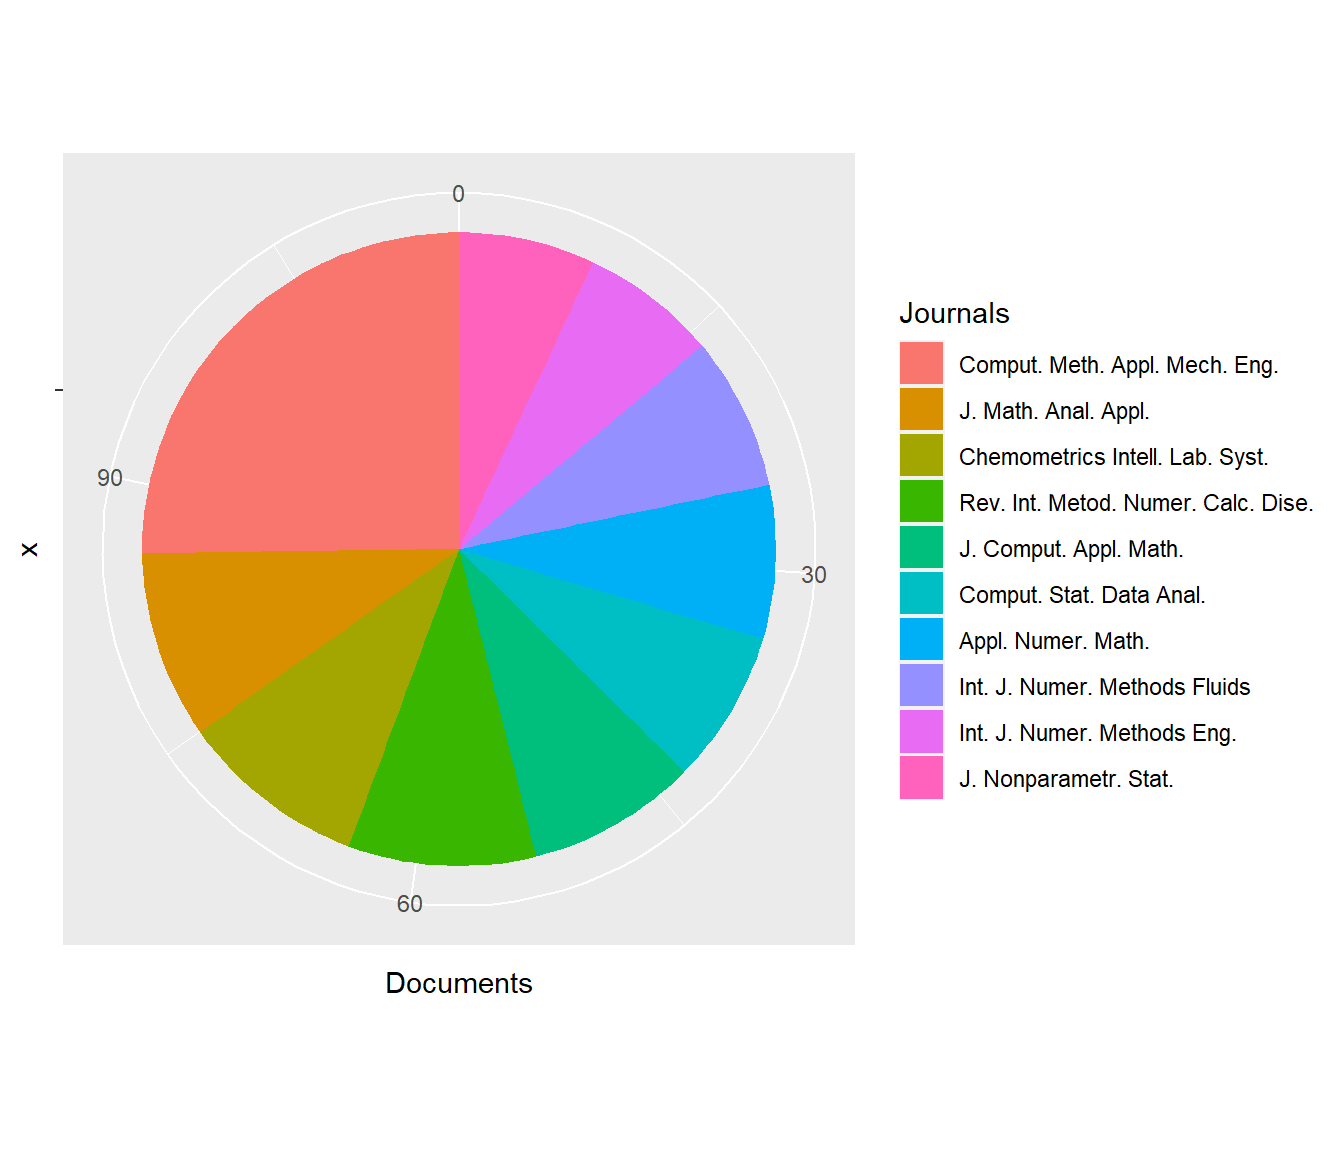
\includegraphics[width=0.7\linewidth]{21-scimetr_files/figure-latex/unnamed-chunk-9-9} \end{flushleft}

\begin{flushleft}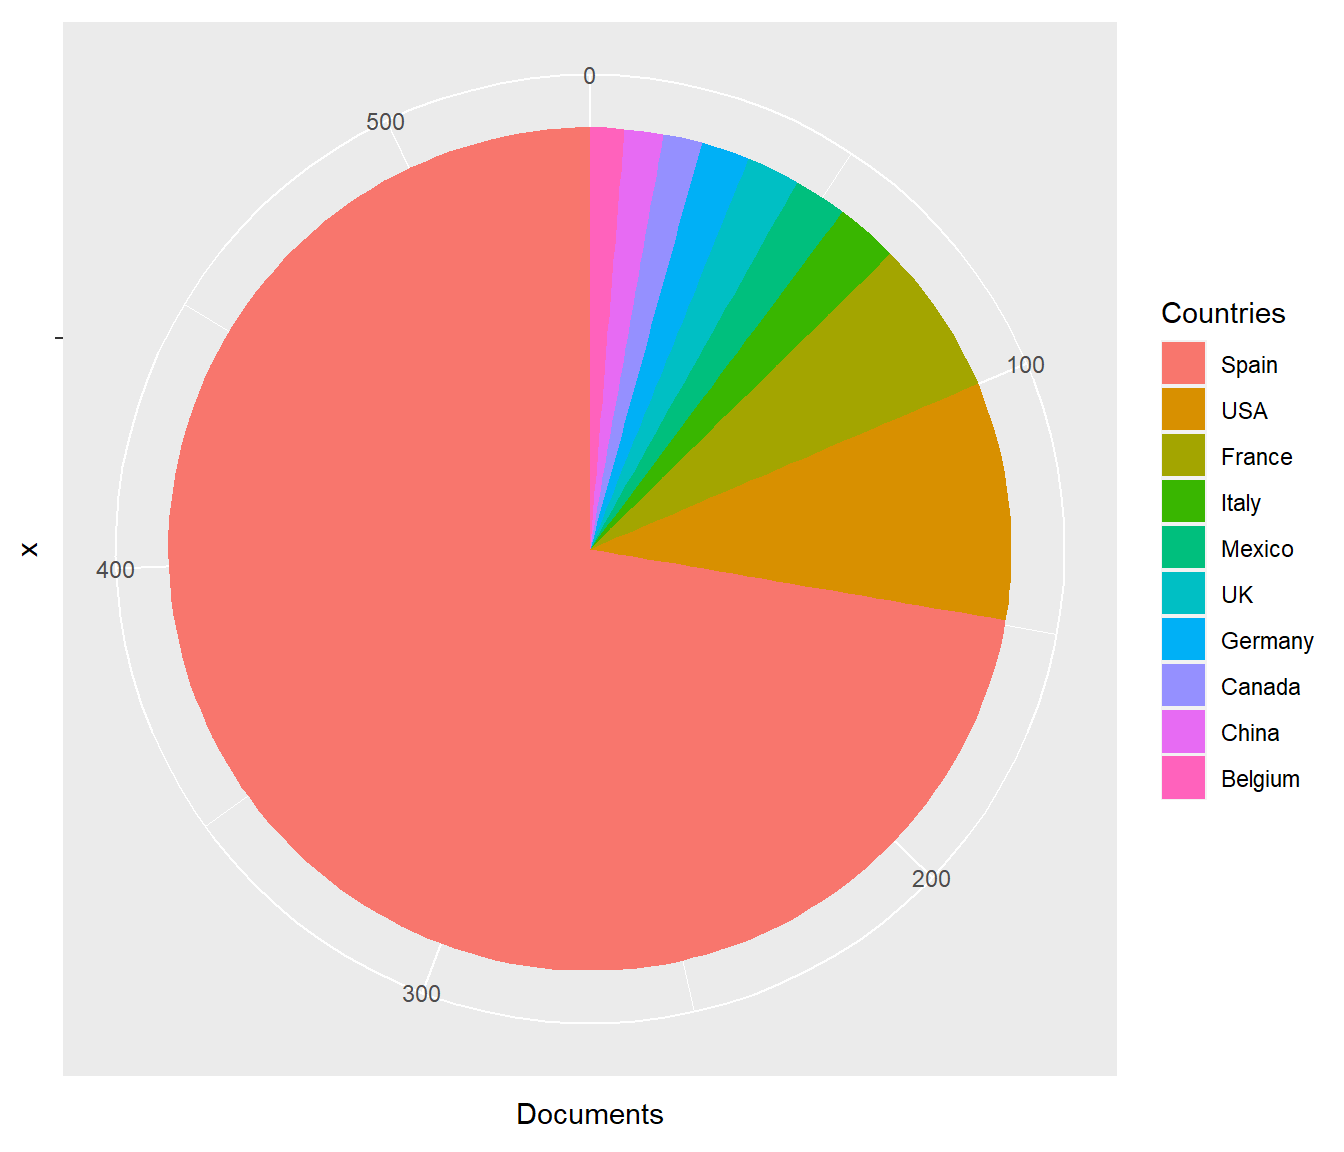
\includegraphics[width=0.7\linewidth]{21-scimetr_files/figure-latex/unnamed-chunk-9-10} \end{flushleft}

\subsection{\texorpdfstring{Gráficos sumario por años
\texttt{plot.summary.year()}}{Gráficos sumario por años plot.summary.year()}}\label{gruxe1ficos-sumario-por-auxf1os-plot.summary.year}

\begin{Shaded}
\begin{Highlighting}[]
\KeywordTok{plot}\NormalTok{(res2)}
\end{Highlighting}
\end{Shaded}

\begin{flushleft}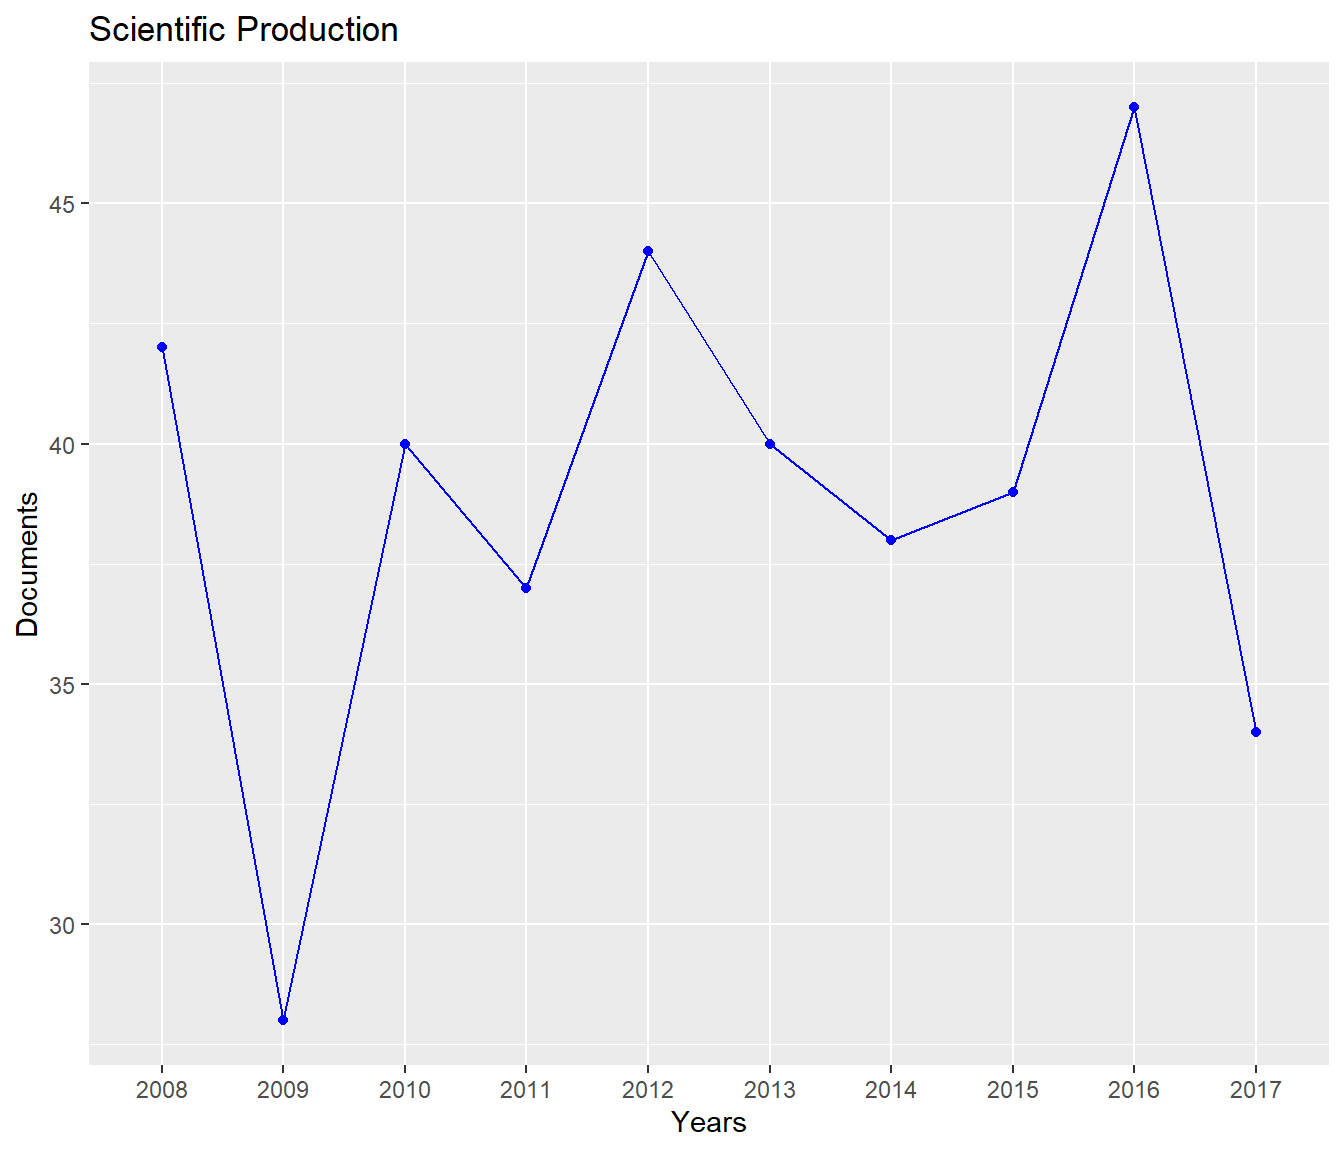
\includegraphics[width=0.7\linewidth]{21-scimetr_files/figure-latex/unnamed-chunk-10-1} \end{flushleft}

\begin{flushleft}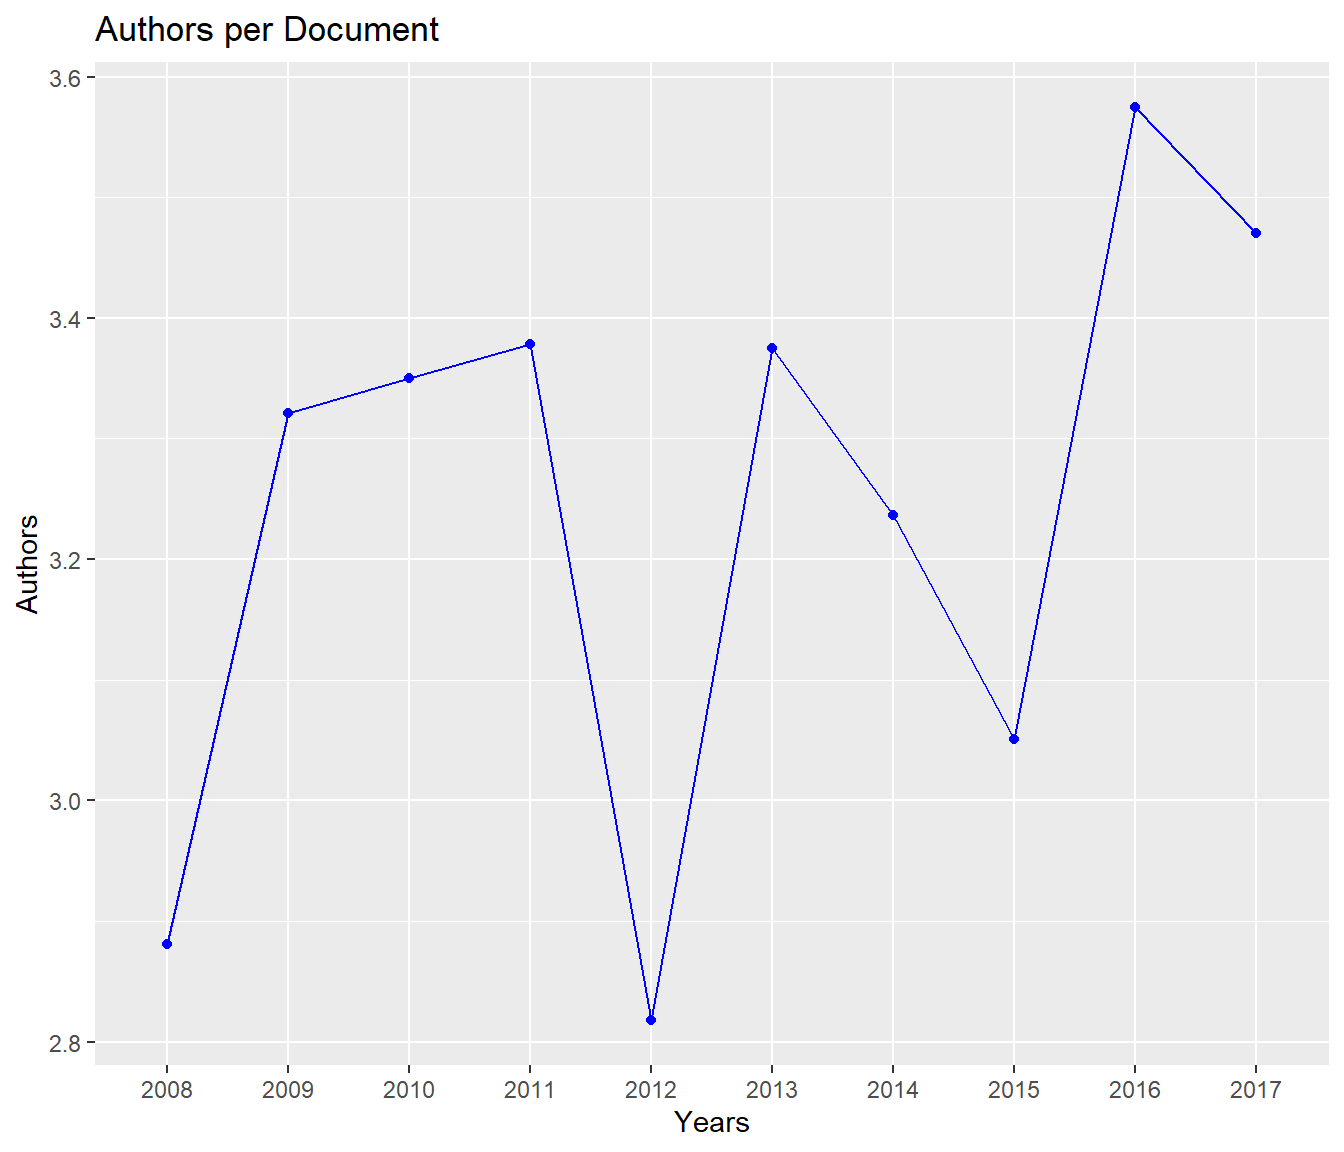
\includegraphics[width=0.7\linewidth]{21-scimetr_files/figure-latex/unnamed-chunk-10-2} \end{flushleft}

\begin{flushleft}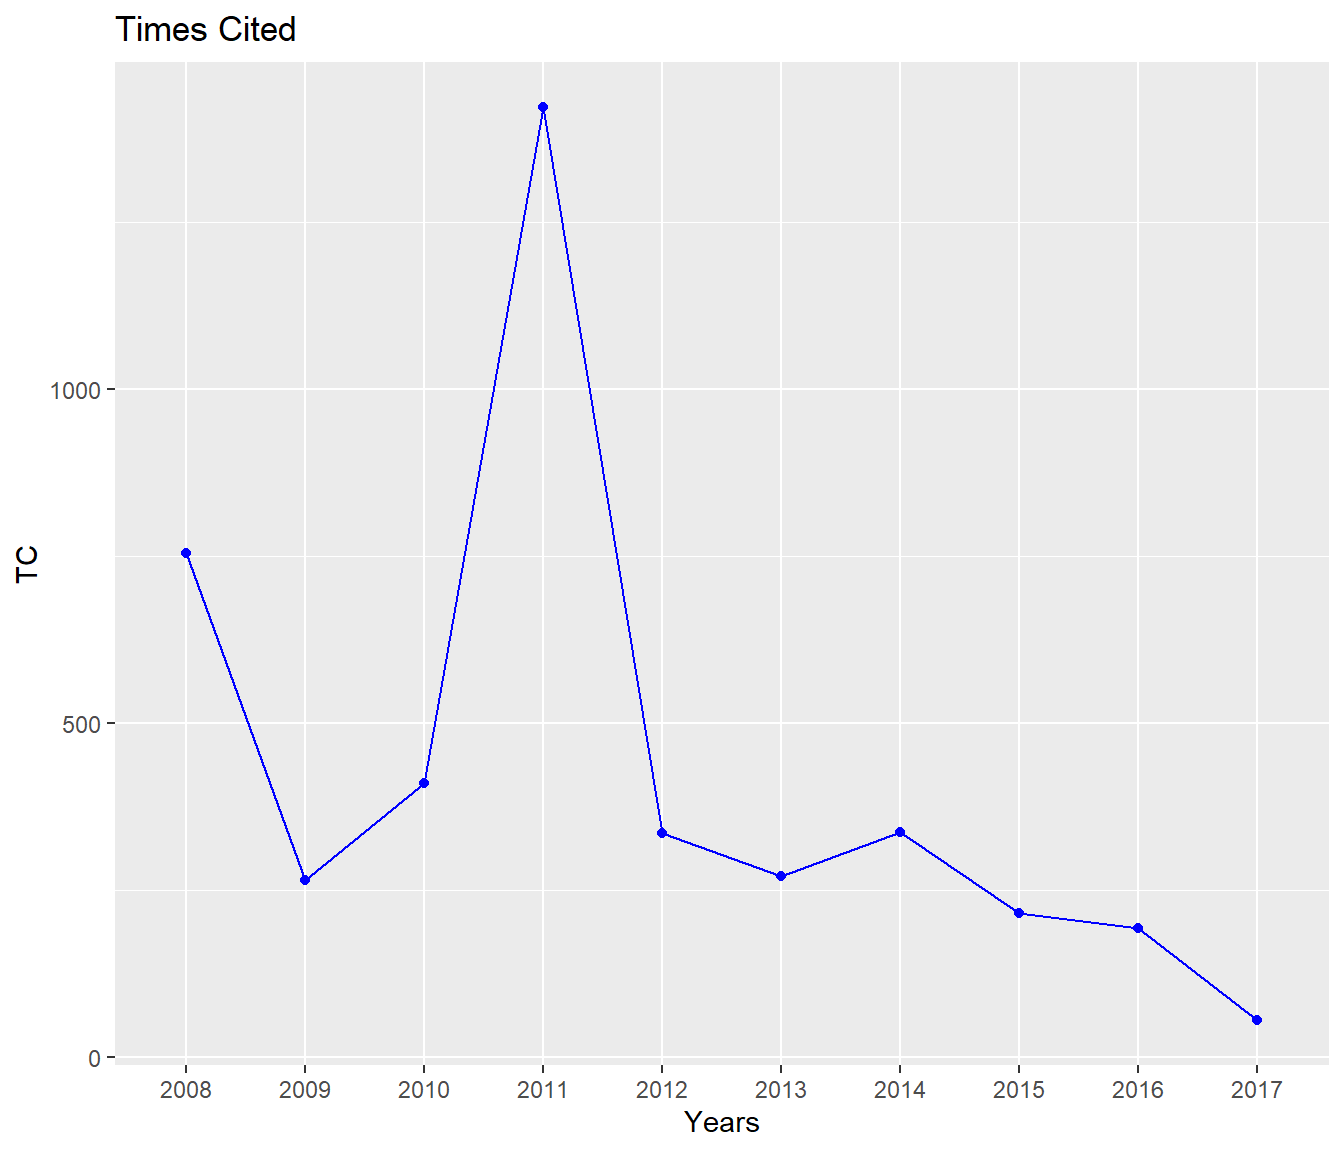
\includegraphics[width=0.7\linewidth]{21-scimetr_files/figure-latex/unnamed-chunk-10-3} \end{flushleft}

\begin{Shaded}
\begin{Highlighting}[]
\KeywordTok{plot}\NormalTok{(res2, }\DataTypeTok{boxplot =} \OtherTok{TRUE}\NormalTok{)}
\end{Highlighting}
\end{Shaded}

\begin{flushleft}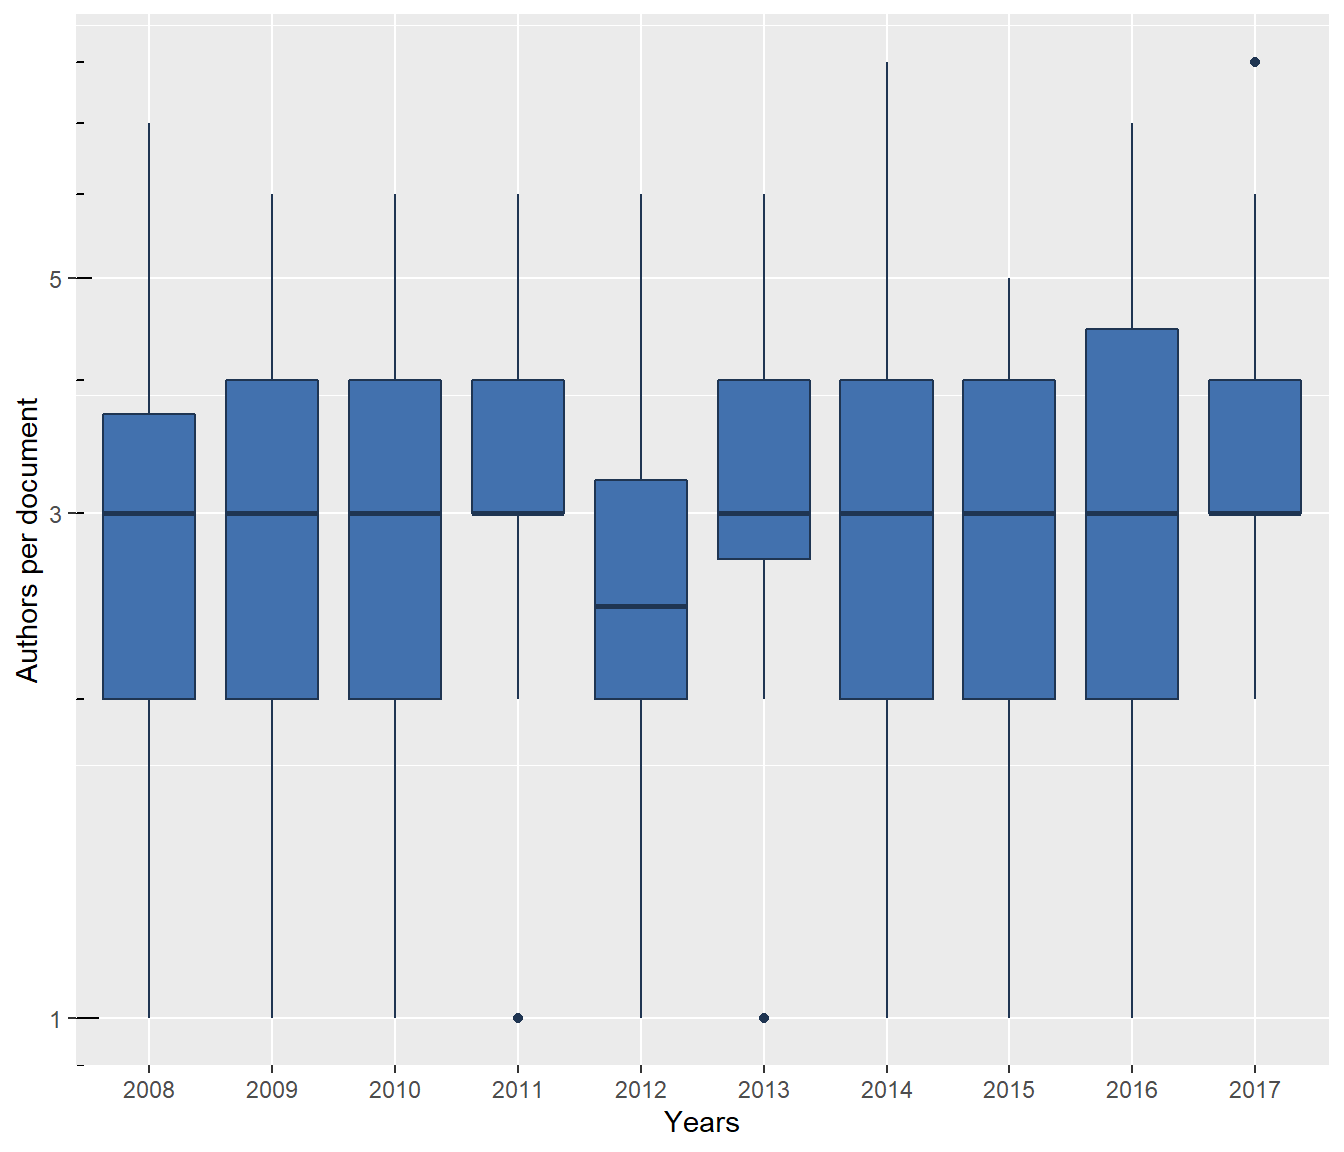
\includegraphics[width=0.7\linewidth]{21-scimetr_files/figure-latex/unnamed-chunk-10-4} \end{flushleft}

\begin{flushleft}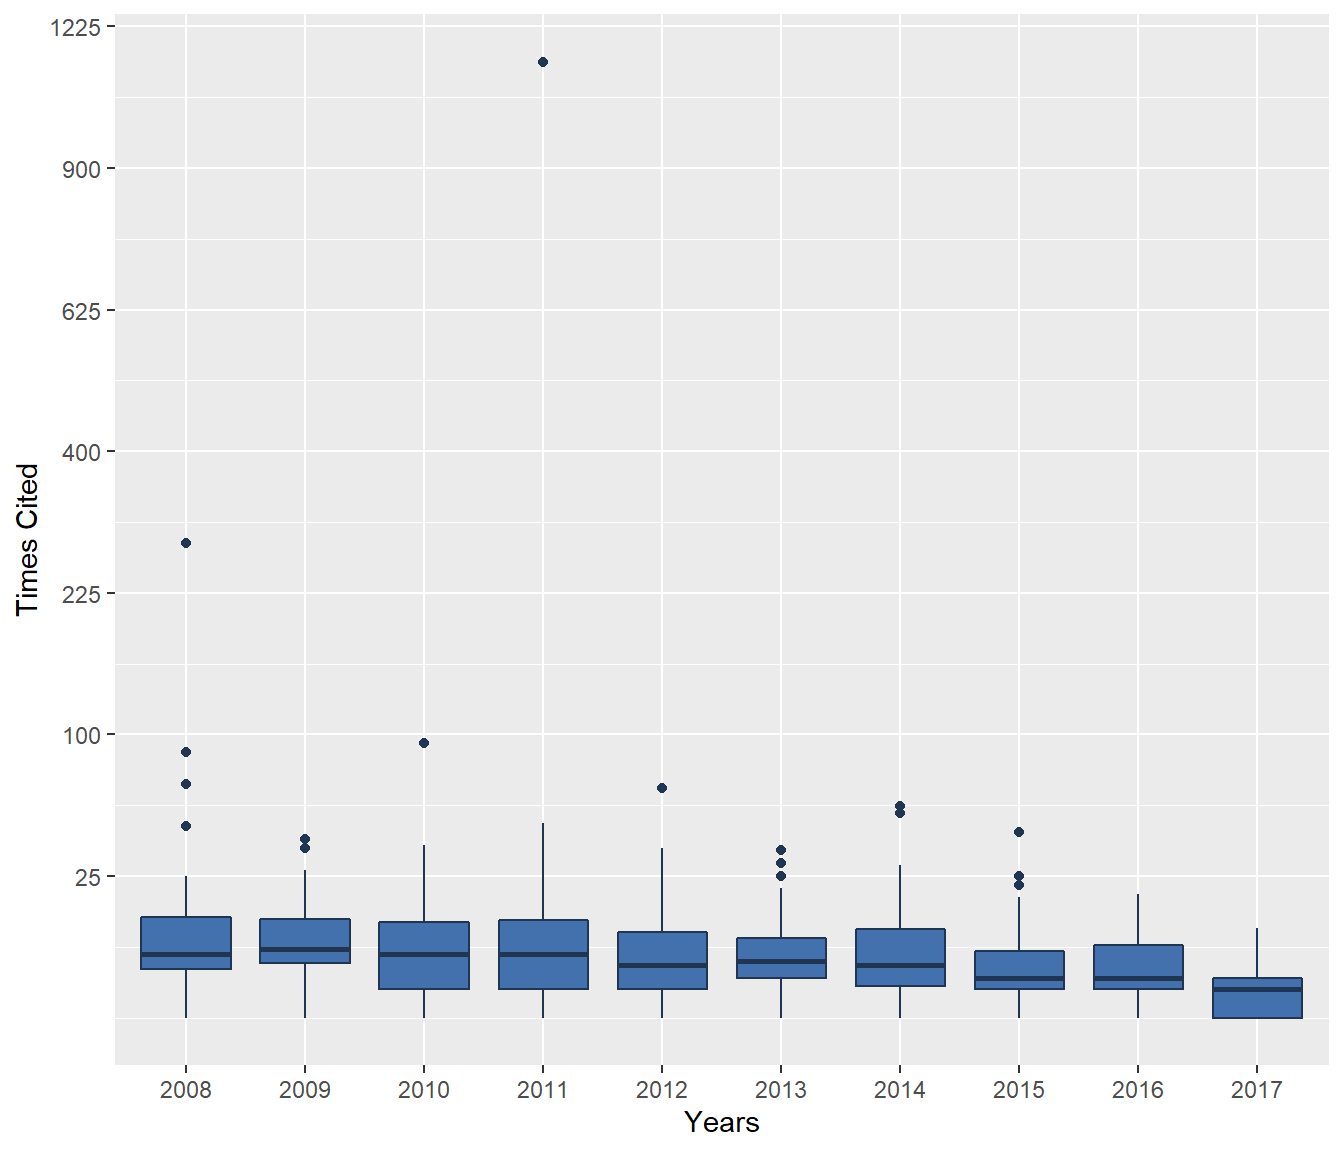
\includegraphics[width=0.7\linewidth]{21-scimetr_files/figure-latex/unnamed-chunk-10-5} \end{flushleft}

\section{Filtrado}\label{filtrado-1}

Se combinan las funciones
\texttt{get.id\textless{}Tabla\textgreater{}()} (se puede emplear
cualquier variable de la correspondiente tabla; multiple conditions are
combined with \texttt{\&}, see e.g. \texttt{dplyr::filter()}) con la
función \texttt{get.idDocs()}.

\subsection{Funciones get}\label{funciones-get}

\begin{itemize}
\item
  \texttt{get.idAuthors()}: buscar id (códigos) de autores

  Buscar un autor concreto:

\begin{Shaded}
\begin{Highlighting}[]
\NormalTok{idAuthor <-}\StringTok{ }\KeywordTok{get.idAuthors}\NormalTok{(db, AF }\OperatorTok{==}\StringTok{ "Cao, Ricardo"}\NormalTok{)}
\NormalTok{idAuthor}
\end{Highlighting}
\end{Shaded}

\begin{verbatim}
## Cao, Ricardo 
##           16
\end{verbatim}

  Buscar en nombres de autores:

\begin{Shaded}
\begin{Highlighting}[]
\NormalTok{idAuthors <-}\StringTok{ }\KeywordTok{get.idAuthors}\NormalTok{(db, }\KeywordTok{grepl}\NormalTok{(}\StringTok{'Cao'}\NormalTok{, AF))}
\NormalTok{idAuthors}
\end{Highlighting}
\end{Shaded}

\begin{verbatim}
##           Cao, Ricardo Cao-Rial, Maria Teresa 
##                     16                     69
\end{verbatim}
\item
  \texttt{get.idAreas()}: Devuelve códigos de las áreas

\begin{Shaded}
\begin{Highlighting}[]
\KeywordTok{get.idAreas}\NormalTok{(db, SC }\OperatorTok{==}\StringTok{ 'Mathematics'}\NormalTok{)}
\end{Highlighting}
\end{Shaded}

\begin{verbatim}
## Mathematics 
##          16
\end{verbatim}

\begin{Shaded}
\begin{Highlighting}[]
\KeywordTok{get.idAreas}\NormalTok{(db, SC }\OperatorTok{==}\StringTok{ 'Mathematics'} \OperatorTok{|}\StringTok{ }\NormalTok{SC }\OperatorTok{==}\StringTok{ 'Computer Science'}\NormalTok{)}
\end{Highlighting}
\end{Shaded}

\begin{verbatim}
## Computer Science      Mathematics 
##                7               16
\end{verbatim}
\item
  \texttt{get.idCategories()}: códigos de las categorías

\begin{Shaded}
\begin{Highlighting}[]
\KeywordTok{get.idCategories}\NormalTok{(db, }\KeywordTok{grepl}\NormalTok{(}\StringTok{'Mathematics'}\NormalTok{, WC))}
\end{Highlighting}
\end{Shaded}

\begin{verbatim}
##                                 Mathematics 
##                                          28 
##                        Mathematics, Applied 
##                                          29 
## Mathematics, Interdisciplinary Applications 
##                                          30
\end{verbatim}
\item
  \texttt{get.idJournals()} códigos de las revistas

\begin{Shaded}
\begin{Highlighting}[]
\NormalTok{ijss <-}\StringTok{ }\KeywordTok{get.idJournals}\NormalTok{(db, SO }\OperatorTok{==}\StringTok{ 'JOURNAL OF STATISTICAL SOFTWARE'}\NormalTok{)}
\NormalTok{ijss}
\end{Highlighting}
\end{Shaded}

\begin{verbatim}
## JOURNAL OF STATISTICAL SOFTWARE 
##                             134
\end{verbatim}

\begin{Shaded}
\begin{Highlighting}[]
\NormalTok{knitr}\OperatorTok{::}\KeywordTok{kable}\NormalTok{(db}\OperatorTok{$}\NormalTok{Journals[ijss, ], }\DataTypeTok{caption =} \StringTok{"JSS"}\NormalTok{)}
\end{Highlighting}
\end{Shaded}

  \begin{table}

  \caption{\label{tab:unnamed-chunk-15}JSS}
  \centering
  \begin{tabular}[t]{l|r|l|l|l|l|l|l|l|l|l|l|l}
  \hline
    & idj & SO & SE & BS & LA & PU & PI & PA & SN & EI & J9 & JI\\
  \hline
  2796 & 134 & JOURNAL OF STATISTICAL SOFTWARE &  &  & English & JOURNAL STATISTICAL SOFTWARE & LOS ANGELES & UCLA DEPT STATISTICS, 8130 MATH SCIENCES BLDG, BOX 951554, LOS ANGELES, CA 90095-1554 USA & 1548-7660 &  & J STAT SOFTW & J. Stat. Softw.\\
  \hline
  \end{tabular}
  \end{table}

\begin{Shaded}
\begin{Highlighting}[]
\KeywordTok{get.idJournals}\NormalTok{(db, JI }\OperatorTok{==}\StringTok{ 'J. Stat. Softw.'}\NormalTok{)}
\end{Highlighting}
\end{Shaded}

\begin{verbatim}
## JOURNAL OF STATISTICAL SOFTWARE 
##                             134
\end{verbatim}
\end{itemize}

\subsection{Obtener documentos (de autores, revistas,
\ldots{})}\label{obtener-documentos-de-autores-revistas}

Los indices anteriores se pueden combinar en \texttt{get.idDocs()}

\begin{Shaded}
\begin{Highlighting}[]
\NormalTok{idocs <-}\StringTok{ }\KeywordTok{get.idDocs}\NormalTok{(db, }\DataTypeTok{idAuthors =}\NormalTok{ idAuthor)}
\NormalTok{idocs}
\end{Highlighting}
\end{Shaded}

\begin{verbatim}
##  [1]  10  16  23  33  40  56 128 183 187 196 210 220 269 286 295 312 315 332 340
## [20] 346 347 350 359 362 372 375 384 385
\end{verbatim}

Los índices de documentos se pueden utilizar como filtro p.e. en
\texttt{summary.wos.db()}.

\subsection{Sumarios filtrados}\label{sumarios-filtrados}

Obtener sumario de autores:

\begin{Shaded}
\begin{Highlighting}[]
\KeywordTok{summary}\NormalTok{(db, idocs)}
\end{Highlighting}
\end{Shaded}

\begin{verbatim}
## Number of documents: 28 
## Authors: 40 
## Period: 2008 - 2017 
## 
## Document types:
##                    Documents
## Article                   26
## Editorial Material         1
## Proceedings Paper          1
## 
## Number of authors per document:
##    Min. 1st Qu.  Median    Mean 3rd Qu.    Max. 
##    2.00    2.00    3.00    3.14    4.00    6.00 
## 
## Number of documents per author:
##    Min. 1st Qu.  Median    Mean 3rd Qu.    Max. 
##     1.0     1.0     1.0     2.2     2.0    28.0 
## 
## Number of times cited:
##    Min. 1st Qu.  Median    Mean 3rd Qu.    Max. 
##    0.00    1.00    2.00    3.25    4.25   14.00 
## 
## Indexes:
## H G 
## 5 7 
## 
## Top Categories:
##                                                  Documents
## Statistics & Probability                                26
## Mathematics, Interdisciplinary Applications              4
## Computer Science, Interdisciplinary Applications         3
## Economics                                                2
## Mathematical & Computational Biology                     2
## Social Sciences, Mathematical Methods                    2
## Automation & Control Systems                             1
## Biochemistry & Molecular Biology                         1
## Biology                                                  1
## Business, Finance                                        1
## Others                                                   4
## 
## Top Areas:
##                                            Documents
## Mathematics                                       28
## Computer Science                                   4
## Business & Economics                               2
## Mathematical & Computational Biology               2
## Mathematical Methods In Social Sciences            2
## Automation & Control Systems                       1
## Biochemistry & Molecular Biology                   1
## Chemistry                                          1
## Instruments & Instrumentation                      1
## Life Sciences & Biomedicine - Other Topics         1
## Others                                             1
## 
## Top Journals:
##                          Documents
## J. Nonparametr. Stat.            4
## Comput. Stat. Data Anal.         3
## Comput. Stat.                    3
## Ann. Inst. Stat. Math.           2
## Test                             2
## Stat. Neerl.                     1
## J. Multivar. Anal.               1
## J. Time Ser. Anal.               1
## Stat. Probab. Lett.              1
## J. Appl. Stat.                   1
## Others                           9
## 
## Top Countries:
##           Documents
## Spain            28
## Belgium           6
## France            2
## Germany           2
## Argentina         1
## Canada            1
## India             1
## Mexico            1
## Norway            1
\end{verbatim}

Obtener sumario de autores por años:

\begin{Shaded}
\begin{Highlighting}[]
\KeywordTok{summary_year}\NormalTok{(db, idocs)}
\end{Highlighting}
\end{Shaded}

\begin{verbatim}
## 
## Annual Scientific Production:
## 
##      Documents
## 2008         7
## 2009         4
## 2010         4
## 2011         1
## 2012         2
## 2013         3
## 2014         1
## 2016         2
## 2017         4
## 
## Annual Authors per Document:
## 
##          Avg Median
##  2008 2.4286    2.0
##  2009 3.7500    3.5
##  2010 3.5000    3.5
##  2011 4.0000    4.0
##  2012 3.0000    3.0
##  2013 3.6667    4.0
##  2014 2.0000    2.0
##  2016 2.5000    2.5
##  2017 3.5000    3.5
## 
## Annual Times Cited:
## 
##       Cites    Avg Median
##  2008    42 6.0000    6.0
##  2009    20 5.0000    3.0
##  2010     9 2.2500    2.0
##  2011     1 1.0000    1.0
##  2012     1 0.5000    0.5
##  2013     8 2.6667    2.0
##  2014     4 4.0000    4.0
##  2016     3 1.5000    1.5
##  2017     3 0.7500    0.5
\end{verbatim}

\section{Indices de autores}\label{indices-de-autores}

Obtener índices de múltiples autores

\begin{Shaded}
\begin{Highlighting}[]
\KeywordTok{TC.authors}\NormalTok{(db, idAuthors)}
\end{Highlighting}
\end{Shaded}

\begin{verbatim}
##                        H G
## Cao, Ricardo           5 7
## Cao-Rial, Maria Teresa 1 1
\end{verbatim}

\chapter{El paquete CITAN}\label{citan}

The practical usability of the CITation ANalysis package for R
statistical computing environment, is shown. The main aim of the
software is to support bibliometricians with a tool for preprocessing
and cleaning bibliographic data retrieved from SciVerse Scopus and for
calculating the most popular indices of scientific impact.

\url{https://cran.r-project.org/web/packages/CITAN/index.html}

\url{https://cran.r-project.org/web/packages/CITAN/CITAN.pdf}

\url{https://github.com/gagolews/CITAN}

\url{https://www.gagolewski.com/publications/2011citan.pdf}

\begin{Shaded}
\begin{Highlighting}[]
\KeywordTok{library}\NormalTok{(CITAN)}
\end{Highlighting}
\end{Shaded}

\begin{verbatim}
## Loading required package: agop
## Loading required package: RSQLite
## Loading required package: RGtk2
\end{verbatim}

Emplea el paquete
\href{https://r-dbi.github.io/RSQLite}{\texttt{RSQLite}}.

Sin embargo, la función \texttt{Scopus\_ReadCSV()} produce un error en
Windows. Para corregirlo:

\begin{Shaded}
\begin{Highlighting}[]
\CommentTok{# Session > Set Working Directory > To Source...}
\KeywordTok{source}\NormalTok{(}\StringTok{"datos/citan/Scopus_ReadCSV2.R"}\NormalTok{)}
\end{Highlighting}
\end{Shaded}

\section{Creación de la base de
datos}\label{creaciuxf3n-de-la-base-de-datos}

Se generará el archivo:

\begin{Shaded}
\begin{Highlighting}[]
\NormalTok{dbfilename <-}\StringTok{ "data/citan/UDC2015.db"}
\end{Highlighting}
\end{Shaded}

\subsection{Primera ejecución: Creación del modelo de
DB}\label{primera-ejecuciuxf3n-creaciuxf3n-del-modelo-de-db}

Creación del archivo de BD vacío:

\begin{Shaded}
\begin{Highlighting}[]
\NormalTok{conn <-}\StringTok{ }\KeywordTok{lbsConnect}\NormalTok{(dbfilename)}
\end{Highlighting}
\end{Shaded}

\begin{verbatim}
## Warning in lbsConnect(dbfilename): Your Local Bibliometric Storage is
## empty. Use lbsCreate(...) to establish one.
\end{verbatim}

Creación del esquema con
\href{https://www.rdocumentation.org/packages/CITAN/versions/2015.12-2/topics/lbsCreate}{\texttt{lbsCreate()}}:

\begin{Shaded}
\begin{Highlighting}[]
\KeywordTok{lbsCreate}\NormalTok{(conn) }
\end{Highlighting}
\end{Shaded}

\begin{verbatim}
## Warning: RSQLite::dbGetInfo() is deprecated: please use individual metadata
## functions instead

## Creating table 'Biblio_Categories'... Done.
## Creating table 'Biblio_Sources'... Done.
## Creating index for 'Biblio_Sources'... Done.
## Creating table 'Biblio_SourcesCategories'... Done.
## Creating table 'Biblio_Documents'... Done.
## Creating table 'Biblio_Citations'... Done.
## Creating table 'Biblio_Surveys'... Done.
## Creating table 'Biblio_DocumentsSurveys'... Done.
## Creating table 'Biblio_Authors'... Done.
## Creating table 'Biblio_AuthorsDocuments'... Done.
## Creating view 'ViewBiblio_DocumentsSurveys'... Done.
## Creating view 'ViewBiblio_DocumentsCategories'... Done.
## Your Local Bibliometric Storage has been created.
##    Perhaps now you may wish to use Scopus_ImportSources(...) to import source information.

## [1] TRUE
\end{verbatim}

Importar información de Scopus (descargada previamente\ldots{}) con la
función
\href{https://www.rdocumentation.org/packages/CITAN/versions/2015.12-2/topics/Scopus_ImportSources}{\texttt{Scopus\_ImportSources()}}
(\href{https://github.com/gagolews/CITAN/blob/master/R/scopus.importsources.R}{código}):

\begin{Shaded}
\begin{Highlighting}[]
\KeywordTok{Scopus_ImportSources}\NormalTok{(conn) }\CommentTok{# Cuidado con el tiempo de CPU...}
\end{Highlighting}
\end{Shaded}

\begin{verbatim}
## Importing Scopus ASJC codes... Done, 334 records added.
## Importing Scopus source list...

## Warning in doTryCatch(return(expr), name, parentenv, handler): No ASJC @
## row=510.

## Warnings... __TRUNCATED__

## Done, 30787 of 30794 records added; 55297 ASJC codes processed.
## Note: 7 records omitted @ rows=13847,15526,16606,17371,19418,24419,29365.

## [1] TRUE
\end{verbatim}

\subsection{Incorporar nuevos datos}\label{incorporar-nuevos-datos}

Con la función \texttt{Scopus\_ReadCSV()} se produce un error en
Windows:

\begin{Shaded}
\begin{Highlighting}[]
\NormalTok{data <-}\StringTok{  }\KeywordTok{Scopus_ReadCSV}\NormalTok{(}\StringTok{"udc_2015.csv"}\NormalTok{)}
\end{Highlighting}
\end{Shaded}

\begin{verbatim}
## Error in Scopus_ReadCSV("udc_2015.csv") : Column not found: `Source'.
\end{verbatim}

Empleando la versión modificada:

\begin{Shaded}
\begin{Highlighting}[]
\NormalTok{data <-}\StringTok{  }\KeywordTok{Scopus_ReadCSV2}\NormalTok{(}\StringTok{"udc_2015.csv"}\NormalTok{)}
\end{Highlighting}
\end{Shaded}

Añadir los documentos a la base de datos:

\begin{Shaded}
\begin{Highlighting}[]
\KeywordTok{lbsImportDocuments}\NormalTok{(conn, data) }
\end{Highlighting}
\end{Shaded}

\begin{verbatim}
## Importing documents and their authors... Importing 1324 authors... 1324 new authors added.

## Warning in .lbsImportDocuments_Add_Get_idSource(conn, record$SourceTitle, :
## no source with sourceTitle=''Quaternary Science Reviews'' found for record
## 10. Setting IdSource=NA.

## Warnings... __TRUNCATED__

## Done, 363 of 363 new records added to Default survey/udc_2015.csv.

## [1] TRUE
\end{verbatim}

Se podría añadir una descripción para trabajar con distintos grupos de
documentos:

\begin{Shaded}
\begin{Highlighting}[]
\KeywordTok{lbsImportDocuments}\NormalTok{(conn, data, }\StringTok{"udc_2015"}\NormalTok{) }
\end{Highlighting}
\end{Shaded}

\section{Extraer información de la
BD}\label{extraer-informaciuxf3n-de-la-bd}

En siguientes ejecuciones bastará con conectar con la BD

\begin{Shaded}
\begin{Highlighting}[]
\NormalTok{conn <-}\StringTok{ }\KeywordTok{lbsConnect}\NormalTok{(dbfilename)}
\end{Highlighting}
\end{Shaded}

\subsection{Estadísticos
descriptivos}\label{estaduxedsticos-descriptivos}

\begin{Shaded}
\begin{Highlighting}[]
\KeywordTok{lbsDescriptiveStats}\NormalTok{(conn)}
\end{Highlighting}
\end{Shaded}

\begin{verbatim}
## Number of sources in your LBS:           30787
## Number of documents in your LBS:         363
## Number of author records in your LBS:    1324
## Number of author groups in your LBS:     1
## Number of ungrouped authors in your LBS: 1324
## 
## You have chosen the following data restrictions:
##  Survey:         <ALL>.
##  Document types: <ALL>.
## 
## Surveys:
##   surveyDescription DocumentCount
## 1    Default survey           363
##   * Note that a document may belong to many surveys/files.
\end{verbatim}

\begin{center}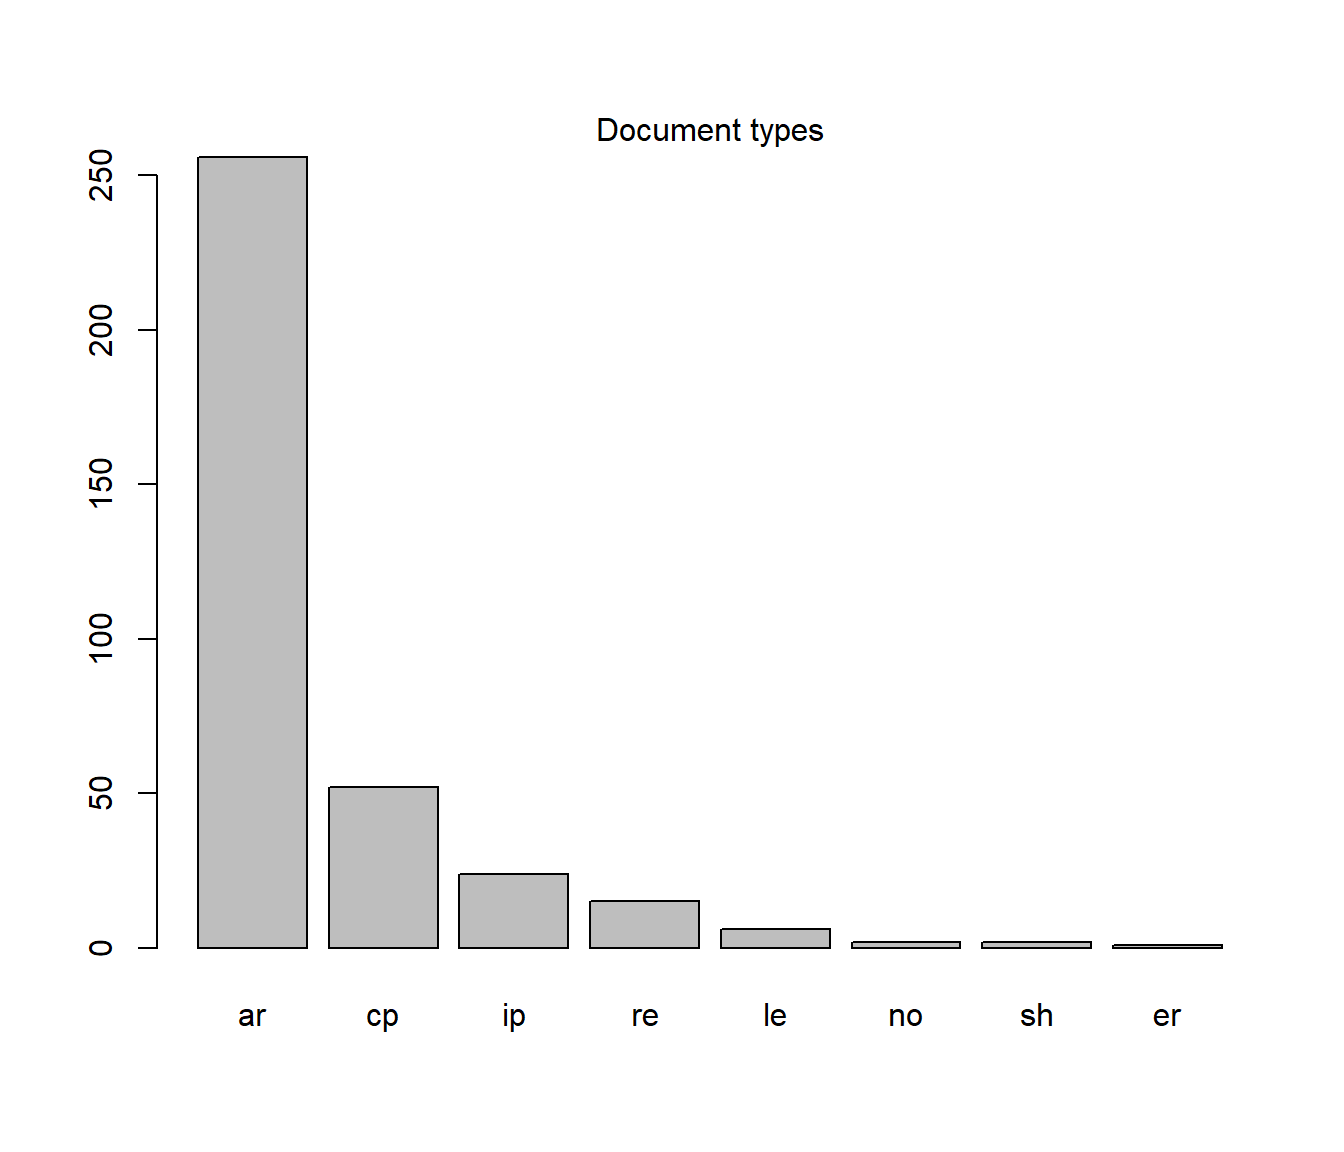
\includegraphics[width=0.7\linewidth]{22-CITAN_files/figure-latex/unnamed-chunk-13-1} \end{center}

\begin{verbatim}
## Document types:
## 
##  ar  cp  ip  re  le  no  sh  er 
## 256  52  24  15   6   2   2   1
\end{verbatim}

\begin{center}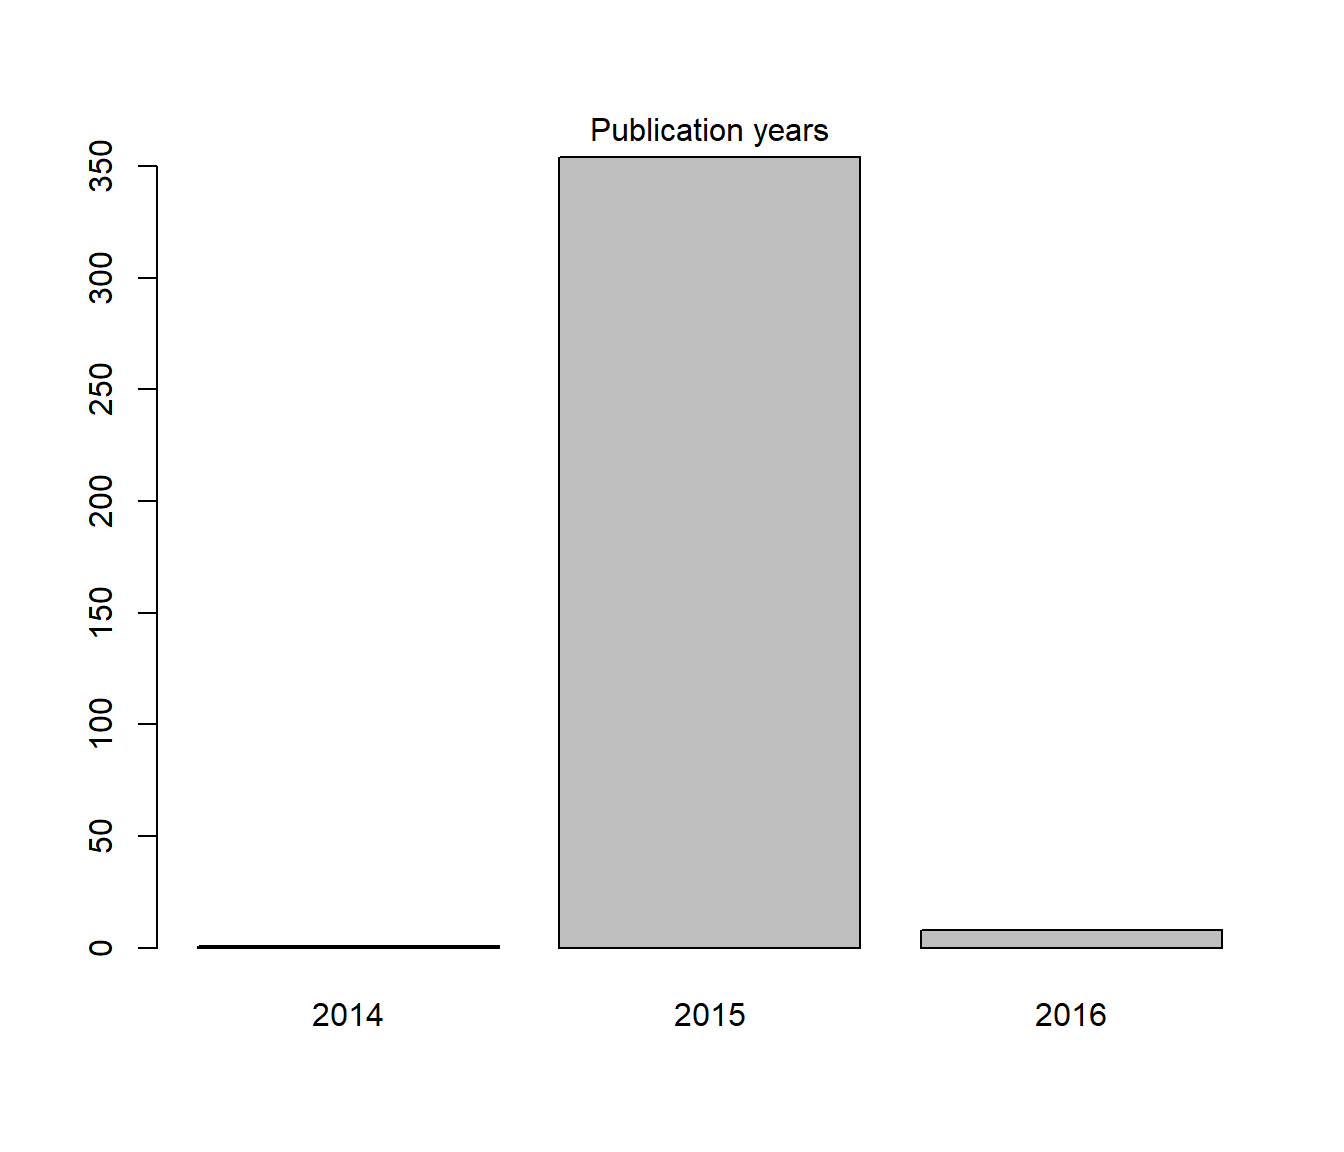
\includegraphics[width=0.7\linewidth]{22-CITAN_files/figure-latex/unnamed-chunk-13-2} \end{center}

\begin{verbatim}
## Publication years:
## 
## 2014 2015 2016 
##    1  354    8
\end{verbatim}

\begin{center}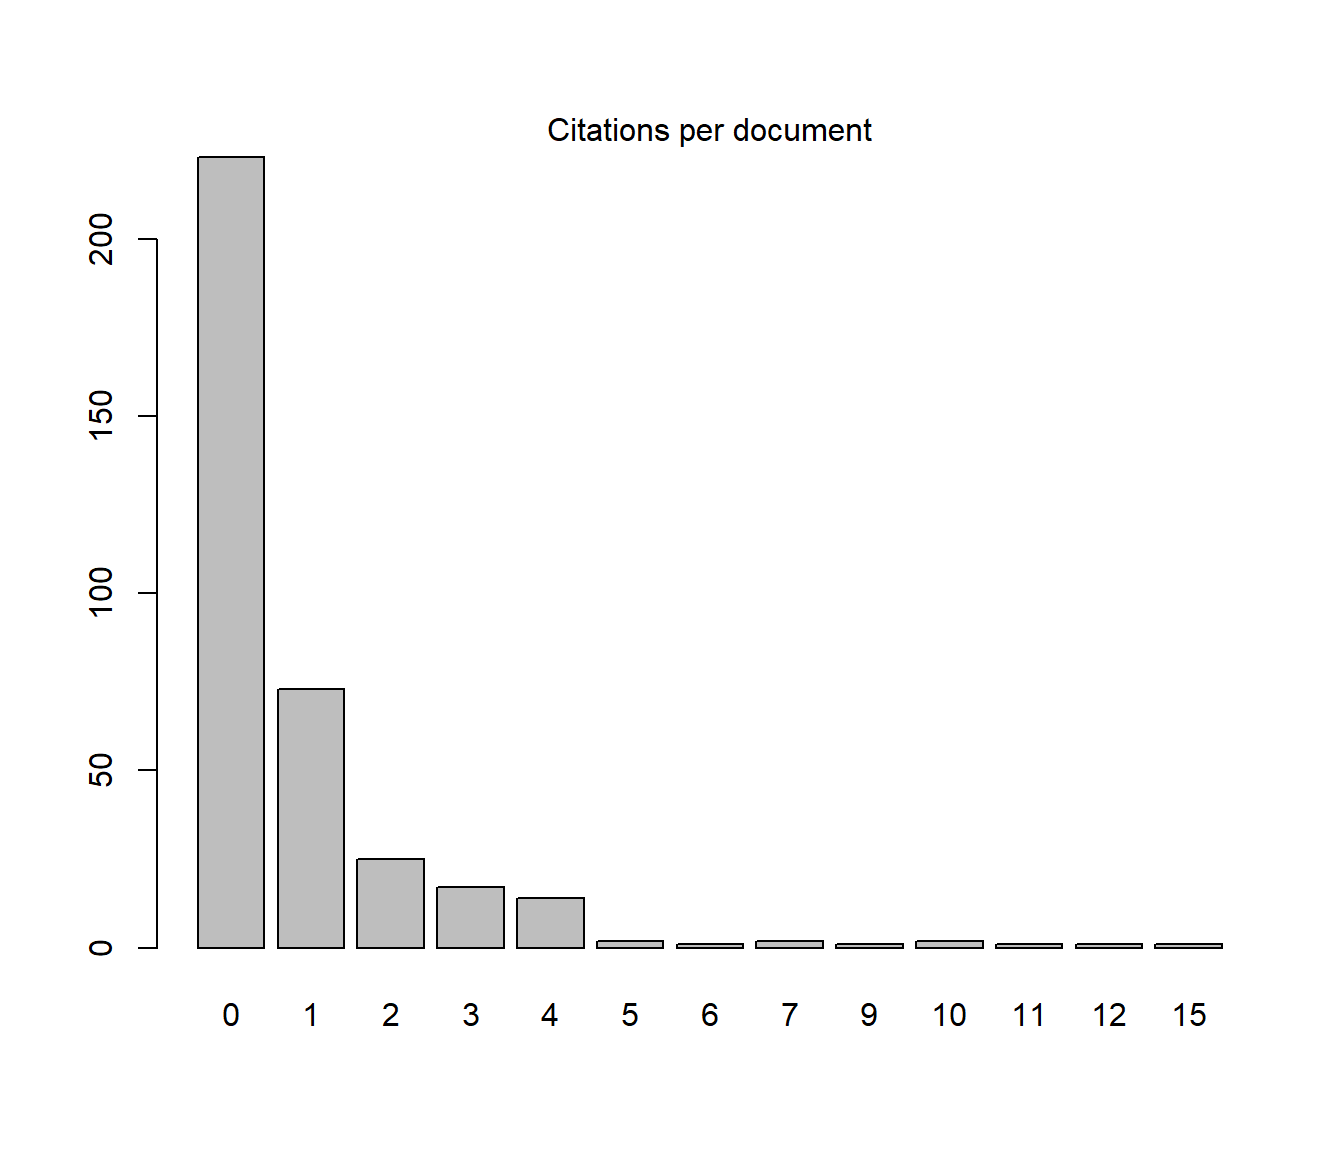
\includegraphics[width=0.7\linewidth]{22-CITAN_files/figure-latex/unnamed-chunk-13-3} \end{center}

\begin{verbatim}
## Citations per document:
## 
##   0   1   2   3   4   5   6   7   9  10  11  12  15 
## 223  73  25  17  14   2   1   2   1   2   1   1   1
\end{verbatim}

\begin{center}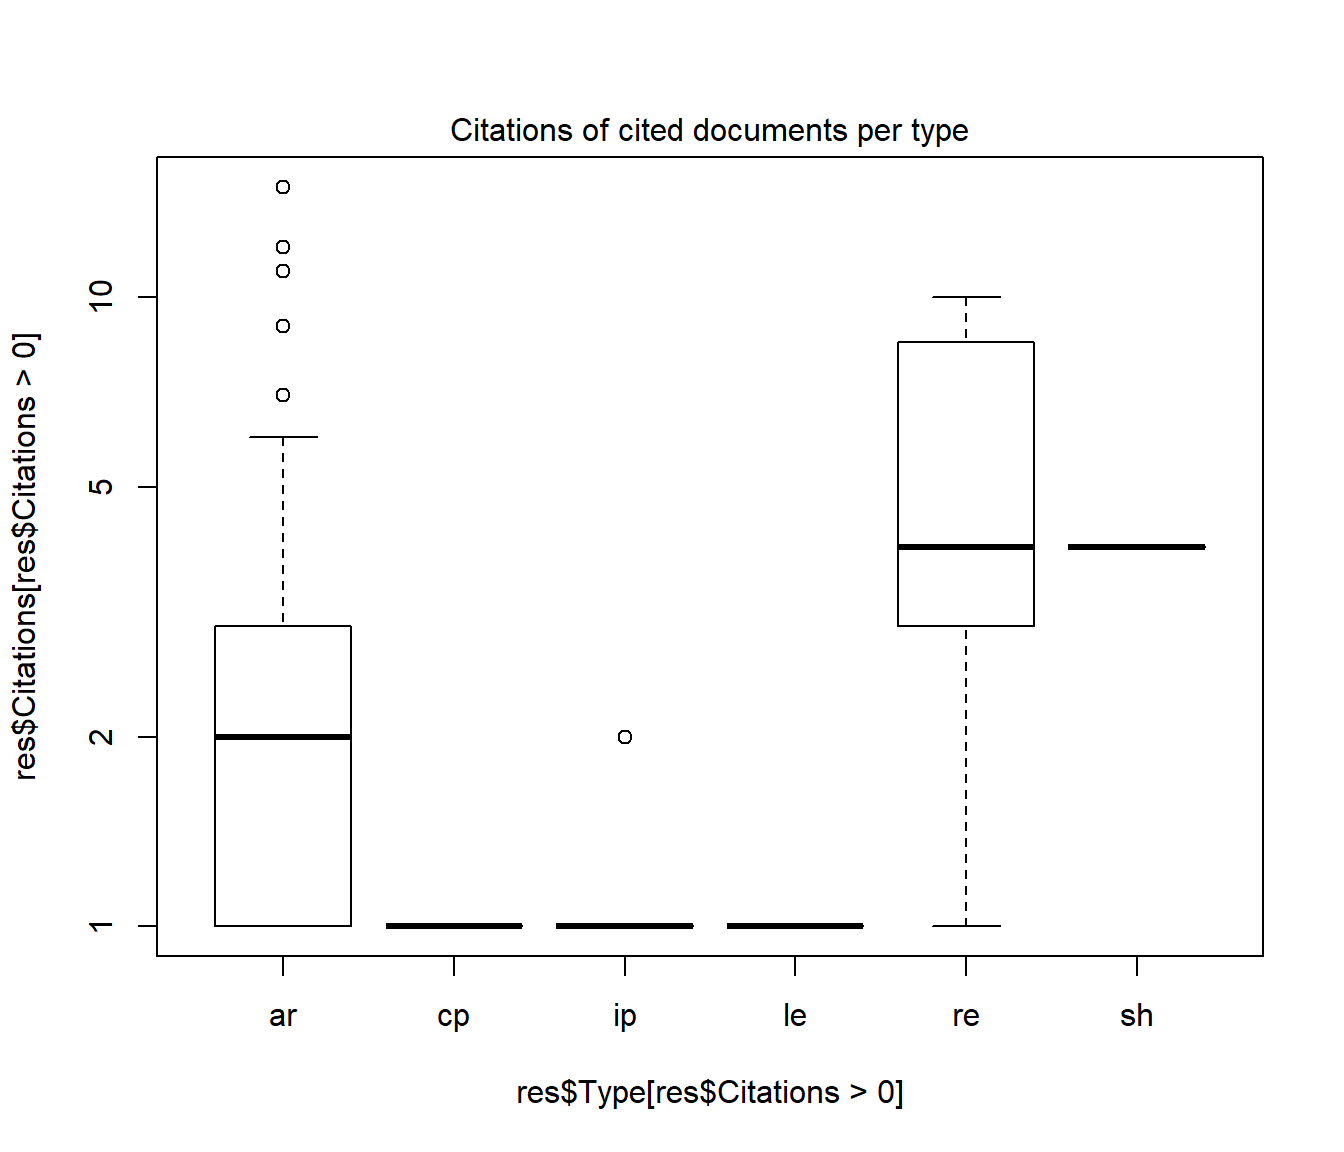
\includegraphics[width=0.7\linewidth]{22-CITAN_files/figure-latex/unnamed-chunk-13-4} \end{center}

\begin{center}\includegraphics[width=0.7\linewidth]{22-CITAN_files/figure-latex/unnamed-chunk-13-5} \end{center}

\begin{center}\includegraphics[width=0.7\linewidth]{22-CITAN_files/figure-latex/unnamed-chunk-13-6} \end{center}

\begin{verbatim}
## Categories of documents:
##          Economics, Econometrics and Finance(all) 
##                                                 8 
##                                  Engineering(all) 
##                                                45 
##                          Arts and Humanities(all) 
##                                                 9 
##                                     Medicine(all) 
##                                                43 
##                         Chemical Engineering(all) 
##                                                10 
##                             Computer Science(all) 
##                                                35 
##   Pharmacology, Toxicology and Pharmaceutics(all) 
##                                                10 
##                                             Other 
##                                                33 
##                            Materials Science(all) 
##                                                22 
##         Agricultural and Biological Sciences(all) 
##                                                27 
##                                  Mathematics(all) 
##                                                30 
## Biochemistry, Genetics and Molecular Biology(all) 
##                                                32 
##                        Environmental Science(all) 
##                                                32 
##                              Social Sciences(all) 
##                                                32 
##                        Physics and Astronomy(all) 
##                                                19 
##                                       Energy(all) 
##                                                10 
##          Business, Management and Accounting(all) 
##                                                10 
##                                   Psychology(all) 
##                                                 8 
##                                    Chemistry(all) 
##                                                51
\end{verbatim}

\begin{center}\includegraphics[width=0.7\linewidth]{22-CITAN_files/figure-latex/unnamed-chunk-13-7} \end{center}

\begin{verbatim}
## Documents per author:
## 
##    1    2    3    4    5    6    7    8    9   10   11   13   16 
## 1000  224   46   18   12    8    6    1    1    2    2    1    1
\end{verbatim}

\subsection{Otra información}\label{otra-informaciuxf3n}

Se puede obtener información acerca de los documentos producidos y las
citas recibidas correspondientes a cada autor:

\begin{Shaded}
\begin{Highlighting}[]
\NormalTok{citseq <-}\StringTok{ }\KeywordTok{lbsGetCitations}\NormalTok{(conn)}
\end{Highlighting}
\end{Shaded}

\begin{verbatim}
## Data set restrictions:
##  Survey:         <ALL>.
##  Document types: <ALL>.
## 
## Creating citation sequences... OK, 1322 of 1322 records read.
\end{verbatim}

\begin{Shaded}
\begin{Highlighting}[]
\CommentTok{# citseq <- lbsGetCitations(conn, surveyDescription="udc_2015")}
\end{Highlighting}
\end{Shaded}

Número de autores

\begin{Shaded}
\begin{Highlighting}[]
\KeywordTok{length}\NormalTok{(citseq) }
\end{Highlighting}
\end{Shaded}

\begin{verbatim}
## [1] 1322
\end{verbatim}

\begin{Shaded}
\begin{Highlighting}[]
\KeywordTok{head}\NormalTok{(}\KeywordTok{names}\NormalTok{(citseq))}
\end{Highlighting}
\end{Shaded}

\begin{verbatim}
## [1] "LÓPEZ-GARCÍA X."   "MARWAH S."         "OTERO T.P."       
## [4] "IGLESIAS M.P."     "GONZÁLEZ-RIVAS D." "BARROS CASTRO J."
\end{verbatim}

\begin{Shaded}
\begin{Highlighting}[]
\NormalTok{citseq[[}\DecValTok{4}\NormalTok{]]}
\end{Highlighting}
\end{Shaded}

\begin{verbatim}
## 229  11 
##   1   0 
## attr(,"IdAuthor")
## [1] 4
\end{verbatim}

Se pueden seleccionar autores:

\begin{Shaded}
\begin{Highlighting}[]
\NormalTok{id <-}\StringTok{ }\KeywordTok{lbsSearchAuthors}\NormalTok{(conn, }\KeywordTok{c}\NormalTok{(}\StringTok{"Cao R."}\NormalTok{, }\StringTok{"Naya S."}\NormalTok{, }\StringTok{"Naya-Fernandez S."}\NormalTok{))}
\NormalTok{id}
\end{Highlighting}
\end{Shaded}

\begin{verbatim}
## [1]   46 1193
\end{verbatim}

Obtener las citas de los trabajos de los autores seleccionados:

\begin{Shaded}
\begin{Highlighting}[]
\NormalTok{citseq2 <-}\StringTok{ }\KeywordTok{lbsGetCitations}\NormalTok{(conn, }\DataTypeTok{idAuthors=}\NormalTok{id)}
\end{Highlighting}
\end{Shaded}

\begin{verbatim}
## Data set restrictions:
##  Survey:         <ALL>.
##  Document types: <ALL>.
## 
## Creating citation sequences... OK, 2 of 2 records read.
\end{verbatim}

\begin{Shaded}
\begin{Highlighting}[]
\KeywordTok{length}\NormalTok{(citseq2)}
\end{Highlighting}
\end{Shaded}

\begin{verbatim}
## [1] 2
\end{verbatim}

Obtener los documentos relativos a los autores seleccionados:

\begin{Shaded}
\begin{Highlighting}[]
\NormalTok{id_re  <-}\StringTok{  }\KeywordTok{lbsSearchDocuments}\NormalTok{(conn, }\DataTypeTok{idAuthors=}\NormalTok{id)}
\end{Highlighting}
\end{Shaded}

Obtener información acerca de los documentos:

\begin{Shaded}
\begin{Highlighting}[]
\NormalTok{info_re <-}\StringTok{ }\KeywordTok{lbsGetInfoDocuments}\NormalTok{(conn, id_re)}
\NormalTok{info_re}
\end{Highlighting}
\end{Shaded}

\begin{verbatim}
## [[1]]
## IdDocument:    16
## AlternativeId: 2-s2.0-84947552209
## Title:         Lifetime estimation applying a kinetic model based on the generalized logistic function to biopolymers
## BibEntry:      Journal of Thermal Analysis and Calorimetry,2015,122,3,,1203,1212
## Year:          2015
## Type:          Article
## Citations:     0
## Authors:       NAYA S./46/NA, ÁLVAREZ A./518/NA, LÓPEZ-BECEIRO J./565/NA, GARCÍA-PARDO S./624/NA, TARRÍO-SAAVEDRA J./631/NA, QUINTANA-PITA S./709/NA, GARCÍA-SABÁN F.J./978/NA
## 
## [[2]]
## IdDocument:    98
## AlternativeId: 2-s2.0-84928890357
## Title:         Bootstrap testing for cross-correlation under low firing activity
## BibEntry:      Journal of Computational Neuroscience,2015,38,3,,577,587
## Year:          2015
## Type:          Article
## Citations:     1
## Authors:       ESPINOSA N./779/NA, MARIÑO J./832/NA, CUDEIRO J./1096/NA, CAO R./1193/NA, GONZÁLEZ-MONTORO A.M./1294/NA
## 
## [[3]]
## IdDocument:    127
## AlternativeId: 2-s2.0-84939982743
## Title:         Classification of wood using differential thermogravimetric analysis
## BibEntry:      Journal of Thermal Analysis and Calorimetry,2015,120,1,,541,551
## Year:          2015
## Type:          Article
## Citations:     0
## Authors:       NAYA S./46/NA, LÓPEZ-BECEIRO J./565/NA, TARRÍO-SAAVEDRA J./631/NA, FRANCISCO-FERNÁNDEZ M./766/NA, ARTIAGA R./1112/NA
\end{verbatim}

Obtener las citas de cada documento:

\begin{Shaded}
\begin{Highlighting}[]
\NormalTok{cit_re  <-}\StringTok{  }\KeywordTok{sapply}\NormalTok{(info_re,  }\ControlFlowTok{function}\NormalTok{(x)  x}\OperatorTok{$}\NormalTok{Citations)}
\NormalTok{cit_re}
\end{Highlighting}
\end{Shaded}

\begin{verbatim}
## [1] 0 1 0
\end{verbatim}

etc\ldots{}

El último paso será desconectar la BD\ldots{}

\section{Cerrar conexión}\label{cerrar-conexiuxf3n}

\begin{Shaded}
\begin{Highlighting}[]
\KeywordTok{lbsDisconnect}\NormalTok{(conn)}
\end{Highlighting}
\end{Shaded}

\chapter{Introducción al Aprendizaje
Estadístico}\label{introducciuxf3n-al-aprendizaje-estaduxedstico}

\section{Data Science}\label{data-science}

\textbf{\emph{Data Science}}: \emph{Data Mining}, \emph{Machine
Learning}, \emph{Statistical Learning}, \emph{Knowlegde Discovery},
\emph{Business Intelligence}, \ldots{}

\begin{itemize}
\item
  El conjunto de herramientas para entender y modelizar conjuntos
  (complejos) de datos.
\item
  El proceso de construir modelos a partir de los datos para aprender y
  predecir.
\item
  El proceso de descubrir patrones y obtener conocimiento a partir de
  grandes conjuntos de datos (\emph{big data}).
\item
  El arte y la ciencia del análisis inteligente de los datos.
\item
  Multidisciplicar, con importantes aportaciones estadísticas e
  informáticas.
\end{itemize}

\begin{figure}
\includegraphics[width=0.8\linewidth]{images/esquema2} \caption{Etapas del proceso}\label{fig:esquema}
\end{figure}

\subsection{Ventajas e inconvenientes}\label{ventajas-e-inconvenientes}

Ventajas:

\begin{itemize}
\item
  Flexibilidad (hay menos suposiciones sobre los datos).
\item
  Adecuado para big data.
\end{itemize}

Inconvenientes:

\begin{itemize}
\item
  Algunos métodos son poco interpretables.
\item
  Pueden aparecer problemas de sobreajuste.
\item
  Mayores problemas al extrapolar e interpolar.
\end{itemize}

La idea es ``dejar hablar a los datos'' y no ``encorsetarlos'' a priori,
dándoles mayor peso que a los modelos.

\textbf{CUIDADO}: los datos no sustituyen a la población (pueden
presentar grandes sesgos, la información disponible puede no ser
representativa de la población).

\begin{quote}
``The sheer volume of data would obviate the need of theory and even
scientific method'' --- Chris Anderson, físico y periodista, 2008
\end{quote}

\section{Métodos de aprendizaje
estadístico}\label{muxe9todos-de-aprendizaje-estaduxedstico}

\begin{itemize}
\item
  Aprendizaje no supervisado: Métodos exploratorios (sin variable
  respuesta). El objetivo principal es entender las relaciones y
  estructura de los datos.

  \begin{itemize}
  \item
    Análisis descriptivo
  \item
    Métodos de reducción de la dimensión (análisis de componentes
    principales, análisis factorial,\ldots{})
  \item
    Clúster
  \item
    Detección de datos atípicos
  \end{itemize}
\item
  Aprendizaje supervisado: Métodos predictivos (con variable respuesta).
  El objetivo principal es la construcción de modelos, principalmente
  para predecir. Dependiendo del tipo de variable respuesta:

  \begin{itemize}
  \item
    Clasificación: cualitativa
  \item
    Regresión: numérica
  \end{itemize}
\end{itemize}

\subsection{Métodos (de aprendizaje
supervisado):}\label{muxe9todos-de-aprendizaje-supervisado}

Métodos de Clasificación:

\begin{itemize}
\item
  Análisis discriminante (lineal, cuadrático), Regresión logística,
  multinomial, \ldots{}
\item
  Árboles de decisión, \emph{bagging}, \emph{random forest},
  \emph{boosting}
\item
  \emph{Support vector machines} (SVM)
\end{itemize}

Métodos de regresión:

\begin{itemize}
\item
  Modelos lineales:

  \begin{itemize}
  \item
    Regresión lineal: \texttt{lm()}, \texttt{lme()}, \texttt{biglm},
    \ldots{}
  \item
    Regresión lineal robusta: \texttt{MASS::rlm()}, \ldots{}
  \item
    Métodos de regularización (Ridge regression, Lasso):
    \texttt{glmnet}, \ldots{}
  \end{itemize}
\item
  Modelos lineales generalizados: \texttt{glm()}, \texttt{bigglm}, ..
\item
  Modelos paramétricos no lineales: \texttt{nls()}, \texttt{nlme},
  \ldots{}
\item
  Regresión local (métodos de suavizado): \texttt{loess()},
  \texttt{KernSmooth}, \texttt{sm}, \texttt{np}, \ldots{}
\item
  Modelos aditivos generalizados (GAM): \texttt{mgcv}, \texttt{gam},
  \ldots{}
\item
  Arboles de decisión, Random Forest, Boosting: \texttt{rpart},
  \texttt{randomForest}, \texttt{xgboost}, \ldots{}
\item
  Redes neuronales: \texttt{nnet}, \ldots{}
\end{itemize}

Paquetes con entornos gráficos (datos en memoria):

\begin{itemize}
\item
  R-Commander + FactoMineR: \texttt{Rcmdr},
  \texttt{RcmdrPlugin.FactoMineR}
\item
  Rattle: \texttt{rattle}
\end{itemize}

\subsection{Construcción y evaluación de los
modelos}\label{construcciuxf3n-y-evaluaciuxf3n-de-los-modelos}

El procedimiento habitual es particionar la base de datos en 2 (o
incluso en 3) conjuntos:

\begin{itemize}
\item
  Conjunto de datos de aprendizaje para construir los modelos
\item
  Conjunto de datos de (test) validación para (afinar) evaluar el
  rendimiento de los modelos
\end{itemize}

Alternativas: validación cruzada, bagging (bootstrap de las
observaciones)

En el caso de grandes conjuntos de datos las aproximaciones más
empleadas son:

\begin{itemize}
\item
  Submuestreo: la idea es que a partir de un cierto número de
  observaciones el incremento en la precisión es relativamente
  pequeño\footnote{El error de estimación suele ser de orden
    \(n^{-1/2}\) o superior, incrementar cuatro veces el número de datos
    disminuye el error de\\
    estimación a la mitad o menos}.
\item
  Computación paralela/distribuida:

  \begin{itemize}
  \item
    Resumir (paralela/distribuida) -\textgreater{} Combinar
    -\textgreater{} Modelar
  \item
    Modelar (paralela/distribuida) -\textgreater{} Combinar
  \item
    Se puede implementar mediante un sistema \emph{MapReduce} (Hadoop):
    los datos se procesan de forma distribuida mediante \emph{Mappers} y
    los resultados se combinan mediante \emph{Reducers}.
  \end{itemize}
\end{itemize}

\subsection{Matriz de confusión}\label{matriz-de-confusiuxf3n}

Para estudiar la eficiencia de un método de clasificación supervisada se
evalúa el modelo en el conjunto de datos de validación y se genera una
tabla de contingencia con las predicciones (columnas) frente a los
valores reales (filas).

\begin{longtable}[]{@{}ccc@{}}
\toprule
Observado\textbackslash{}Predicción & Positivo & Negativo\tabularnewline
\midrule
\endhead
Verdadero & Verdadero positivo & Falso negativo\tabularnewline
Falso & Falso positivo & Verdadero negativo\tabularnewline
\bottomrule
\end{longtable}

A partir de esta tabla se pueden estimar las tasas de falsos y
verdaderos negativos y positivos (caso de dos categorías).

\subsection{Predicciones frente a
observado}\label{predicciones-frente-a-observado}

Para estudiar la eficiencia de un método de regresión se evalúa el
modelo en el conjunto de datos de validación y se comparan las
predicciones frente a los valores reales

\includegraphics[width=6.38in]{images/predobs}

\begin{itemize}
\item
  Las predicciones deberían estar próximas a los valores reales \(y=x\),
  en azul.
\item
  El pseudo R-cuadrado (el cuadrado de la correlación entre las
  predicciones y los valores observados, que se corresponde con la línea
  discontinua) debería ser próximo a 1.
\end{itemize}

\section{Arboles de decisión}\label{arboles-de-decisiuxf3n}

Métodos simples y fácilmente interpretables.

\begin{itemize}
\item
  Técnica clásica de apendizaje automático (computación).
\item
  Válidos también para regresión.
\end{itemize}

Se segmentan los valores de las variables explicativas de forma
recursiva.

\begin{itemize}
\item
  Se consideran particiones binarias.
\item
  El conjunto de reglas de partición se puede resumir en un árbol.

  \includegraphics[width=4in]{images/arbol1}
\end{itemize}

La predicción será el valor más frecuente (la media en regresión) en el
nodo terminal.

\includegraphics[width=4.44in]{images/arbol2}
\includegraphics[width=4.22in]{images/arbol3}

Construcción del arbol:

\begin{itemize}
\item
  De forma recursiva se realizan particiones binarias.

  \begin{itemize}
  \item
    En cada partición se trata de mejorar la información sobre la
    respuesta.

    \begin{itemize}
    \tightlist
    \item
      El indice de Gini es una medida de la varianza total en los grupos
      (mide si hay mucha o poca igualdad dentro de los grupos).
    \end{itemize}
  \item
    Se crece el arbol hasta que cada nodo terminal tiene menos de un
    número mínimo de observaciones.
  \end{itemize}
\item
  Se poda el árbol considerando una funcion de costo basada en la
  complejidad.

  \begin{itemize}
  \item
    Evita problemas de sobreajuste, selección de variables
    explicativas\ldots{}
  \item
    Se suele emplear \textbf{validación cruzada}.
  \end{itemize}
\end{itemize}

\section{Bagging y Boosting}\label{bagging-y-boosting}

Bagging y Boosting son procedimientos generales para la reducción de la
varianza de un método estadístico de aprendizaje.

\begin{itemize}
\item
  Se trata de combinar métodos de clasificación sencillos para obtener
  un método de clasificación muy potente (y robusto).
\item
  Muy empleados con árboles de decisión.

  \begin{itemize}
  \tightlist
  \item
    Se crecen muchos árboles que luego se combinan para producir
    predicciones por consenso.
  \end{itemize}
\end{itemize}

\subsection{Bagging o agregación
Bootstrap}\label{bagging-o-agregaciuxf3n-bootstrap}

\begin{itemize}
\item
  Se remuestrea repetidamente el conjunto de datos de entrenamiento.

  \begin{itemize}
  \tightlist
  \item
    Con cada conjunto de datos (bag) se entrena un modelo.
  \end{itemize}
\item
  Las predicciones se obtienen promediando las predicciones de los
  modelos (la decisión mayoritaria en el caso de clasificación).
\item
  Se puede estimar la precisión de las predicciones con el error OOB
  (out-of-bag).
\end{itemize}

\subsection{Bosques Aleatorios}\label{bosques-aleatorios}

Los Bosques Aleatorios son una ligera modificación del bagging para el
caso de árboles de decisión.

\begin{itemize}
\item
  Además de en las observaciones se induce aleatoriedad en las
  variables.
\item
  Para evitar dependencias, los posibles predictores se seleccionan al
  azar en cada partición (e.g. \(m=\sqrt{p}\)).
\item
  No es necesario podar los árboles.
\end{itemize}

Estos métodos dificultan la interpretación.

\begin{itemize}
\item
  Se puede medir la importancia de las variables (índices de
  importancia).

  \begin{itemize}
  \tightlist
  \item
    Por ejemplo, para cada árbol se suman las reducciones en el índice
    de Gini correspondientes a las divisiones de un predictor y
    posteriormente se promedian los valores de todos los árboles.
  \end{itemize}
\end{itemize}

\subsection{Boosting}\label{boosting}

\begin{itemize}
\item
  La idea es hacer un ``aprendizaje lento''.
\item
  Los arboles se crecen de forma secuencial, se trata de mejorar la
  clasificación anterior.

  \begin{itemize}
  \tightlist
  \item
    Se utilizan arboles pequeños (en general clasificadores débiles).
  \end{itemize}
\item
  Se puede pensar que se ponderan las observaciones iterativamente, se
  asigna más peso a las que resultaron más difíciles de clasificar.
\item
  El modelo final es un modelo aditivo (media ponderada de los árboles).
\end{itemize}

\section{Support vector machines
(SVM)}\label{support-vector-machines-svm}

Este método es una generalización del denominado \textbf{clasificador de
máximo margen}.

\begin{itemize}
\item
  Si las clases se pueden separar linealmente, se escoge el hiperplano
  con el mayor margen entre las clases.

  \includegraphics[width=4.17in]{images/svm1}
\end{itemize}

Los puntos que determinan el margen (y el hiperplano) se denominan
vectores de soporte.

En el caso de que las categorías no sean linealmente separables, se
busca un clasificador de ``margen débil'', denominado
\textbf{clasificador de soporte vectorial}.

\begin{itemize}
\item
  Más robusto frente a observaciones individuales.
\item
  Mejor clasificación de la mayoría de las observaciones de
  entrenamiento.
\end{itemize}

Se incluye un parámetro adicional \(C\) que permite la mala
clasificación de algunas observaciones.

\begin{longtable}[]{@{}cr@{}}
\toprule
\includegraphics{images/svm2.png} &
\includegraphics{images/svm3.png}\tabularnewline
\(C\) grande & \(C\) pequeño\tabularnewline
\bottomrule
\end{longtable}

En ciertos casos una frontera lineal no es adecuada.

\begin{itemize}
\item
  Se transforman las variables explicativas de forma que se puedan
  separar las clases: \textbf{maquinas de soporte vectorial (SVM).}
\item
  Se consideran núcleos polinómicos, radiales, \ldots{}

  \includegraphics[width=6.72in]{images/svm4}
\end{itemize}

\section{Modelos lineales
(generalizados)}\label{modelos-lineales-generalizados}

Los modelos lineales suponen que la función de regresión es lineal:

\[Y=\beta_{0}+\beta_{1}X_{1}+\beta_{2}X_{2}+\cdots+\beta_{p}X_{p}+\varepsilon\]

El efecto de las variables explicativas sobre la respuesta es simple
(proporcional a su valor), por lo que son muy fáciles de interpretar.

Los modelos lineales generalizados son una extensión de los modelos
lineales para el caso de que la distribución condicional de la variable
respuesta no sea normal (por ejemplo discreta: Bernouilli, Binomial,
Poisson, \ldots{}).

En los modelo lineales se supone que:
\[E( Y | \mathbf{X} ) = \beta_{0}+\beta_{1}X_{1}+\beta_{2}X_{2}+\cdots+\beta_{p}X_{p}\]
En los modelos lineales generalizados se introduce una función
invertible \emph{g}, denominada función enlace (o link):
\[g\left(E(Y | \mathbf{X} )\right) = \beta_{0}+\beta_{1}X_{1}+\beta_{2}X_{2}+\cdots+\beta_{p}X_{p}\]

Cuando se dispone de un conjunto grande de posibles variables
explicativas suele ser especialmente importante determinar cuales de
estas deberían ser incluidas en el modelo de regresión. Si alguna de las
variables no contiene información relevante sobre la respuesta no se
debería incluir (se simplificaría la interpretación del modelo,
aumentaría la precisión de la estimación y se evitarían problemas como
la multicolinealidad). Se trataría entonces de conseguir un buen ajuste
con el menor número de variables explicativas posible.

Para obtener el modelo ``óptimo'' lo ideal sería evaluar todos los
modelos posibles. Si el número de variables explicativas es grande, en
lugar de emplear una búsqueda exhaustiva se puede emplear un criterio
por pasos:

\begin{itemize}
\item
  \textbf{Selección progresiva} (forward): Se parte de una situación en
  la que no hay ninguna variable y en cada paso se incluye una aplicando
  un \textbf{criterio de entrada} (hasta que ninguna de las restantes lo
  verifican).
\item
  \textbf{Eliminación progresiva} (backward): Se parte del modelo con
  todas las variables y en cada paso se elimina una aplicando un
  \textbf{criterio de salida} (hasta que ninguna de las incluidas lo
  verifican).
\item
  \textbf{Regresión paso a paso} (stepwise): El más utilizado, se
  combina un criterio de entrada y uno de salida. Normalmente se parte
  sin ninguna variable y \textbf{en cada paso puede haber una inclusión
  y una exclusión} (forward/backward).
\end{itemize}

Cuando el número de variables explicativas es muy grande (o si el tamaño
de la muestra es pequeño en comparación) pueden aparecer problemas al
emplear los métodos anteriores (incluso pueden no ser aplicables). Una
alternativa son los métodos de regularización (Ridge regression, Lasso).

\section{Métodos de
regularización}\label{muxe9todos-de-regularizaciuxf3n}

Estos métodos emplean también un modelo lineal generalizado, pero
imponen restricciones adicionales a los parámetros que los ``retraen''
(shrink) hacia cero:

\begin{itemize}
\item
  Produce una reducción en la varianza de predicción (a costa del
  sesgo).
\item
  En principio se consideran todas las variables explicativas.
\end{itemize}

Por ejemplo, en el caso del modelo lineal:
\[Y=\beta_{0}+\beta_{1}X_{1}+\beta_{2}X_{2}+\cdots+\beta_{p}X_{p}+\varepsilon\]

En lugar de ajustarlo por mínimos cuadrados (estándar), minimizando:
\[ RSS = \sum\limits_{i=1}^{n}\left(  y_{i} - \beta_0 - \beta_1 x_{1i} - \cdots - \beta_p x_{pi} \right)^{2}\]

\textbf{Ridge regression}

\begin{itemize}
\tightlist
\item
  Penalización cuadrática: \(RSS+\lambda\sum_{j=1}^{p}\beta_{j}^{2}\).
\end{itemize}

\textbf{Lasso}

\begin{itemize}
\item
  Penalización en valor absoluto:
  \(RSS+\lambda\sum_{j=1}^{p}|\beta_{j}|\).
\item
  Normalmente asigna peso nulo a algunas variables (selección de
  variables).
\end{itemize}

El parámetro de penalización se selecciona por \textbf{validación
cruzada}.

\begin{itemize}
\tightlist
\item
  Normalmente estandarizan las variables explicativas (coeficientes en
  la misma escala).
\end{itemize}

Consideraremos como ejemplo el conjunto de datos \emph{hatco.RData} que
contiene observaciones de clientes de la compañía de distribución
industrial (Compañía Hair, Anderson y Tatham).

\begin{Shaded}
\begin{Highlighting}[]
\KeywordTok{load}\NormalTok{(}\StringTok{'data/hatco.RData'}\NormalTok{)}
\KeywordTok{as.data.frame}\NormalTok{(}\KeywordTok{attr}\NormalTok{(hatco, }\StringTok{"variable.labels"}\NormalTok{))}
\end{Highlighting}
\end{Shaded}

\begin{verbatim}
##          attr(hatco, "variable.labels")
## empresa                         Empresa
## tamano             Tamaño de la empresa
## adquisic      Estructura de adquisición
## tindustr              Tipo de industria
## tsitcomp    Tipo de situación de compra
## velocida           Velocidad de entrega
## precio                 Nivel de precios
## flexprec        Flexibilidad de precios
## imgfabri          Imagen del fabricante
## servconj              Servicio conjunto
## imgfvent     Imagen de fuerza de ventas
## calidadp            Calidad de producto
## fidelida   Porcentaje de compra a HATCO
## satisfac            Satisfacción global
## nfidelid        Nivel de compra a HATCO
## nsatisfa          Nivel de satisfacción
\end{verbatim}

Consideraremos como respuesta la variable \emph{fidelida} y como
variables explicativas el resto de variables continuas menos
\emph{satisfac}.

\begin{Shaded}
\begin{Highlighting}[]
\KeywordTok{library}\NormalTok{(glmnet)}
\end{Highlighting}
\end{Shaded}

El paquete \texttt{glmnet} no emplea formulación de modelos, hay que
establecer la respuesta \texttt{y} y las variables explicativas
\texttt{x} (se puede emplear la función \texttt{model.matrix()} para
construir \texttt{x}, la matriz de diseño, a partir de una fórmula). En
este caso, eliminamos también la última fila por tener datos faltantes:

\begin{Shaded}
\begin{Highlighting}[]
\NormalTok{x <-}\StringTok{ }\KeywordTok{as.matrix}\NormalTok{(hatco[}\OperatorTok{-}\DecValTok{100}\NormalTok{, }\DecValTok{6}\OperatorTok{:}\DecValTok{12}\NormalTok{])}
\NormalTok{y <-}\StringTok{ }\NormalTok{hatco}\OperatorTok{$}\NormalTok{fidelida[}\OperatorTok{-}\DecValTok{100}\NormalTok{]}
\end{Highlighting}
\end{Shaded}

\subsection{Ridge Regression}\label{ridge-regression}

Ajustamos un modelo de regresión ridge con la función \texttt{glmnet}
con \texttt{alpha=0} (ridge penalty).

\begin{Shaded}
\begin{Highlighting}[]
\NormalTok{fit.ridge <-}\StringTok{ }\KeywordTok{glmnet}\NormalTok{(x, y, }\DataTypeTok{alpha =} \DecValTok{0}\NormalTok{)}
\KeywordTok{plot}\NormalTok{(fit.ridge, }\DataTypeTok{xvar =} \StringTok{"lambda"}\NormalTok{, }\DataTypeTok{label =} \OtherTok{TRUE}\NormalTok{)}
\end{Highlighting}
\end{Shaded}

\includegraphics{23-StatisticalLearning_files/figure-latex/unnamed-chunk-9-1.pdf}

Para seleccionar el parámetro de penalización por validación cruzada se
puede emplear la función \texttt{cv.glmnet}.

\begin{Shaded}
\begin{Highlighting}[]
\NormalTok{cv.ridge <-}\StringTok{ }\KeywordTok{cv.glmnet}\NormalTok{(x, y, }\DataTypeTok{alpha =} \DecValTok{0}\NormalTok{)}
\KeywordTok{plot}\NormalTok{(cv.ridge)}
\end{Highlighting}
\end{Shaded}

\includegraphics{23-StatisticalLearning_files/figure-latex/unnamed-chunk-10-1.pdf}

En este caso el parámetro sería:

\begin{Shaded}
\begin{Highlighting}[]
\NormalTok{cv.ridge}\OperatorTok{$}\NormalTok{lambda.1se}
\end{Highlighting}
\end{Shaded}

\begin{verbatim}
## [1] 2.749868
\end{verbatim}

y el modelo resultante contiene todas las variables explicativas:

\begin{Shaded}
\begin{Highlighting}[]
\KeywordTok{coef}\NormalTok{(cv.ridge)}
\end{Highlighting}
\end{Shaded}

\begin{verbatim}
## 8 x 1 sparse Matrix of class "dgCMatrix"
##                     1
## (Intercept) 2.4799000
## velocida    1.6053747
## precio      0.7733925
## flexprec    2.4462308
## imgfabri    0.2837000
## servconj    3.9801496
## imgfvent    1.1232130
## calidadp    0.1245096
\end{verbatim}

\subsection{Lasso}\label{lasso}

Ajustamos un modelo lasso también con la función \texttt{glmnet} (con la
opción por defecto \texttt{alpha=1}, lasso penalty).

\begin{Shaded}
\begin{Highlighting}[]
\NormalTok{fit.lasso <-}\StringTok{ }\KeywordTok{glmnet}\NormalTok{(x,y)}
\KeywordTok{plot}\NormalTok{(fit.lasso, }\DataTypeTok{xvar =} \StringTok{"lambda"}\NormalTok{, }\DataTypeTok{label =} \OtherTok{TRUE}\NormalTok{)}
\end{Highlighting}
\end{Shaded}

\includegraphics{23-StatisticalLearning_files/figure-latex/unnamed-chunk-13-1.pdf}

Seleccionamos el parámetro de penalización por validación cruzada.

\begin{Shaded}
\begin{Highlighting}[]
\NormalTok{cv.lasso <-}\StringTok{ }\KeywordTok{cv.glmnet}\NormalTok{(x,y)}
\KeywordTok{plot}\NormalTok{(cv.lasso)}
\end{Highlighting}
\end{Shaded}

\includegraphics{23-StatisticalLearning_files/figure-latex/unnamed-chunk-14-1.pdf}

En este caso el modelo resultante solo contiene 4 variables
explicativas:

\begin{Shaded}
\begin{Highlighting}[]
\KeywordTok{coef}\NormalTok{(cv.lasso)}
\end{Highlighting}
\end{Shaded}

\begin{verbatim}
## 8 x 1 sparse Matrix of class "dgCMatrix"
##                     1
## (Intercept) 4.4757712
## velocida    0.1020531
## precio      .        
## flexprec    2.7202485
## imgfabri    .        
## servconj    6.4044378
## imgfvent    0.4651076
## calidadp    .
\end{verbatim}

\section{Regresión no paramétrica}\label{regresiuxf3n-no-paramuxe9trica}

No se supone ninguna forma concreta en el efecto de las variables
explicativas: \[Y=f\left(  \mathbf{X}\right)  +\varepsilon,\] con
\emph{f} función ``cualquiera'' (suave).

\begin{itemize}
\item
  Métodos disponibles en \texttt{R}:

  \begin{itemize}
  \item
    Regresión local (métodos de suavizado): \texttt{loess()},
    \texttt{KernSmooth}, \texttt{sm}, \ldots{}
  \item
    Modelos aditivos generalizados (GAM): \texttt{gam}, \texttt{mgcv},
    \ldots{}
  \item
    \ldots{}
  \end{itemize}
\end{itemize}

\subsection{Modelos aditivos}\label{modelos-aditivos}

Se supone que:
\[Y=\beta_{0}+f_{1}\left(  \mathbf{X}_{1}\right)  +f_{2}\left(  \mathbf{X}_{2}\right)  +\cdots+f_{p}\left(  \mathbf{X}_{p}\right)  +\varepsilon\text{,}\]
con \(f_{i},\) \(i=1,...,p,\) funciones cualesquiera.

\begin{itemize}
\item
  Los modelos lineales son un caso particular considerando
  \(f_{i}(x) = \beta_{i}x\).
\item
  Son mucho más flexibles pero siguen siendo fáciles de interpretar.
\item
  Adicionalmente se puede considerar una función link: \textbf{Modelos
  aditivos generalizados} (GAM)

  \begin{itemize}
  \item
    Hastie, T.J. y Tibshirani, R.J. (1990). Generalized Additive Models.
    Chapman \& Hall.
  \item
    Wood, S. N. (2006). Generalized Additive Models: An Introduction
    with R. Chapman \& Hall/CRC
  \end{itemize}
\end{itemize}

Utilizaremos como ejemplo el conjunto de datos \texttt{Prestige} de la
librería \texttt{carData} (Companion to Applied Regression Data Sets,
paquete \texttt{car}). Se tratará de explicar \texttt{prestige}
(puntuación de ocupaciones obtenidas a traves de una encuesta) a partir
de \texttt{income} (media de ingresos en la ocupación) y
\texttt{education} (media de los años de educación).

\begin{Shaded}
\begin{Highlighting}[]
\KeywordTok{library}\NormalTok{(mgcv)}
\KeywordTok{data}\NormalTok{(Prestige, }\DataTypeTok{package =} \StringTok{"carData"}\NormalTok{)}
\NormalTok{modelo <-}\StringTok{ }\KeywordTok{gam}\NormalTok{(prestige }\OperatorTok{~}\StringTok{ }\KeywordTok{s}\NormalTok{(income) }\OperatorTok{+}\StringTok{ }\KeywordTok{s}\NormalTok{(education), }\DataTypeTok{data =}\NormalTok{ Prestige)}
\KeywordTok{summary}\NormalTok{(modelo)}
\end{Highlighting}
\end{Shaded}

\begin{verbatim}
## 
## Family: gaussian 
## Link function: identity 
## 
## Formula:
## prestige ~ s(income) + s(education)
## 
## Parametric coefficients:
##             Estimate Std. Error t value Pr(>|t|)    
## (Intercept)  46.8333     0.6889   67.98   <2e-16 ***
## ---
## Signif. codes:  0 '***' 0.001 '**' 0.01 '*' 0.05 '.' 0.1 ' ' 1
## 
## Approximate significance of smooth terms:
##                edf Ref.df     F  p-value    
## s(income)    3.118  3.877 14.61 1.53e-09 ***
## s(education) 3.177  3.952 38.78  < 2e-16 ***
## ---
## Signif. codes:  0 '***' 0.001 '**' 0.01 '*' 0.05 '.' 0.1 ' ' 1
## 
## R-sq.(adj) =  0.836   Deviance explained = 84.7%
## GCV = 52.143  Scale est. = 48.414    n = 102
\end{verbatim}

En este caso la función \texttt{plot} representa los efectos (parciales)
estimados de cada covariable:

\begin{Shaded}
\begin{Highlighting}[]
\NormalTok{par.old <-}\StringTok{ }\KeywordTok{par}\NormalTok{(}\DataTypeTok{mfrow =} \KeywordTok{c}\NormalTok{(}\DecValTok{1}\NormalTok{, }\DecValTok{2}\NormalTok{))}
\KeywordTok{plot}\NormalTok{(modelo, }\DataTypeTok{shade =} \OtherTok{TRUE}\NormalTok{) }\CommentTok{# }
\end{Highlighting}
\end{Shaded}

\includegraphics{23-StatisticalLearning_files/figure-latex/unnamed-chunk-17-1.pdf}

\begin{Shaded}
\begin{Highlighting}[]
\KeywordTok{par}\NormalTok{(par.old)}
\end{Highlighting}
\end{Shaded}

\section{Redes neuronales}\label{redes-neuronales}

Se trata de imitar el funcionamiento del cerebro de un ser vivo.

\begin{itemize}
\item
  Neuronas organizadas en capas que interactuan por medio de pesos.
\item
  Capa de entrada, capas ocultas y capa de salida.

  \includegraphics[width=6.88in]{images/nn}
\end{itemize}

Son modelos hiperparametrizados de difícil interpretación.

\begin{itemize}
\tightlist
\item
  Hay distintos métodos de aprendizaje (estimación de los pesos)
\end{itemize}

\section{Bibliografía}\label{bibliografuxeda}

\begin{itemize}
\item
  Efron, B. y Hastie, T. (2016).
  \href{http://web.stanford.edu/~hastie/CASI/}{Computer age statistical
  inference}. Cambridge University Press.
\item
  Hastie, T., Tibshirani, R. y Friedman, J. (2017).
  \href{https://web.stanford.edu/~hastie/ElemStatLearn}{The Elements of
  Statistical Learning: Data Mining, Inference, and Prediction}.
  Springer.
\item
  James, G., Witten, D., Hastie, T. y Tibshirani, R. (2017).
  \href{http://faculty.marshall.usc.edu/gareth-james/ISL}{An
  Introduction to Statistical Learning: with Aplications in R}.
  Springer.
\item
  Torgo, L. (2011). Data Mining with R: Learning with Case Studies.
  Chapman \& Hall/CRC Press.
\item
  Williams, G. (2011). Data Mining with Rattle and R. Springer.
\end{itemize}

\bibliography{book.bib,packages.bib}

\end{document}
